%% Based on a TeXnicCenter-Template by Tino Weinkauf.
%%%%%%%%%%%%%%%%%%%%%%%%%%%%%%%%%%%%%%%%%%%%%%%%%%%%%%%%%%%%%

%%%%%%%%%%%%%%%%%%%%%%%%%%%%%%%%%%%%%%%%%%%%%%%%%%%%%%%%%%%%%
%% HEADER
%%%%%%%%%%%%%%%%%%%%%%%%%%%%%%%%%%%%%%%%%%%%%%%%%%%%%%%%%%%%%
\documentclass[a4paper,oneside,11pt]{report}

%% Language %%%%%%%%%%%%%%%%%%%%%%%%%%%%%%%%%%%%%%%%%%%%%%%%%
\usepackage[english]{babel}
\usepackage[T1]{fontenc}
\usepackage[utf8]{inputenc}
%\usepackage[ansinew]{inputenc}
\usepackage{mathptmx} 


%% Packages for Graphics & Figures %%%%%%%%%%%%%%%%%%%%%%%%%%
\usepackage{graphicx} %%For loading graphic files
\graphicspath{{./graphics/}}
\usepackage{placeins} %Used for Float Barriers


%% Math Packages %%%%%%%%%%%%%%%%%%%%%%%%%%%%%%%%%%%%%%%%%%%%
\usepackage{amsmath}
\usepackage{amsthm}
\usepackage{amsfonts}
\usepackage{amssymb}%


%% Line Spacing %%%%%%%%%%%%%%%%%%%%%%%%%%%%%%%%%%%%%%%%%%%%%
\usepackage{setspace}
\onehalfspacing       %% 1.5-spacing
%Paragraph Spacing
\setlength{\parindent}{0mm}
\setlength{\parskip}{1em}



%% Other Packages %%%%%%%%%%%%%%%%%%%%%%%%%%%%%%%%%%%%%%%%%%%


\usepackage{geometry} %Page margins
\geometry{
left=30mm,
right=30mm,
top=60mm,
bottom=30mm
} %Title page margins
%Create Hyperlinks 
\usepackage{hyperref}
\hypersetup{
    colorlinks,
    citecolor=black,
    filecolor=black,
    linkcolor=black,
    urlcolor=black
}
\usepackage{multirow} % Multirow tables
\usepackage[toc]{appendix}

%Fancy Headers
\usepackage{fancyhdr,ragged2e}
\fancyhead{}
%\lhead{\parbox[t]{0.6\textwidth}{\RaggedRight\rightmark\strut}}
%\rhead{\parbox[t]{0.6\textwidth}{\RaggedLeft\leftmark\strut}}
%\setlength{\headheight}{5\baselineskip}
%\lhead{\parbox[t]{0.7\textwidth}{\RaggedRight\rightmark\strut}}
\rhead{\parbox[t]{0.7\textwidth}{\fontsize{9}{12} \selectfont \RaggedLeft\leftmark\strut}}
\renewcommand{\headrulewidth}{1pt}
\pagestyle{fancy} %%Fancy headings

%Renew the equation reference command and define a figure ref command
\renewcommand{\eqref}[1]{Eq. (\ref{#1})} 
\newcommand{\figref}[1]{Fig. \ref{#1}}
\newcommand{\tabref}[1]{Table \ref{#1}}

%%%%%%%%%%%%%%%%%%%%%%%%%%%%%%%%%%%%%%%%%%%%%%%%%%%%%%%%%%%%%
%% DOCUMENT
%%%%%%%%%%%%%%%%%%%%%%%%%%%%%%%%%%%%%%%%%%%%%%%%%%%%%%%%%%%%%
\begin{document}

\pagestyle{empty} %No headings for the first pages.


%% Title Page %%%%%%%%%%%%%%%%%%%%%%%%%%%%%%%%%%%%%%%%%%%%%%%
\begin{titlepage}
%% Based on a TeXnicCenter-Template by Tino Weinkauf.
%%%%%%%%%%%%%%%%%%%%%%%%%%%%%%%%%%%%%%%%%%%%%%%%%%%%%%%%%%%%%


\begin{titlepage}
\begin{center}
\pagenumbering{}

{\LARGE\textsc{Autonomous Control of Multi-rotor Unmanned Aerial Vehicles}\\}

\vspace{1cm}

\Large
\textsc{
by\\[0.5\baselineskip]
Lachlan Drake\\}

\vspace{1cm}
\textsc{3 December, 2021}\\ %%Date - better you write it yourself.

\vspace{1cm}
\textsc{Supervisor:\\
Associate Professor José De Dona}\\

\vspace{1cm}

\includegraphics[height=5cm]{UoN.png}

\vspace{2cm}
\small\textsc{A thesis submitted in partial fulfilment of the requirements for\\ the degree of Bachelor of Engineering in Electrical Engineering\\ at The University of Newcastle, Australia}

\clearpage
\end{center}

\end{titlepage}

\end{titlepage}

\newgeometry{
left=30mm,
right=30mm,
top=30mm,
bottom=30mm
} %Body margins

%%Front Matter 
%%%%%%%%%%%%%%%%%%%%%%%%%%%%%%%%%%%%%%%%%
\pagenumbering{roman}


\chapter*{Abstract}\label{Abstract}
\addcontentsline{toc}{chapter}{Abstract}
\clearpage




\chapter*{Acknowledgements}\label{Acknowledgements}
\addcontentsline{toc}{chapter}{Acknowledgements}

I would like to express my gratitude to all those who have supported me through my journey over the preceding year.

Firstly I would like to thank my supervisor Jos\'e De Dona. Despite the additional difficulty of unpredictable lockdowns, Jos\'e made every effort to be available both virtually and face-to-face (when possible) and provided invaluable guidance throughout the year. Without his insight and experience this project would not have been possible.

I would also like to extend my gratitude to all of the academic staff who have taught and guided me throughout my studies.

Lastly, I would like to thank all my family and friends for their support throughout this challenging year. I would especially like to thank my fianc\'ee for her love and support throughout the year. 


\clearpage




\chapter*{COVID Impact Statement}\label{COVIDStatement}
\addcontentsline{toc}{chapter}{COVID Impact Statement}

The Coronavirus (COVID-19) pandemic has harshly impacted the world in many ways for the last couple years. Although Australia has been extremely fortunate in avoiding the worst of the pandemic, there were a number of limitations imposed by the pandemic and related lockdowns upon this project. Due to being unable to access lab equipment for a significant period of time, this project was certainly made more difficult. The main effects imposed upon the project are summarised below:
\begin{itemize}
  \item Limited access to equipment for testing hardware, debugging, soldering and connecting sensors, etc. Resulting in larger amounts of time and effort being necessary to perform hardware-related tasks.
  \item An overall lack of space for storing and working on hardware.
  \item Inability to perform flight testing due to lockdowns. Unable to legally visit an open space which would be suitable for flight testing. Living in an apartment block with limited space meant that flight testing in any kind of unobstructed space was next to impossible during the lockdown period.
	\item Delays in component delivery and lack of availability. Due to the overstretched postal service,  there were significant delays (4-5 weeks) in delivery of sensors and components.
\end{itemize}

\clearpage




\chapter*{Contributions}\label{Contributions}
\addcontentsline{toc}{chapter}{Contributions}
My main contributions to the project are summarised below:
\begin{itemize}
\item Performed a comprehensive literature review of current multi-rotor modelling methods, control techniques and sensor fusion algorithms.
\item Derived a model for a hexacopter aircraft based upon Newton-Euler mechanics and implemented the model in Simulink.
\item Developed a PID control system for a hexacopter and implemented the system in Simulink.
\item Derived a control system based on the backstepping technique and implemented this system in Simulink.
\item Applied the extended Kalman filter to develop a GPS-reliant sensor fusion algorithm for use both in simulation and with recorded data.
\item Developed a second sensor fusion algorithm for use in situations where GPS is either unavailable or unreliable.
\item Installed hardware and configured software on a custom hexacopter vehicle with a commercial flight controller.
\item Performed test flights to record sensor data to verify the sensor fusion algorithms.
\end{itemize}

\par\noindent\makebox[2.5in]{\hrulefill} \hfill\makebox[2.0in]{\hrulefill}%
    \par\noindent\makebox[2.5in][l]{Lachlan Drake}      \hfill\makebox[2.0in][l]{Jos\'e De Dona}%
\clearpage





%% Table of Contents %%%%%%%%%%%%%%%%%%%%%%%%%%%%%%%%%%%%%%%
\setlength{\parskip}{0mm} %Distance between listed sections
\tableofcontents %Table of contents
\cleardoublepage %The first chapter should start on an odd page.



%% Document Body %%%%%%%%%%%%%%%%%%%%%%%%%%%%%%%%%%%%%%%%%%%%%%%%%
\setlength{\parskip}{1em} %Reinstate paragraph spacing
\pagestyle{fancy} %Now display headings
\pagenumbering{arabic} %Body page numbers
\setlength{\parskip}{1em}


\chapter{Introduction}
\textit{This chapter discusses the motivation for this project and potential applications of the results. An outline of this thesis is also presented.}\\

\section{Project Motivation}
Unmanned Aerial Vehicles (UAVs) allow tasks to be undertaken in difficult to access areas or risky environments without endangering human life. In many current applications, a human operator is required for remote control of the vehicle. However, with current technological advances in automation, it is becoming viable to use UAVs which operate completely autonomously i.e. without a human operator. This has the potential to improve the safety, efficiency, reliability, and cost of many processes. However, autonomous control of an aerial vehicle is a complex problem requiring the consideration of many areas of research, including but not limited to: modelling, control law design, sensor fusion, navigation, collision avoidance and fault tolerance.\\

UAVs were originally developed and used mainly by military organisations, beginning with the Sperry Aerial Torpedo developed during World War I for the US Navy, a radio-controlled biplane designed to be used as a flying bomb \cite{Stoff2001}. This was followed by decades of development leading to vehicles used for aerial target practice, reconnaissance, and remote bombing. However, in recent decades there has been an increased interest in the use of UAVs for both commercial and scientific applications. Commercial applications include surveying, aerial photography/videography, package delivery and pesticide spraying. UAVs are increasingly being utilised in many industries from mining to agriculture. Technological advances in computing and electronics have decreased the cost of UAVs and this has resulted in a large selection of vehicles being more widely available to hobbyists, not just large companies. Scientific research has also benefited from the use of UAVs, with applications including monitoring bodies of water for algal blooms, identifying plant species, monitoring coastal erosion and tracking/counting animal populations. One recent study \cite{Raoult2018} uses UAVs to track aquatic vertebrates without using invasive tagging methods. Even more recently, the first unmanned flights on another planet were completed by NASA’s Ingenuity helicopter on Mars \cite{Johnson2021}, demonstrating that UAV technology could be a viable option for extra-terrestrial exploration in the near future. Similarly, NASA has a mission planned for launch in 2026 to send a multi-rotor aircraft, named Dragonfly, to explore Titan – the largest moon of Saturn\cite{Hautaluoma2019}.  The versatility of UAVs results in an almost limitless number of applications for their use.\\

UAV operation allows tasks to be undertaken in difficult to access areas or risky environments without endangering human life. In many current applications, a human operator is required for control of the vehicle. However, with current technological advances in automation, it is becoming viable to use UAVs which operate completely autonomously i.e. without a human operator. This has the potential to improve the safety, efficiency, reliability and cost of many processes.\\

UAVs come in many different configurations with the main classifications being fixed-wing and rotor, however there also exist some hybrid configurations. Rotorcraft have the advantage of being able to perform Vertical Take-Off and Landing (VTOL), i.e. they do not require a runway for take off and landing. Also, rotorcraft are able to hover in a fixed position, as opposed to fixed wing vehicles which need to continually move to generate lift. On the other hand, fixed-wing vehicles are generally able to travel at much higher speeds and can fly at higher altitudes. \\

Further, within each of these classifications there exist many different configurations. The defining characteristic of rotorcraft configurations is the number of rotors present on the vehicle. There is an almost limitless number of configurations from single rotor vehicles up to octocopters (8 rotors) and beyond. The topic of this thesis is centred around unmanned multi-rotor vehicles and will begin with an overview of the basic dynamics of these systems. These ideas will then be extended to the specific configuration of a six-rotor vehicle - the hexacopter.

\section{Thesis Outline}
This thesis is divided into seven chapters. The contents of the chapters (including this one) are summarised below:
\begin{itemize}
\item Chapter One introduces the main concepts surrounding unmanned aerial vehicles and outlines the motivation for the project.
\item Chapter Two investigates the technical background necessary for the concepts covered in this thesis. The key theory is summarised and useful formulae are presented and explained. The current literature around modelling, control and state estimation for multi-rotor vehicles is also evaluated.
\item Chapter Three develops a comprehensive mathematical model to describe the dynamics of a general multi-rotor vehicle. This is then extended to a specific configuration  with six propellers known as a hexacopter.
\item Chapter Four explores the control of the hexacopter through the development and testing of a number of progressively more complex control systems. The chapter begins with the development of a PID controller. Next, backstepping control theory is used to stabilise the system. Then integral action is added to the backstepping controller and finally the issue presented by actuator saturation is addressed.
\item Chapter Five addresses the estimation of the systems states using extended Kalman filtering techniques. First, an algorithm which relies upon GPS data is developed. Next, an alternative algorithm which uses an optical flow sensor is developed and tested for use in situations where GPS signal is not available.
\item Chapter Six discusses a custom hexacopter hardware platform. This hexacopter is then used for gathering flight data for processing with the state estimator algorithms.
\item Chapter Seven, the final chapter, summarises the results of the project and discusses future extensions.
\end{itemize}

\clearpage




\chapter{Background}
\textit{This chapter serves two main purposes. Firstly, it evaluates the available literature surrounding the effectiveness of techniques for modelling, control and state estimation in unmanned aerial vehicles and related platforms. Secondly, it introduces the key mathematical, physical and technical concepts necessary for the discussion in the following chapters.}

\section{Modelling Multi-Rotor Vehicles}
\subsection{Modelling Approaches}
In order to control a system, it is first necessary to have an understanding of the dynamics of the system. There are multiple methods used for developing mathematical models in order to describe the dynamics of multi-rotor vehicles. The Newtonian approach uses forces and torques in order to describe the system, whereas the Lagrangian approach utilises energies \cite{Raine2017}.\\

 Further, attitude of the vehicle can be described by using either Euler angles or quaternions. Euler angles express attitude with three angles, each representing the rotation in 3D space around each axis. Alternatively, quaternion algebra is used to represent attitude with four scalar variables representing a point on the unit sphere \cite{Voight2021}. Euler representation is more intuitive, however quaternion representation has the advantage of avoiding a problem known as gimbal lock which arises when two of the Euler rotation axes align, resulting in a loss of a degree of freedom.\\

Newton-Euler formalism combines Newtonian mechanics and Euler angle representation in order to describe the rotational and translational dynamics of rigid bodies. This approach is commonly used to develop a mathematical model for multi-rotor vehicles. The main advantage of this method is that it is simple to understand. Alternatively, using Euler-Lagrange formalism results in a more compact derivation \cite{Zhang2014}. \\

Multiple studies demonstrate the effectiveness of multi-rotor models developed using Newton-Euler formalism \cite{Bouabdallah2006}, \cite{Baranek2012}. Therefore, this thesis will utilise this method. Due to the uncomplicated nature of this formulation, identifying issues in the model and debugging simulations will, in general, be easier as compared to similar models formed using quaternion algebra or Lagrangian techniques.



\subsection{Newton-Euler Equations}
The Basic Kinematic Equation (BKE) is used in Newton-Euler dynamics to describe the relative motion of two reference frames \cite{Ardema2006}. The BKE is given in Equation \ref{eqn:BKE1}:
\begin{equation}\label{eqn:BKE1} 
\frac{d\textbf{Q}_{a}}{dt}=\frac{d\textbf{Q}_{b}}{dt}+\mathbf{\omega}_{b} \times \textbf{Q}_{b}
\end{equation}
where $\textbf{Q}_{a}$ and $\textbf{Q}_{b}$ represent a three dimensional quantity (e.g position, velocity) with respect to reference frames \{A\} and \{B\} respectively, and $\mathbf\omega_{b}$ represents the angular velocity of \{B\} with respect to \{A\}. Now, consider reference frame \{B\} to be fixed at the centre of mass of some rigid body. By considering the mass of the body and taking \textbf{Q} as the translational velocity of the body (\textbf{v}), the BKE (Equation \ref{eqn:BKE1}) can be written in terms of forces to give the first of the Newton-Euler equations.

\begin{equation*}
\begin{split} 
\frac{d\textbf{v}_{a}}{dt}&=\frac{d\textbf{v}_{b}}{dt}+\omega_{b} \times \textbf{v}_{b}\\
m\dot{\textbf{v}}_{a}&=m(\dot{\textbf{v}}_{b}+\omega_{b} \times \textbf{v}_{b})\\
\textbf{F}_{a}&=m(\dot{\textbf{v}}_{b}+\omega_{b}\times\textbf{v}_{b})
\end{split}
\end{equation*}

The moments of forces (torques) about the centre of mass may be considered in a similar way in order to produce the second of the Newton-Euler equations \cite{Ardema2006}:
\begin{equation*}
\textbf{M}_{b}=\textbf{I}_{b}\dot{\omega}_{b}+\omega_{b}\times\textbf{I}_{b}\omega_{b}
\end{equation*}
where $\textbf{M}_{b}$ represents the three dimensional moment about \{B\}, and $\textbf{I}_{b}$ is a 3$\times$3 matrix representing the moment of inertia about the centre of mass.

\subsection{Reference Frames and Co-ordinate Systems}\label{section:RefFrames}
Establishing a model of an aerial vehicle requires an understanding of coordinate systems or reference frames and how they relate to given quantities (displacement, velocity, acceleration, etc). There are two main types of reference frames: inertial frames and non-inertial reference frames. An inertial reference frame is one which is not accelerating and within which Newton's laws are valid \cite{Nebylov2016}. On the other hand, a non-inertial reference frame is one which is experiencing acceleration.

There are many different reference frames which may be used to describe aircraft motion. For example, an Earth-fixed local frame is a reference frame with its origin fixed at an arbitrary point on the Earth. For the purposes of modelling an aerial vehicle, an Earth-fixed local frame can be considered as an inertial frame although it is experiencing acceleration due to the Earth's rotation. However, a reference frame which is fixed on the aircraft body is non-inertial as it experiences non-negligible acceleration due to the vehicle's movement. Rotation matrices enable the conversion of quantities between reference frames.

The most commonly used reference frame for Earth-based navigation identifies a position on the Earth in terms of latitudes and longitudes. In particular, GPS data is generally presented in this frame. Converting these global positions to displacements within a local reference frame can be done in a number of ways. The haversine formula is one such method, which considers two sets of coordinates and computes the displacement between them. The haversine formula arises from spherical trigonometry to compute the great-circle distance between two points on a sphere. The bearing ($\beta$) and distance (d) are given as:

\begin{equation}\label{eqn:haversine}
\begin{split}
d&=2R sin^{-1} \left( \sqrt{sin^{2}\left( \frac{\Delta\chi}{2} \right) +cos(\chi_{1})cos(\chi_{2})sin^{2} \left( \frac{\Delta\lambda}{2}  \right) }\right)\\
\beta&=atan2\left[ sin(\Delta\lambda)cos(\chi_{2}) , cos(\chi_{1})sin(\chi_{2}) - sin(\chi_{1}) cos(\chi_2) cos(\Delta\lambda)\right]
\end{split}
\end{equation}

where R is the Earth's radius, $\lambda_{1}$, $\chi_{1}$ represent the initial latitude and longitude coordinates respectively and $\lambda_{2}$, $\chi_{2}$ represent the final coordinates. $\Delta\lambda$ is equivalent to $(\lambda_{2}-\lambda_{1})$ and $\Delta\chi$ is equivalent to $(\chi_{2}-\chi_{1})$. The function $atan2(b,a)$ finds the angle between the positive x axis and the point defined by (a,b).
It is worth noting that this formula considers the Earth as a perfect sphere, when in reality it is elliptical to some extent. However, over short distances the effect of the Earth's elliptical nature on the accuracy of the results is negligible.


\section{Control Techniques}
%Effectiveness of different control techniques in drones from previous studies...
There are many control techniques both linear and nonlinear which have been employed to stabilise UAVs and allow position tracking. Two of the most common techniques - one linear technique and one nonlinear technique - will be explored in detail in this section. These are PID control (linear) and backstepping control (nonlinear). There are many other techniques which show promise for UAV control including (but not limited to) model predictive control (MPC), sliding-mode control, feedback linearisation, geometric techniques and learning-based control \cite{Rubi2019}. However, these will not be discussed in detail here.  
\subsection{Proportional Integral Derivative (PID) Control}\label{section:PIDBackground}
A PID control law consists of three terms each associated with a gain:

\[u(t)=K_{p}e(t)+K_{I}\int_{0}^{t}e(t)\,dt+K_{D}\frac{de(t)}{dt}\]
Where e(t) represents the measured error between the desired setpoint and the measured value of the variable. 

\begin{figure}[htb]
	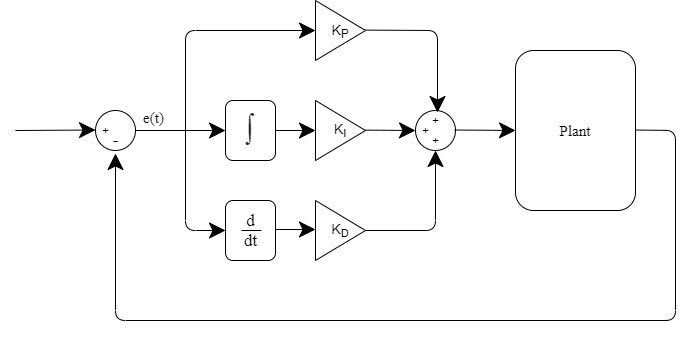
\includegraphics[width=\columnwidth]{PIDControl.png}%
	\caption{PID control block diagram.}%
	\label{fig:PIDControl}%
\end{figure}

PID control is comparatively simple compared to other techniques, but several studies suggest that it is generally effective for stabilising a UAV around a hovering setpoint, in the absence of large disturbances \cite{Bouabdallah2006}, \cite{Pounds2010}, \cite{Moussid2015}. \\

\subsection{Backstepping Control}\label{section:BacksteppingBackground}
The plant dynamics of a multi-rotor vehicle are inherently nonlinear, therefore nonlinear control techniques may be necessary to stabilise the vehicle. Backstepping control is a nonlinear recursive technique which is based upon Lyapunov stability. The mathematical background on the backstepping method in this section is largely based upon the work presented by Kokotovic \cite{1992a} and Krsti\'c et al. \cite{Krstic1995}.

\subsubsection{Lyapunov Stability}
Direct Lyapunov theorem, as stated in Appendix B of \cite{Isidori1995}, considers a time invariant system of the form:
\[\dot{x}=f(x)\]
with $x\in\mathbb{R}^{n}$, $f(x)$ is smooth and $f(0)=0$. If there exists a positive definite, proper and smooth function $V(x)$ which satisifies:
\[\frac{\partial V}{\partial x}f(x)<0\]
for all $x\neq0$, then the equilibrium of the system is globally asymptotically stable. This means that given any initial conditions, over time ($t\rightarrow\infty$) the system will approach its equilibrium point \cite{Chen1999}. 

Now, consider a time invariant nonlinear system with states $\mathbf{x}$ and inputs $\mathbf{u}$:
\begin{equation}\label{eqn:TISystem}
\mathbf{\dot{x}}=\mathbf{f}(\mathbf{x},\mathbf{u})
\end{equation}
with equilibrium at $\mathbf{x}=\mathbf{0}$. Following from Direct Lyapunov theorem, to stabilise such a system, a control law $\mathbf{u}=\mathbf{\alpha}(\mathbf{x})$ must be designed such that the equilibrium point of \eqref{eqn:TISystem} is globally asymptotically stable. To do this, a function $V(\mathbf{x})$ may be chosen as a candidate Lyapunov function. The control input, $\mathbf{\alpha}(\mathbf{x})$, must then be chosen such that $\dot{V}(\mathbf{x})=\frac{\partial V}{\partial \mathbf{x}}\mathbf{f}(\mathbf{x},\mathbf{\alpha}(\mathbf{x}))$ is negative definite for all $\mathbf{x}$. 

In order to apply this method to the tracking problem, the states of the system may be redefined as $\mathbf{z}=\mathbf{x}_{d}-\mathbf{x}$, where $\mathbf{x}_{d}$ represents the desired value of the states.

\subsubsection{Strict Feedback Form}
Backstepping control is best demonstrated on a system in strict feedback form \cite{1992a}. Consider the system:
\begin{equation*}
\begin{split}
\dot{x}_{1}&=f_{1}(x_{1},x_{2})\\
\dot{x}_{2}&=x_{3}+f_{2}(x_{1},x_{2})\\
\dot{x}_{3}&=u +f_{3}(x_{1},x_{2}, x_{3})
\end{split}
\end{equation*}

Now consider that $x_{2}$ can be used as a "virtual control" to stabilise $\dot{x}_{1}$, by choosing an appropriate Lyapunov function $V_{1}(x_{1})$. We will denote the virtual control (or desired value of the state) with a subscript 'd', e.g. $x_{2d}(x_{1})$ denotes the desired value of $x_{2}$. It is worth noting that although this is a function of $x_{1}$, it will henceforth be written as $x_{2d}$ for simplicity. Likewise for other virtual controls.  Now consider the error between the desired and actual values: $z_{2}=x_{2}-x_{2d}$. As we are considering the stabilisation problem, $x_{1d}=0$ and therefore $z_{1}=x_{1}$. To stabilise $z_{1}$, the virtual control $x_{2d}$ must be chosen such that the Lyapunov function $V_{1}(z_{1})$ has a negative time derivative.

Likewise, $x_{3}$ may be used to stabilise $z_{2}$ with a virtual control ($x_{3d}(z_{1},z_{2})$). A third error term is defined: $z_{3}=x_{3}-x_{3d}$. Also, a second Lyapunov function is defined: 
\begin{equation*}
V_{2}(z_{1},z_{2})=V_{1}(z_{1})+\frac{1}{2}z_{2}^{2}
\end{equation*}
The feedback law $x_{3d}$ is chosen such that the time derivative of this Lyapunov function is negative. 

The final iteration for this system is complete by choosing the actual control $u$ to stabilise $z_{3}$. Again, this is done in the same way by defining a third Lyapunov function:
\begin{equation*}
V_{3}(z_{1},z_{2},z_{3})=V_{2}(z_{1},z_{2})+\frac{1}{2}z_{3}^{2}
\end{equation*}
The control input $u$ is then chosen such that the time derivative is negative definite. This results in global asymptotic stability of the system at the equilibrium point. Thus the entire system is stabilised by the single control input ($u$) by the recursive backstepping of virtual control inputs ($x_{2d}$, $x_{3d}$). This concept is able to be applied to control the position of multi-rotor aircraft, by using the Euler angle values as virtual controls.


\subsubsection{Implementation in UAV Control}

A large number of studies have investigated various implementations of backstepping control strategies both in simulation and on physical UAV platforms. This control method is flexible and variations on the control law will arise depending on the design decision to cancel or retain nonlinearities. Also, the specific UAV platform and the modelling method used to describe the system can result in differences between the derived control laws.

Backstepping control systems for multi-rotor UAVs are simulated with successful results in many studies. \cite{Mian2008} demonstrates stabilisation of the rotational subsystem of a quadrotor using a backstepping control law, with the translational subsystem controlled using PID. \cite{ArellanoMuro2013} demonstrates satisfactory simulation results for trajectory tracking of a quadrotor in the presence of external disturbances. \cite{Roza2012} presents similar results with a controller that allows a speed profile and yaw angle to be specified as a function of displacement along the path. A backstepping controller is found to perform better in the presence of wind as compared to sliding mode control in \cite{Moussid2015}. Other studies which show robust simulated results for backstepping controllers include \cite{Madani2006}, \cite{XuanMung2019} and \cite{Shao2018}.

Further, multiple studies show good performance of backstepping controllers implemented on hardware platforms. \cite{Madani2006a} implements backstepping control on a UAV hardware platform on a test stand to demonstrate control of the yaw angle and z position only. \cite{Bouabdallah2006} demonstrates the use of backstepping with integral action for controlling a quadrotor UAV's attitude and position autonomously during indoor flights. Further research is required to demonstrate robust autonomous control in the presence of physical (rather than simulated) wind and external disturbances. 



\section{State Estimation}

%Address the different techniques and evaluate their use in previous studies
%Kalman Filter...
%Extended Kalman Filter...
%EKF is similar to KF, but linearises a nonlinear system about the current estimated trajectory.

%UKF...


%Sensor Fusion/Multi-rate/Redundancy/fault detection
To implement a stable control system, it is essential to have an accurate method of estimating the system states which the controller uses. There are many different types of sensors which can be used to gather data describing a vehicle's position, velocity, attitude and angular rates. A state estimation algorithm combines this data to reach a reasonable approximation of the system states. Common sensor fusion techniques include complementary filters, neural network-based algorithms and Kalman filter-based algorithms. 

The Kalman filter (also known as linear quadratic estimator) is a recursive algorithm which uses measurement data whilst accounting for noise to estimate unknown variables. The standard Kalman filter is the optimal filter for linear systems that are well characterised by the established model. However, there are two main Kalman filter-based techniques which have been adapted for nonlinear systems - the extended Kalman filter (EKF) and the unscented Kalman filter (UKF). Both algorithms are similar however the UKF applies an unscented transformation to propagate the random variables throughout the algorithm \cite{Wana}. However, \cite{StPierre} shows that the UKF is more computationally expensive than the EKF for inertial navigation and also that in GPS denied conditions the UKF offers no benefit over the EKF. Therefore, the EKF algorithm will be explored in more detail in this thesis.
\subsection{Extended Kalman Filter}\label{section:EKFBackground}

The extended Kalman filter applies the same concepts as the standard Kalman filter, with the addition of iteratively linearising the system around the current state estimates. The linearisation is performed using first order Taylor series. There are two main steps to the EKF algorithm: predict and update.
The "predict" step first uses the state transition functions ($\textbf{\textit{f}}(\textbf{\textit{x}},\textbf{\textit{u}})$) with the previous state estimate ($\hat{\textbf{\textit{x}}}_{k-1}$) and the current input (\textbf{\textit{u}}) values. Then the covariance matrix (\textbf{\textit{P}}) is predicted using the Jacobian of the state transition function ($F$).

\begin{equation*}
\begin{split}
\hat{\textbf{\textit{x}}}_{k}^{-}&=\textbf{\textit{f}}(\hat{\textbf{\textit{x}}}_{k-1}, \textbf{\textit{u}}_{k})\\
\textbf{\textit{P}}_{k}^{-}&=\textbf{\textit{F}}_{k}\textbf{\textit{P}}_{k-1}\textbf{\textit{F}}_{k}^{T}+\textbf{\textit{Q}}_{k}
\end{split}
\end{equation*}
where $\textbf{\textit{Q}}_{k}$ represents the process noise covariance matrix. $\textbf{\textit{F}}_{k}$ represents the Jacobian of the state transition function evaluated at ($\hat{\textbf{\textit{x}}}_{k}^{-}$, $\textbf{\textit{u}}_{k}$). That is $\textbf{\textit{F}}_{k}=\frac{\partial \textbf{\textit{f}}}{\partial \textbf{\textit{x}}}|_{\hat{\textbf{\textit{x}}}_{k}^{-}, \textbf{\textit{ u}}_{k}}$ . The "-" superscript denotes the initial estimate from the predict step.


The "update" step uses these predictions and compares them with the sensor measurements to achieve more accurate estimates.

\begin{equation*}
\begin{split}
\textbf{\textit{K}}_{k}&=\textbf{\textit{P}}_{k}^{-}\textbf{\textit{H}}_{k}^{T}(\textbf{\textit{H}}_{k}\textbf{\textit{P}}_{k}^{-}\textbf{\textit{H}}_{k}^{T}+\textbf{\textit{R}}_{k})^{-1}\\
\hat{\textbf{\textit{x}}}_{k}&=\hat{\textbf{\textit{x}}}_{k}^{-}+\textbf{\textit{K}}_{k}\left[\textbf{\textit{z}}_{k}-\textbf{\textit{h}}(\hat{\textbf{\textit{x}}}_{k}^{-})\right]\\
\textbf{\textit{P}}_{k}&=(\textbf{\textit{I}}-\textbf{\textit{K}}_{k}\textbf{\textit{H}}_{k})\textbf{\textit{P}}_{k}^{-}
\end{split}
\end{equation*}
where $\textbf{\textit{z}}_{k}$ represents the sensor measurements, $\textbf{\textit{h}}(\cdot)$ represents the measurement functions and \textbf{\textit{I}} represents an identity matrix. $\textbf{\textit{H}}_{k}$ represents the Jacobian of the measurement function evaluated at $\hat{\textbf{\textit{x}}}_{k}^{-}$. That is $\textbf{\textit{H}}_{k}=\frac{\partial \textbf{\textit{h}}}{\partial \textbf{\textit{x}}}|_{\hat{\textbf{\textit{x}}}_{k}^{-}}$.

\subsection{Magnetometer}
The Earth's magnetic field vector varies with latitude, longitude, altitude and time. In order to effectively utilise magnetometer data to determine true north it may be necessary to have knowledge of the magnetic field vector's expected value at a particular location. The International Geomagnetic Reference Field is a model of the Earth's magnetic field which is produced and updated by the International Association of Geomagnetism and Aeronomy (IAGA). This model allows a magnetic field vector to be estimated for any location on the globe and the magnetometer data will be compared to this reference to determine bearing in the sensor fusion algorithm. It is worth noting that many environments may have unpredictable magnetic fields caused by surrounding structures, machinery or other electrical equipment. For the purposes of state estimation it will be assumed that the measured magnetic field is representative of the Earth's magnetic field.

\subsection{Barometer}\label{section:barometerBackground}
Air pressure varies with altitude, which allows barometric pressure sensors to be used in the estimation of relative height. The U.S. National Aeronautics and Space Administration (NASA) have developed a standard atmospheric model \cite{Oceanic1976}. According to this model, pressure as a function of height above sea level can be found using \eqref{eqn:baroFormula}, when temperature lapse rate is zero. Temperature lapse rate describes the rate at which temperature changes with altitude. 

\begin{equation}\label{eqn:baroFormula}
P=P_{b}exp\left[\frac{-g M (H-H_{b})}{R T_{b}}\right]
\end{equation}
where $P_{b}$, $T_{b}$ and $H_{b}$ are the reference values of pressure, temperature and height respectively. The subscript b is representative of one of seven layers of the atmosphere. H is the height at which pressure is calculated, g is gravitational acceleration, M is the molar mass of air and R is the universal gas constant. 

Assuming the UAV operates at altitudes below 11 km above sea level, the subscript b is 0. Within this operating region the reference values are: $P_{0}=101 325$ Pascals, $T_{0}=288.15$ Kelvin and $H_{0}=0$ metres.

\subsection{GPS Denied Environments}
Most state estimation algorithms currently in use for UAV systems are dependent on GPS data for position estimation. However in many situations, GPS signal may be unavailable, practically disabling the UAV. To expand the operating region of the vehicle, it is necessary to have some form of position tracking algorithm which is able to accurately monitor position without GPS data. There are a number of techniques for achieving this including visual odometry and simultaneous localisation and mapping (SLAM) \cite{Balamurugan2016}. Complex systems will use a number of cameras, however a simple approach to visual odometry can be achieved by utilising a single optical flow sensor (OFS). An OFS is a camera which can be attached to the underside of a vehicle to record visual data of the surface. As the vehicle moves, the OFS captures and compares sequences of images to determine the motion of the vehicle. Using this data in combination with IMU data has been shown to be effective for state estimation \cite{Driessen2018}. 

\section{Chapter Summary}
This chapter has provided the technical background necessary for the development in the following chapters. A comprehensive review of current literature has also been established in order to reveal the more effective methods and the gaps in current research.



\clearpage




\chapter{Modelling of Multi-Rotor Aircraft}\label{chapter:Modelling}
\textit{In order to design a control system for an aircraft, a comprehensive mathematical model of the aircraft must first be defined. Within this chapter a complete state space representation is derived for a general multi-rotor vehicle. This is also extended to a specific vehicle configuration - the hexacopter. This final model is then simulated using Simulink to implement and validate the control methods in the following chapter.}

\section{General Multi-Rotor Model}\label{section:MultiRotorModel}
The initial model will be derived for a general multi-rotor vehicle using Newton-Euler formalism. This is done by considering the torque around each of the three axes and the total force produced by the propellers as the inputs to the system. This model can then be extended to most standard multi-rotor configurations by considering how the propellers generate these forces and torques in the configuration being considered.


\subsection{Reference Frames}
We will consider a vehicle in three-dimensional space with six degrees of freedom (DoF)- three translational DoF (x, y and z), and three rotational DoF (roll $\phi$, pitch $\theta$ and yaw $\psi$). For the derivation of this model, it is necessary to consider two reference frames: the Earth-fixed frame and the body-fixed frame. The Earth-fixed local frame is that which has its origin at an arbitrary, stationary point on the Earth's surface, while the body-fixed frame originates at the vehicle's centre of mass and travels with the vehicle \cite{Nebylov2016}. The Earth-fixed frame will be considered an inertial frame for the purposes of this model. Note that in order to maintain right-hand orthogonality the inertial frame is traditionally defined with the positive x axis pointing North, the positive y axis pointing East and the positive z axis pointing down towards the Earth (known as North-East-Down (NED) co-ordinates). The NED reference frame is represented in \figref{fig:RefFrames} a) with axes ($x_{n}$, $y_{n}$, $z_{n}$). For the purposes of modelling an aerial vehicle it is more intuitive to have the z axis positive in the upward direction (corresponding to vehicle altitude).Therefore, a second inertial frame will be defined with axes ($x=x_{n}$, $y=y_{n}$, $z=-z_{n}$) as shown in \figref{fig:RefFrames} b). This reference frame will be referred to as the Earth frame and will be the main coordinate system used throughout this thesis. The body frame is defined with its origin at the vehicle's centre of mass with the z axis opposite to the direction of propeller thrust. The input torques ($\tau_{\phi}$, $\tau_{\theta}$, $\tau_{\psi}$) are defined around the axes of the body frame ($x_{b}$, $y_{b}$, $z_{b}$) as depicted in \figref{fig:RefFrames} c).\\


\begin{figure}[htb]
	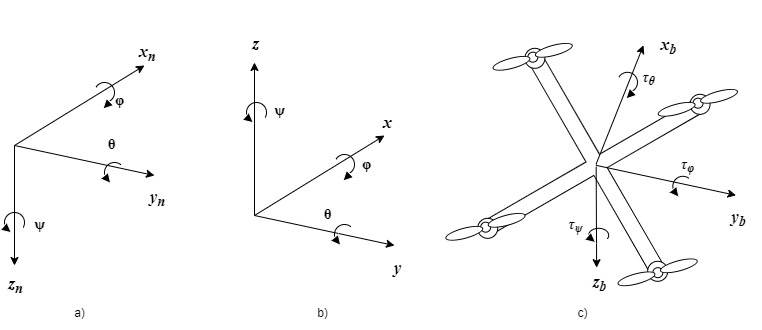
\includegraphics[width=\columnwidth]{RefFrames.jpg}%
	\caption{Reference frames and co-ordinate systems: a) NED Frame b) Earth Frame c) Body Frame}%
	\label{fig:RefFrames}%
\end{figure}

To transform linear quantities (displacement, velocity, acceleration) between the inertial NED coordinate system ($x_{n}, y_{n}, z_{n}$) and the body-fixed coordinate system ($x_{b}, y_{b}, z_{b}$) it is necessary to establish a rotation matrix ($C^{b}_{n}$) such that:
\[
\begin{bmatrix}
x_{b}\\ y_{b}\\ z_{b}
\end{bmatrix} = C^{b}_{n}\begin{bmatrix}
x_{n}\\ y_{n}\\ z_{n}
\end{bmatrix}
\]

To establish this matrix it is necessary to consider the rotation of the body-fixed frame around each of its axes \cite{Cook2013}. This is done by multiplying by three intermediate rotation matrices: $C^{b}_{n}(\phi)$, $C^{b}_{n}(\theta)$ and $C^{b}_{n}(\psi)$. Since matrix multiplication is not commutative, the order of these rotations is an important part of the model. The body frame is first rotated around the x axis (roll) by an angle $\phi$ to an intermediate reference frame: 
\[
\begin{bmatrix}
x_{b}\\ y_{b}\\ z_{b}
\end{bmatrix} = C^{b}_{n}(\phi)\begin{bmatrix}
x_{b_{1}}\\ y_{b_{1}}\\ z_{b_{1}}
\end{bmatrix}=
\begin{bmatrix}
1 & 0 & 0\\ 
0 & cos(\phi) & sin(\phi)\\ 
0 & -sin(\phi) & cos(\phi)
\end{bmatrix}
\begin{bmatrix}
x_{b_{1}}\\ y_{b_{1}}\\ z_{b_{1}}
\end{bmatrix}
\]
Rotating this set of coordinates around the y axis (pitch) will result in another intermediate reference frame:
\[
\begin{bmatrix}
x_{b_{1}}\\ y_{b_{1}}\\ z_{b_{1}}
\end{bmatrix} = C^{b}_{n}(\theta)\begin{bmatrix}
x_{b_{2}}\\ y_{b_{2}}\\ z_{b_{2}}
\end{bmatrix}=
\begin{bmatrix}
cos(\theta) & 0 & -sin(\theta)\\ 
0 & 1 & 0\\ 
sin(\theta) &  0 & cos(\theta)
\end{bmatrix}
\begin{bmatrix}
x_{b_{2}}\\ y_{b_{2}}\\ z_{b_{2}}
\end{bmatrix}
\]
Finally, this frame is rotated around the z axis (yaw):
\[
\begin{bmatrix}
x_{b_{2}}\\ y_{b_{2}}\\ z_{b_{2}}
\end{bmatrix} = C^{b}_{n}(\psi)\begin{bmatrix}
x_{n}\\ y_{n}\\ z_{n}\\
\end{bmatrix}=
\begin{bmatrix}
cos(\psi) & sin(\psi) & 0\\
-sin(\psi) & cos(\psi) & 0 \\ 
0 & 0 & 1\\ 
\end{bmatrix}
\begin{bmatrix}
x_{n}\\ y_{n}\\ z_{n}
\end{bmatrix}
\]
Therefore, via substitution, the multiplication of these three intermediate matrices gives the final rotation matrix- also commonly known as the Direction Cosine Matrix (DCM) \cite{Nebylov2016}:
\begin{align*}
C^{b}_{n} &= C^{b}_{n}(\phi)C^{b}_{n}(\theta)C^{b}_{n}(\psi)\\
&=\begin{bmatrix}
cos(\theta)cos(\psi) & cos(\theta)sin(\psi) & -sin(\theta)\\
sin(\phi)sin(\theta)cos(\psi)-cos(\phi)sin(\psi) & sin(\phi)sin(\theta)sin(\psi)+cos(\phi)cos(\psi) & sin(\phi)cos(\theta) \\ 
cos(\phi)sin(\theta)cos(\psi)+sin(\phi)sin(\psi) & cos(\phi)sin(\theta)sin(\psi)-sin(\phi)cos(\psi) & cos(\phi)cos(\theta)\\ 
\end{bmatrix}
\end{align*}


An important characteristic of this rotation matrix is its orthogonality, which implies its inverse is equal to its transpose i.e. $C^{n}_{b}=(C^{b}_{n})^{-1}= (C^{b}_{n})^{T}$.


\subsection{Model Dynamics}\label{section:ModelDynamics}
Standard configurations of multi-rotor vehicles consist of a number of propellers arranged symmetrically around the central body, all producing a force in the same direction. Therefore, regardless of the force produced by each individual propeller, the total thrust can only be produced in one direction which is aligned with the vehicle's vertical (z) axis. However, the differences in the forces produced by individual propellers will influence the rotational mechanics of the vehicle causing roll, pitch and yaw torques. 

This system is an under-actuated system, since there are six degrees of freedom (x, y, z, $\phi, \theta, \psi$) but only four effective inputs- the torque around each axis and the total thrust (\(\tau_{\phi},\tau_{\theta}, \tau_{\psi}, F_{T}\)). This means that it is not possible to directly affect two of the degrees of freedom. For example, assuming the body frame is initially aligned with the Earth frame, the two horizontal translational motions (x and y) can not be directly affected, as the thrust vector is aligned with the z axis. In order to cause translational motion in the x direction it is first necessary to change the pitch angle ($\theta$), which causes the thrust vector to have an x component. Likewise, to move in the y direction the roll angle ($\phi$) must first change.\\

To obtain the rates of change of the Euler angles ($\dot{\phi}$, $\dot{\theta}$, $\dot{\psi}$) from the angular velocities around the body-fixed axes (p, q, r), it is necessary to use the intermediate rotation matrices \cite{Nelson1997}.


\begin{align*}
\begin{bmatrix}
p\\q\\r
\end{bmatrix}
&= C^{b}_{n}(\phi)C^{b}_{n}(\theta)
\begin{bmatrix}
0\\0\\\dot{\psi}
\end{bmatrix}
+C^{b}_{n}(\phi)
\begin{bmatrix}
0\\\dot{\theta}\\0
\end{bmatrix}
+
\begin{bmatrix}
\dot{\phi}\\0\\0
\end{bmatrix}\\
&=
\begin{bmatrix}
1 & 0 & -sin(\theta)\\
0 & cos(\phi) & sin(\phi)cos(\theta)\\
0 & -sin(\phi) & cos(\phi)cos(\theta)
\end{bmatrix}
\begin{bmatrix}
\dot{\phi}\\ \dot{\theta} \\ \dot{\psi}
\end{bmatrix}\\
\end{align*}

Taking the inverse of this matrix gives a set of expression for the rates of change of the Euler angles. 
\begin{equation}\label{eqn:state1}
\begin{bmatrix}
\dot{\phi}\\ \dot{\theta} \\ \dot{\psi}
\end{bmatrix} 
=
\begin{bmatrix}
1 & sin(\phi)tan(\theta) & cos(\phi)tan(\theta)\\
0 & cos(\phi) & -sin(\phi)\\
0 & sin(\phi)sec(\theta) & cos(\phi)sec(\theta)
\end{bmatrix}
\begin{bmatrix}
p\\q\\r
\end{bmatrix} 
\end{equation}


Next, the Newton-Euler equations of motion will be explored with respect to the body-fixed frame linear velocities (u, v, w) and angular velocities (p, q, r).
\begin{equation}\label{eqn:NewtEul1}
F=m\left(
\begin{bmatrix}
\dot{u}\\\dot{v}\\\dot{w}
\end{bmatrix}
+
\begin{bmatrix}
p\\q\\r
\end{bmatrix}
\times
\begin{bmatrix}
u\\v\\w
\end{bmatrix}
\right)
\end{equation}



For now it will be assumed the only forces acting on the vehicle are the vehicle's weight (in the positive direction of the NED frame z axis) and the total thrust produced by the propellers (in the negative direction of the body-fixed z axis). Substituting these forces into Equation \eqref{eqn:NewtEul1} and rearranging gives:
\begin{equation}\label{eqn:state2}
\begin{bmatrix}
\dot{u}\\\dot{v}\\\dot{w}
\end{bmatrix}
= 
\begin{bmatrix}
rv-qw-gsin(\theta)\\
pw-ru+gsin(\phi)cos(\theta)\\
qu-pv+gcos(\phi)cos(\theta)-\frac{1}{m}F_{T}
\end{bmatrix}
\end{equation}

Next, the rotational motion is considered:
\[
\begin{bmatrix}
\tau_{\phi}\\\tau_{\theta}\\\tau_{\psi}
\end{bmatrix}
=I_{b}
\begin{bmatrix}
\dot{p}\\\dot{q}\\\dot{r}
\end{bmatrix}
+ \begin{bmatrix}
p\\q\\r
\end{bmatrix}
\times
I_{b}
\begin{bmatrix}
p\\q\\r
\end{bmatrix}
\]
Where $I_{b}$ represents the vehicle's moment of inertia matrix. Assuming that the vehicle is symmetric about its axes, $I_{b}$ will be a diagonal matrix:
\[I_{b}=
\begin{bmatrix}
I_{xx} & 0 & 0\\
0 & I_{yy} & 0\\
0 & 0 & I_{zz}
\end{bmatrix}
\]
Rearranging for the derivatives of the angular velocities gives:
\begin{equation}\label{eqn:state3}
\begin{bmatrix}
\dot{p}\\\dot{q}\\\dot{r}
\end{bmatrix}
=
\begin{bmatrix}
\frac{I_{yy}-I_{zz}}{I_{xx}}qr+\frac{1}{I_{xx}}\tau_{\phi}\\
\frac{I_{zz}-I_{xx}}{I_{yy}}pr+\frac{1}{I_{yy}}\tau_{\theta}\\
\frac{I_{xx}-I_{yy}}{I_{zz}}pq+\frac{1}{I_{zz}}\tau_{\psi}
\end{bmatrix}
\end{equation}



Finally, it will be necessary to obtain the position of the vehicle with respect to the Earth reference frame. Therefore, the derivatives of the NED frame $x_{n}$, $y_{n}$ and $z_{n}$ positions are obtained by multiplying the rotational matrix $C^{n}_{b}$ by the body-fixed frame linear velocities (u, v and w). This gives \eqref{eqn:NEDvel}, with c($\bullet$) and s($\bullet$) representing cos($\bullet$) and sin($\bullet$) respectively. 
\begin{equation}\label{eqn:NEDvel}
\begin{bmatrix}
\dot{x}_{n}\\\dot{y}_{n}\\\dot{z}_{n}
\end{bmatrix}
=
\begin{bmatrix}
c(\theta)c(\psi) & s(\phi)s(\theta)c(\psi)-c(\phi)s(\psi) & c(\phi)s(\theta)c(\psi)+s(\phi)s(\psi)\\
c(\theta)s(\psi) & s(\phi)s(\theta)s(\psi)+c(\phi)c(\psi) & c(\phi)s(\theta)s(\psi)-s(\phi)c(\psi)\\
-s(\theta) & s(\phi)c(\theta) & c(\phi)c(\theta)
\end{bmatrix}
\begin{bmatrix}
u\\v\\w
\end{bmatrix}
\end{equation}

These velocities can then be converted into the Earth frame with the z axis pointing up, as shown in \eqref{eqn:state4}.
\begin{small}
\begin{equation}\label{eqn:state4}
\begin{bmatrix}
\dot{x}\\\dot{y}\\\dot{z}
\end{bmatrix}
=
\begin{bmatrix}
\dot{x}_{n}\\\dot{y}_{n}\\-\dot{z}_{n}
\end{bmatrix}
=
\begin{bmatrix}
c(\theta)c(\psi) & s(\phi)s(\theta)c(\psi)-c(\phi)s(\psi) & c(\phi)s(\theta)c(\psi)+s(\phi)s(\psi)\\
c(\theta)s(\psi) & s(\phi)s(\theta)s(\psi)+c(\phi)c(\psi) & c(\phi)s(\theta)s(\psi)-s(\phi)c(\psi)\\
s(\theta) & -s(\phi)c(\theta) & -c(\phi)c(\theta)
\end{bmatrix}
\begin{bmatrix}
u\\v\\w
\end{bmatrix}
\end{equation}
\end{small}

\eqref{eqn:state1}, (\ref{eqn:state2}), (\ref{eqn:state3}) and (\ref{eqn:state4}) comprise a complete state space model describing a general multi-rotor vehicle with 12 states. This state space model will be used for simulation of the multi-rotor.

It is important to note that although this model does not make any approximations, it does not necessarily consider every force the vehicle may be subject to. For example, the effects of wind, air friction and gyroscopic effects have not been considered in this model for simplicity. Also the dynamics of the motors and propellers have not yet been considered, since the torques and total force were chosen as the inputs.

\FloatBarrier
\subsection{Additional Translational Motion Equations}\label{section:AddTransMotion}
Although the model defined in Section \ref{section:ModelDynamics} is a complete state space model for the system, the translational motion is able to be represented in another form which will be useful for controllers defined in the following chapter. 
The only forces acting on the vehicle are gravity - in the Earth frame negative z direction- and the total thrust - in the body frame negative z direction. This is expressed in \eqref{eqn:additionalState1}
\begin{equation}\label{eqn:additionalState1}
\begin{split}
F&=
\begin{bmatrix}
0\\0\\-mg
\end{bmatrix}
+
\begin{bmatrix}
c(\theta)c(\psi) & s(\phi)s(\theta)c(\psi)-c(\phi)s(\psi) & c(\phi)s(\theta)c(\psi)+s(\phi)s(\psi)\\
c(\theta)s(\psi) & s(\phi)s(\theta)s(\psi)+c(\phi)c(\psi) & c(\phi)s(\theta)s(\psi)-s(\phi)c(\psi)\\
s(\theta) & -s(\phi)c(\theta) & -c(\phi)c(\theta)
\end{bmatrix}
\begin{bmatrix}
0\\0\\-F_{T}
\end{bmatrix}\\
&=
\begin{bmatrix}
(-c(\phi)s(\theta)c(\psi)-s(\phi)s(\psi))F_{T}\\
(-c(\phi)s(\theta)s(\psi)+s(\phi)c(\psi))F_{T}\\
c(\phi)c(\theta)F_{T}-mg
\end{bmatrix}
\end{split}
\end{equation}

Using Newton's second law of motion ($F=ma$) in the Earth frame gives the second order differential equations in \eqref{eqn:additionalState2}.\\
\begin{equation}\label{eqn:additionalState2}
\begin{bmatrix}
\ddot{x}\\\ddot{y}\\\ddot{z}
\end{bmatrix}
=
\begin{bmatrix}
(-c(\phi)s(\theta)c(\psi)-s(\phi)s(\psi))\frac{F_{T}}{m}\\
(-c(\phi)s(\theta)s(\psi)+s(\phi)c(\psi))\frac{F_{T}}{m}\\
c(\phi)c(\theta)\frac{F_{T}}{m}-g
\end{bmatrix}
\end{equation}

\section{Hexacopter Model}
To extend the general multi-rotor model to a hexacopter, the six propeller forces need to be converted to the general model's inputs: three torques (around each axis) and one force (describing the total thrust). To achieve this, the configuration of the hexacopter must be defined. \figref{fig:hex} shows the basic geometry of a hexacopter platform with \(P_{1}, P_{2},...,P_{6}\) representing the six propellers. 

\begin{figure}[htb]
\begin{center}
	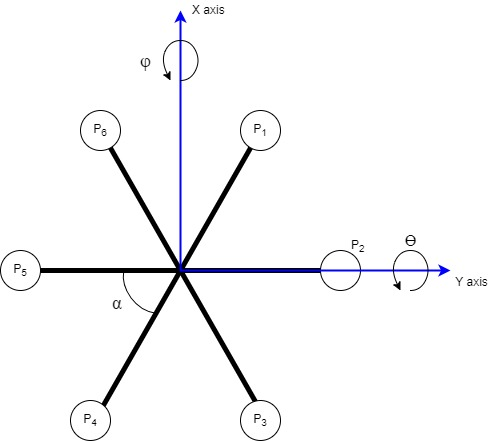
\includegraphics[width=90mm]{HexacopterConfig.jpg}%
	\end{center}
	\caption{Basic configuration of the hexacopter with labelled axes.}%
	\label{fig:hex}%
\end{figure}


Let \(F_{1}, F_{2},...,F_{6}\) denote the force produced by each of the propellers as numbered in \figref{fig:hex}. The torques around each axis are proportional to the distance of each propeller from the axis. Using the geometry of the hexacopter, the torques around each axis can be derived.
\begin{flushleft}
\[\tau_{\phi}=d[(F_{5}-F_{2})+\cos(\alpha)(F_{6}+F_{4}-F_{1}-F_{3})]\]\\
\[\tau_{\theta}=d\sin(\alpha)(F_{1}-F_{3}-F_{4}+F_{6})\]\\
\[\tau_{\psi}=K_{R}(F_{1}-F_{2}+F_{3}-F_{4}+F_{5}-F_{6})\]
\end{flushleft}
Where d represents the distance from each propeller to the hexacopter's centre of mass, \(\alpha\) represents the angle between each of the arms and $K_{R}$ represents a constant arising from the reaction force on the propellers. In this case, the angles between each of the arms will be considered to be equal, therefore \(\alpha\) is 60\(^{\circ}\). This matches the configuration of the hardware platform discussed in Chapter \ref{chapter:Implementation}. It follows that \(\sin(\alpha)=\frac{\sqrt{3}}{2}\) and \(\cos(\alpha)=\frac{1}{2}\)\\

Next, it is necessary to express the torques in terms of the speed of the propellers. The force produced by the propellers is approximately proportional to the square of the speed of the propellers (\(\Omega_{i}^{2}\)). For now it is sufficient to relate the quantities with a constant (\(C_{T}\)) which is known to be related to the physical properties of the propeller and the medium in which it is rotating. These quantities are related by a different constant when considering the yaw torque (\(\tau_{\psi}\)) since this torque arises from reaction forces. The proportionality between the square of the propeller speeds and yaw torque will be represented by \(K_{\psi}\). The total thrust produced by the propellers (\(F_{T}\)) is simply the sum of the forces produced by each propeller. The relationship between the propeller speeds and input torques and force can thus be expressed in matrix form as in \eqref{eqn:propSpeeds1}.

\begin{equation}\label{eqn:propSpeeds1}
\begin{bmatrix}
\tau_{\phi}\\
\tau_{\theta}\\
\tau_{\psi}\\
F_{T}\\
\end{bmatrix}
=
\begin{bmatrix}
-\frac{C_{T}d}{2} & -C_{T}d & -\frac{C_{T}d}{2} & \frac{C_{T}d}{2} & C_{T}d & \frac{C_{T}d}{2}\\
    \frac{C_{T}d\sqrt{3}}{2} & 0 & -\frac{C_{T}d\sqrt{3}}{2} & -\frac{C_{T}d\sqrt{3}}{2} & 0 & \frac{C_{T}d\sqrt{3}}{2}\\
    K_{\psi} & -K_{\psi} & K_{\psi} & -K_{\psi} & K_{\psi} & -K_{\psi}\\
    C_{T} & C_{T} & C_{T} & C_{T} & C_{T} & C_{T}
\end{bmatrix}
\begin{bmatrix}
\Omega^{2}_{1}\\
\Omega^{2}_{2}\\
\Omega^{2}_{3}\\
\Omega^{2}_{4}\\
\Omega^{2}_{5}\\
\Omega^{2}_{6}\\
\end{bmatrix}
\end{equation}

It is also necessary to consider actuator saturation as part of this model. The motors which drive the propellers are limited in that they can only spin in a single direction and have a maximum speed output. That is, motor speeds $(\Omega_{1},\Omega_{2},\Omega_{3},\Omega_{4},\Omega_{5},\Omega_{6})$ are restricted such that:
\begin{equation}\label{eqn:saturation}
sat(\Omega_{i})=\begin{cases}
      \Omega_{max}, & \Omega_{i}>\Omega_{max}\\
      \Omega_{i}, & 0\leq\Omega_{i}\leq\Omega_{max}\\
      0, & \Omega_{i}<0
    \end{cases} 
\end{equation}
The block diagram of the final hexacopter model which combines \eqref{eqn:state1}, (\ref{eqn:state2}), (\ref{eqn:state3}), (\ref{eqn:state4}), (\ref{eqn:propSpeeds1}) and (\ref{eqn:saturation}) is shown in \figref{fig:FinalModel}.
\begin{figure}[htb]
\begin{center}
	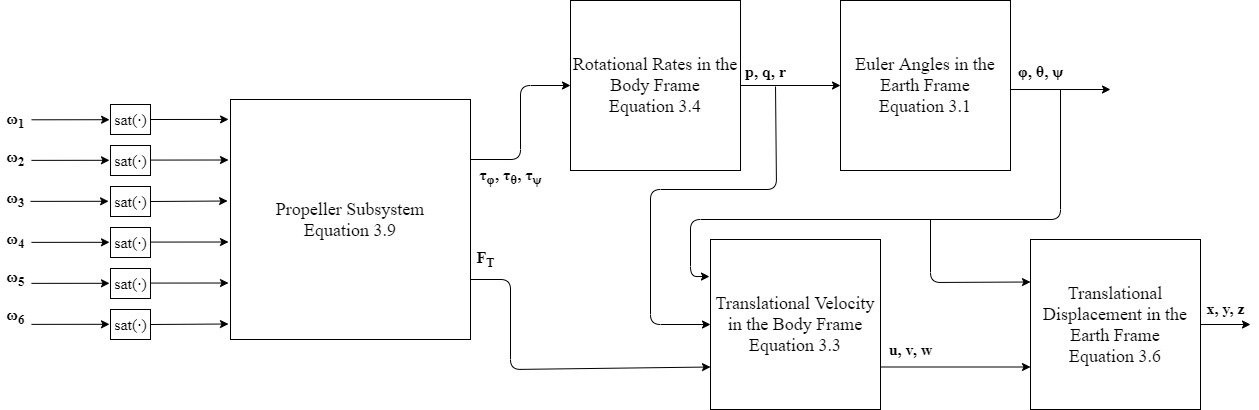
\includegraphics[width=\columnwidth]{ModelBlockDiagram.jpg}%
	\end{center}
	\caption{Hexacopter model block diagram.}%
	\label{fig:FinalModel}%
\end{figure}

 
\section{Simulation}
The model derived in the previous section is simulated using Simulink. The block diagrams created within Simulink are shown in Appendix \ref{section:Simu_Plant}.

The intent is to simulate the physical vehicle described in Section \ref{section:Hardware}. The vehicle's geometry and mass were measured, and are shown in \tabref{table:parameters} along with the other parameters used in the model. The maximum propeller speed was estimated based upon the voltage supplied by the battery and the manufacturer specifications. The propeller thrust coefficient was estimated, based upon the vehicles mass and the motors maximum speed. Since the vehicle is able to accelerate vertically, the thrust produced by the propellers must overcome the weight force, i.e. $C_{T}\Omega_{max}^{2}>mg$. Since more accurate methods were not readily available, a reasonable value of $C_{T}$ that satisfies this relationship was chosen. The yaw reaction torque coefficient was chosen to have the same order of magnitude as \cite{Bouabdallah2006} and \cite{Tayebi2004}. The moments of inertia around each axis are those measured for a similarly sized hexacopter using a pendulum by Capello et al. \cite{Capello2015}. These parameters do not exactly characterise the physical platform that is to be used, however the problem of parameter uncertainty is addressed in Section \ref{section:IntBack}.

\begin{table}[htb]\label{table:parameters}
\begin{center}
\begin{tabular}{||c|c|c|c||} 
 \hline
 Model Parameter & Symbol & Value & Units \\ [0.5ex] 
 \hline\hline
 Acceleration due to gravity & g & 9.81 & m s\textsuperscript{-2} \\ 
 \hline
 Vehicle mass & m & 1.404 & kg  \\
 \hline
 Moment of inertia (x) & I\textsubscript{xx} & 0.0286 & kg m\textsuperscript{2}\\
\hline
Moment of inertia (y) & I\textsubscript{yy} & 0.0254 & kg m\textsuperscript{2}\\
\hline
Moment of inertia (z) & I\textsubscript{zz} & 0.0418  & kg m\textsuperscript{2}\\
 \hline
 Angle between rotor arms & $\alpha$ & 60 & \textdegree\\
 \hline
 Maximum propeller speed & $\Omega_{max}$ & 252 & rev s\textsuperscript{-1}\\
 \hline
 Propeller thrust coefficient & $C_{T}$ & $4.5\times10^{-5}$ & N s\textsuperscript{2}\\
 \hline
 Yaw reaction torque coefficient & $K_{\phi}$ & $1.00\times10^{-7}$& N m s\textsuperscript{2}\\
\hline
 Distance from centre of gravity to propeller & d& 0.217 & m \\ [1ex] 
 \hline
\end{tabular}
\caption{Model simulation parameters}
\end{center}
\end{table}
 






\FloatBarrier
\section{Chapter Summary}
Within this chapter a complete state space representation has been derived to describe the dynamics of a general multi-rotor vehicle. This model has then been extended to a specific six rotor vehicle configuration. The simulation of the established model has been developed using Simulink. This simulated model will enable verification and testing of the control systems which are developed in the following chapter.
\clearpage




\chapter{Control of Multi-Rotor Aircraft}

\textit{Now that a sufficiently accurate mathematical model of the hexacopter has been developed, the control problem is able to be approached. Within this chapter two control systems will be developed with the aim of controlling the aircraft position and attitude. Simulations will then be performed in Simulink to verify the effectiveness of each control system. For the purposes of these simulations it will be assumed that the vehicle's position and attitude (x, y, z, $\phi$, $\theta$, $\psi$) can be accurately measured at any given time.} 

\section{Pseudo-inverse of Motor Speed Matrix}
The control systems in this chapter will be based upon the effective inputs of the plant i.e. $\tau_{\phi}$, $\tau_{\theta}$, $\tau_{\psi}$, $F_{T}$. Therefore, it will be necessary to implement an inverse of the matrix in Equation \ref{eqn:propSpeeds1} in order to obtain the desired input motor speeds. This matrix is not square and is therefore not invertible. However, for a matrix A with linearly independent rows, the Penrose-Moore pseudo-inverse ($A^{+}$) is able to be computed such  that: 
\[A^{+}= A^{T}(AA^{T})^{-1}\]
In this case, this is a right inverse which will satisfy \(AA^{+}=I\) where I is an identity matrix. The pseudo-inverse matrix is shown in Equation \ref{eqn:propSpeeds2} and will be used to reverse the relationship between the effective inputs and the propeller speeds.
\begin{equation}\label{eqn:propSpeeds2}
\begin{bmatrix}
\Omega^{2}_{1}\\
\Omega^{2}_{2}\\
\Omega^{2}_{3}\\
\Omega^{2}_{4}\\
\Omega^{2}_{5}\\
\Omega^{2}_{6}\\
\end{bmatrix}
=
\begin{bmatrix}
-\frac{1}{6C_{T}d} & \frac{\sqrt{3}}{(6C_{T}d)} &  \frac{1}{6K_{psi}} & \frac{1}{6C_{T}}\\
-\frac{1}{3C_{T}d} & 0 & -\frac{1}{6K_{psi}} & \frac{1}{6C_{T}}\\
-\frac{1}{6C_{T}d} & -\frac{\sqrt{3}}{(6C_{T}d)} & \frac{1}{6K_{psi}} & \frac{1}{6C_{T}}\\
 \frac{1}{6C_{T}d} & -\frac{\sqrt{3}}{(6C_{T}d)} & -\frac{1}{6K_{psi}} & \frac{1}{6C_{T}}\\
 \frac{1}{3C_{T}d} & 0 & \frac{1}{6K_{psi}} & \frac{1}{6C_{T}}\\
 \frac{1}{6C_{T}d} &  \frac{\sqrt{3}}{(6C_{T}d)} & -\frac{1}{6K_{psi}} & \frac{1}{6C_{T}}
\end{bmatrix}
\begin{bmatrix}
\tau_{\phi}\\
\tau_{\theta}\\
\tau_{\psi}\\
F_{T}\\
\end{bmatrix}
\end{equation}

\section{PID Control}
Initially, a control strategy for the hexacopter will be developed based upon Proportional Integral Derivative (PID) control. The basic concept of PID control is outlined in Section \ref{section:PIDBackground}. This controller will be designed with the aim of stabilising the vehicle around a hovering point and this allows the model to be simplified.
\subsection{Simplified Model}\label{section:SimpleModel}
For the purposes of this controller, the vehicle will assumed to be hovering, which implies the roll and pitch angles ($\phi$ $\theta$) will only have small variations from the origin. These assumptions will be used in developing the controller, however the controller will be verified by simulation on the full nonlinear model. Likewise, we will assume the yaw angle ($\psi$) is held close to the origin. This allows the small angle approximation to be applied to the model defined in Section \ref{section:ModelDynamics}. Applying this assumption to Equation \ref{eqn:state1} gives Equation \ref{eqn:simpleState1}.

\begin{equation}\label{eqn:simpleState1}
\begin{split}
\begin{bmatrix}
\dot{\phi}\\ \dot{\theta} \\ \dot{\psi}
\end{bmatrix} 
&=
\begin{bmatrix}
1 & 0 & 0\\
0 & 1 & 0\\
0 & 0 & 1
\end{bmatrix}
\begin{bmatrix}
p\\q\\r
\end{bmatrix} \\
\begin{bmatrix}
\dot{\phi}\\ \dot{\theta} \\ \dot{\psi}
\end{bmatrix} 
&=
\begin{bmatrix}
p\\q\\r
\end{bmatrix}
\end{split}
\end{equation} 




Likewise, it will be assumed that the moments of inertia around each axis are approximately equal ($I_{xx}\approx I_{yy}\approx I_{zz}$). Using this assumption and the relationship in Equation \ref{eqn:simpleState1}, Equation \ref{eqn:state3} can be simplified to give Equation \ref{eqn:simpleState3}. This allows the rotational systems to be decoupled and therefore more easily controlled using the PID technique.
\begin{equation}\label{eqn:simpleState3}
\begin{bmatrix}
\ddot{\phi}\\\ddot{\theta}\\\ddot{\psi}
\end{bmatrix}
=
\begin{bmatrix}
\frac{1}{I_{xx}}\tau_{\phi}\\
\frac{1}{I_{yy}}\tau_{\theta}\\
\frac{1}{I_{zz}}\tau_{\psi}
\end{bmatrix}
\end{equation}


Further, by applying the small angle approximation to \eqref{eqn:additionalState2}, the translational motion is able to be linearised. This is shown in Equation \eqref{eqn:simpleTranslational}.
\begin{equation}\label{eqn:simpleTranslational}
\begin{bmatrix}
\ddot{x}\\\ddot{y}\\\ddot{z}
\end{bmatrix}
=
\begin{bmatrix}
-\theta\frac{F_{T}}{m}\\
\phi\frac{F_{T}}{m}\\
\frac{F_{T}}{m}-g
\end{bmatrix}
\end{equation}

Under these assumptions, each Euler angle is directly controllable by the corresponding torque input,  vertical translational motion is controllable by the total thrust and horizontal translational motion is controllable by the roll and pitch angles. Additionally, from Equations \ref{eqn:simpleState3} and \ref{eqn:simpleTranslational}, it is apparent that there are double integrators in the plant dynamics\cite{Herzog2016}. Therefore, the integral term usually present in PID controllers will be unnecessary, i.e. the controllers designed in this section will use a PD structure.

\FloatBarrier
\subsection{Attitude Control}
In order to control the orientation of the vehicle, a PD control system is used for each angle. The torque around each axis is used to control the corresponding angles. The PD control laws for each torque input are defined in Equation \ref{eqn:torquePD}.

\begin{equation}\label{eqn:torquePD}
\begin{bmatrix}
\tau_{\phi}\\\tau_{\theta}\\\tau_{\psi}
\end{bmatrix}
=
\begin{bmatrix}
K_{P_{\phi}}(\phi_{d}-\phi)+K_{D_{\phi}}(\dot{\phi_{d}}-\dot{\phi})\\
K_{P_{\theta}}(\theta_{d}-\theta)+K_{D_{\theta}}(\dot{\theta_{d}}-\dot{\theta})\\
K_{P_{\psi}}(\psi_{d}-\psi)+K_{D_{\psi}}(\dot{\psi_{d}}-\dot{\psi})
\end{bmatrix}
\end{equation}
Where K coefficients represent non-negative constants and $\phi_{d}$, $\theta_{d}$ and $\psi_{d}$ represent the desired attitude of the vehicle.


\FloatBarrier
\subsection{Altitude Control}
From \eqref{eqn:additionalState2}, the relationship between the total thrust and acceleration in the z direction is given by: $F_T= \frac{m}{cos(\theta)cos(\phi)}(\ddot{z}+g)$. Using this, the control law for z can be defined as shown in \eqref{eqn:altitudePID}.
\begin{equation}\label{eqn:altitudePID}
F_{T}=\frac{m}{cos(\theta)cos(\phi)}[K_{P_{z}}(z_{d}-z)+K_{D_{z}}(\dot{z}_{d}-\dot{z})+g]
\end{equation}
Where K coefficients represent non-negative constants and $z_{d}$ represents the desired altitude.
 
\FloatBarrier
\subsection{Position Control}
Finally, the x and y position must be controlled to prevent the vehicle from drifting from its setpoint in the presence of disturbances, e.g wind gusts. This system should also allow the vehicle to travel to a specified coordinate within the Earth frame. Since the lateral and longitudinal motion of the vehicle cannot be directly controlled, the position is controlled by adjusting the desired values of the roll and pitch angles ($\phi_{d}$, $\theta_{d}$).
The relationship between x,y, $\phi$ and $\theta$ is linearised in Equation \ref{eqn:simpleTranslational}. Further, since the vehicle is assumed to be hovering, the thrust force must counter the vehicle's weight i.e. $F_{T}\approx mg \Rightarrow \frac{F_{T}}{m}\approx g$. 

\[\phi=\frac{1}{g}\ddot{y}\]
\[\theta=-\frac{1}{g}\ddot{x}\]

Using this linearised relationship, two PD controllers (scaled by $\pm\frac{1}{g}$) can be designed to take the position error as an input and will output the desired roll and pitch angles. These control laws are represented in Equation \ref{eqn:positionPD}
\begin{equation}\label{eqn:positionPD}
\begin{bmatrix}
\phi_{d}\\\theta_{d}
\end{bmatrix}
=
\begin{bmatrix}
\frac{1}{g}[K_{P_{y}}(y_{d}-y)+K_{D_{y}}(\dot{y_{d}}-\dot{y})]\\
-\frac{1}{g}[K_{P_{x}}(x_{d}-x)+K_{D_{x}}(\dot{x_{d}}-\dot{x})]
\end{bmatrix}
\end{equation}
Where K coefficients represent non-negative constants, $x_{d}$ and $y_{d}$ represent the desired horizontal position in the Earth frame. This controller is added in an outer loop with its outputs being supplied to the attitude controller. 

\FloatBarrier
\subsection{Complete Control System}
By combining all of the previously described controllers, the vehicle is able to be controlled around the desired operating point. The overall block diagram is shown in \figref{fig:PID_Hexacopter}. 
\begin{figure}[htb]
	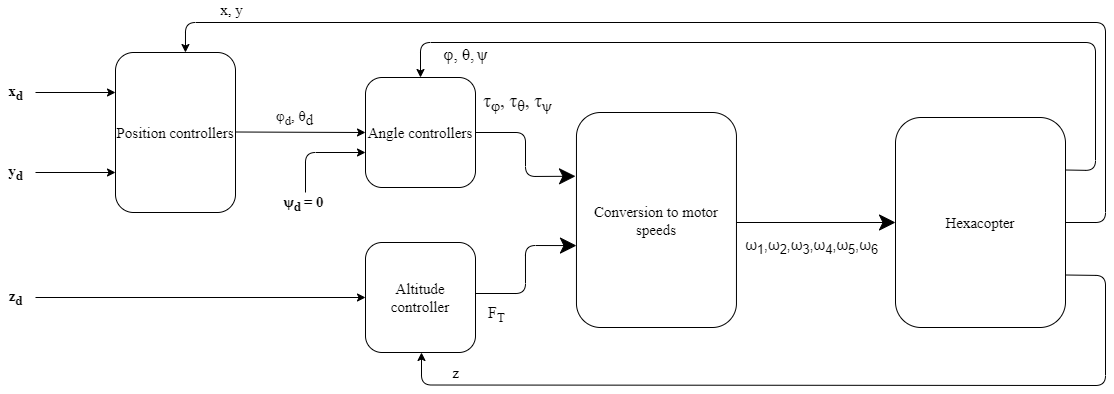
\includegraphics[width=\columnwidth]{PID_Hexacopter.PNG}%
	\caption{Complete PID control system block diagram}%
	\label{fig:PID_Hexacopter}%
\end{figure}

The gains of each controller were tuned independently using the Simulink Design Optimization Package. The Response Optimizer app within this package uses gradient descent to tune the controller gains in order to achieve the specified performance of step response. The gains achieved using this method are given in Table \ref{table:PID_Gains}.
\begin{table}[htb]\label{table:PID_Gains}
\begin{center}
\begin{tabular}{||c|c|c||} 
 \hline
 Controller & Gain & Value\\ [0.5ex] 
 \hline\hline
 \multirow{2}{7em}{Roll Angle}& K\textsubscript{P,$\phi$} & 2.688 \\ 
 \cline{2-3}
  &K\textsubscript{D,$\phi$} & 2.385 \\
 \hline
  \multirow{2}{7em}{Pitch Angle}& K\textsubscript{P,$\theta$} & 2.688 \\
 \cline{2-3}
  &K\textsubscript{D,$\theta$} & 2.385 \\
 \hline
 \multirow{2}{7em}{Yaw Angle}& K\textsubscript{P,$\psi$} & 0.759 \\
 \cline{2-3}
 &K\textsubscript{D,$\psi$} & 0.664 \\
 \hline
 \multirow{2}{7em}{x Position}& K\textsubscript{P,$x$} & 3.322 \\
 \cline{2-3}
 &K\textsubscript{D,$x$} & 2.020 \\
 \hline
 \multirow{2}{7em}{y Position}& K\textsubscript{P,$y$} & 1.471 \\
 \cline{2-3}
 &K\textsubscript{D,$y$} & 1.681 \\
 \hline
 \multirow{2}{7em}{z Position}& K\textsubscript{P,$z$} & 218.4 \\
 \cline{2-3}
 &K\textsubscript{D,$z$} & 162.5 \\
 \hline
\end{tabular}
\caption{PD controller gains}
\end{center}
\end{table}

\FloatBarrier

\subsection{Preliminary Results}
The PD control system was implemented in Simulink and its ability to stabilise the Euler angles from significant initial conditions was tested. The system simultaneously stabilises the position and counteracts any deviations from the origin, as seen in \figref{fig:PID_Stabilise}.
\begin{figure}[htb]
\begin{center}
	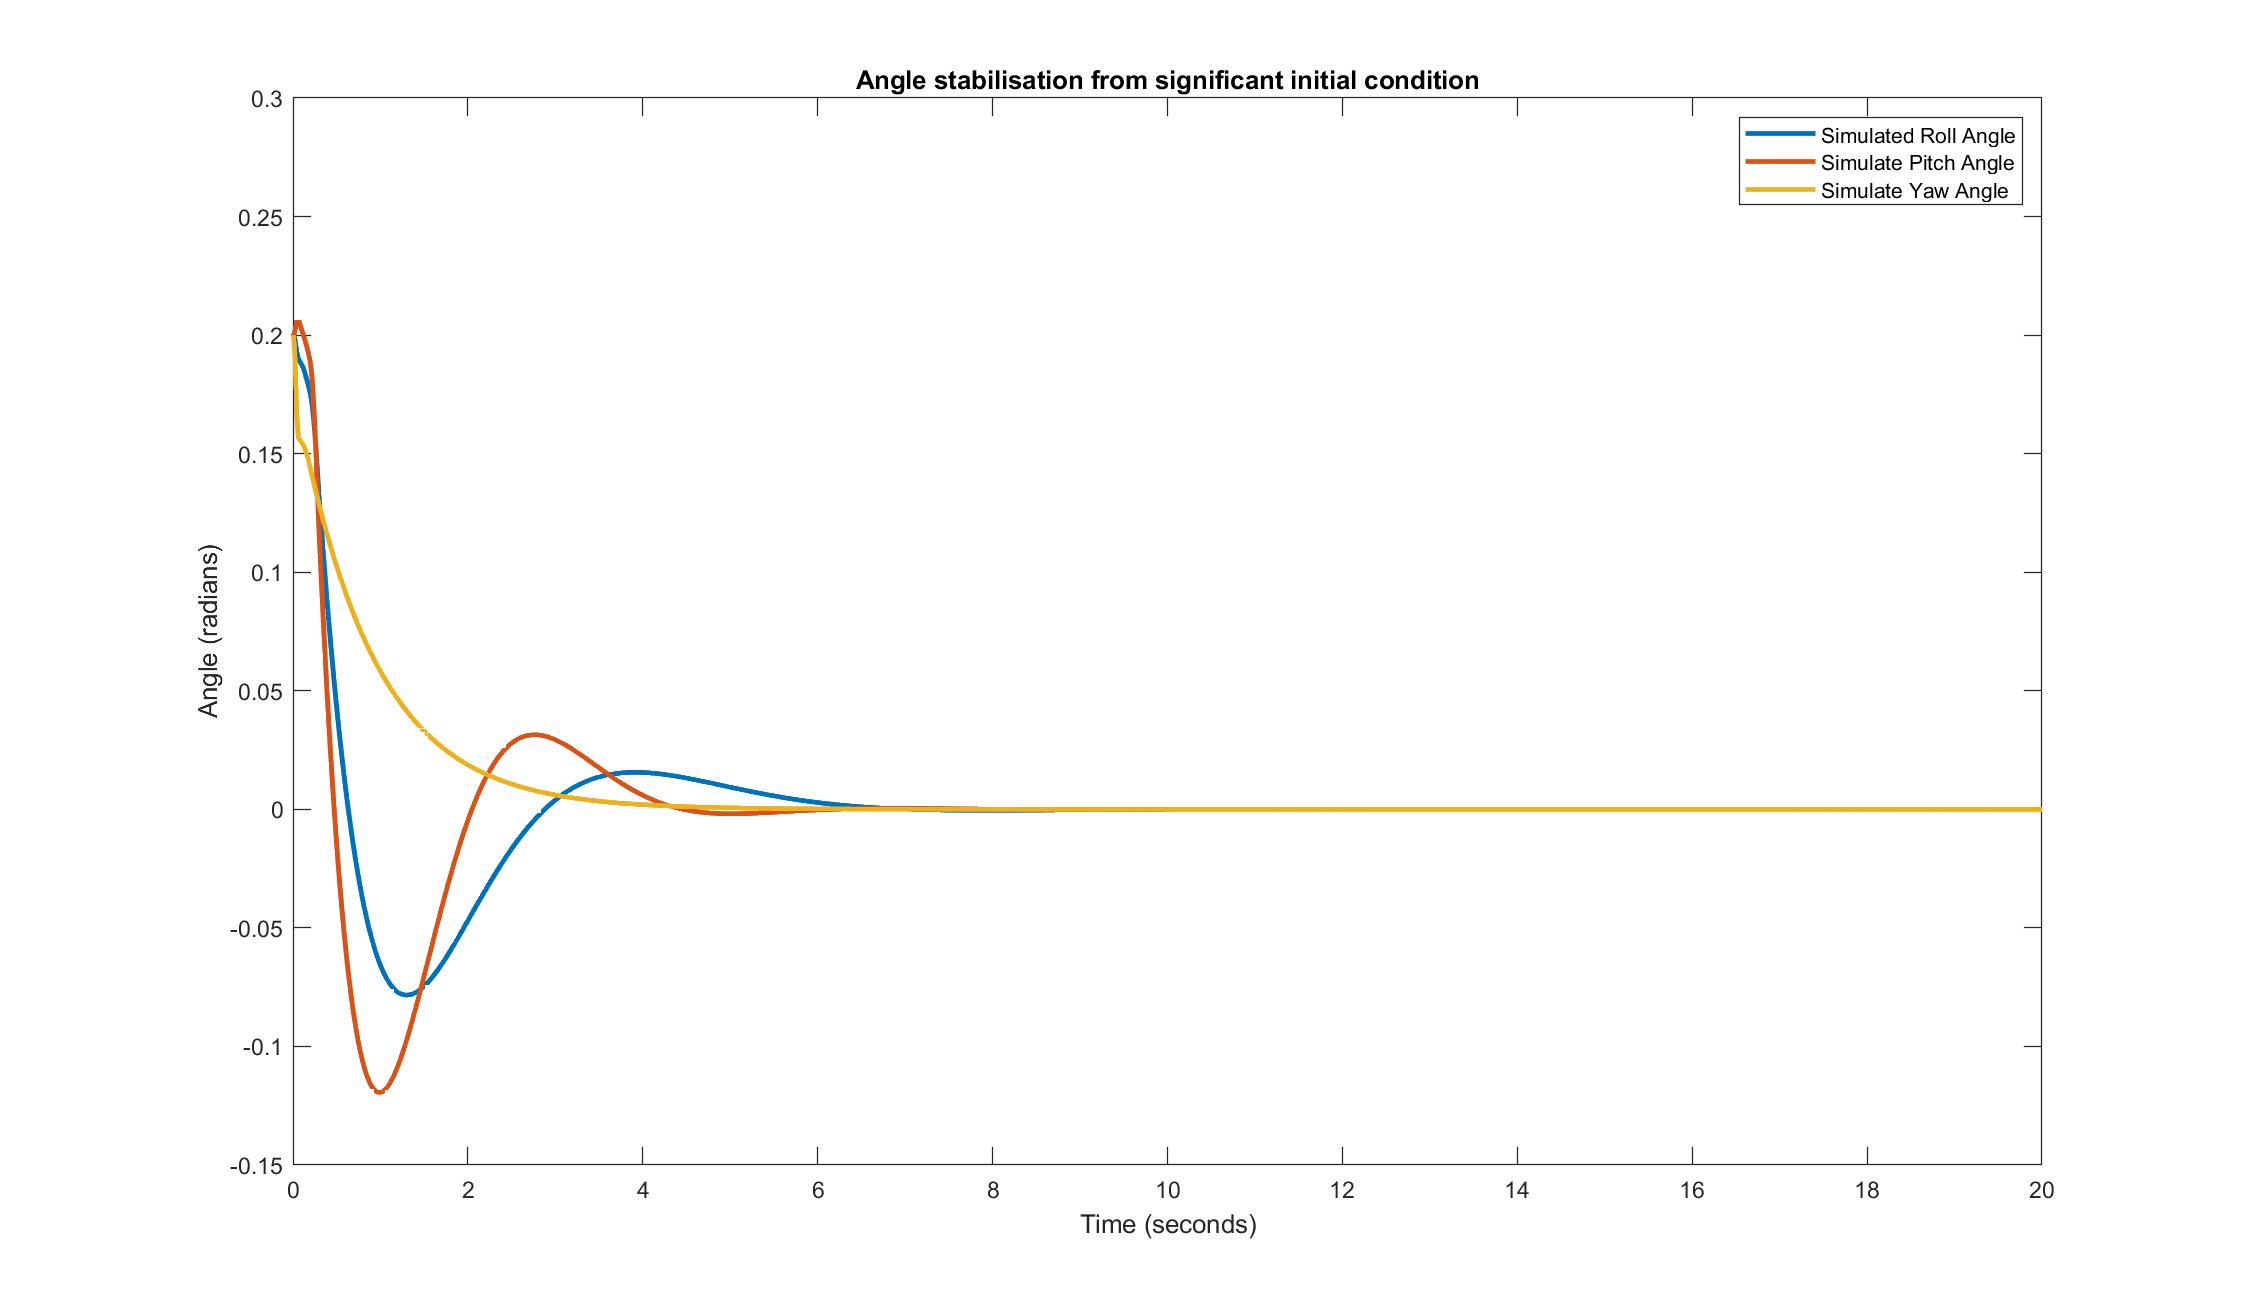
\includegraphics[width=70mm]{/PID_Results/Stabilise_Angles}
	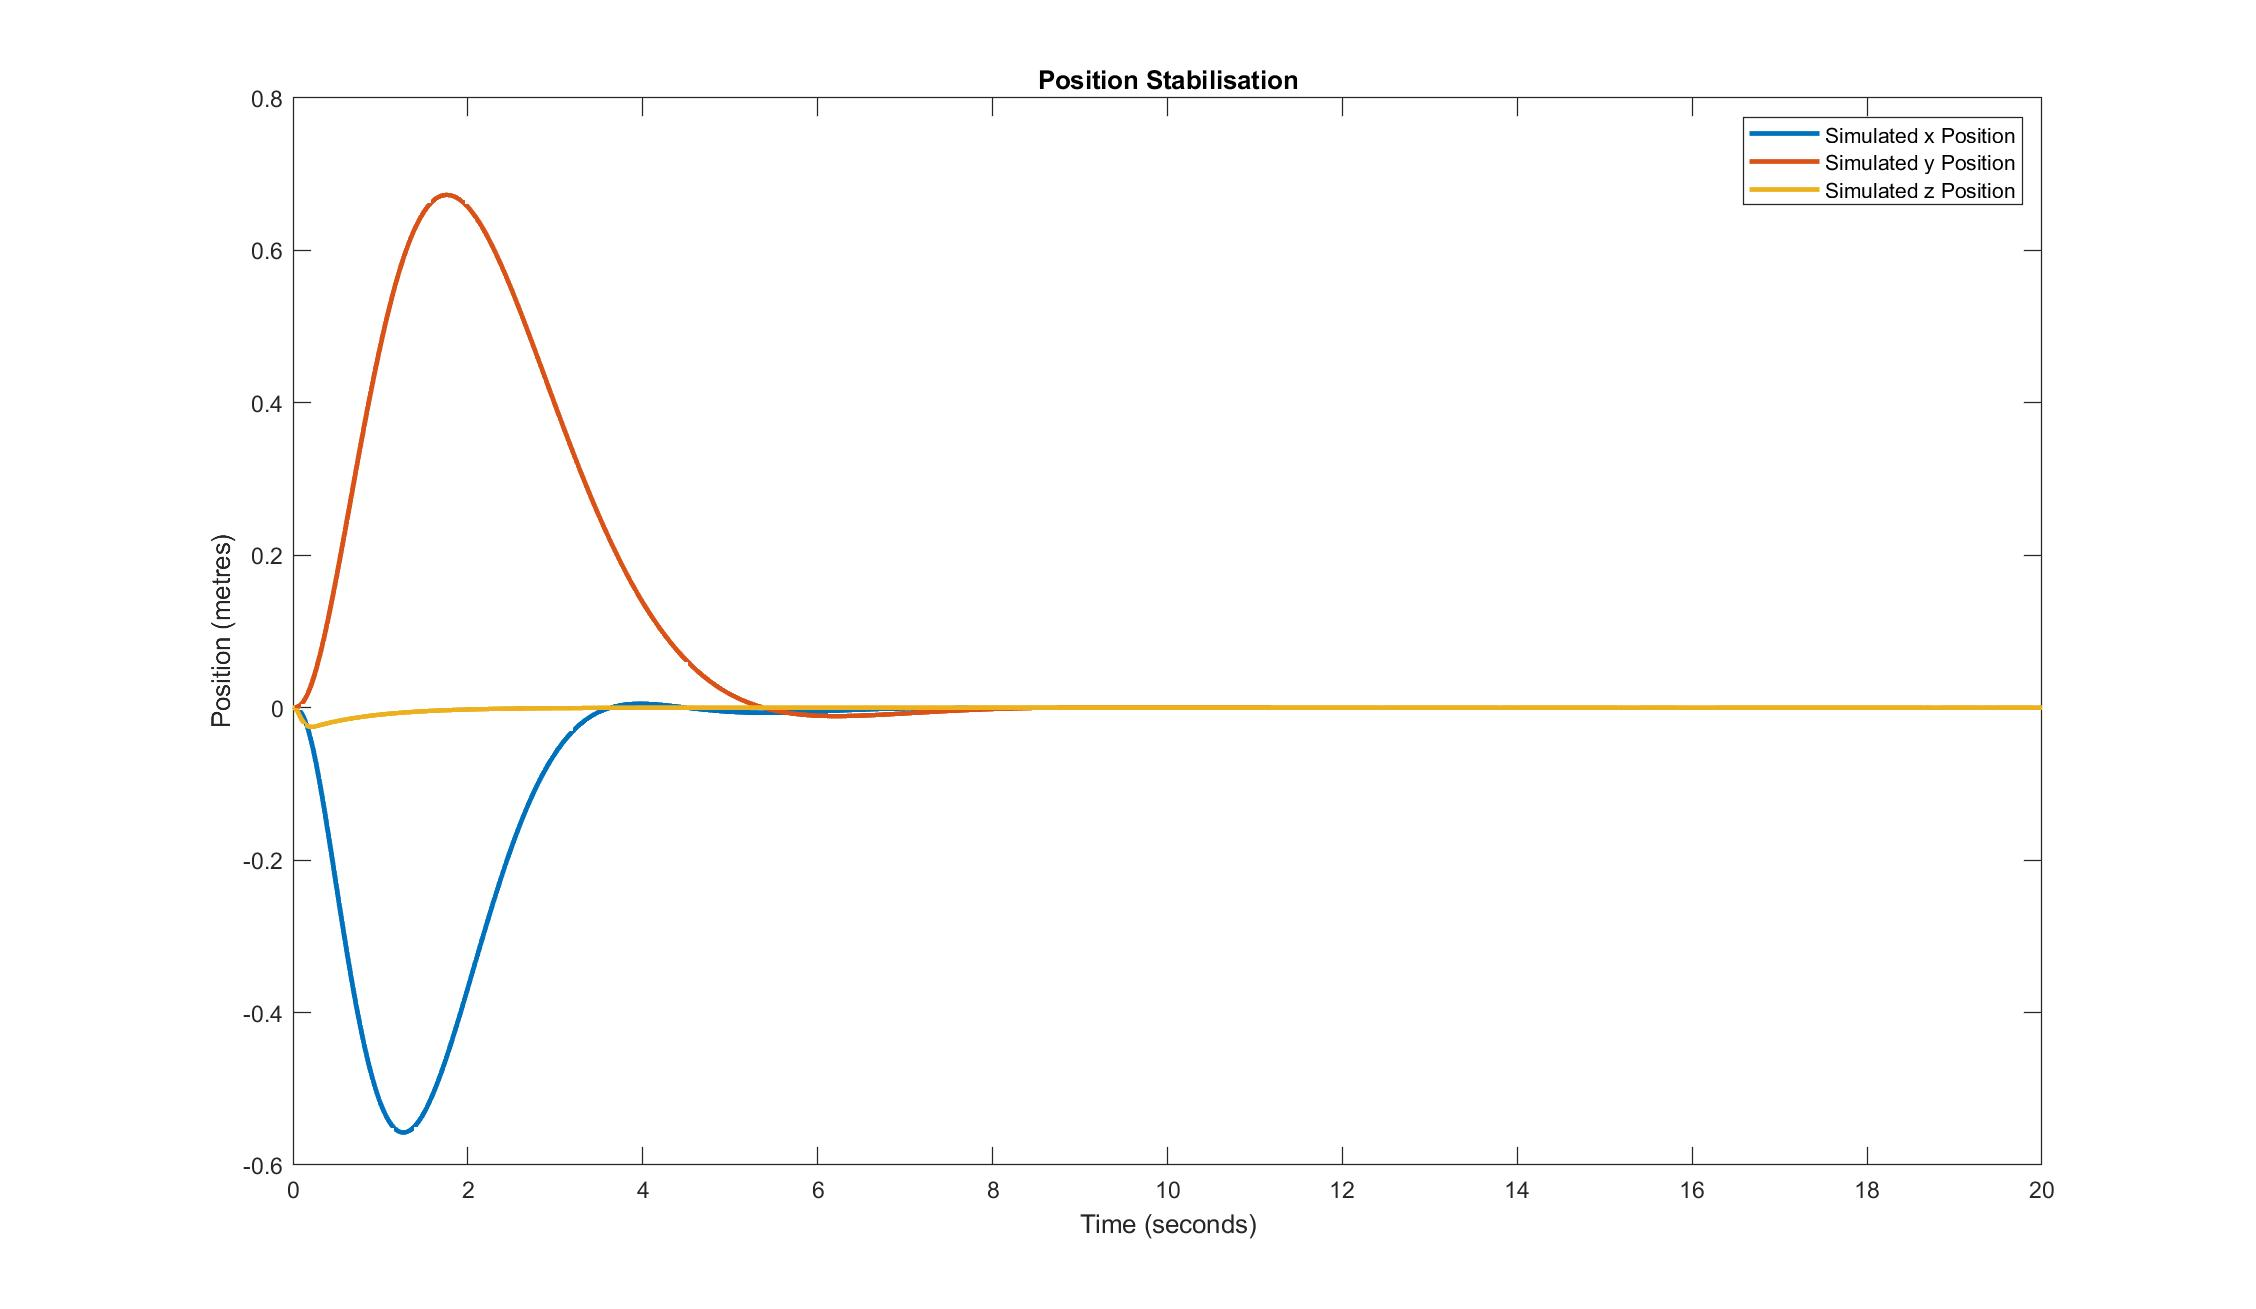
\includegraphics[width=70mm]{/PID_Results/Stabilise_Position}%
	\end{center}
	\caption{PD system stabilisation from significant initial angles}%
	\label{fig:PID_Stabilise}%
\end{figure}

The system tracking capabilities were also tested with step reference inputs. The step responses for roll angle, x position and altitude can be seen in \figref{fig:PID_Results}. The step response of the other angles ($\theta$, $\psi$) are very similar to the roll angle response and the y position response is similar to that of the x position, therefore these responses are not shown for brevity.
\begin{figure}[htb]
\begin{center}
	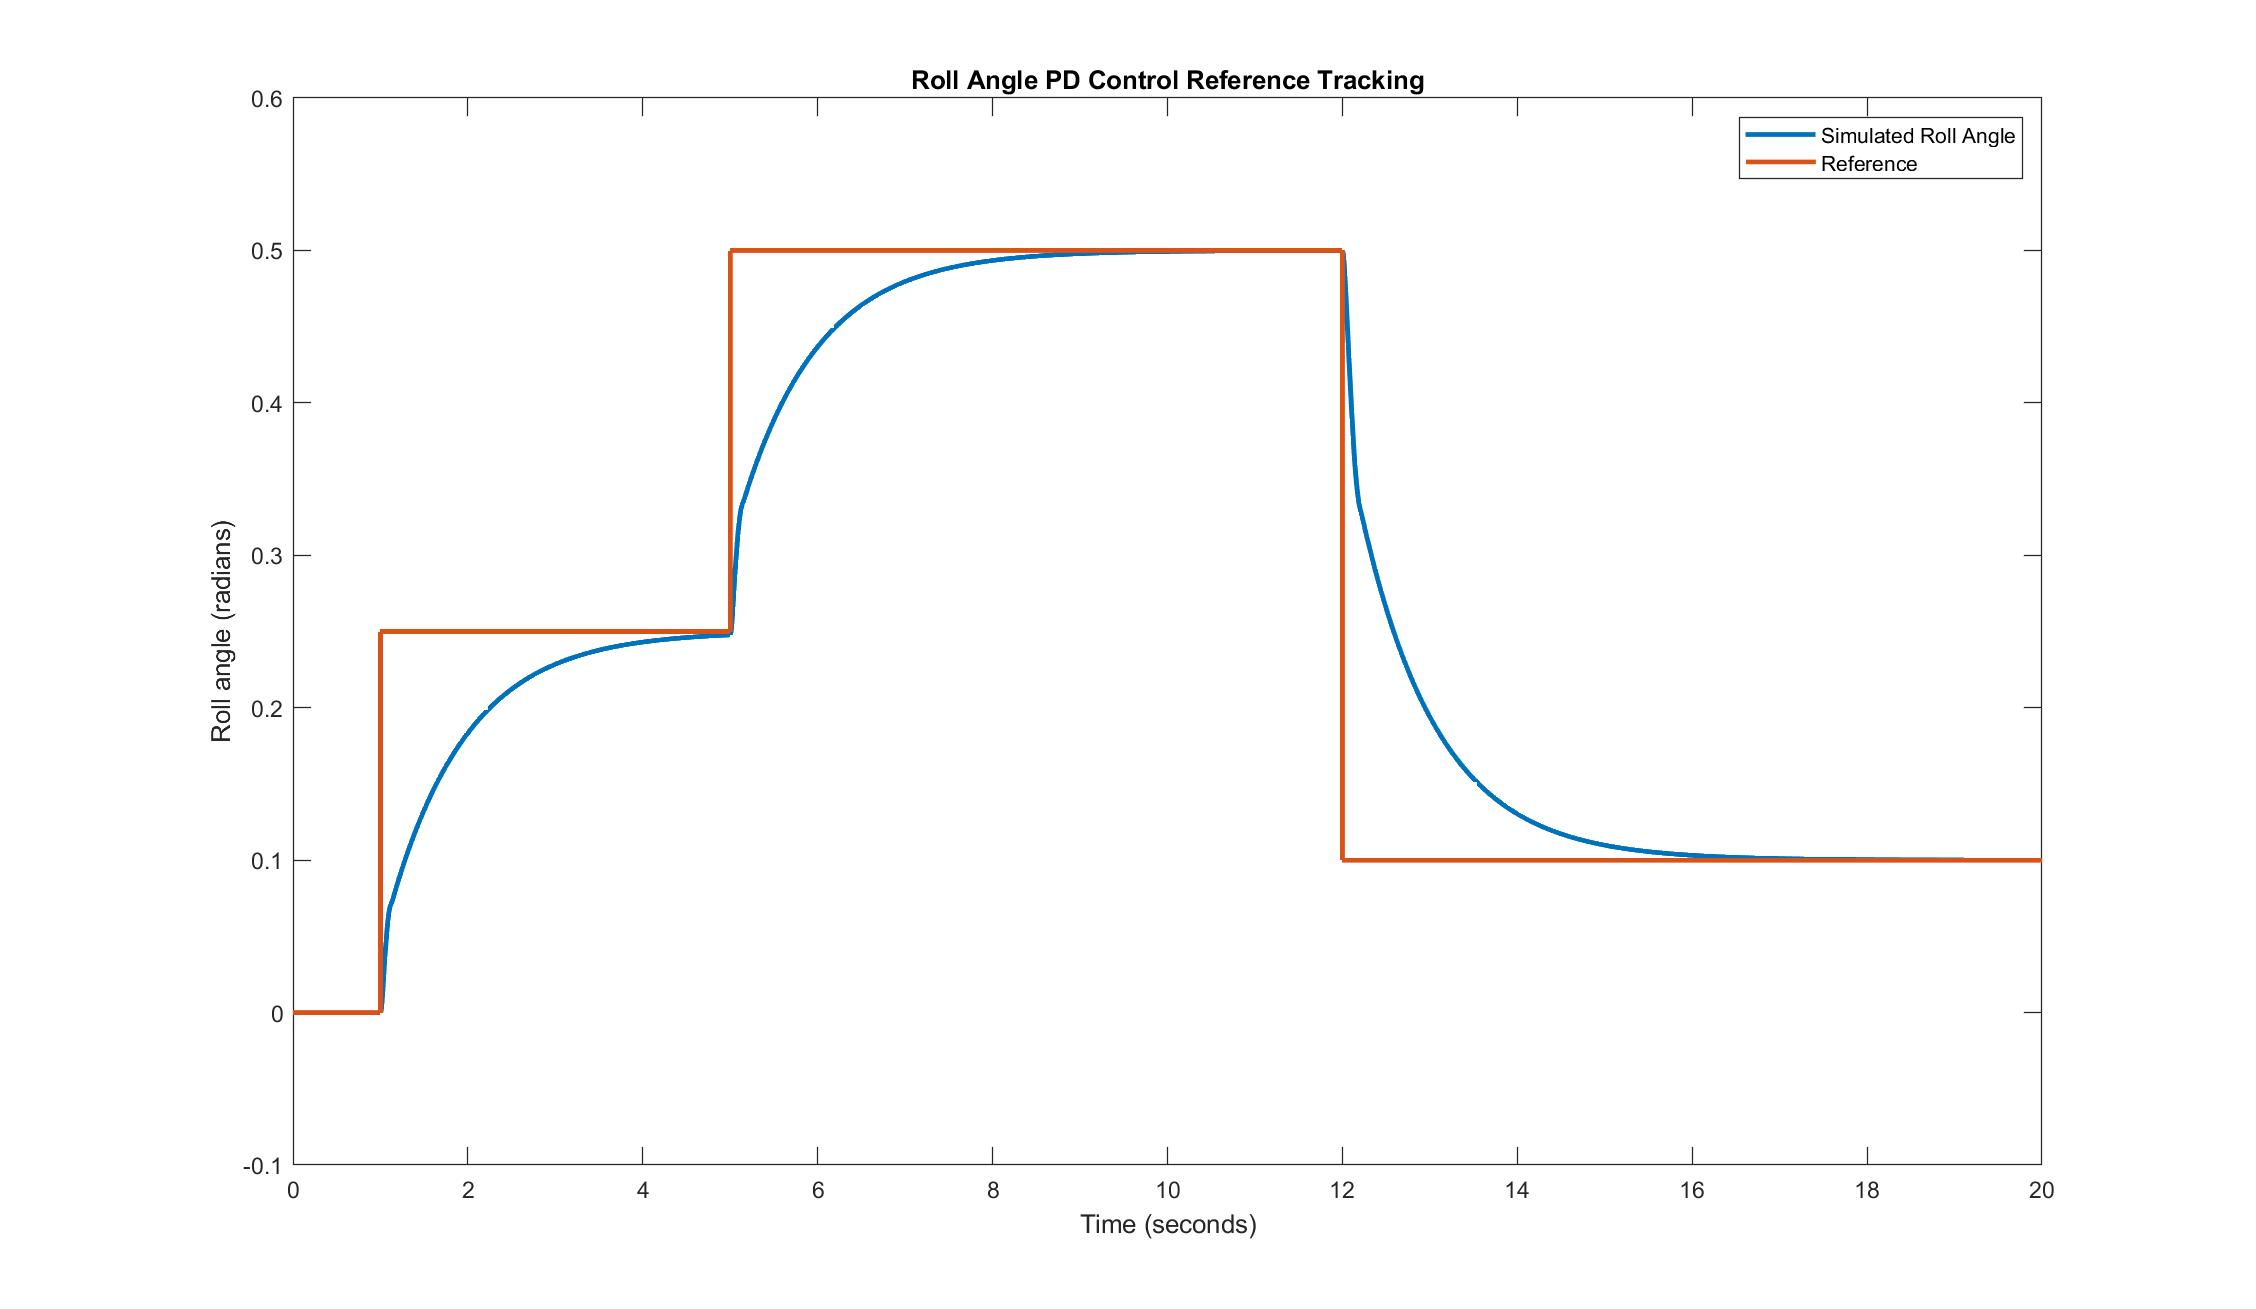
\includegraphics[width=75mm]{/PID_Results/PhiTracking_Steps2}\\
	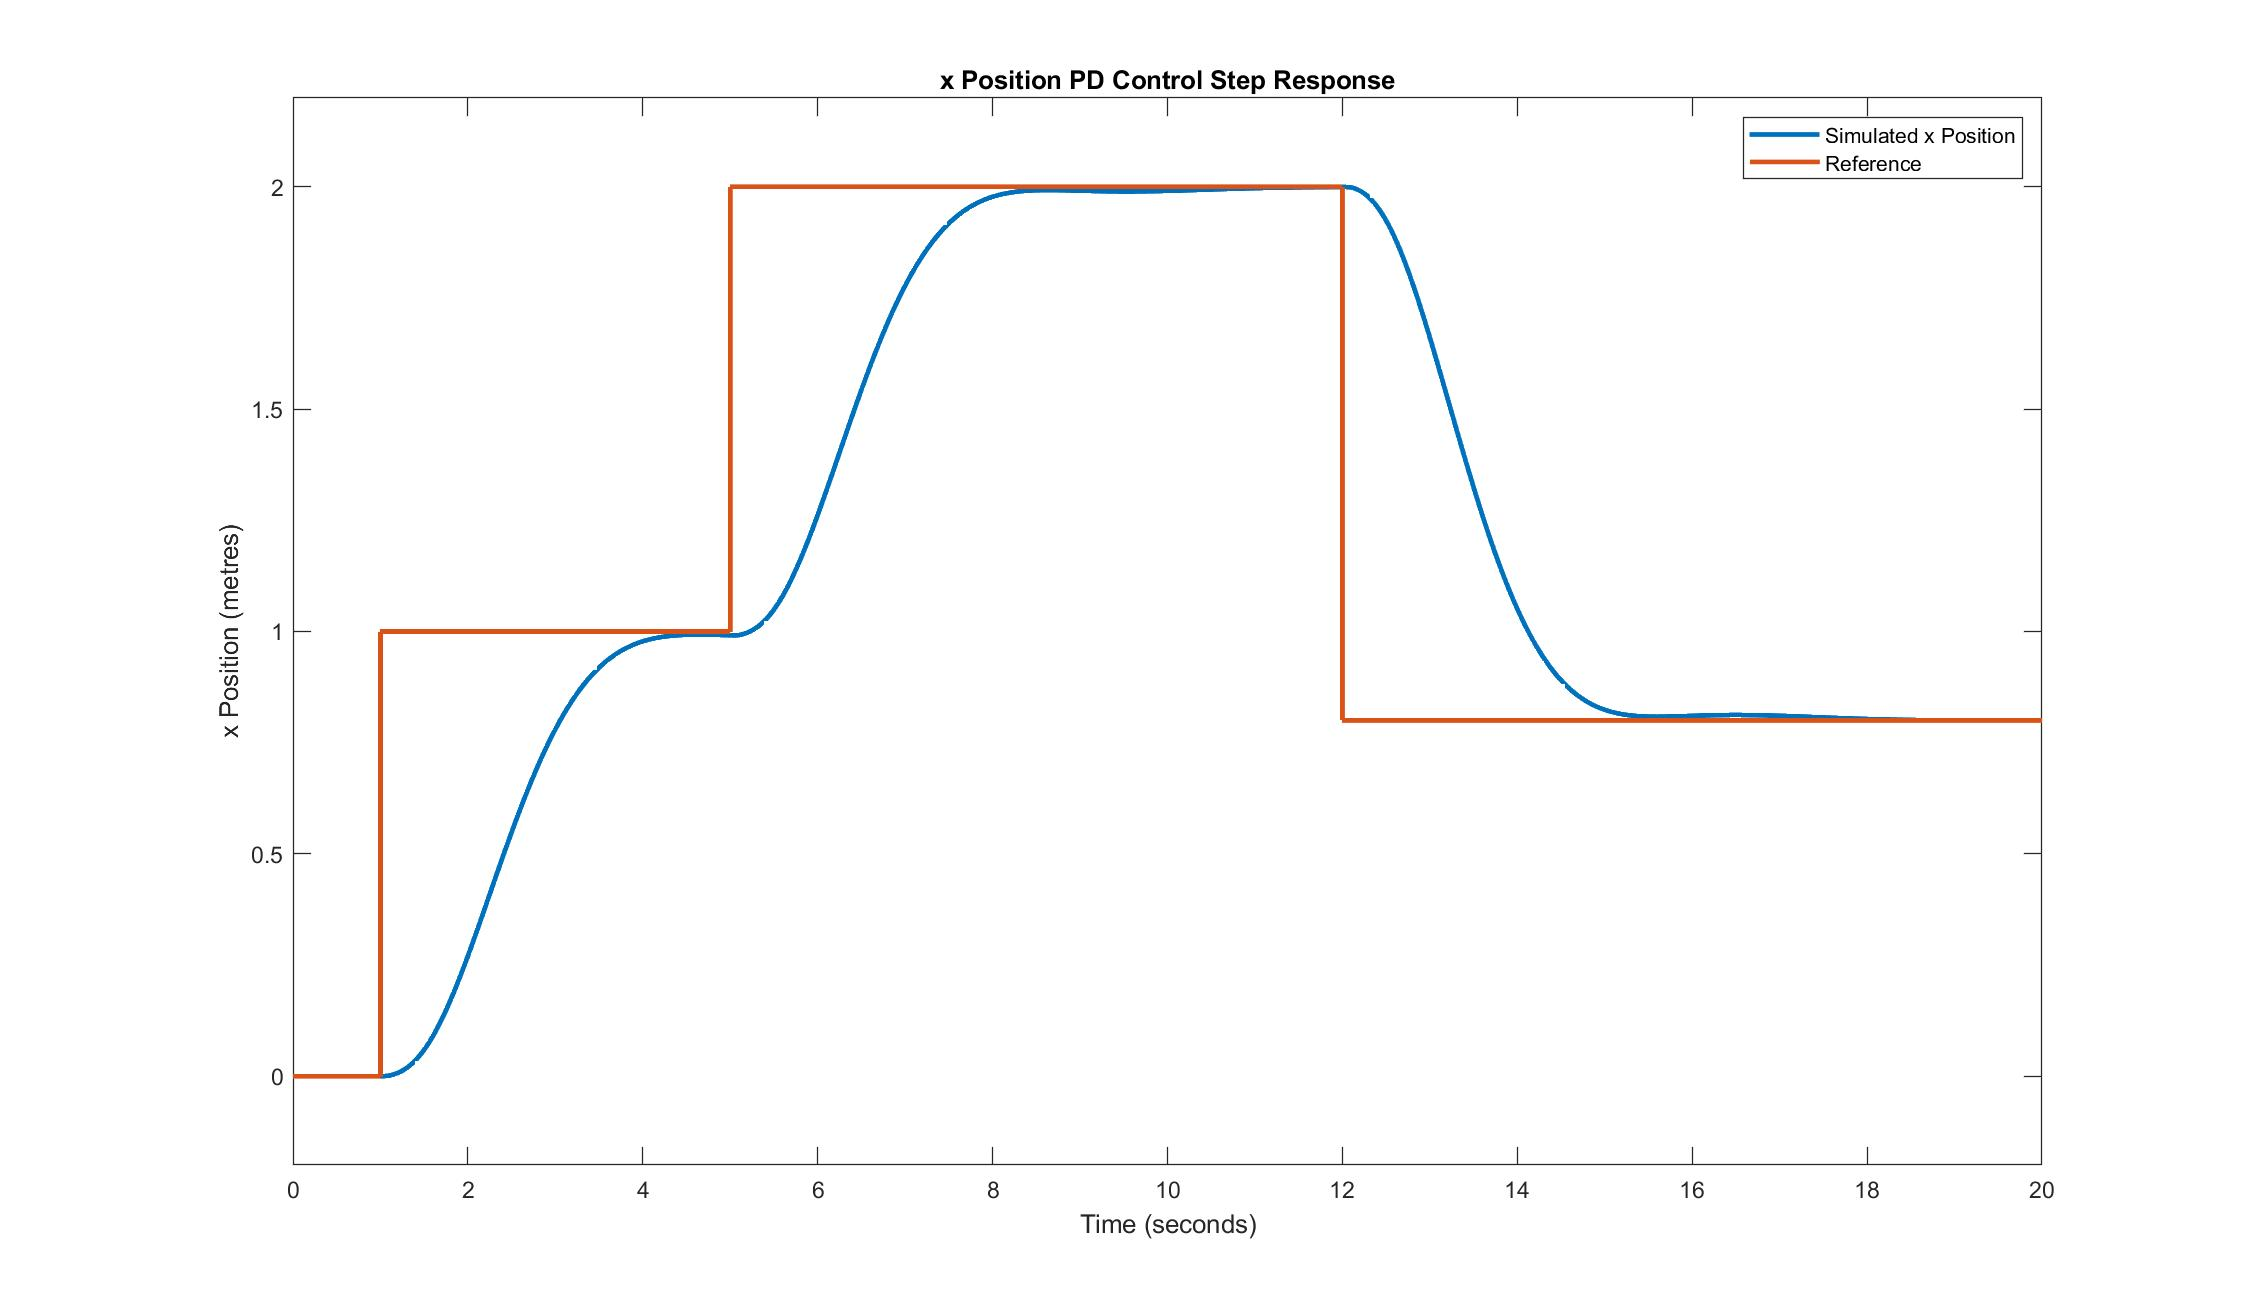
\includegraphics[width=75mm]{/PID_Results/xTracking_Steps2}%
	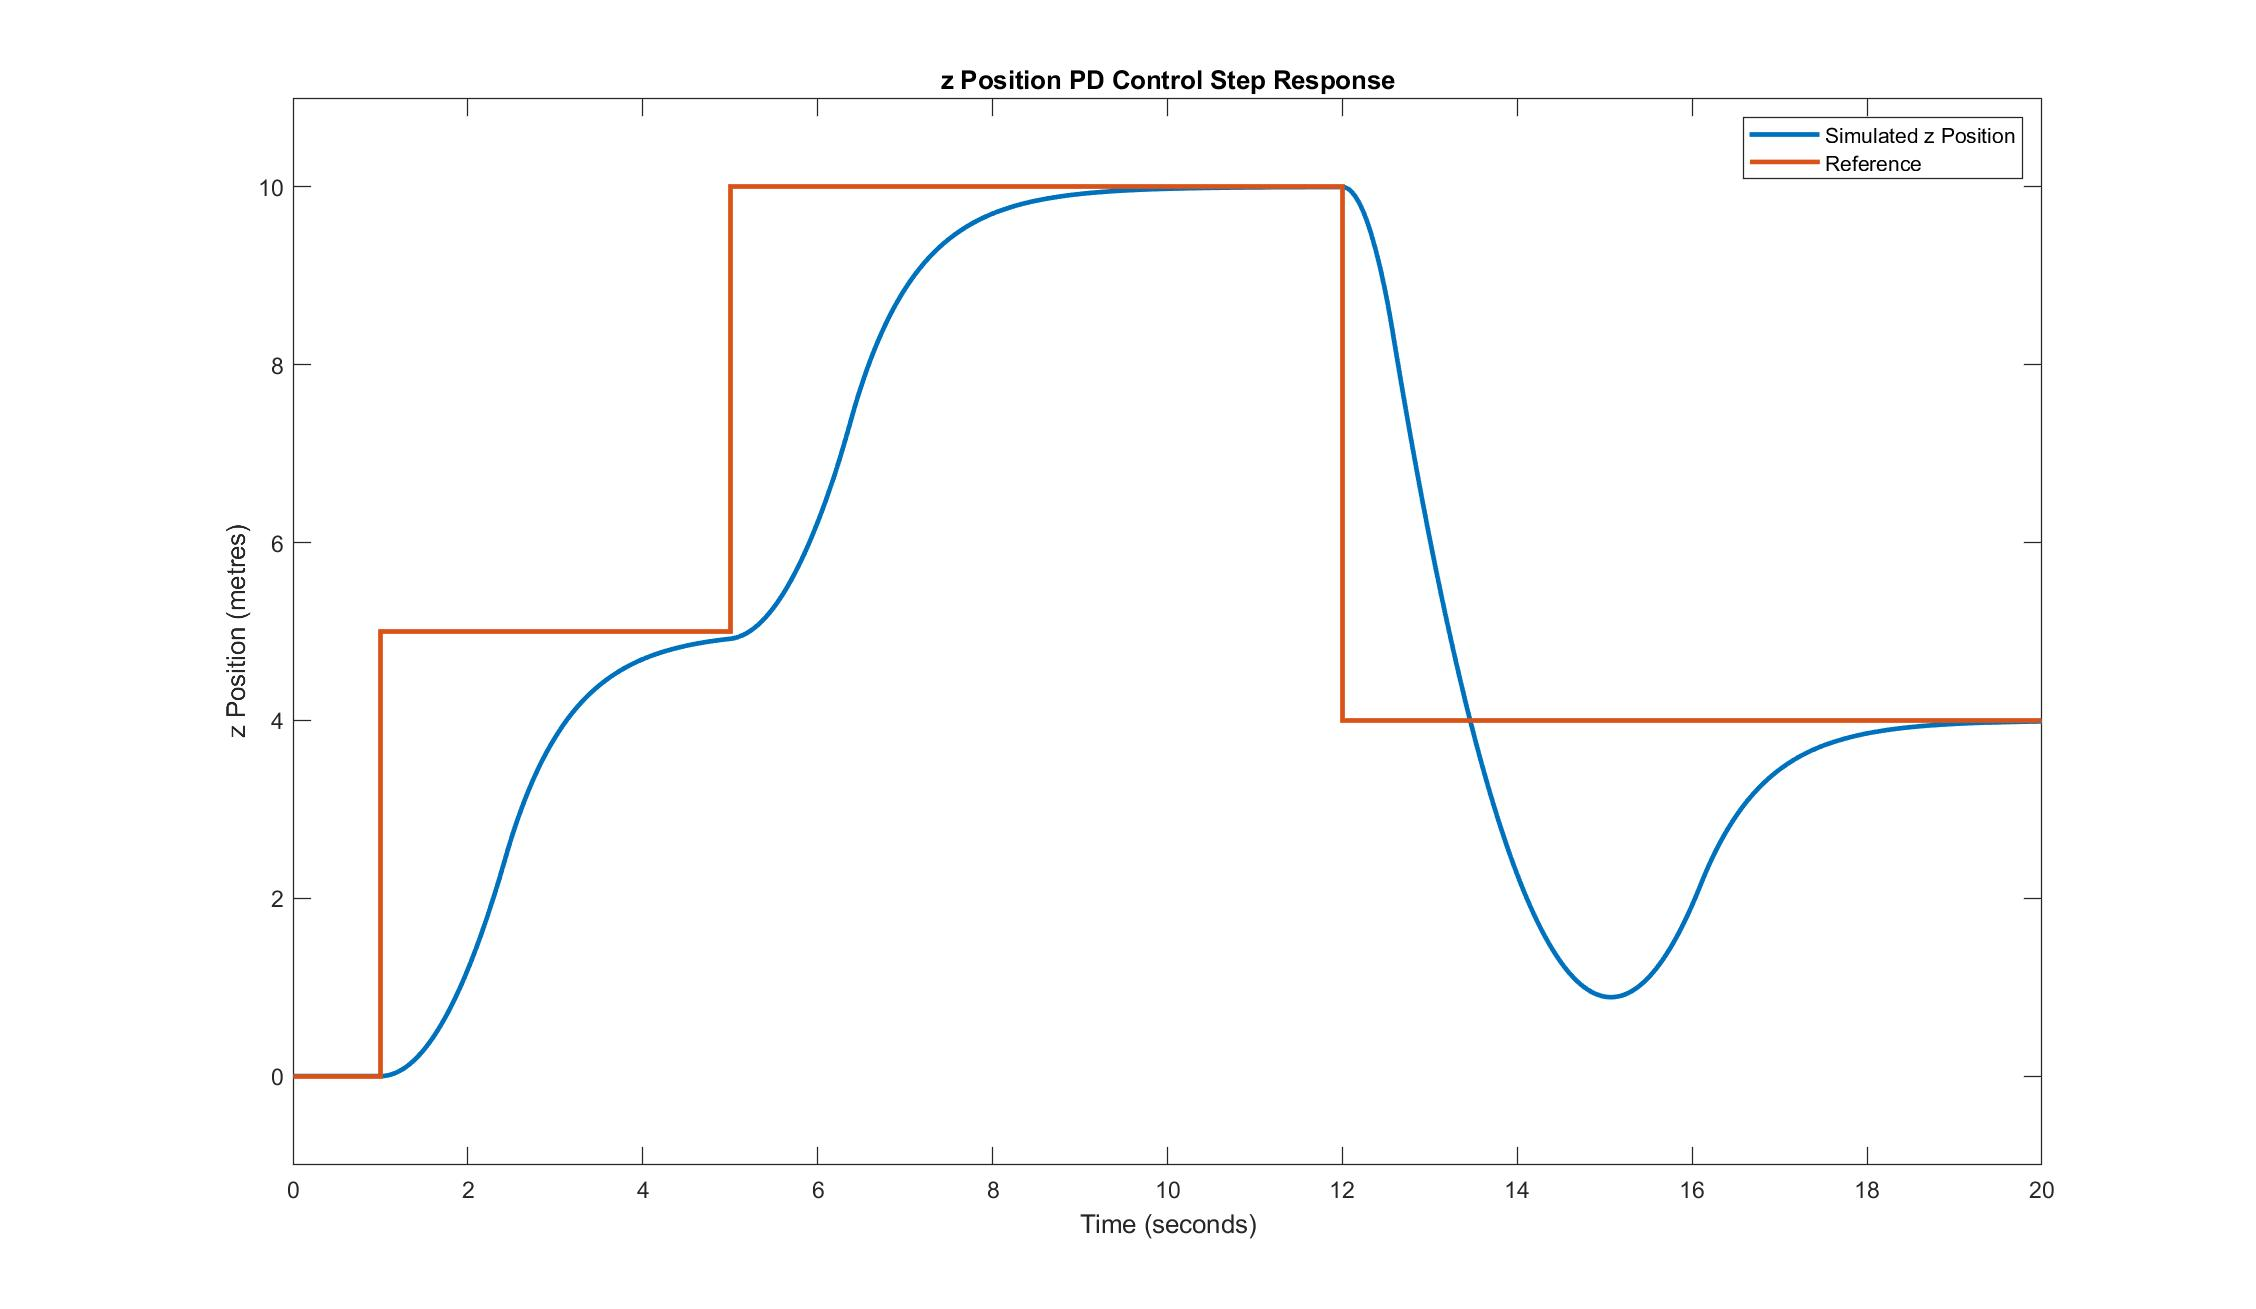
\includegraphics[width=75mm]{/PID_Results/zTracking_Steps2}%
	\end{center}
	\caption{PD system step responses}%
	\label{fig:PID_Results}%
\end{figure}
The control system was also shown to be reasonably effective in tracking a sinusoidal position command, as shown in \figref{fig:PID_Sine}.
\begin{figure}[htb]
\begin{center}
	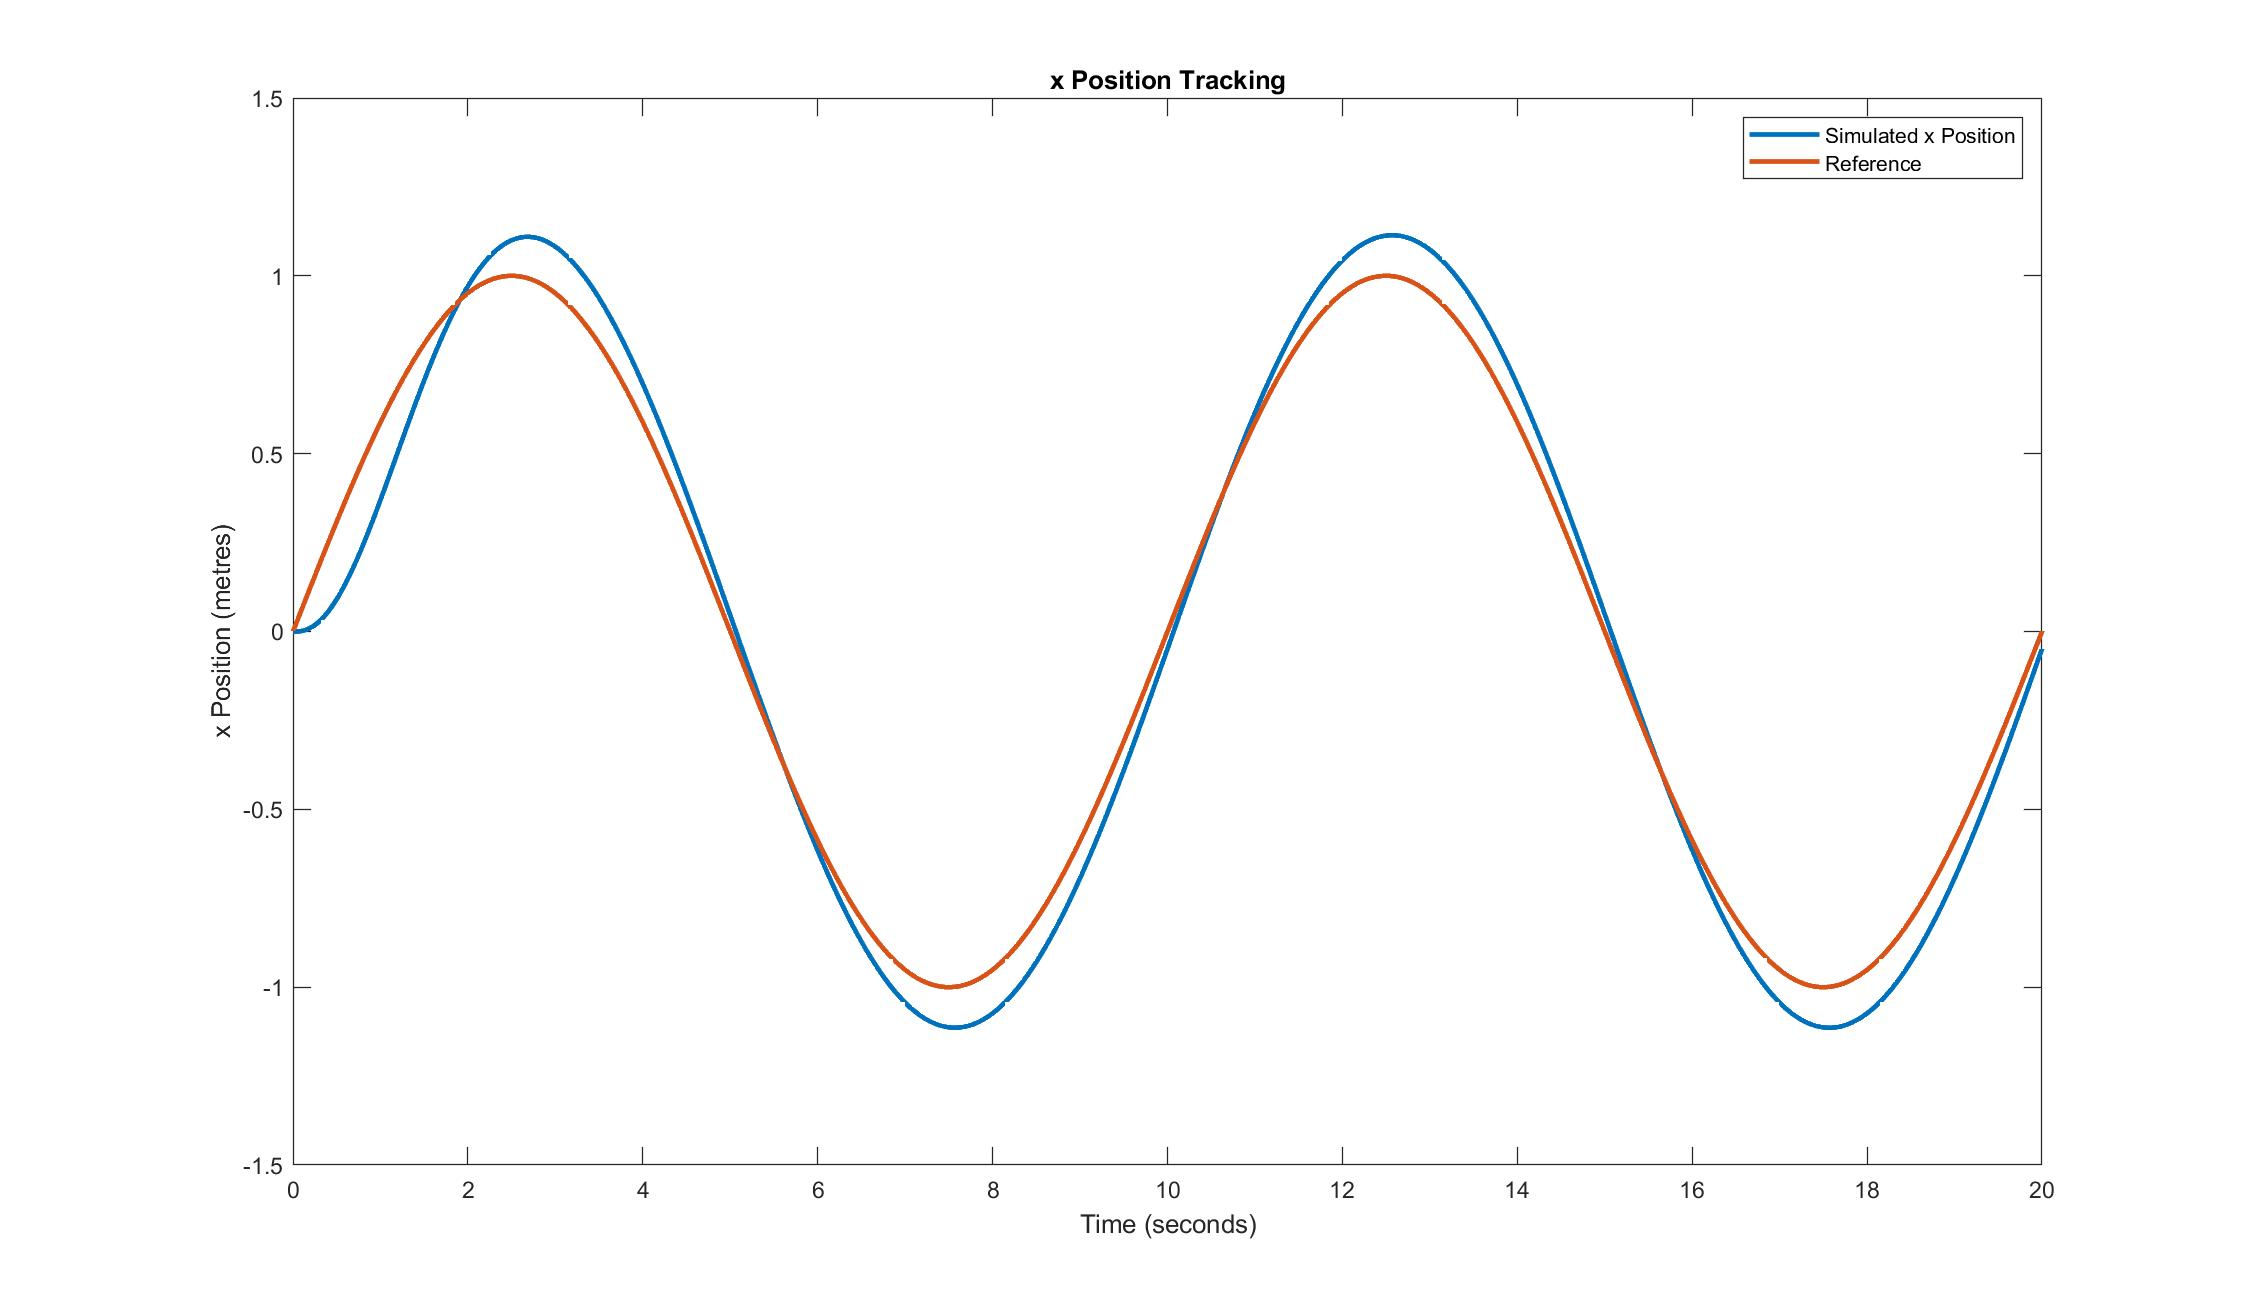
\includegraphics[width=80mm]{/PID_Results/xTracking_Sine2.jpg}%
	\end{center}
	\caption{PID Position tracking}%
	\label{fig:PID_Sine}%
\end{figure}

The results show that this system is effective in stabilising the aircraft around a hovering point in the absence of major disturbances. It is also able to respond to relatively small positional step commands. However, this control method is limited since it neglects the nonlinearities of the physical system. For example, it is ineffective with a non-zero yaw angle due to approximations made in the simplification of the model. The system is also prone to saturation when subject to large step commands.

\FloatBarrier
\section{Backstepping Control}
In order to improve upon the performance of the previous controller, the recursive Lyapunov-based control method known as backstepping will be applied to the multi-rotor system. The mathematical background of this method is discussed in Section \ref{section:BacksteppingBackground}.
\subsection{Simplified State Space Model}
The states used by the backstepping controller will be each of the positions in the Earth frame as well as their respective velocities. In order to simplify notation, the states will be referred to as $x_{i}$ and are defined as:
\begin{equation}\label{eqn:stateDef}
x=
\begin{bmatrix}
x_{1}\\
x_{2}\\
x_{3}\\
x_{4}\\
x_{5}\\
x_{6}\\
x_{7}\\
x_{8}\\
x_{9}\\
x_{10}\\
x_{11}\\
x_{12}
\end{bmatrix}
=
\begin{bmatrix}
\phi\\
\dot{\phi}\\
\theta\\
\dot{\theta}\\
\psi\\
\dot{\psi}\\
x\\
\dot{x}\\
y\\
\dot{y}\\
z\\
\dot{z}
\end{bmatrix}
\end{equation}

As seen in Section \ref{{section:SimpleModel}}, the state space model which was presented in Section \ref{section:ModelDynamics}, is able to be greatly simplified by making a number of assumptions. For the purposes of this controller, the small angle approximation will be used in order to simplify the relationship between the torques and the Euler angles. That is, the relationship in Equation \ref{eqn:simpleState1} will be assumed true. Applying this to Equation \ref{eqn:state3} gives the following:

\begin{equation}
\begin{bmatrix}
\dot{x}_{2}\\
\dot{x}_{4}\\
\dot{x}_{6}
\end{bmatrix}
=
\begin{bmatrix}
a_{1}x_{4}x_{6}+b_{1}\tau_{\phi}\\
a_{2}x_{2}x_{6}+b_{2}\tau_{\theta}\\
a_{3}x_{2}x_{4}+b_{3}\tau_{\psi}
\end{bmatrix}
\end{equation}
with $a_{1}=\frac{I_{yy}-I_{zz}}{I_{xx}}$, $a_{2}=\frac{I_{zz}-I_{xx}}{I_{yy}}$, $a_{3}=\frac{I_{xx}-I_{yy}}{I_{zz}}$, $b_{1}=\frac{1}{I_{xx}}$, $b_{2}=\frac{1}{I_{yy}}$, $b_{3}=\frac{1}{I_{zz}}$. Now, the simplified state space model may be expressed:

\begin{equation}\label{eqn:simpleStateModel}
\begin{bmatrix}
\dot{x}_{1}\\
\dot{x}_{2}\\
\dot{x}_{3}\\
\dot{x}_{4}\\
\dot{x}_{5}\\
\dot{x}_{6}\\
\dot{x}_{7}\\
\dot{x}_{8}\\
\dot{x}_{9}\\
\dot{x}_{10}\\
\dot{x}_{11}\\
\dot{x}_{12}
\end{bmatrix}
=
\begin{bmatrix}
x_{2}\\
a_{1}x_{4}x_{6}+b_{1}\tau_{\phi}\\
x_{4}\\
a_{2}x_{2}x_{4}+b_{2}\tau_{\theta}\\
x_{6}\\
a_{3}x_{2}x_{4}+b_{3}\tau_{\psi}\\
x_{8}\\
[cos(x_{1})sin(x_{3})cos(x_{5})+sin(x_{1})sin(x_{5})]\frac{F_{T}}{m}\\
x_{10}\\
[cos(x_{1})sin(x_{3})sin(x_{5})-sin(x_{1})cos(x_{5})]\frac{F_{T}}{m}\\
x_{12}\\
[cos(x_{1})cos(x_{3})]\frac{F_{T}}{m}-g
\end{bmatrix}
\end{equation}

\subsection{Attitude Control}
Consider the tracking error of the roll angle, i.e. the first state:
\[z_{1}= x_{1d}-x_{1}\]

Choose a candidate Lyapunov function such that it is positive definite:
\[V(z_{1})=\frac{1}{2}z_{1}^{2}\]
Taking its derivative gives:

\[\dot{V}(z_{1})=z_{1}\dot{z}_{1}\]

A control Lyapunov function must have a negative definite derivative, therefore \(\dot{z_{1}}\) is chosen to be \(-K_{1}z_{1}\) with constant gain \(K_{1}>0\). This gives the following result:
\[\dot{V}(z_{1})=-K_{1}z_{1}^{2}\]
Now, take the derivative of \(z_{1}\) and substitute our chosen value.
\begin{equation*}
\begin{split}
\dot{z_{1}}&=\dot{x}_{1d}-\dot{x}_{1}\\
-K_{1}z_{1}&=\dot{x}_{1d}-x_{2}\\
\end{split}
\end{equation*}
Now, choose a virtual control \(x_{2d}\) to satisfy this relationship:
\[x_{2d}=\dot{x}_{1d}+K_{1}z_{1}\]
Now consider the tracking error of the second state:
\begin{equation*}
\begin{split}
z_{2}&=x_{2d}-x_{2}\\
&=\dot{x}_{1d}+K_{1}z_{1}-x_{2}
\end{split}
\end{equation*}
Now choose a second candidate Lyapunov function:
\[V(z_{1},z_{2})=\frac{1}{2}(z_{1}^2+z_{2}^2)\]
Then take its derivative:
\begin{equation*}
\begin{split}
\dot{V}(z_{1},z_{2})&=\dot{V}(z_{1})+z_{2}\dot{z}_{2}\\
&=-K_{1}z_{1}^{2}+z_{2}\dot{z}_{2}
\end{split}
\end{equation*}
Now to ensure \(\dot{V}(z_{1},z_{2})\) is negative definite, choose \(\dot{z}_{2}=-K_{2}z_{2}\) with constant \(K_{2}>0\). This gives the following result:
\begin{equation*}
\begin{split}
\dot{z}_{2}&=\ddot{x}_{1d}+K_{1}\dot{z}_{1}-\dot{x}_{2}\\
-K_{2}z_{2}&=\ddot{x}_{1d}+K_{1}(\dot{x}_{1d}-x_{2})-a_{1}x_{4}x_{6}-b_{1}\tau_{\phi}
\end{split}
\end{equation*}
Using this result, it is possible to choose a control value for the input \(\tau_{\phi}\) which will stabilise the roll angle:
\begin{equation*}
\tau_{\phi}=\frac{1}{b_{1}}(\ddot{x}_{1d}+K_{1}(\dot{x}_{1d}-x_{2})-a_{1}x_{4}x_{6}+K_{2}z_{2})
\end{equation*}
The same steps can be followed to stabilise both the pitch and yaw angles with control inputs \(\tau_{\theta}\) and \(\tau_{\psi}\) respectively. These control laws are given in \eqref{eqn:BackstepAngleLaws}.

\begin{equation}\label{eqn:BackstepAngleLaws}
\begin{split}
\tau_{\theta}&=\frac{1}{b_{2}}\left(\ddot{x}_{3d}+K_{3}(\dot{x}_{3d}-x_{4})-a_{2}x_{2}x_{6}+K_{4}z_{4}\right)\\
\tau_{\psi}&=\frac{1}{b_{3}}\left(\ddot{x}_{5d}+K_{5}(\dot{x}_{5d}-x_{6})-a_{3}x_{2}x_{4}+K_{6}z_{6}\right)
\end{split}
\end{equation}

angle results, stabilisation...

\subsection{Position Control}
The control laws developed in the previous section successfully allow stabilisation and tracking of the vehicle's attitude, however, the objective of this control system is to allow the vehicle to track a trajectory in 3D space. First consider the tracking error of the position in the Earth frame x direction:
\[z_{7}=x_{7d}-x{7}\]
Following the same logic presented in the development of the attitude controllers, the candidate Lyapunov function is chosen as $V(z_{7})=\frac{1}{2}z_{7}^{2}$. Thus, a virtual control for $x_{8}$ is chosen to satisfy $\dot{z}_{7}=-K_{7}z_{7}$:
\[x_{8d}=\dot{x}_{7d}+K_{7}z_{7}\]

Now, consider the tracking error of the translational velocity, $z_{8}$, and its derivative:

\[
\begin{split}
z_{8}&=x_{8d}-x_{8}\\
z_{8}&=\dot{x}_{7d}+K_{7}z_{7}-x_{8}\\
\dot{z}_{8}&=\ddot{x}_{7d}+K_{7}\dot{z}_{7}-\dot{x}_{8}\\
&=\ddot{x}_{7d}+K_{7}\dot{z}_{7}-[cos(x_{1})sin(x_{3})cos(x_{5})+sin(x_{1})sin(x_{5})]\frac{F_{T}}{m}
\end{split}
\]

In order to ensure $\dot{z}_{8}=-K_{8}z_{8}$, a virtual control must be chosen. If it is assumed that the vehicle is in hovering flight and the Euler angles are stabilised around 0\textdegree, then the most logical choice of variable for a virtual control is the pitch angle ($x_{3}$). Thus, the virtual control $x_{3d}$ in Equation \ref{eqn:XPosContLaw} will be supplied as a desired value for the attitude controller developed in the previous section. 
\begin{equation}\label{eqn:XPosContLaw}
x_{3d}=sin^{-1}\left(\frac{\frac{m}{F_{T}}[K_{8}z_{8}+\ddot{x}_{7d}+K_{7}\dot{z}_{7}]-sin(x_{1})sin(x_{5})}{cos(x_{1})cos(x_{5})}\right)
\end{equation}

The y position control law, shown in \eqref{eqn:YPosContLaw}, is developed in the same way, with the roll angle ($x_{1}$) acting as the virtual control. 
\begin{equation}\label{eqn:YPosContLaw}
x_{1d}=sin^{-1}\left(\frac{-\frac{m}{F_{T}}[K_{10}z_{10}+\ddot{x}_{9d}+K_{9}\dot{z}_{9}]+cos(x_{1})sin(x_{3})sin(x_{5})}{cos(x_{5})}\right)
\end{equation}
 
The z position control law in \eqref{eqn:ZPosContLaw} is developed following the same method, with $F_{T}$ as the control input.
\begin{equation}\label{eqn:ZPosContLaw}
F_{T}=\frac{m(\ddot{x}_{11d}+K_{11}\dot{z}_{11}+K_{12}z_{12}+g)}{cos(x_{1})cos(x_{3})}
\end{equation}

\subsection{Preliminary Results}
 
The gains $K_{i}$ were tuned using the Simulink Design Optimization Package. This controller was able to stabilise the angles and positions from significant initial conditions. It was also able to travel between waypoints in 3D space. \figref{fig:Backstep_path} shows the hexacopter's path: taking off, travelling between waypoints and landing at a given location. However, this controller's response to large step inputs is unpredictable due to saturation effects. Also, note the slight steady state error in the z controller shown in \figref{fig:Backstep_posTrack}.

\begin{figure}[htb]
\begin{center}
	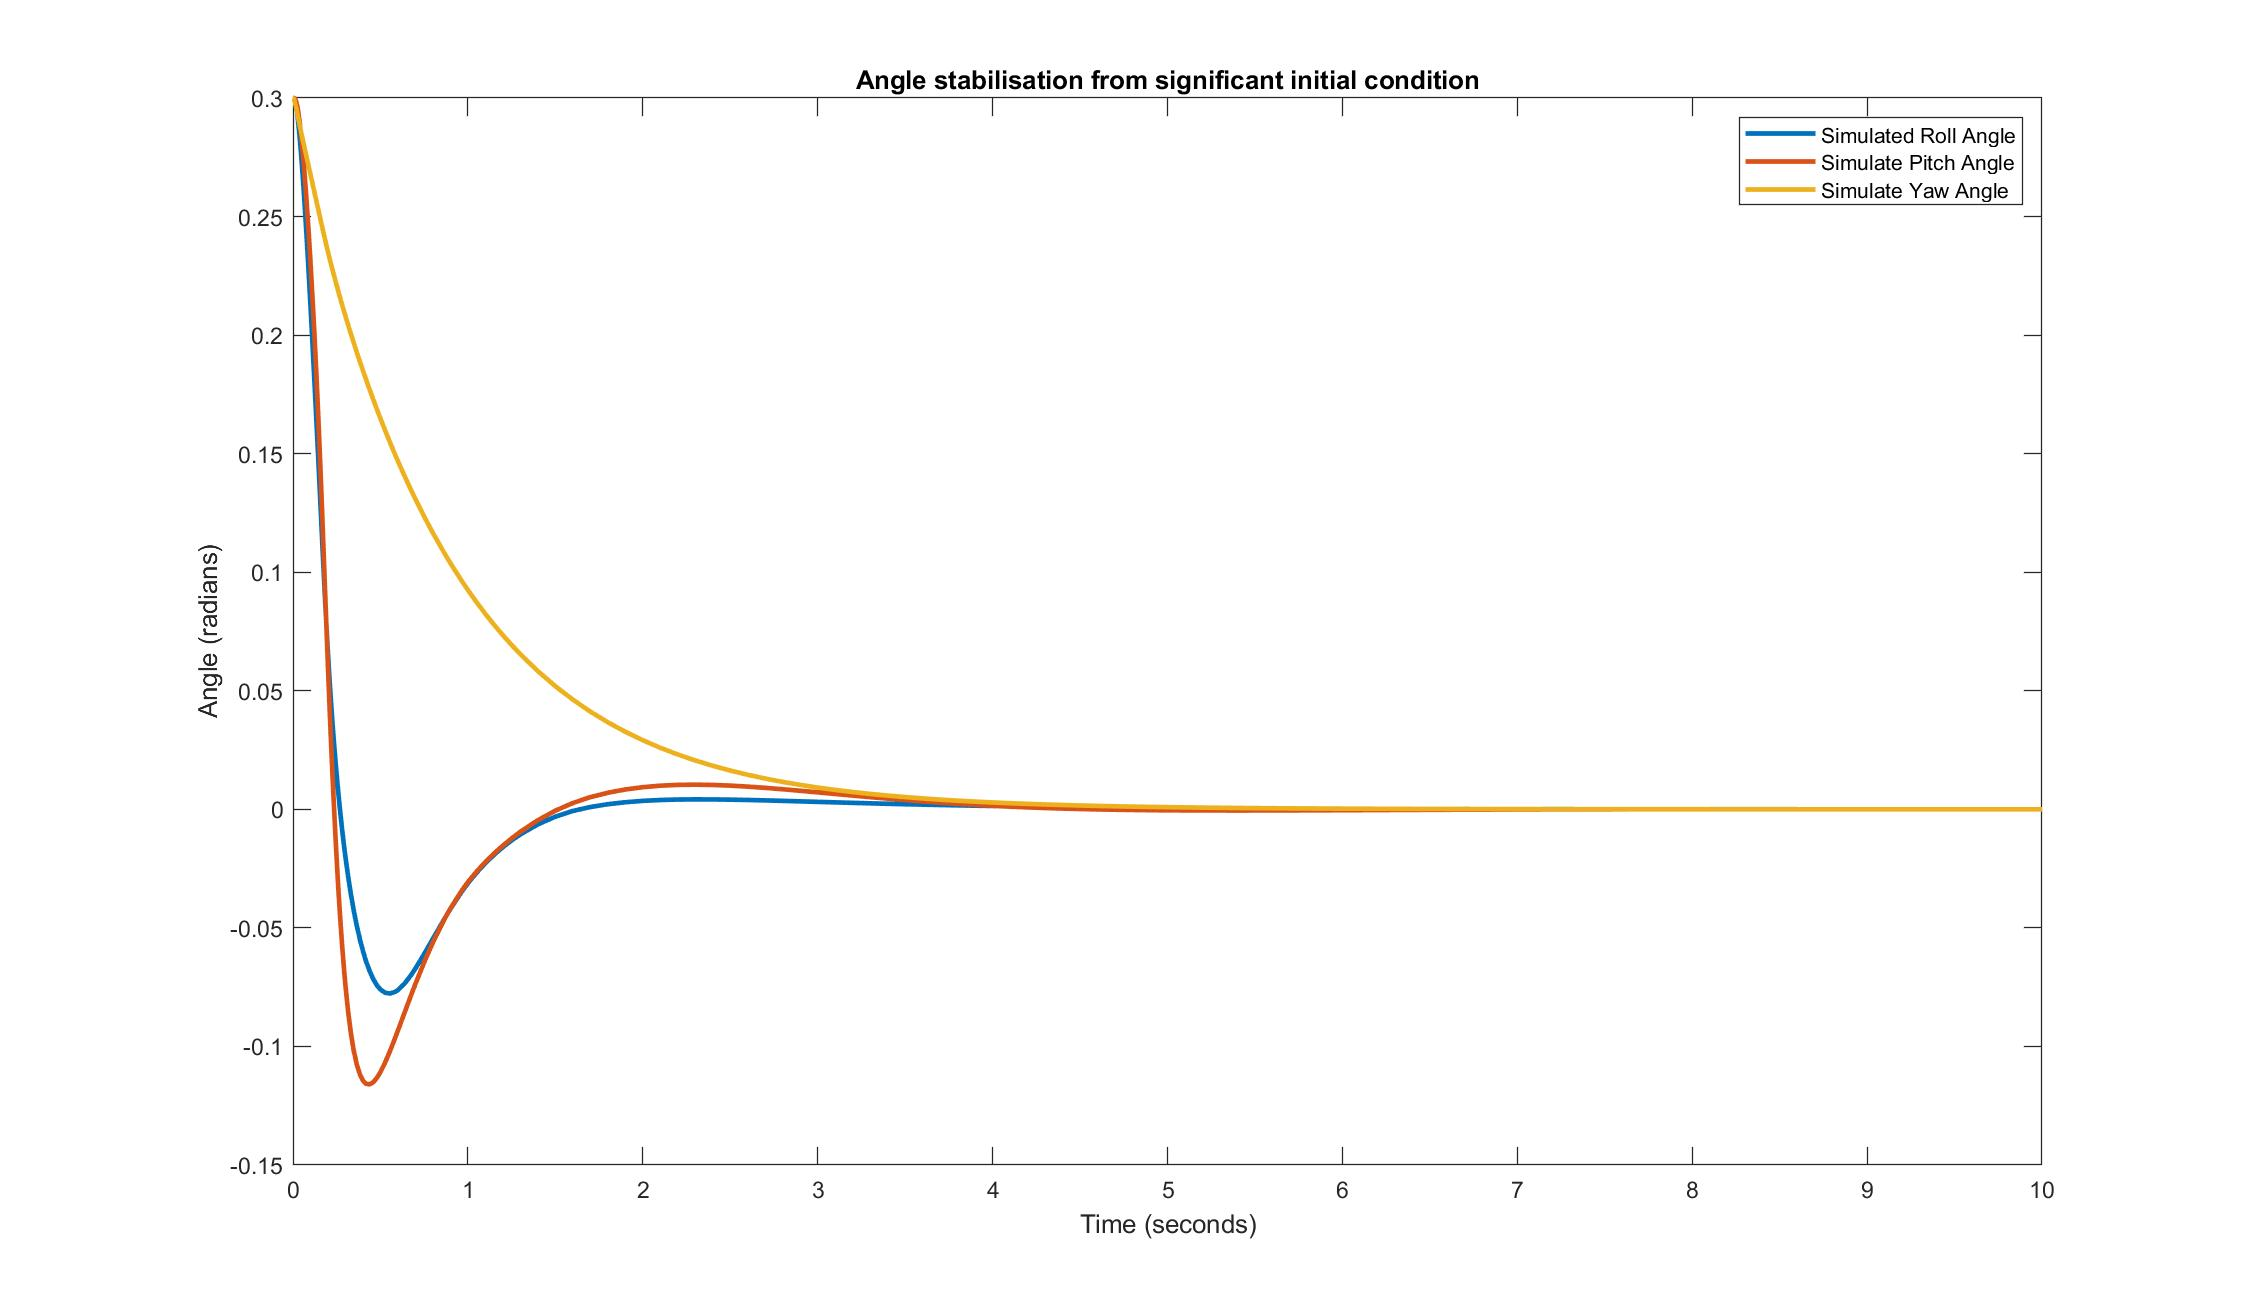
\includegraphics[width=70mm]{/Backstepping_Results/AngleStabilise}
	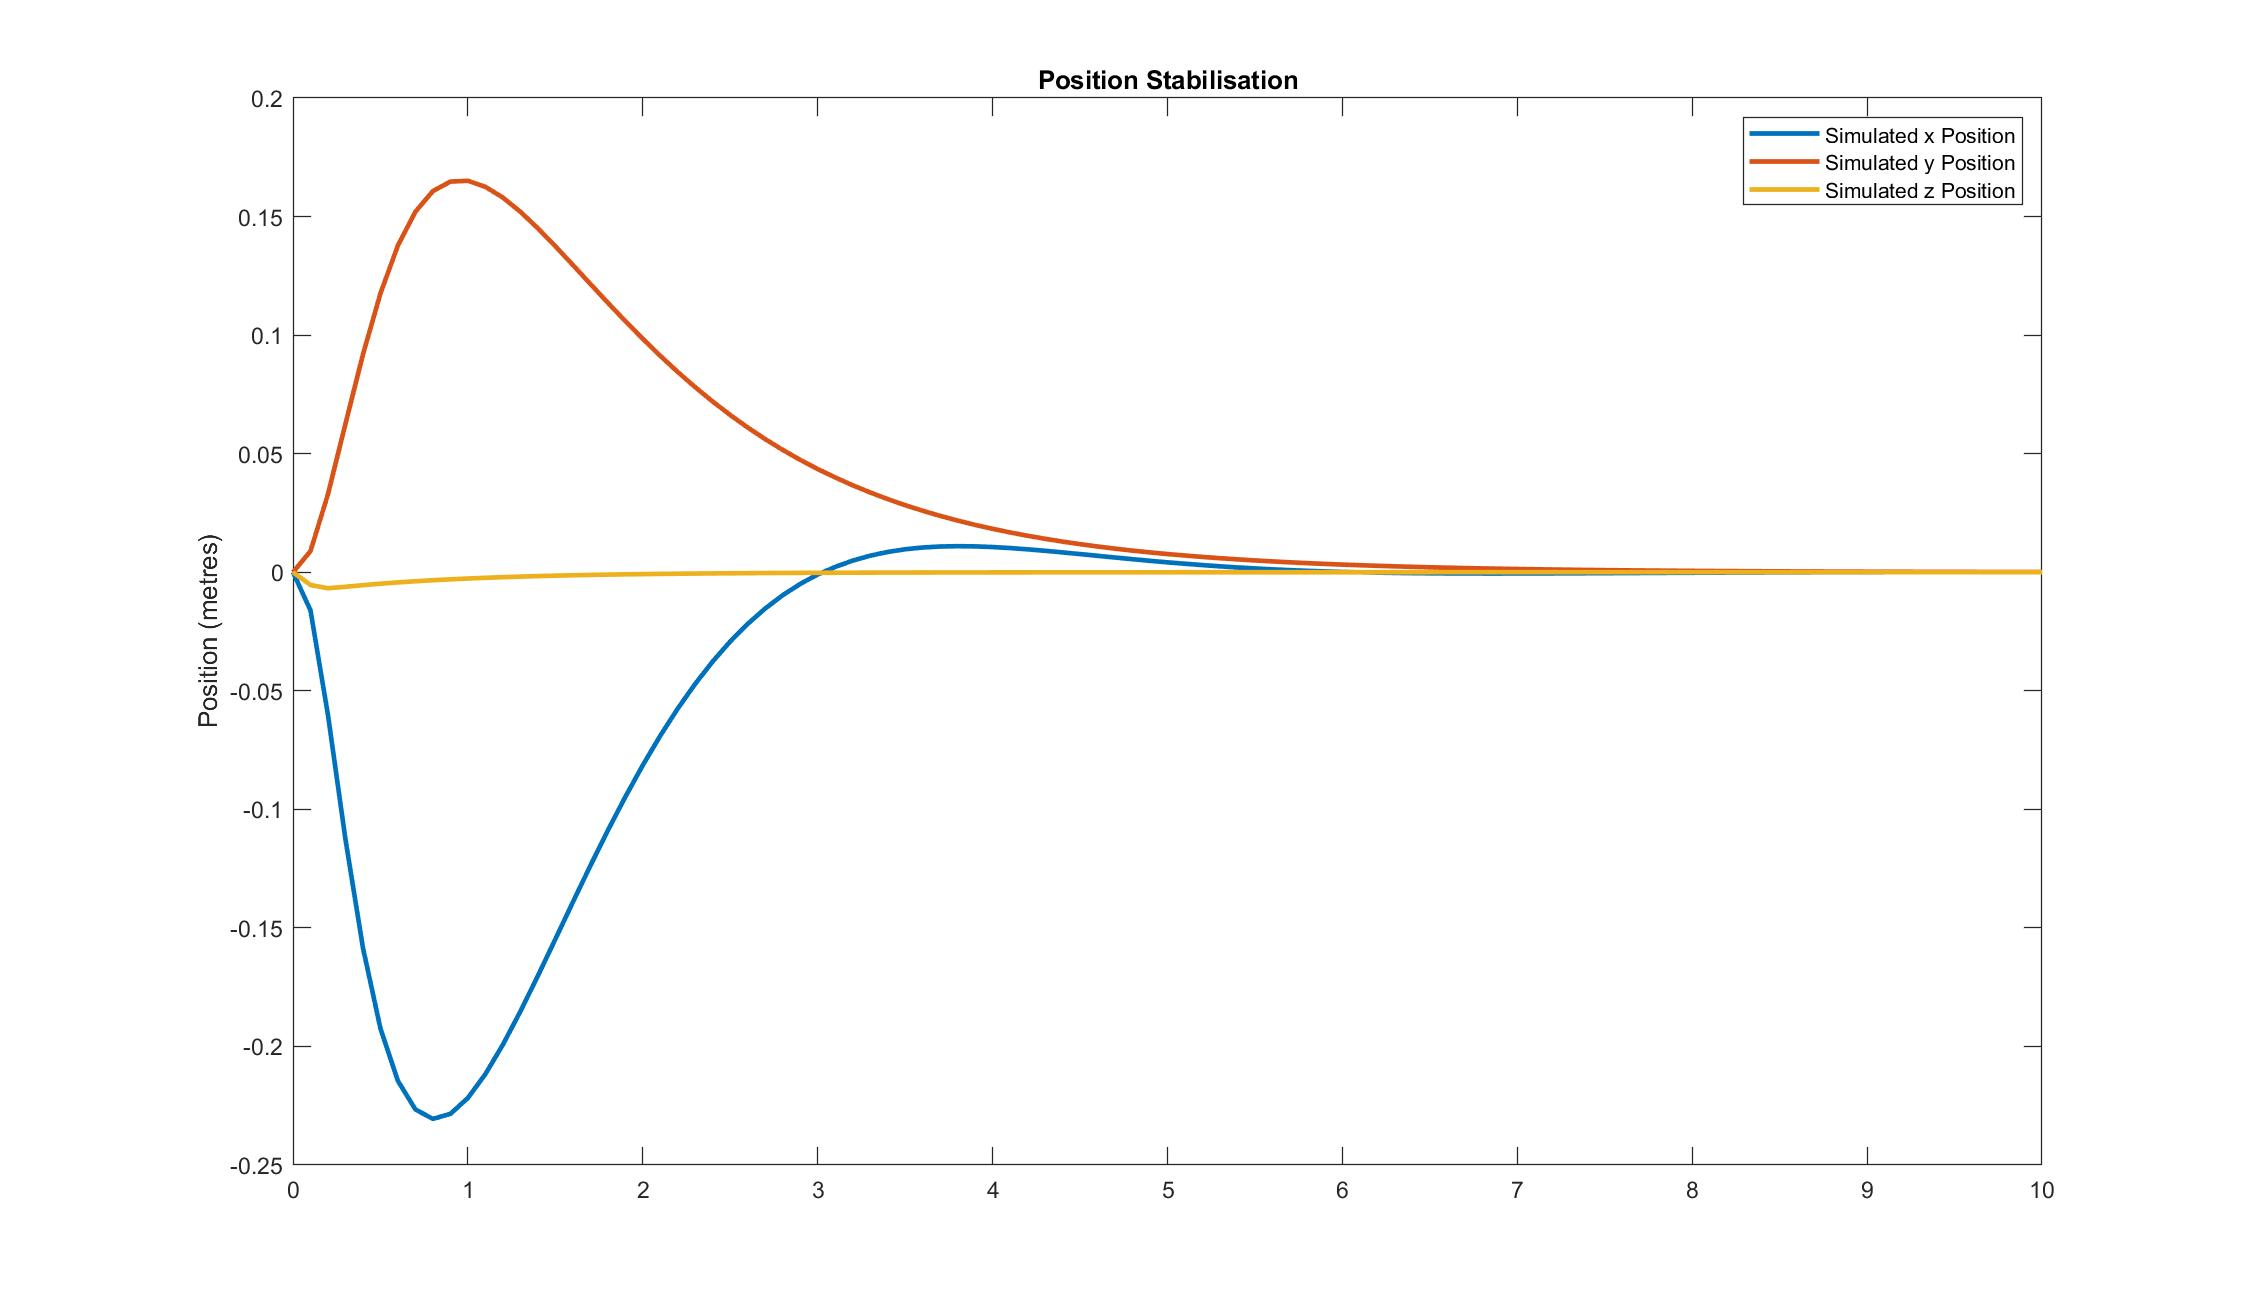
\includegraphics[width=70mm]{/Backstepping_Results/PositionStabilise}%
	\end{center}
	\caption{Backstepping system stabilisation from significant initial angles}%
	\label{fig:Backstepping_Stabilise}%
\end{figure}

\begin{figure}[htb]
\begin{center}
	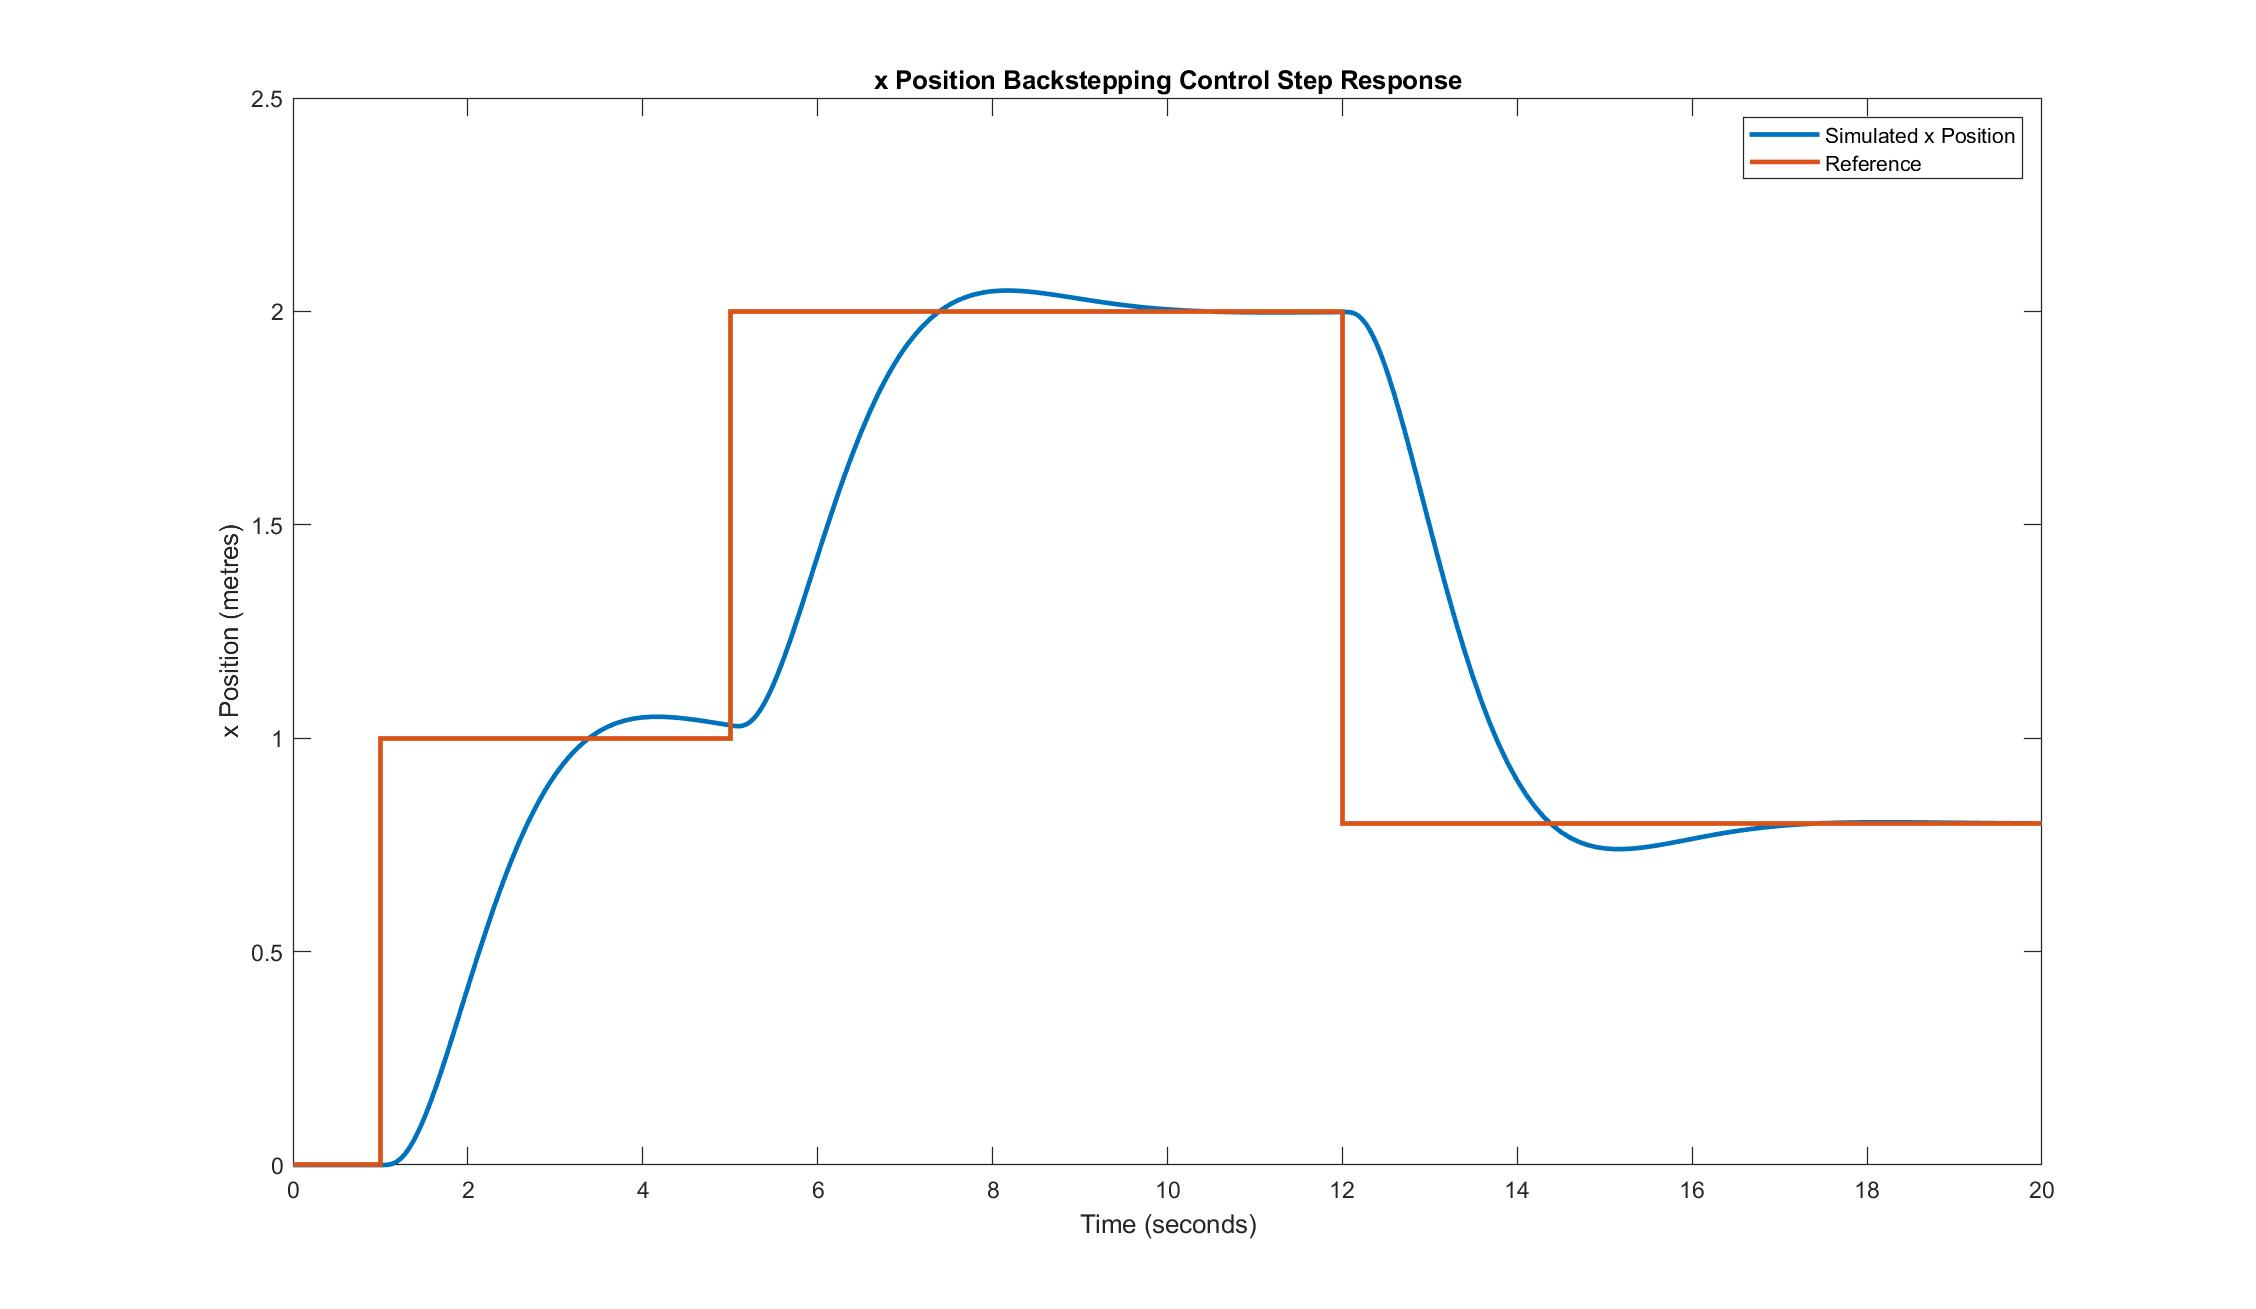
\includegraphics[width=70mm]{/Backstepping_Results/xTracking_Steps1.jpg}%
	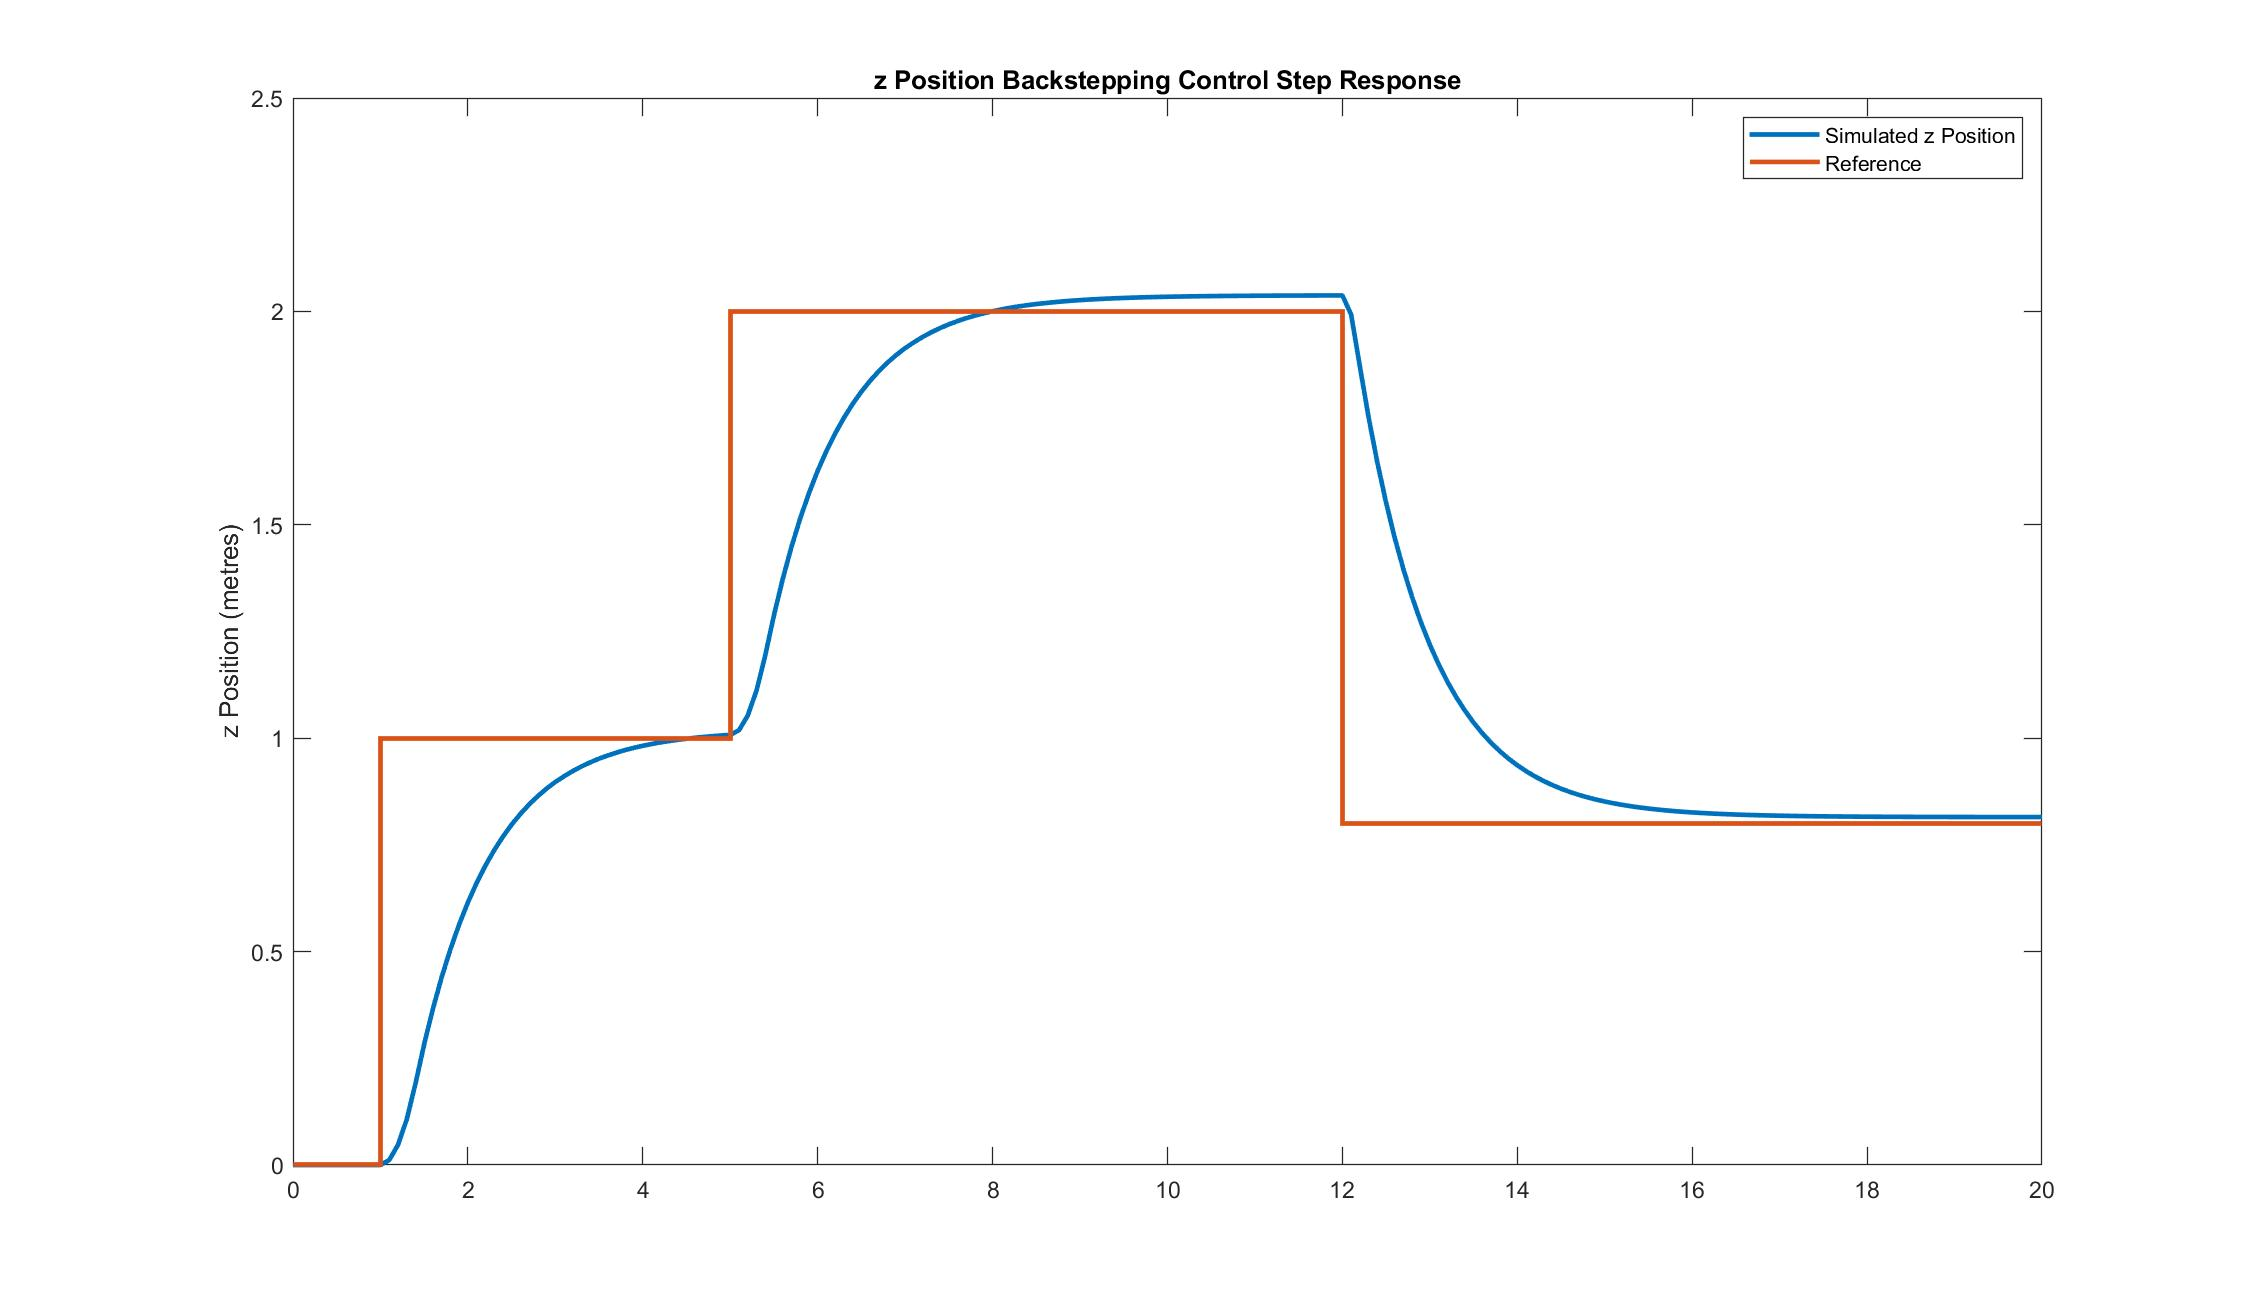
\includegraphics[width=70mm]{/Backstepping_Results/zTracking.jpg}%
	\end{center}
	\caption{Backstepping Position tracking}%
	\label{fig:Backstep_posTrack}%
\end{figure}

\begin{figure}[htb]
\begin{center}
	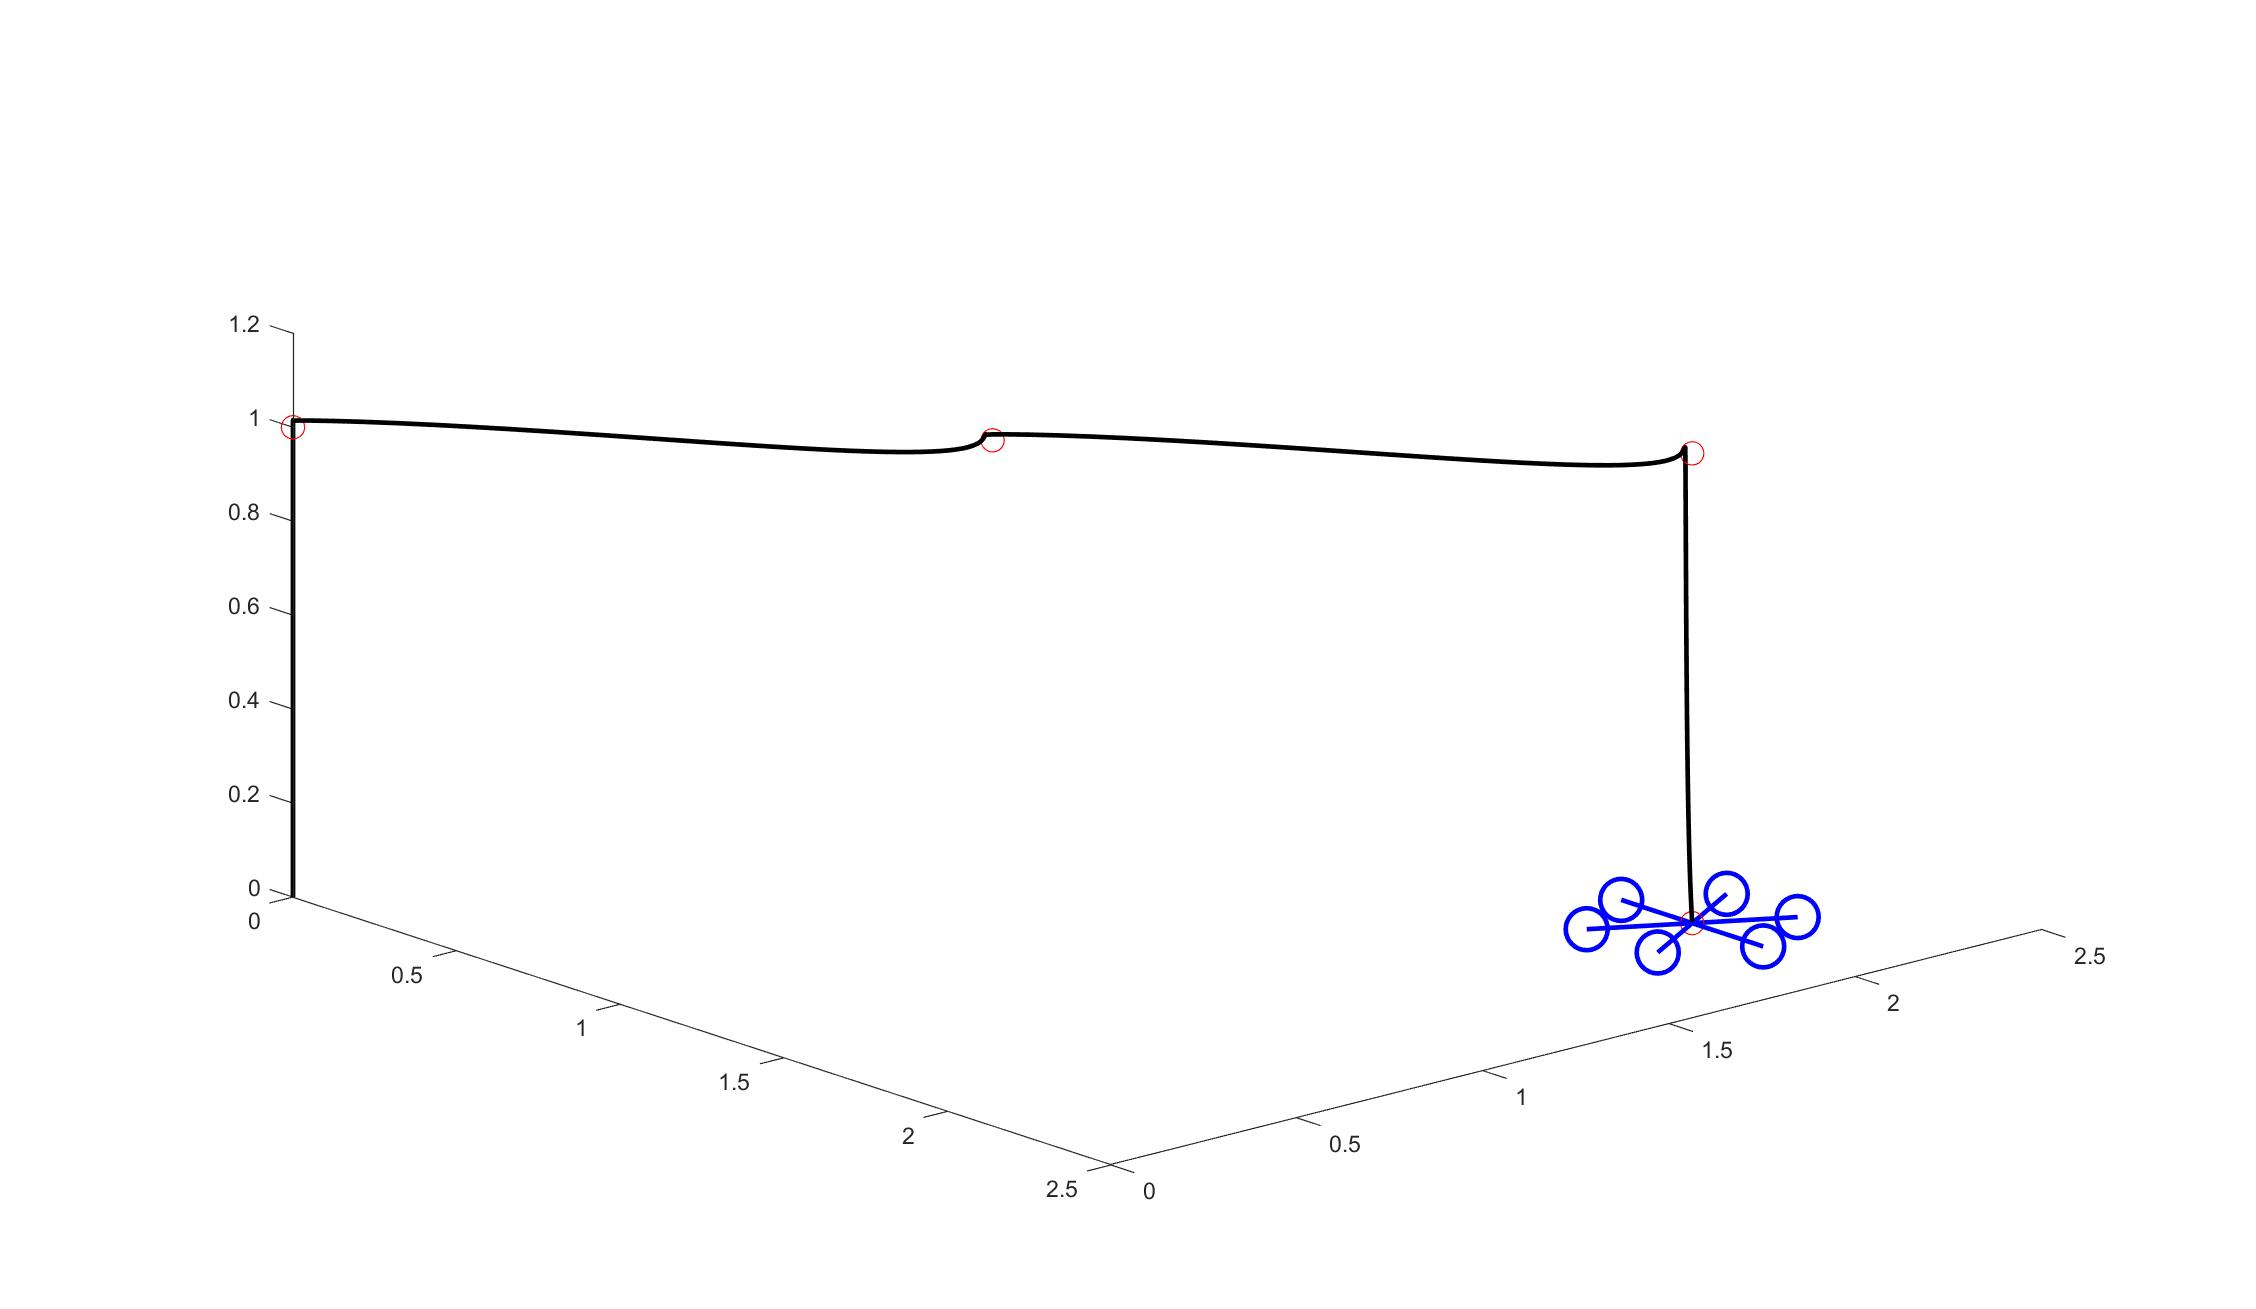
\includegraphics[width=\columnwidth]{/Backstepping_Results/3D_Path_Waypoints2.jpg}%
	\end{center}
	\caption{Backstepping Position tracking}%
	\label{fig:Backstep_path}%
\end{figure}


Show what happens when parameters vary...
\FloatBarrier
\section{Backstepping with Integral Action}\label{section:IntBack}
As an extension, to reduce the effects of uncertainties in model parameters it is desirable to include integral action within the controller. An integral term may thus be added within the negative definite function which is chosen as the time derivative of the candidate Lyapunov function. This method has been shown to be effective at reducing the effects of uncertainties and increasing the robustness of the controller in both simulation\cite{Jasim2015} and hardware\cite{Bouabdallah2006} implementation.

Again, consider the roll angle tracking error as the first translated state:
\[e_{1}=x_{1d}-x_{1}\]
Choose a candidate Lyapunov function such that it is positive definite:
\[V(e_{1})=\frac{1}{2}e_{1}^{2}\]
Taking its derivative gives:
\begin{equation}
\begin{split}
\dot{V}(e_{1})&=e_{1}\dot{e}_{1}\\
\dot{V}(e_{1})&=e_{1}(\dot{x}_{1d}-x_{2})
\end{split}
\end{equation}
Now $\dot{V}(e_{1})$ is chosen equal to a negative definite function which includes an integral term.
\begin{equation}
\begin{split}
\dot{V}(e_{1})&=-C_{1}e_{1}^{2}-e_{1}\beta_{1}\int^{t}_{0} e_{1}(\alpha) d\alpha\\
e_{1}(\dot{x}_{1d}-x_{2})&=-C_{1}e_{1}^{2}-e_{1}\beta_{1}\int^{t}_{0} e_{1}(\alpha) d\alpha\\
\end{split}
\end{equation}
where $C_{1}$ and $\beta_{1}$ are non-negative constants.

A virtual control for roll angle rate ($x_{2}$) is chosen to satisfy this relationship:
\[x_{2d}=\dot{x}_{1d}+C_{1}e_{1}+\beta_{1}\int^{t}_{0} e_{1}(\alpha) d\alpha\]

A control law which stabilises the tracking error $e_{2}=x_{2d}-x_{2}$ can now be derived in terms of the roll torque, using the same method as in the previous section:
\begin{equation}
\tau_{\phi}=\frac{1}{b_{1}} \left( \ddot{x}_{1d}+C_{1}\dot{e}_{1}+\beta_{1}e_{1}+\beta_{2}\int^{t}_{0} e_{2}(\alpha) d\alpha -a_{1}x_{4}x_{6}+C_{2}e_{2}\right)
\end{equation}

Following the same method, control laws for both yaw and pitch angles are given as:
\begin{equation}\label{eqn:IntBackstepAngleLaws}
\begin{split}
\tau_{\theta}&=\frac{1}{b_{2}}\left(\ddot{x}_{3d}+C_{3}\dot{e}_{3}+\beta_{3}e_{3}+\beta_{4}\int^{t}_{0} e_{4}(\alpha) d\alpha -a_{2}x_{2}x_{6}+C_{4}e_{4}\right)\\
\tau_{\psi}&=\frac{1}{b_{3}}\left(\ddot{x}_{5d}+C_{5}\dot{e}_{5}+\beta_{5}e_{5}+\beta_{6}\int^{t}_{0} e_{6}(\alpha) d\alpha -a_{3}x_{2}x_{4}+C_{6}e_{6}\right)
\end{split}
\end{equation}

Similarly to the previous section, virtual controls for the pitch and roll angles can be chosen to stabilise horizontal position tracking errors. Also, a control law for the vertical position can be derived using the total thrust.


\begin{equation}\label{eqn:IntBackPosContLaw}
\begin{split}
x_{3d}&=sin^{-1}\left(\frac{\frac{m}{F_{T}}[C_{8}e_{8}+\beta_{8}\int^{t}_{0} e_{8}(\alpha) d\alpha + \ddot{x}_{7d}+C_{7}\dot{e}_{7}+\beta_{7}e_{7}]-sin(x_{1})sin(x_{5})}{cos(x_{1})cos(x_{5})}\right)\\
x_{1d}&=sin^{-1}\left(\frac{-\frac{m}{F_{T}}[C_{10}e_{10}+\beta_{10}\int^{t}_{0} e_{10}(\alpha) d\alpha +\ddot{x}_{9d}+C_{9}\dot{e}_{9}+\beta_{9}e_{9}]+cos(x_{1})sin(x_{3})sin(x_{5})}{cos(x_{5})}\right)\\
F_{T}&=\frac{m\left(\ddot{x}_{11d}+C_{11}\dot{e}_{11}+\beta_{11}e_{11}+C_{12}e_{12}+\beta_{12}\int^{t}_{0} e_{12}(\alpha) d\alpha +g\right)}{cos(x_{1})cos(x_{3})}
\end{split}
\end{equation}


\subsection{Preliminary Results}
Show effects of saturation...

\section{Actuator Saturation}
To prevent actuator saturation when large step commands are given, a sigmoidal function can be used to limit the effect of position error \cite{Cabecinhas2009}. For this purpose, the sigmoidal function is defined as:
\[\sigma(x)=p_{max}\frac{x}{1+|x|}\]



\section{Chapter Summary}
In this chapter, three control systems were developed and tested in simulation. The PID control system was effective at stabilising the aircraft around a hovering point, but had limitations due to not considering the nonlinearities of the system. The backstepping control system improved upon this by accounting for the nonlinearities, however this controller still depended on accurate values of the model parameters. The final controller implemented backstepping control with integral action and was effective in adjusting to errors in the given model parameters, however it was prone to actuator saturation with large step commands. The final addition to the control system implemented a sigmoidal function in the position control laws to mitigate the effects of actuator saturation.



\clearpage





\chapter{State Estimation and Sensor Fusion}
\textit{This chapter describes the algorithms used for estimating the aircraft state from the available sensor readings. It is common for state estimation algorithms to rely on GPS systems for position data, however there are many situations where GPS may either be unavailable or unreliable. This chapter explores a state estimation technique which utilises an optical flow sensor for relative position data. This is then compared with a GPS-enabled algorithm.}

\section{Filter Algorithm}\label{section:Filter}
The algorithm chosen to fuse sensor data and estimate states is based upon an Extended Kalman Filter (EKF). The fundamentals of EKFs are discussed in Section \ref{section:EKFBackground}. The measurement functions will be slightly different for each of the two following algorithms, as these functions are dependent on the sensors being used. However, the state transition functions are common to both algorithms. 

\subsection{State Transition Functions}\label{section:StateTrans}
The model developed in Chapter \ref{chapter:Modelling} could theoretically be used in defining the state transition functions of the system. However, this would require knowing the torque values around each axis and the total thrust produced by the propeller in real-time. In practice, accurate values for these inputs are not easily measured. Therefore, a separate model is used by considering body-fixed acceleration and angular rates as the inputs.

The states estimated by this EKF are those used by the backstepping controller, as expressed in \eqref{eqn:stateDef}. Namely, the positions, velocities, Euler angles and angular rates all expressed with respect to the Earth frame.In order to simplify notation, the states may be grouped into the following 4 vectors: \textbf{\textit{p}}$=\begin{bmatrix}x& y& z\end{bmatrix}^{T}$, \textbf{\textit{v}}$=\begin{bmatrix}\dot{x}& \dot{y}& \dot{z}\end{bmatrix}^{T}$, \textbf{\textit{$\Phi$}}$=\begin{bmatrix}\phi& \theta& \psi\end{bmatrix}^{T}$ and \textbf{\textit{$\omega$}}$=\begin{bmatrix}\dot{\phi}& \dot{\theta}& \dot{\psi}\end{bmatrix}^{T}$. Both algorithms will utilise accelerometer and gyroscope measurements and these measurements are defined as inputs in order to reduce the complexity of the state transition functions \cite{Driessen2018}. Thus the inputs are $\textbf{\textit{u}}=
\begin{bmatrix}
\tilde{a}_{x}&\tilde{a}_{y}&\tilde{a}_{z}&\tilde{\omega}_{x}&\tilde{\omega}_{y}&\tilde{\omega}_{z}
\end{bmatrix}^{T}
$. The state transition functions used for the prediction step of the EKF are defined in discrete time:
\begin{equation}\label{eqn:OFS_EKFStateTrans}
\begin{split}
\textbf{\textit{p}}_{k+1}&=\textbf{\textit{p}}_{k}+\Delta t\textbf{\textit{v}}_{k} \\
\textbf{\textit{v}}_{k+1}&=\textbf{\textit{v}}_{k}+\Delta t\left( C^{n}_{b}
\begin{bmatrix}
u_{1}\\
u_{2}\\
u_{3}
\end{bmatrix}
+
\begin{bmatrix}
0\\
0\\
g
\end{bmatrix}
\right)\\
\textbf{\textit{$\Phi$}}_{k+1}&=\textbf{\textit{$\Phi$}}_{k}+\Delta t\textbf{\textit{$\omega$}}_{k}\\
\textbf{\textit{$\omega$}}_{k+1}&=
\begin{bmatrix}
1& sin(\phi)tan(\theta)& cos(\phi)tan(\theta)\\
0 &cos(\phi) &-sin(\phi)\\
0 &sin(\phi)sec(\theta) &cos(\phi)sec(\theta)
\end{bmatrix}
\begin{bmatrix}
u_{4}\\
u_{5}\\
u_{6}
\end{bmatrix}
\end{split}
\end{equation}
 

\section{State Estimation with GPS}\label{section:GPS_EKF}
In industry and commercial applications UAV position is commonly estimated with the use of a GPS sensor, along with additional sensors. This method has the advantage of providing accurate position data that not many other sensors can offer.

\subsection{Sensor Models}\label{section:GPS_sensorModels}
GPS data is recorded as latitude and longitude positions. These can be converted into the Earth frame by using the Haversine formula, as described in Section \ref{section:RefFrames}. The GPS data will be modelled by the following:
\begin{equation}
\begin{split}
\tilde{\lambda}&=\lambda+\mu_{\lambda}\\
\tilde{\chi}&=\chi +\mu_{\chi}
\end{split}
\end{equation}
where $\lambda$ and $\chi$ represent latitude and longitude respectively and the $\mu$ terms represent measurement noise

A standard Inertial Measurement Unit (IMU) contains both a 3-axis accelerometer and a 3-axis gyroscope. These sensors are modelled by the following equations:
\begin{equation}\label{eqn:IMU}
\begin{split}
\begin{bmatrix}
\tilde{a}_{x}\\
\tilde{a}_{y}\\
\tilde{a}_{z}
\end{bmatrix}
&=
\begin{bmatrix}
\dot{u}\\
\dot{v}\\
\dot{w}
\end{bmatrix}
+
C^{b}_{n}
\begin{bmatrix}
0\\
0\\
g
\end{bmatrix}
+
\begin{bmatrix}
\mu_{a_{x}}\\
\mu_{a_{y}}\\
\mu_{a_{z}}
\end{bmatrix}\\
\begin{bmatrix}
\tilde{\omega}_{x}\\
\tilde{\omega}_{y}\\
\tilde{\omega}_{z}
\end{bmatrix}
&=
\begin{bmatrix}
p\\
q\\
r
\end{bmatrix}
+
\begin{bmatrix}
\mu_{\omega_{x}}\\
\mu_{\omega_{y}}\\
\mu_{\omega_{z}}
\end{bmatrix}
\end{split}
\end{equation}

A magnetometer is another commonly used sensor in inertial navigation systems. The magnetometer measures the Earth's magnetic field in order to estimate vehicle orientation. The measurements can be modelled by the following:
\begin{equation}\label{eqn:mag}
\begin{bmatrix}
\tilde{m}_{x,b}\\
\tilde{m}_{y,b}\\
\tilde{m}_{z,b}
\end{bmatrix}
=
C^{b}_{n}
\begin{bmatrix}
m_{x}\\
m_{y}\\
m_{z}
\end{bmatrix}
+
\begin{bmatrix}
\mu_{m_{x}}\\
\mu_{m_{y}}\\
\mu_{m_{z}}
\end{bmatrix}
\end{equation}
Where $m_{x}$, $m_{y}$ and $m_{z}$ represent the magnetic field vector components at the vehicle's location, and $\tilde{m}_{x,b}$, $\tilde{m}_{y,b}$ and $\tilde{m}_{z,b}$ are the magnetometer measurements in the vehicle body frame. To perform orientation determination, a known magnetic field vector at the location of the vehicle is required. For the purposes of this project, it will be assumed that the vehicle is flying outdoors without significant magnetic interference nearby, i.e. the Earth's magnetic field is the only magnetic field detected.\\

A barometer (or altimeter) is a sensor which measures air pressure and can be used to estimate relative altitude. The model for a barometric sensor is based upon the standard atmospheric model described in Section \ref{section:barometerBackground}. This sensor model is given in \eqref{eqn:barometer}.
\begin{equation}\label{eqn:barometer}
\tilde{P}=P_{0}exp\left[\frac{-g M (z+h_{0})}{R T_{0}}\right]+\mu_{P}
\end{equation}

where $\tilde{P}$ represents the measured pressure. In the model, z represents the height above the surface from which it launched, thus $h_{0}$ is added to account for the surface's altitude above sea level.


\subsection{Preliminary Results}
The EKF was tested in simulation with a number of steps in the x direction and a single step in the z direction. In these results, the control system developed in Chapter \ref{chapter:control} is used. The controller is provided with the actual states rather than the estimated states. Additionally, the sample rate of all sensors is assumed to be 100 Hz.\\

The estimated states are compared with the actual states in \figref{fig:GPS_EKF_Results}. The angular rates and translational positions are estimated accurately, however there is some error in the translational velocities and Euler angle estimates. None of the measurement functions directly involve the velocity states, therefore they are essentially estimated based upon the state transition functions alone, which limits the accuracy of the estimates. The Euler angles are included in both the magnetometer and accelerometer functions in the form of the rotation matrix ($C_{n}^{b}$). However, the measurement functions do not directly measure the angles, i.e. there are terms such as $cos(\phi)sin(\phi)cos(\psi)$ within the function. This results in the estimated angles being correlated, i.e. a change in $\theta$ results in the estimates for $\phi$ and $\psi$ also being affected.

\begin{figure}[htb]
\begin{center}
	\includegraphics[width=\columnwidth]{/EKF_GPS/xSteps_Angles.jpg}\\
	\includegraphics[width=\columnwidth]{/EKF_GPS/xSteps_Positions.jpg}
	\end{center}
	\caption{Estimated states using GPS extended Kalman filter.}%
	\label{fig:GPS_EKF_Results}%
\end{figure}


\FloatBarrier
\section{State Estimation without GPS}
There are many situations in which GPS signal may not be reliable. For example, GPS signal will generally be unreliable for indoor applications. Additionally, failure of the onboard GPS system could prove catastrophic if there is not another way of tracking position and velocity data.
\subsection{Sensor Models}\label{section:GPSSensModels}
One type of sensor which is relatively inexpensive and can be utilised for position tracking in GPS-limited environments, is the optical flow sensor (OFS). An OFS is essentially a simple camera which compares consecutive frames to establish the motion that has occurred between frames. The OFS outputs data relating to the flow of pixels between frames. The velocity in m/s can be estimated by combining this with knowledge of the scene depth, i.e. the distance from the surface. In most cases, an OFS will be accompanied by either a lidar or sonar sensor in order to estimate scene depth. For the purposes of this model, the z position of the aircraft represents its height above the ground, which implies the terrain within the flight path is flat. The optical flow sensor and its accompanying lidar sensor are modelled by the following equations\cite{Driessen2018}\cite{Ding2010}:


\begin{equation}\label{eqn:OFS}
\begin{split}
\tilde{\rho}_{x}=-\left(\frac{u}{h}+q\right)\Delta t_{\rho}f+\mu_{\rho_{x}}\\
\tilde{\rho}_{y}=-\left(\frac{v}{h}+p\right)\Delta t_{\rho}f+\mu_{\rho_{y}}\\
\tilde{h}=\frac{z}{cos(\phi)cos(\theta)}+\mu_{h}
\end{split}
\end{equation}
where $\Delta t_{\rho}$ is the time between consecutive frames, $f$ is the focal length in pixels, $h$ is the scene depth and $\mu$ variables represent Gaussian noise with zero mean.\\
This algorithm also uses the IMU and magnetometer sensor models described in Section \ref{section:GPSSensModels}, but does not use the GPS or barometer.

\subsection{Preliminary Results}

This algorithm was tested in simulation using the same input reference as the previous algorithm. The results are shown in \figref{fig:EKF_OFS_Results}. It can be seen that the results are comparative to the previous GPS-enabled algorithm. The x and y velocity estimates are more accurate since these are measured by the optical flow sensor. However, the x and y position estimates are prone to drift, as the sensors do not directly measure these states. Also, the further the aircraft is above the surface, the larger the effect of noise on the velocity readings. This effect may make this method inappropriate for use at high altitudes. 

\begin{figure}[htb]
\begin{center}
	\includegraphics[width=\columnwidth]{/EKF_OFS/xSteps_Angles.jpg}\\
	\includegraphics[width=\columnwidth]{/EKF_OFS/xSteps_Positions.jpg}
	\end{center}
	\caption{Estimated states using OFS extended Kalman filter.}%
	\label{fig:EKF_OFS_Results}%
\end{figure}

\figref{fig:EKF_OFS_Drift} shows the estimated translational states while the vehicle hovers at a fixed point 10 meters above the origin. This demonstrates the drift of position estimates. However, over 1000 seconds the drift is limited to approximately $\pm$0.25 metres. If there is significant sensor bias, i.e. the noise has a non-zero mean, this drift could become more significant.
\begin{figure}[htb]
\begin{center}
	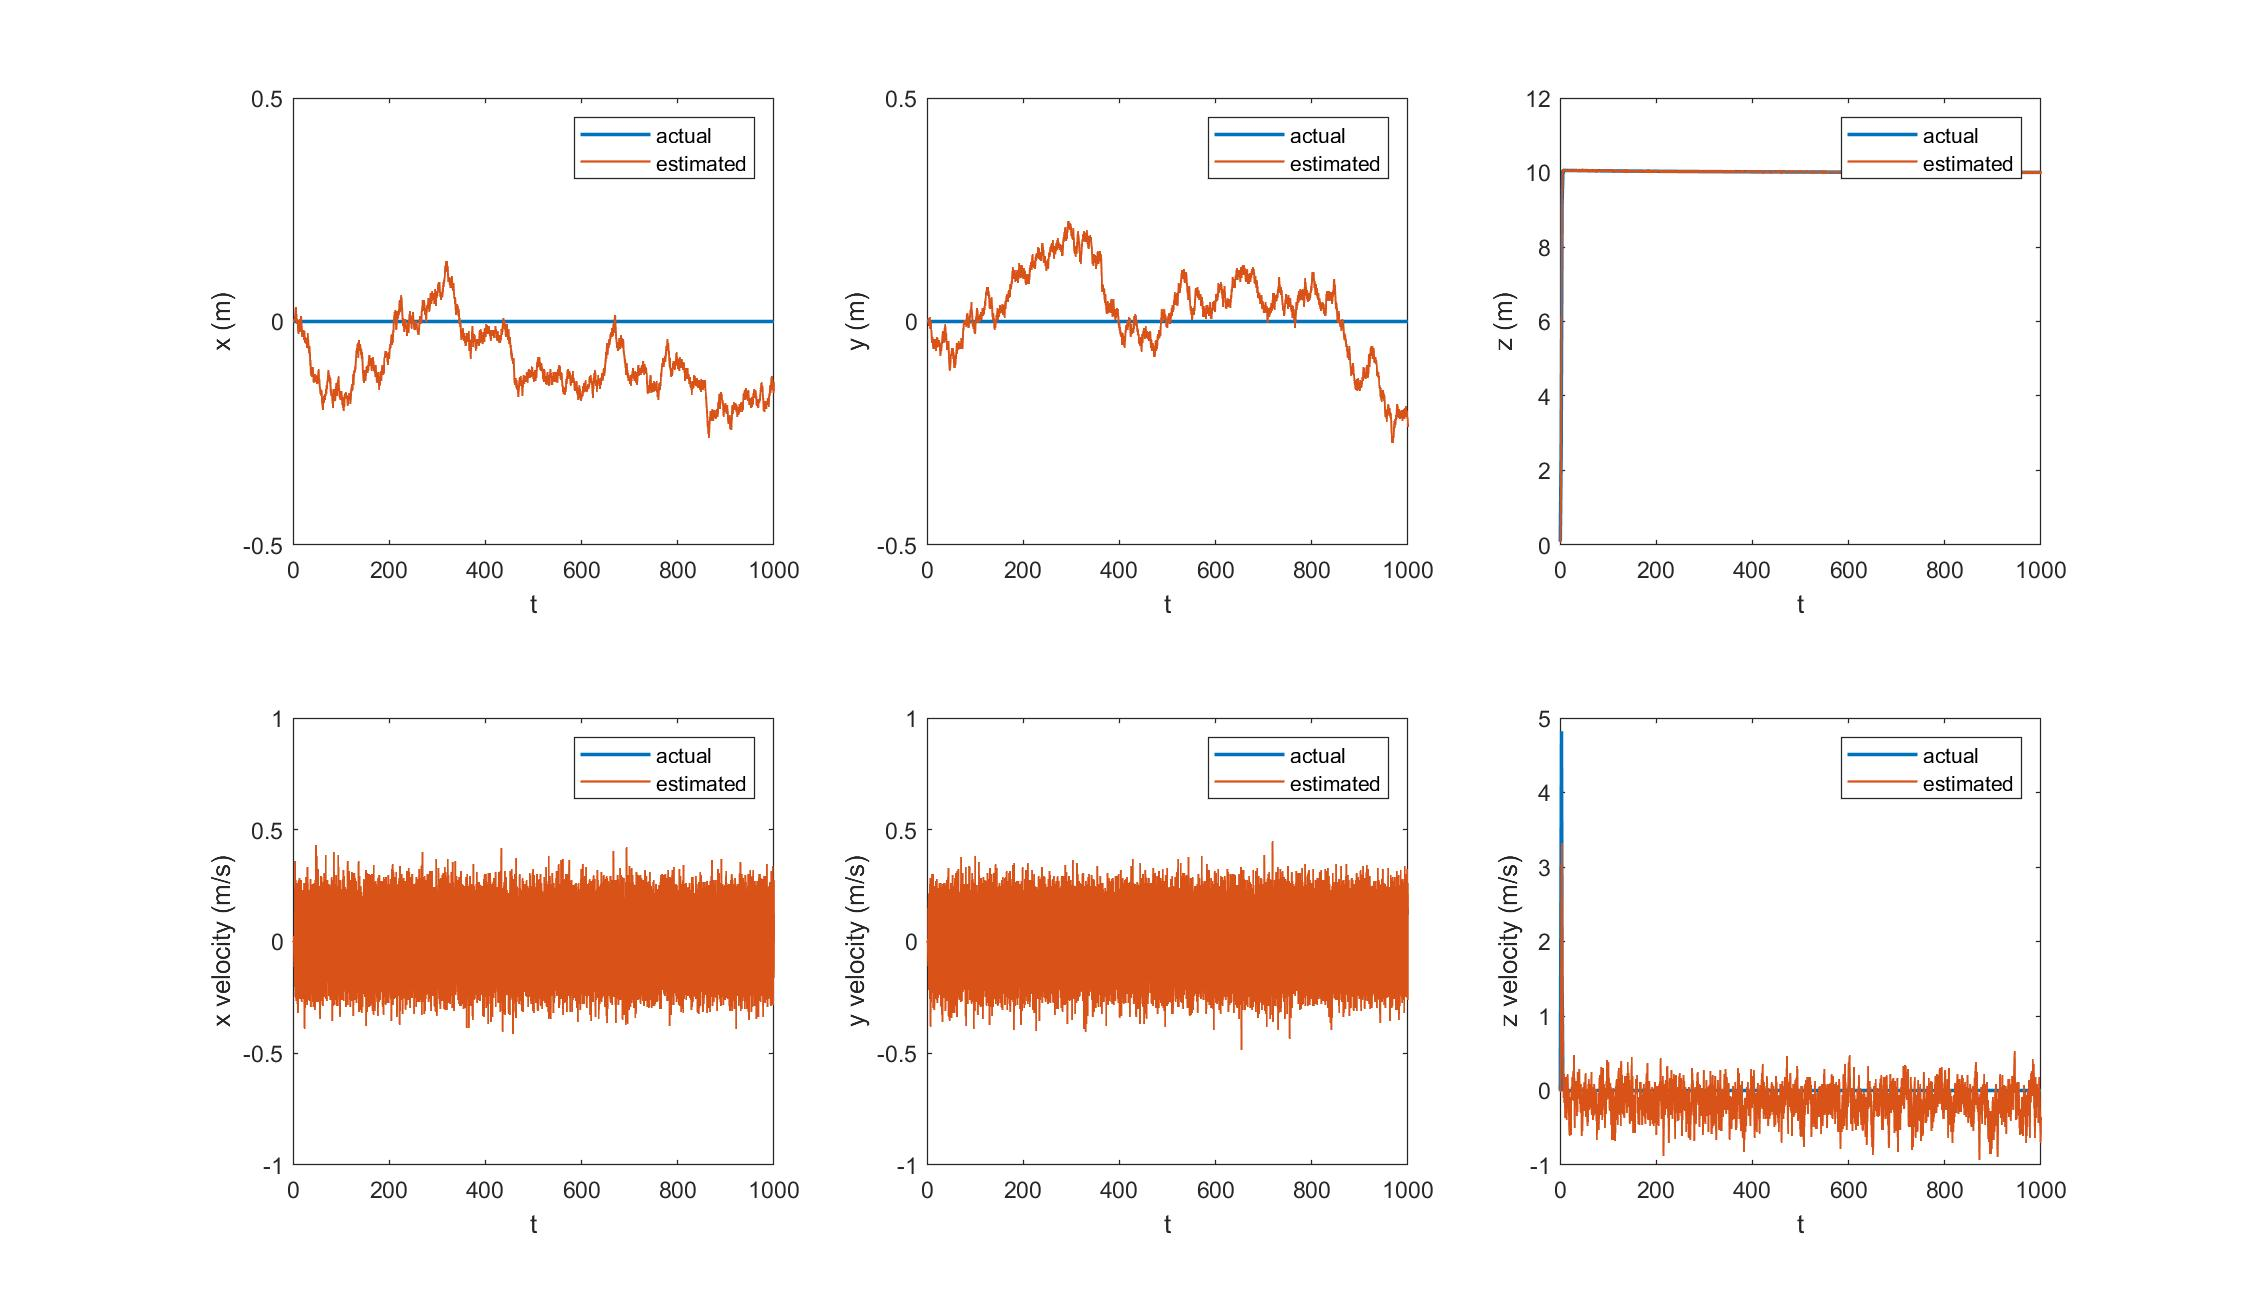
\includegraphics[width=\columnwidth]{/EKF_OFS/Drift.jpg}\\
	\end{center}
	\caption{Estimated translational states over 1000 seconds.}%
	\label{fig:EKF_OFS_Drift}%
\end{figure}

\figref{fig:EKF_OFS_3D} visually compares the vehicle's simulated position with its estimated position in 3D space, whilst moving between a number of waypoints. It can be seen that, although there is no GPS data available a fairly accurate position estimate can be maintained even whilst the vehicle is tracking waypoints.
\begin{figure}[htb]
\begin{center}
	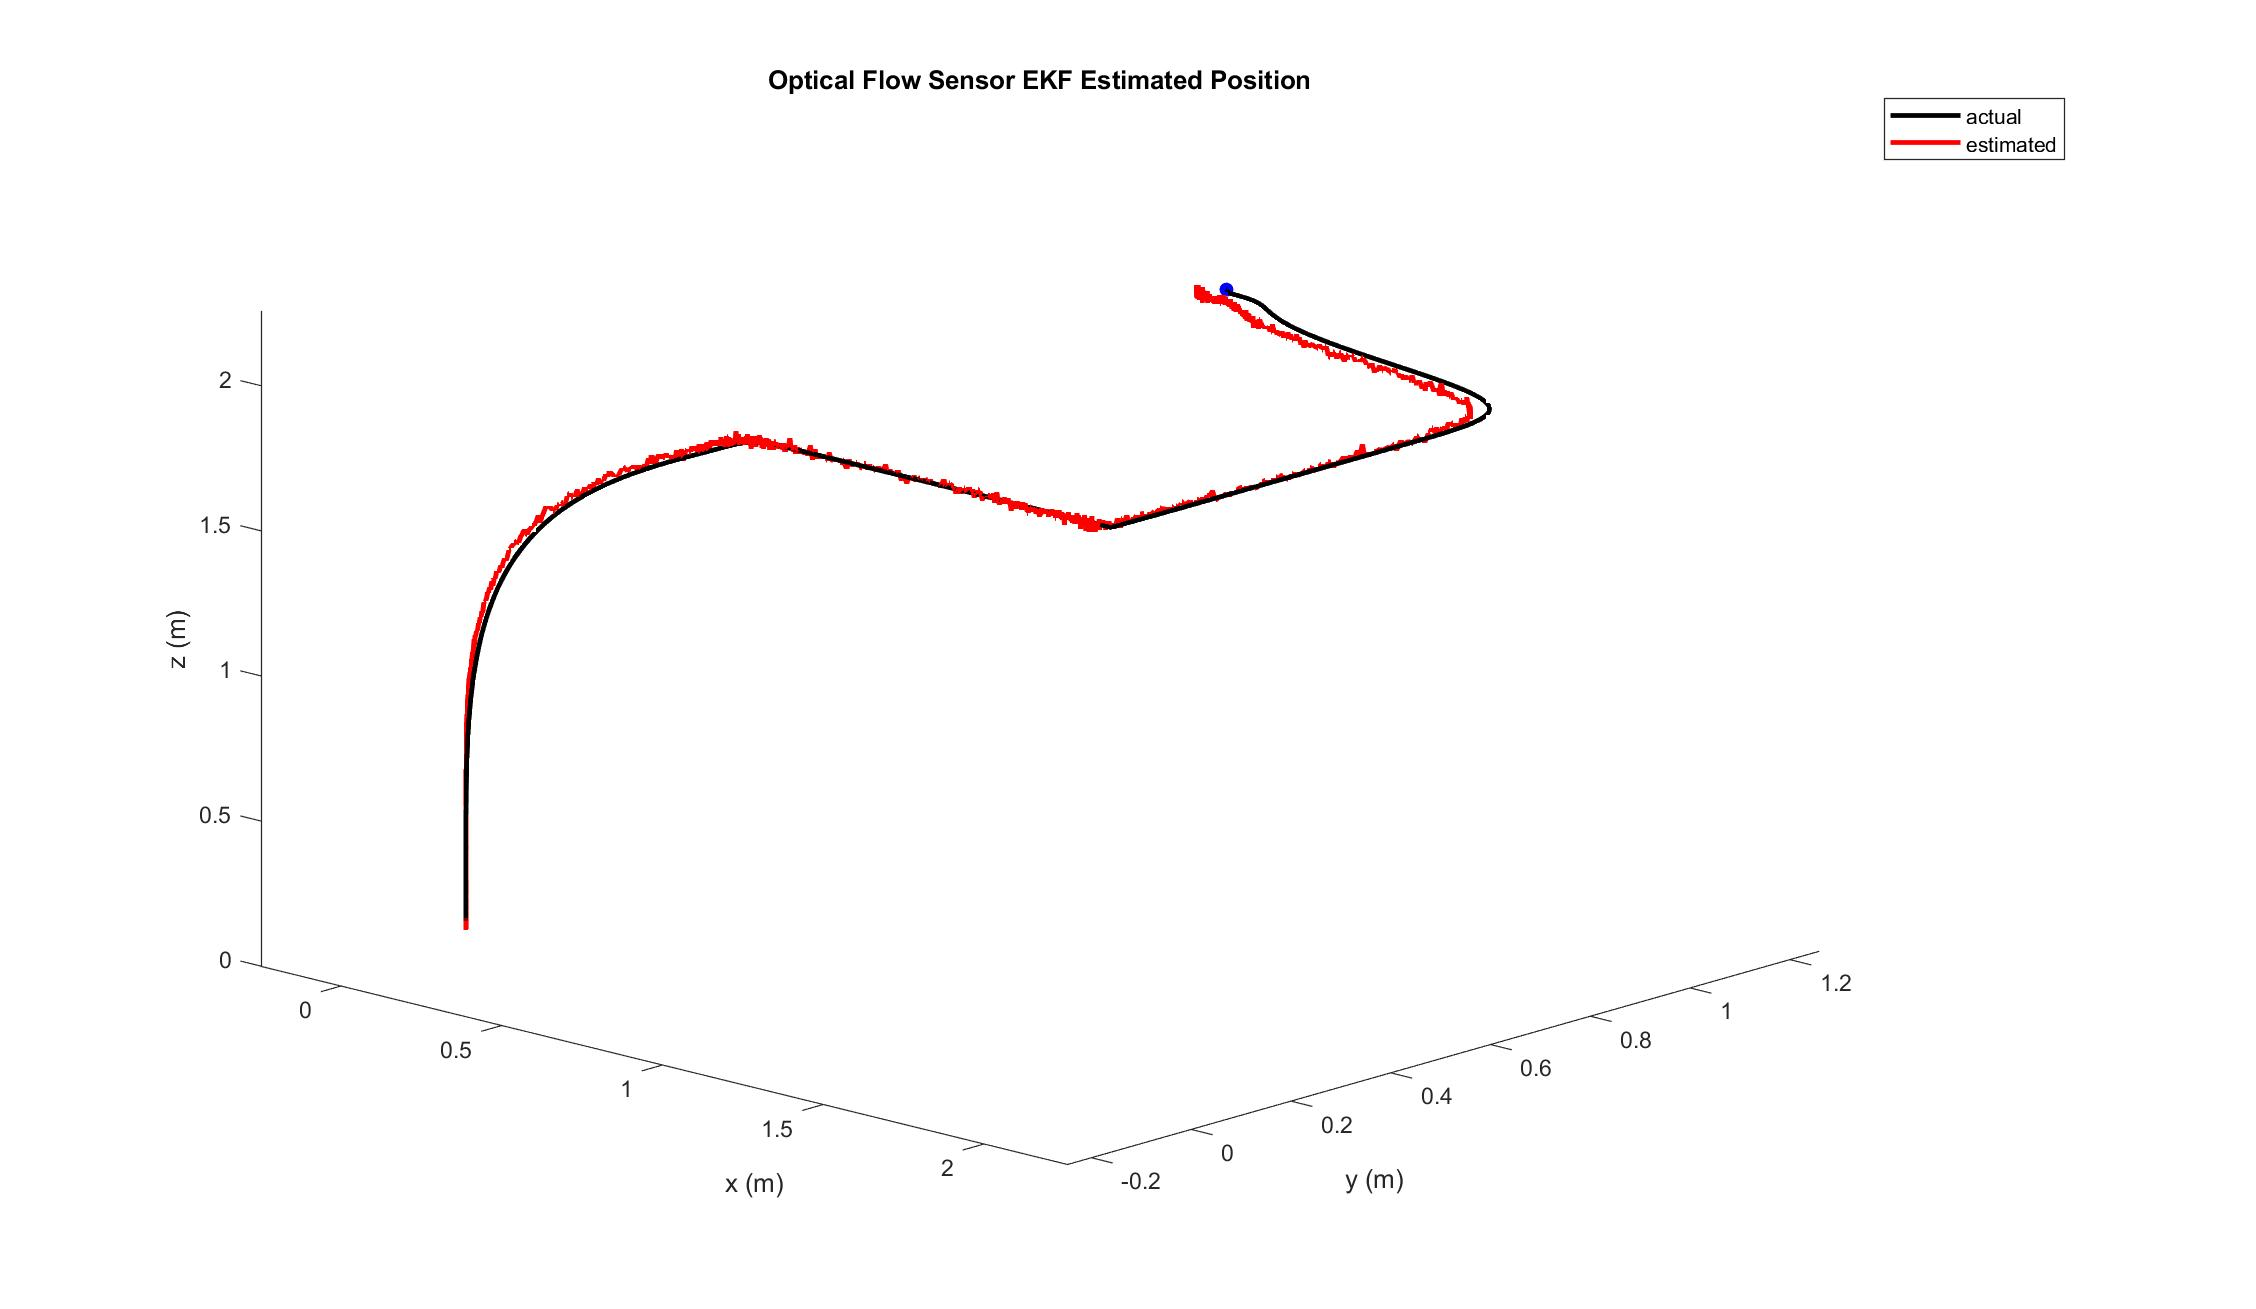
\includegraphics[width=\columnwidth]{/EKF_OFS/Waypoints.jpg}\\
	\end{center}
	\caption{Estimated position of the vehicle in 3D space while moving between waypoints over a period of 20 seconds.}%
	\label{fig:EKF_OFS_3D}%
\end{figure}


A more accurate and reliable EKF would utilise all of the previously mentioned sensors i.e. GPS, barometer, OFS and lidar. 

\FloatBarrier

\section{Chapter Summary}
This chapter developed two sensor fusion algorithms based on the extended Kalman filter. The first algorithm utilises GPS data to estimate position. The second estimator utilises an optical flow sensor and does not rely on GPS. This has the advantage of allowing UAV operation in areas which have limited GPS signal, but is limited to operating with unobstructed line of sight to the ground. A more reliable sensor fusion algorithm would include the use of both groups of sensors. The next chapter will implement these algorithms with real sensor data gathered from test flights of a UAV platform.

\clearpage



%
\chapter{Path-Following}

\section{}


\section{Chapter Summary}
\clearpage




\chapter{Implementation}\label{chapter:Implementation}
\textit{This chapter outlines the specifications of the hardware platform to be used for flight testing. The state estimation algorithms developed in the previous chapter are now tested using sensor data from a number of flight tests. }


\section{Hardware}\label{section:Hardware}
%Verify EKF using Hardware
%Description of the Hardware
%Pixhawk 2.1 CubeBlack, Intel Edison, APSync, Ardupilot ArduCopter 4.1. 
%Sensors onboard the Cube, plus OFS and GPS external sensors.

In addition to the simulation results, test flights were conducted with a custom hexacopter with the aim of collecting data to verify the EKF algorithms. The hexacopter frame is based upon a commercially available kit known as the Storm Drone 6, along with a custom PCB structure for power distribution. Power is supplied by a 5500 mAh 3S Lithium Polymer (LiPo) battery with a nominal voltage of 11.1 V. The battery voltage is regulated at 5 V to supply the flight controller. The propellers are driven by 1260 kv brushless DC motors. The speed of the motors is controlled by a pulse width modulation (PWM) signal supplied to the associated electronic speed controllers (ESC). The UAV platform is shown in \figref{fig:hardware}.

\begin{figure}[htb]
	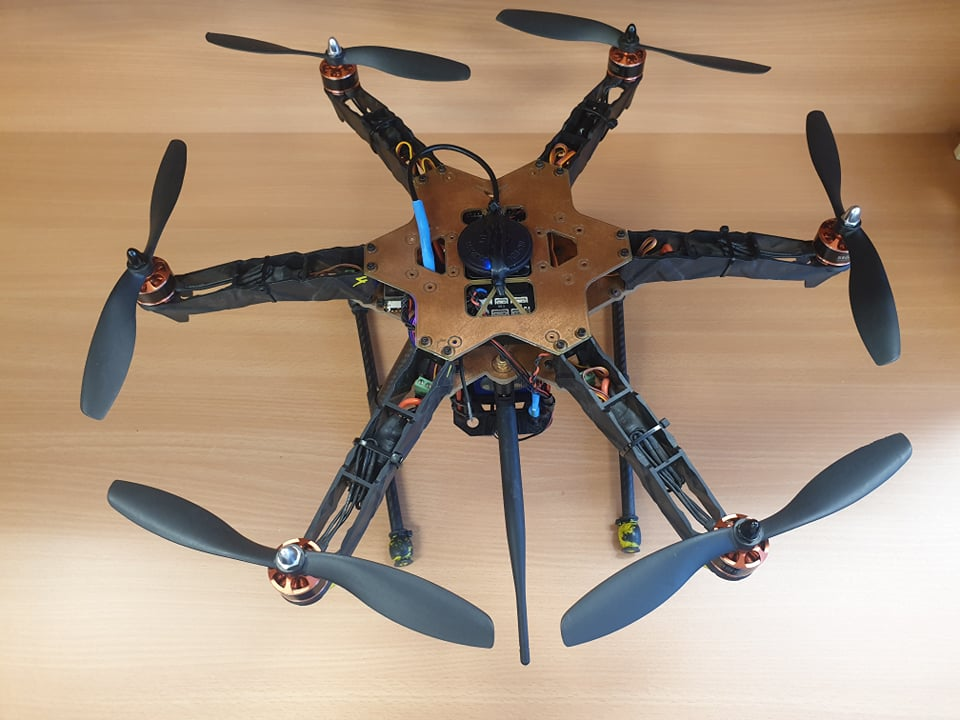
\includegraphics[width=\columnwidth]{Hexacopter_Hardware.jpg}%
	\caption{Hardware platform used for flight testing.}%
	\label{fig:hardware}%
\end{figure}

\subsection{The Cube Autopilot}
The drone is controlled by a commercial flight controller known as The Cube Autopilot (formerly known as Pixhawk 2.1). The Cube runs a 32-bit STM32F427 ARM Cortex M4 core, has 256 kB of RAM and 2 MB of flash. It also has a co-processor (STM32F103), which handles failure conditions. It has a number of connectivity options for peripherals (e.g. UART, I2C, CAN buses), as well as 14 PWM outputs for interfacing with actuators. This platform also has a microSD card slot for storage of flight data logs.
\subsection{ArduPilot Software}
The vehicle is controlled using the open source flight software Ardupilot, with the specific version being ArduCopter 4.1. The flight software is run on a Linux-based real-time operating system (RTOS) known as ChibiOS. The code base is mostly written in C++. State estimation is performed via an EKF-based algorithm. The control system is based on a cascaded PID structure similar to the controller developed in Section \ref{section:PIDControl}. There are also a number of flight modes which are able to be selected for various purposes, i.e. for autonomous flight or radio-controlled flight.

\subsection{Companion Computer}
Additionally, a computer-on-module known as the Intel Edison was added to the Cube flight controller in order to enhance the system capabilities and enable wireless communication. The Edison has a 500 MHz dual-core processor, 1 GB RAM, 4 GB storage and dual-band (2.4 and 5 GHz) WiFi connectivity. The Edison is connected via a designated 70-pin Hirose DF40 connector inside the case of the Cube. Communication with the ArduPilot software is via the MAVLink communication protocol.

APSync, an open source software package developed for use with ArduPilot, was installed on the Edison. This included a Linux operating system as well as a number of python and DroneKit packages. DroneKit is an open source API which allows python scripts to be run on flight control hardware. 

Another feature of the APSync package is the WiFi access point that is created upon start up. This allows wireless connection to the flight controller via the Edison and also allows User Datagram Protocol (UDP) packets to be sent and received. However, it was determined that receiving sensor data via a UDP socket was too slow to effectively estimate states. The Edison is also able to be accessed via Secure Shell (SSH), which allows access to the Linux terminal.



\subsection{Ground Station}
Planning flights and transferring recorded data was accomplished via a ground station software - Mission Planner. The user interface (UI) allows autonomous flights to be planned, initiated and tracked on a map. This software also allows parameters in the ArduPilot software to be viewed and edited. Connection from the ground station to the flight controller can be established via a USB connection, however this means flight data can not be monitored in real time. The Edison allows a UDP connection to be established to both send commands and receive data. An example of a flight plan in the UI is shown in \figref{fig:MissionPlanner}

\begin{figure}[htb]
\begin{center}
	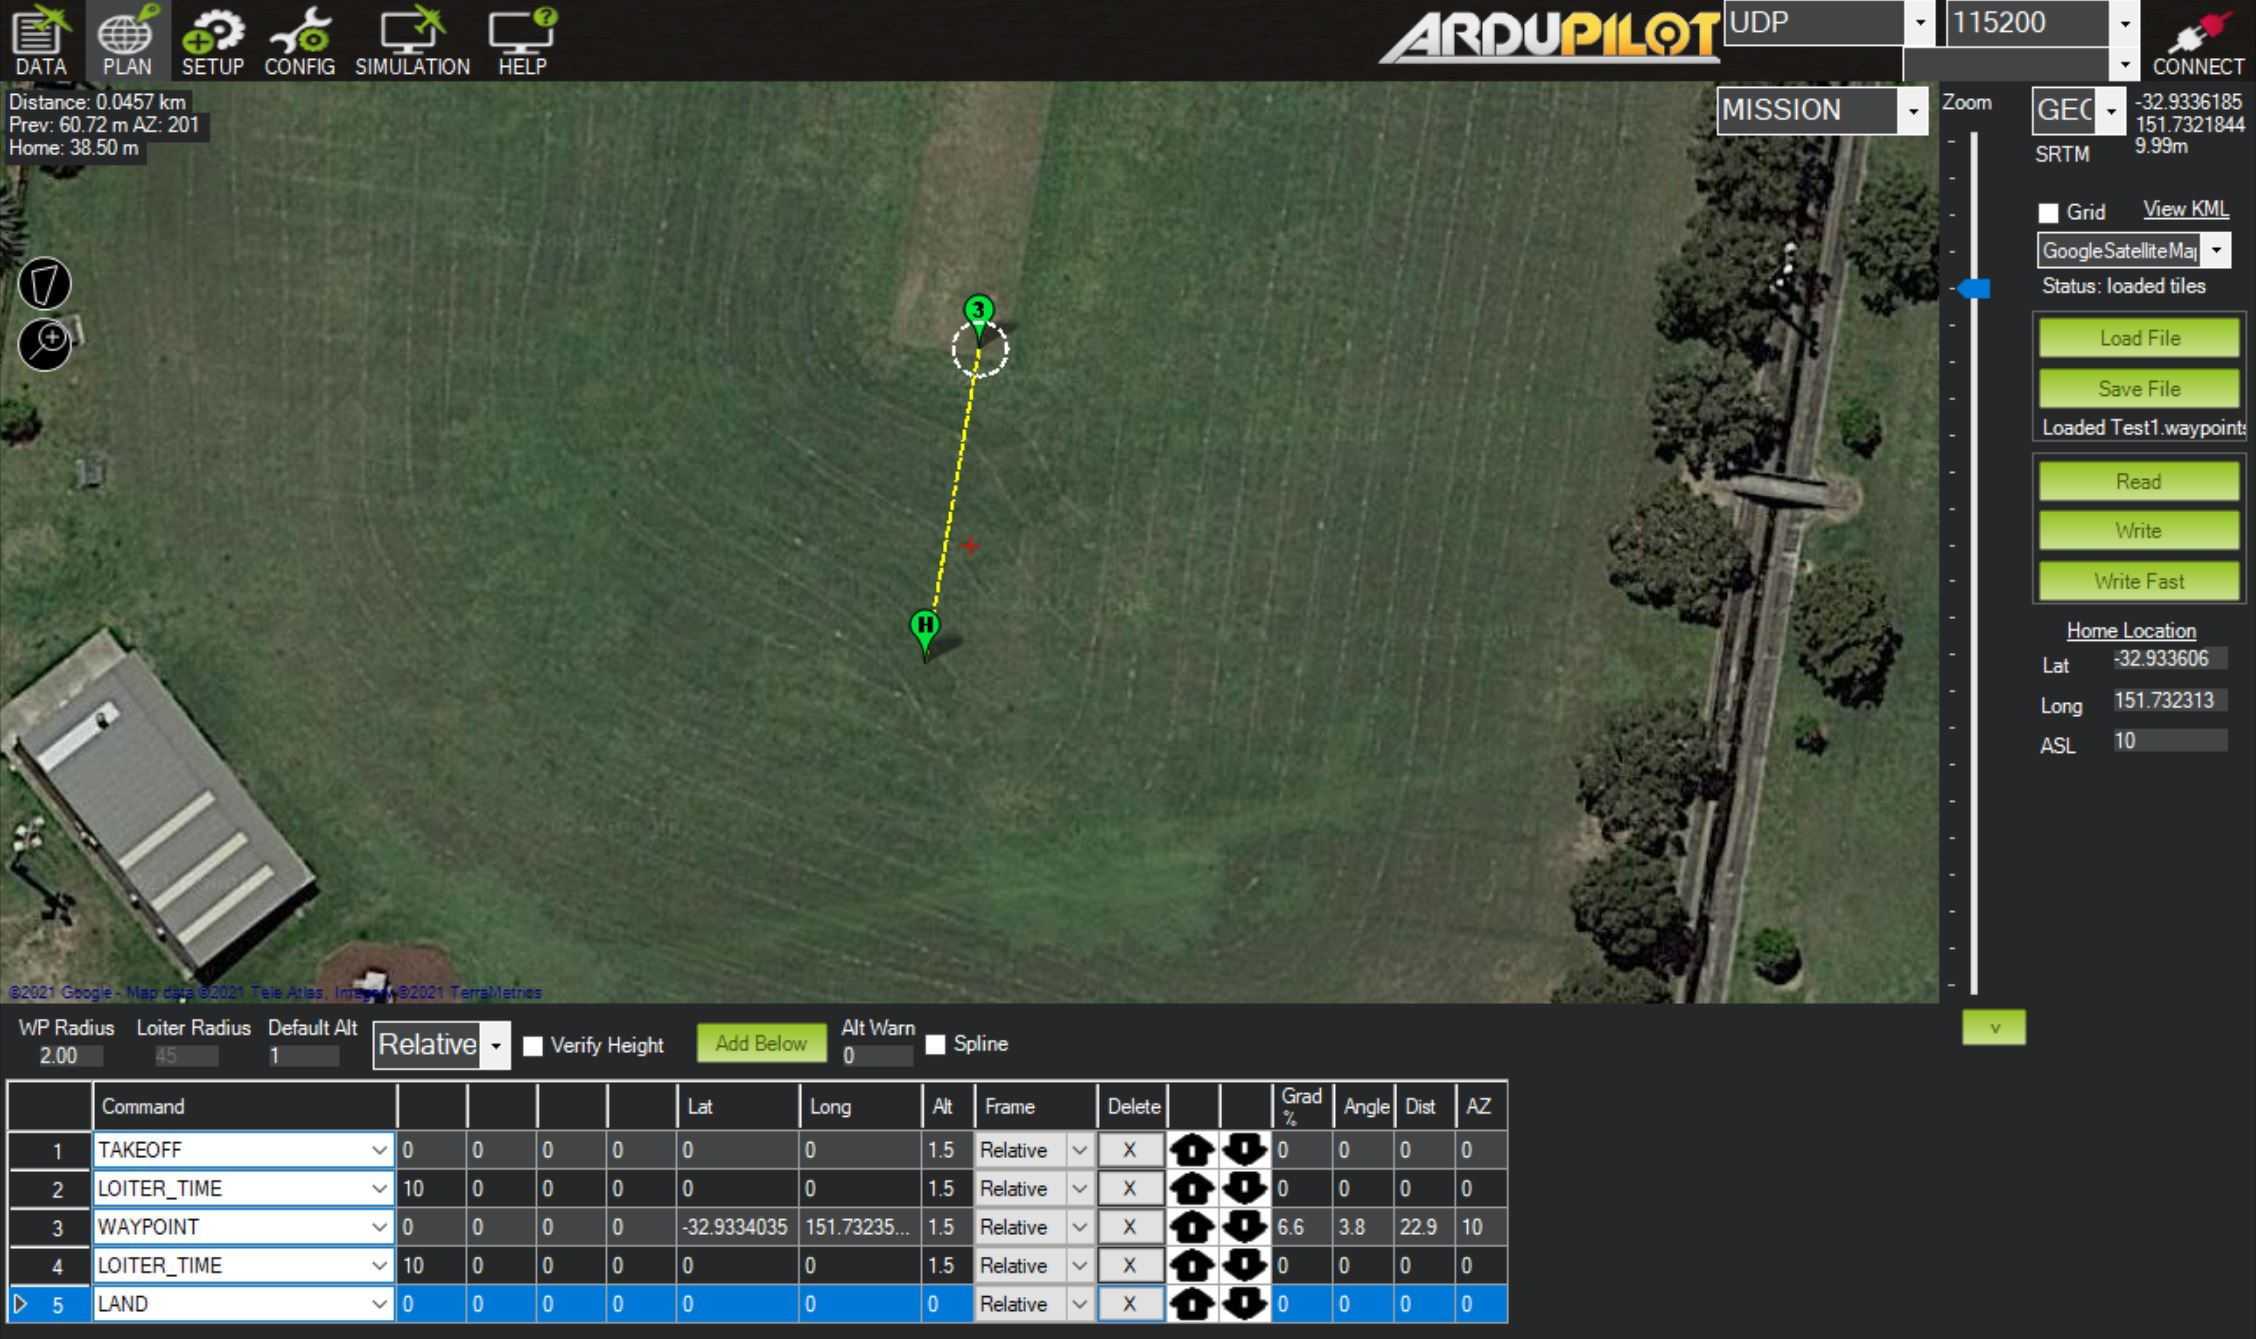
\includegraphics[width=\columnwidth]{MissionPlanner.jpg}%
	\end{center}
	\caption{Example of flight plan in Mission Planner UI.}%	
	\label{fig:MissionPlanner}
\end{figure}
\clearpage
The relationship between the different systems is shown in \figref{fig:ArduArch}. 

\begin{figure}[htb]
\begin{center}
	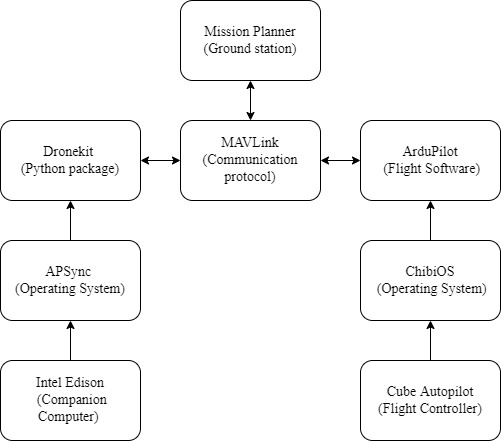
\includegraphics[width=80mm]{ArduPilotArchitecture.jpg}%
	\end{center}
	\caption{System hardware, software and firmware interconnections.}%	
	\label{fig:ArduArch}
\end{figure}

\FloatBarrier
\subsection{Sensors}
The Cube flight controller contains three sets of IMUs (accelerometer, gyroscope and magnetometer), two of which are mechanically vibration-isolated. Two of the IMUs are the Invensense MPU9250 and the third is made up of the STM LSM303D (accelerometer and magnetometer) and L3GD20 (gyroscope). The Cube also contains two barometers, both of which are the MS5611. Multiple of each sensor are provided for redundancy and the EKF in the ArduPilot firmware fuses the data from all sensors for additional accuracy.

Additional sensors were connected to the Cube Autopilot system to enable the previously developed EKFs to be tested.  

A Ublox NEO-M8N GPS module was connected to provide positional data. This module also houses a magnetometer for additional external measurement of the Earth's magnetic field. The GPS module communicates with the flight controller via the I2C protocol.


An integrated optical flow and lidar sensor, Matek 3901-L0X, was also connected to the system. This module consists of a Pimoroni PMW3901 optical flow sensor, an Adafruit VL53L0X lidar sensor and a STM32L051 microcontroller, as well as additional power regulating circuitry. This sensor is able to communicate over UART using Multiwii Serial Protocol (MSP), which is supported by the ArduPilot firmware.


\FloatBarrier
\section{Flight Testing}
Flight testing was conducted by programming the hexacopter with an autonomous mission via the ground station. The first test flight  which involved taking off to a height of 1.5 metres, travelling approximately 11 metres to a second position and landing. The drone performed the mission successfully using the ArduPilot flight control software and the sensor data recorded during the flight was logged to the onboard SD card. For this flight test, the OFS had not yet been configured and the GPS was used for positional data. This data was processed in MATLAB and used with the GPS EKF algorithm described in Section \ref{section:GPS_EKF}. \figref{fig:HW_GPS_Pos} shows the position and velocity results, and \figref{fig:HW_GPS_Ang} shows the angular results. The estimates produced by the previously developed algorithm are compared with the estimates of the ArduPilot (AP) software. Note that for the yaw angle results, an angle of $2\pi$ radians is equivalent to 0 radians, which explains the sudden decline in these results. The estimated yaw angle climbs above $2\pi$ radians before correcting and returning towards zero in the correct range. 

\begin{figure}[htb]
	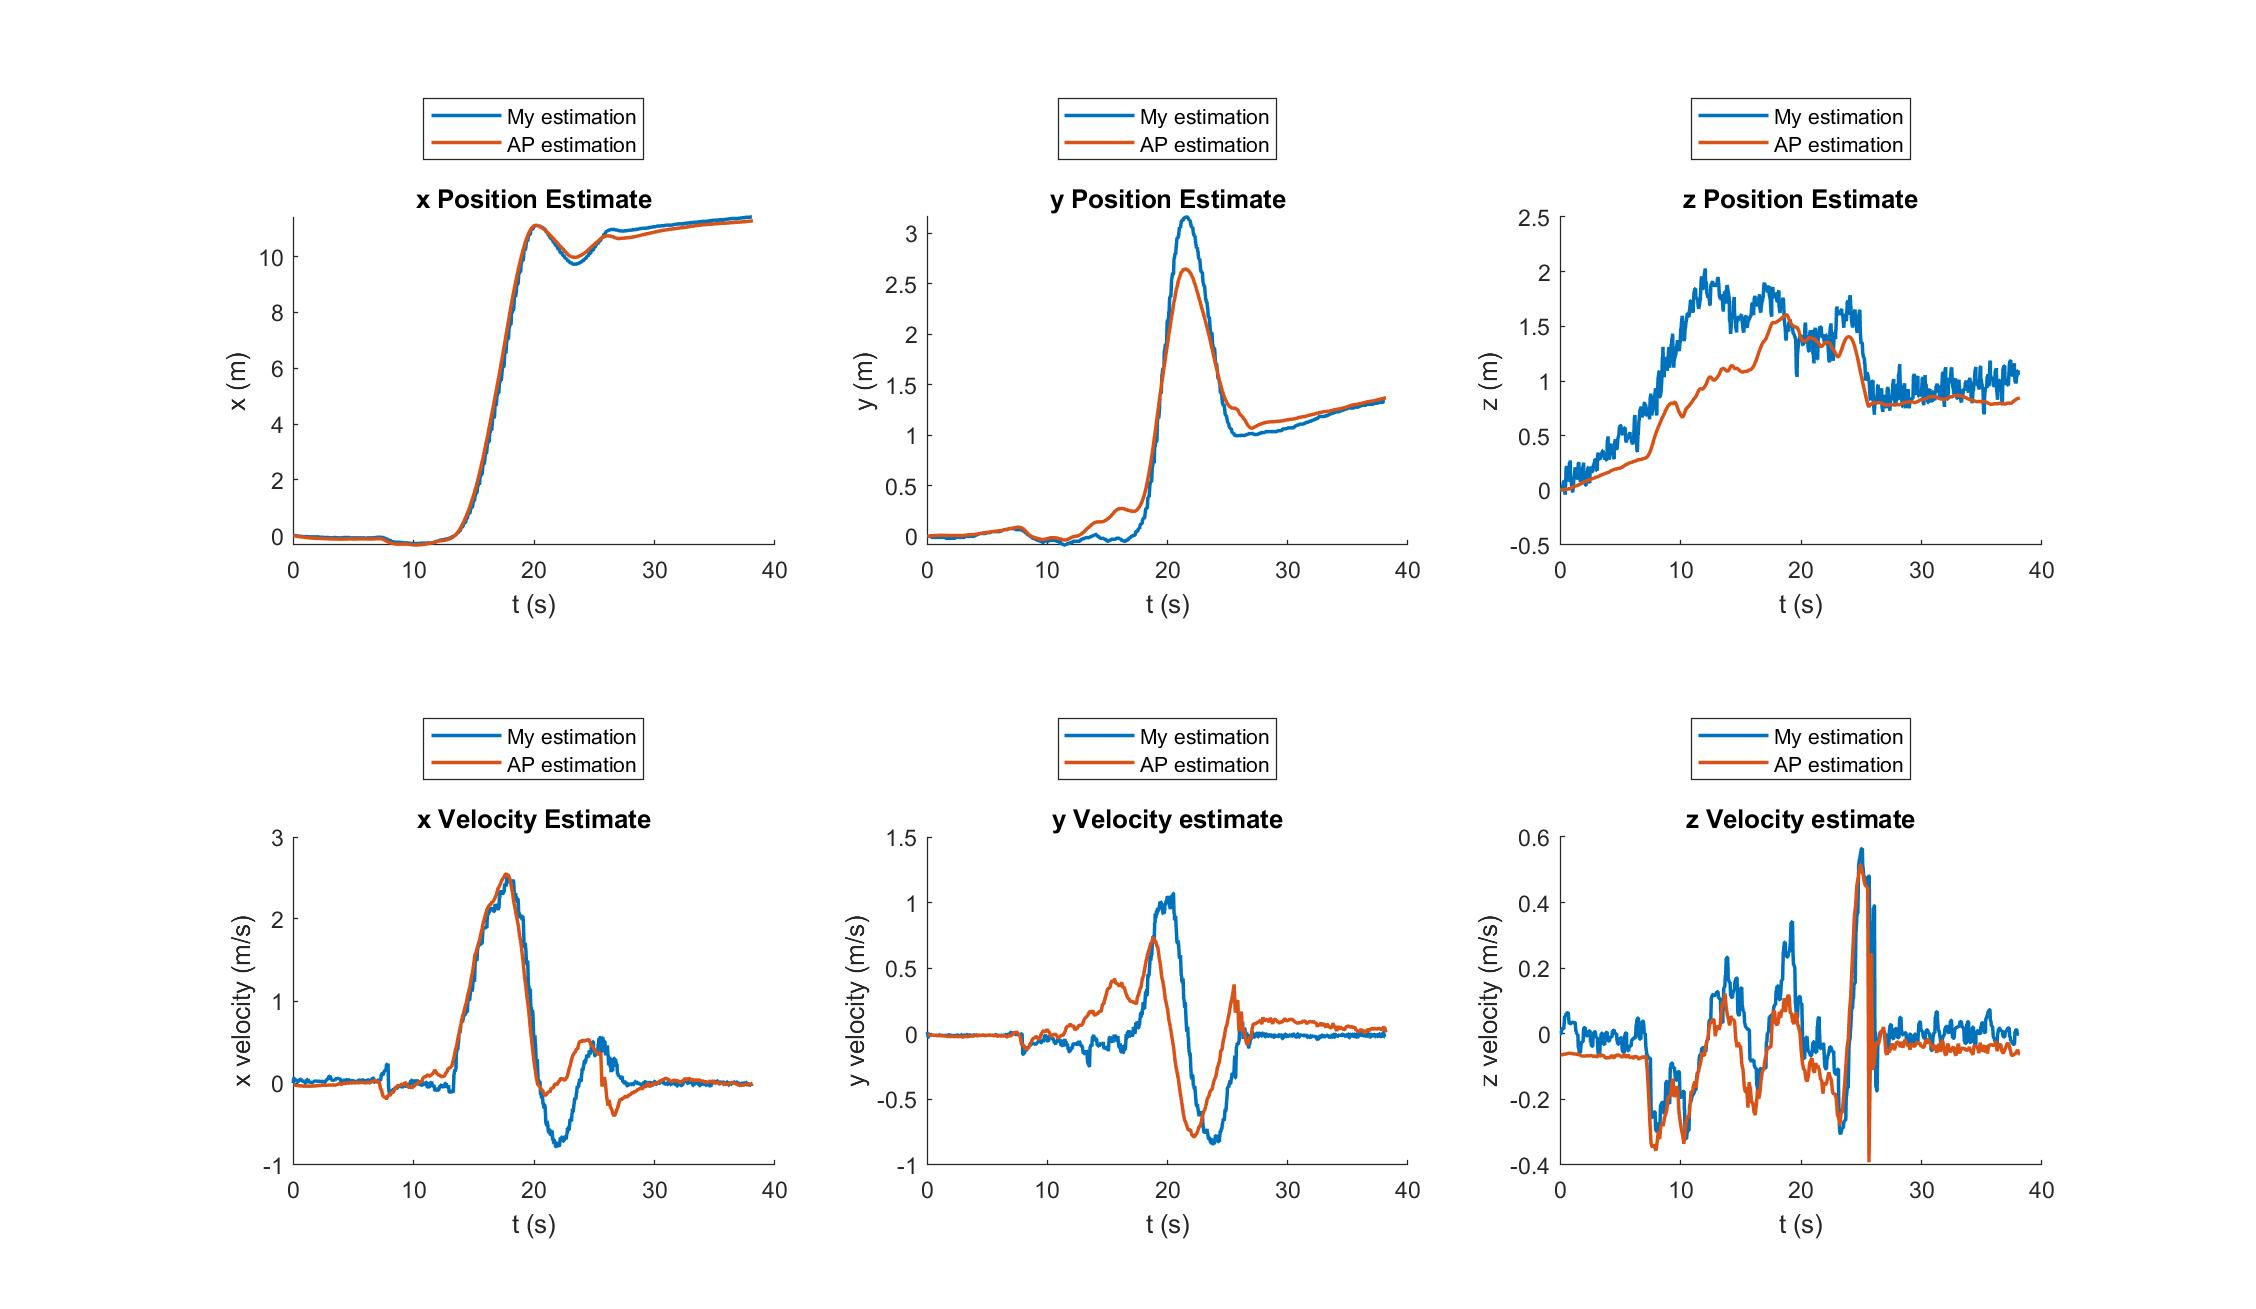
\includegraphics[width=\columnwidth]{EKF_HW/GPS/FlightTest1_Pos.jpg}%
	\caption{The GPS EKF position and velocity estimates compared with the ArduPilot EKF estimates for flight test \#1.}%
	\label{fig:HW_GPS_Pos}%
\end{figure}

\begin{figure}[htb]
	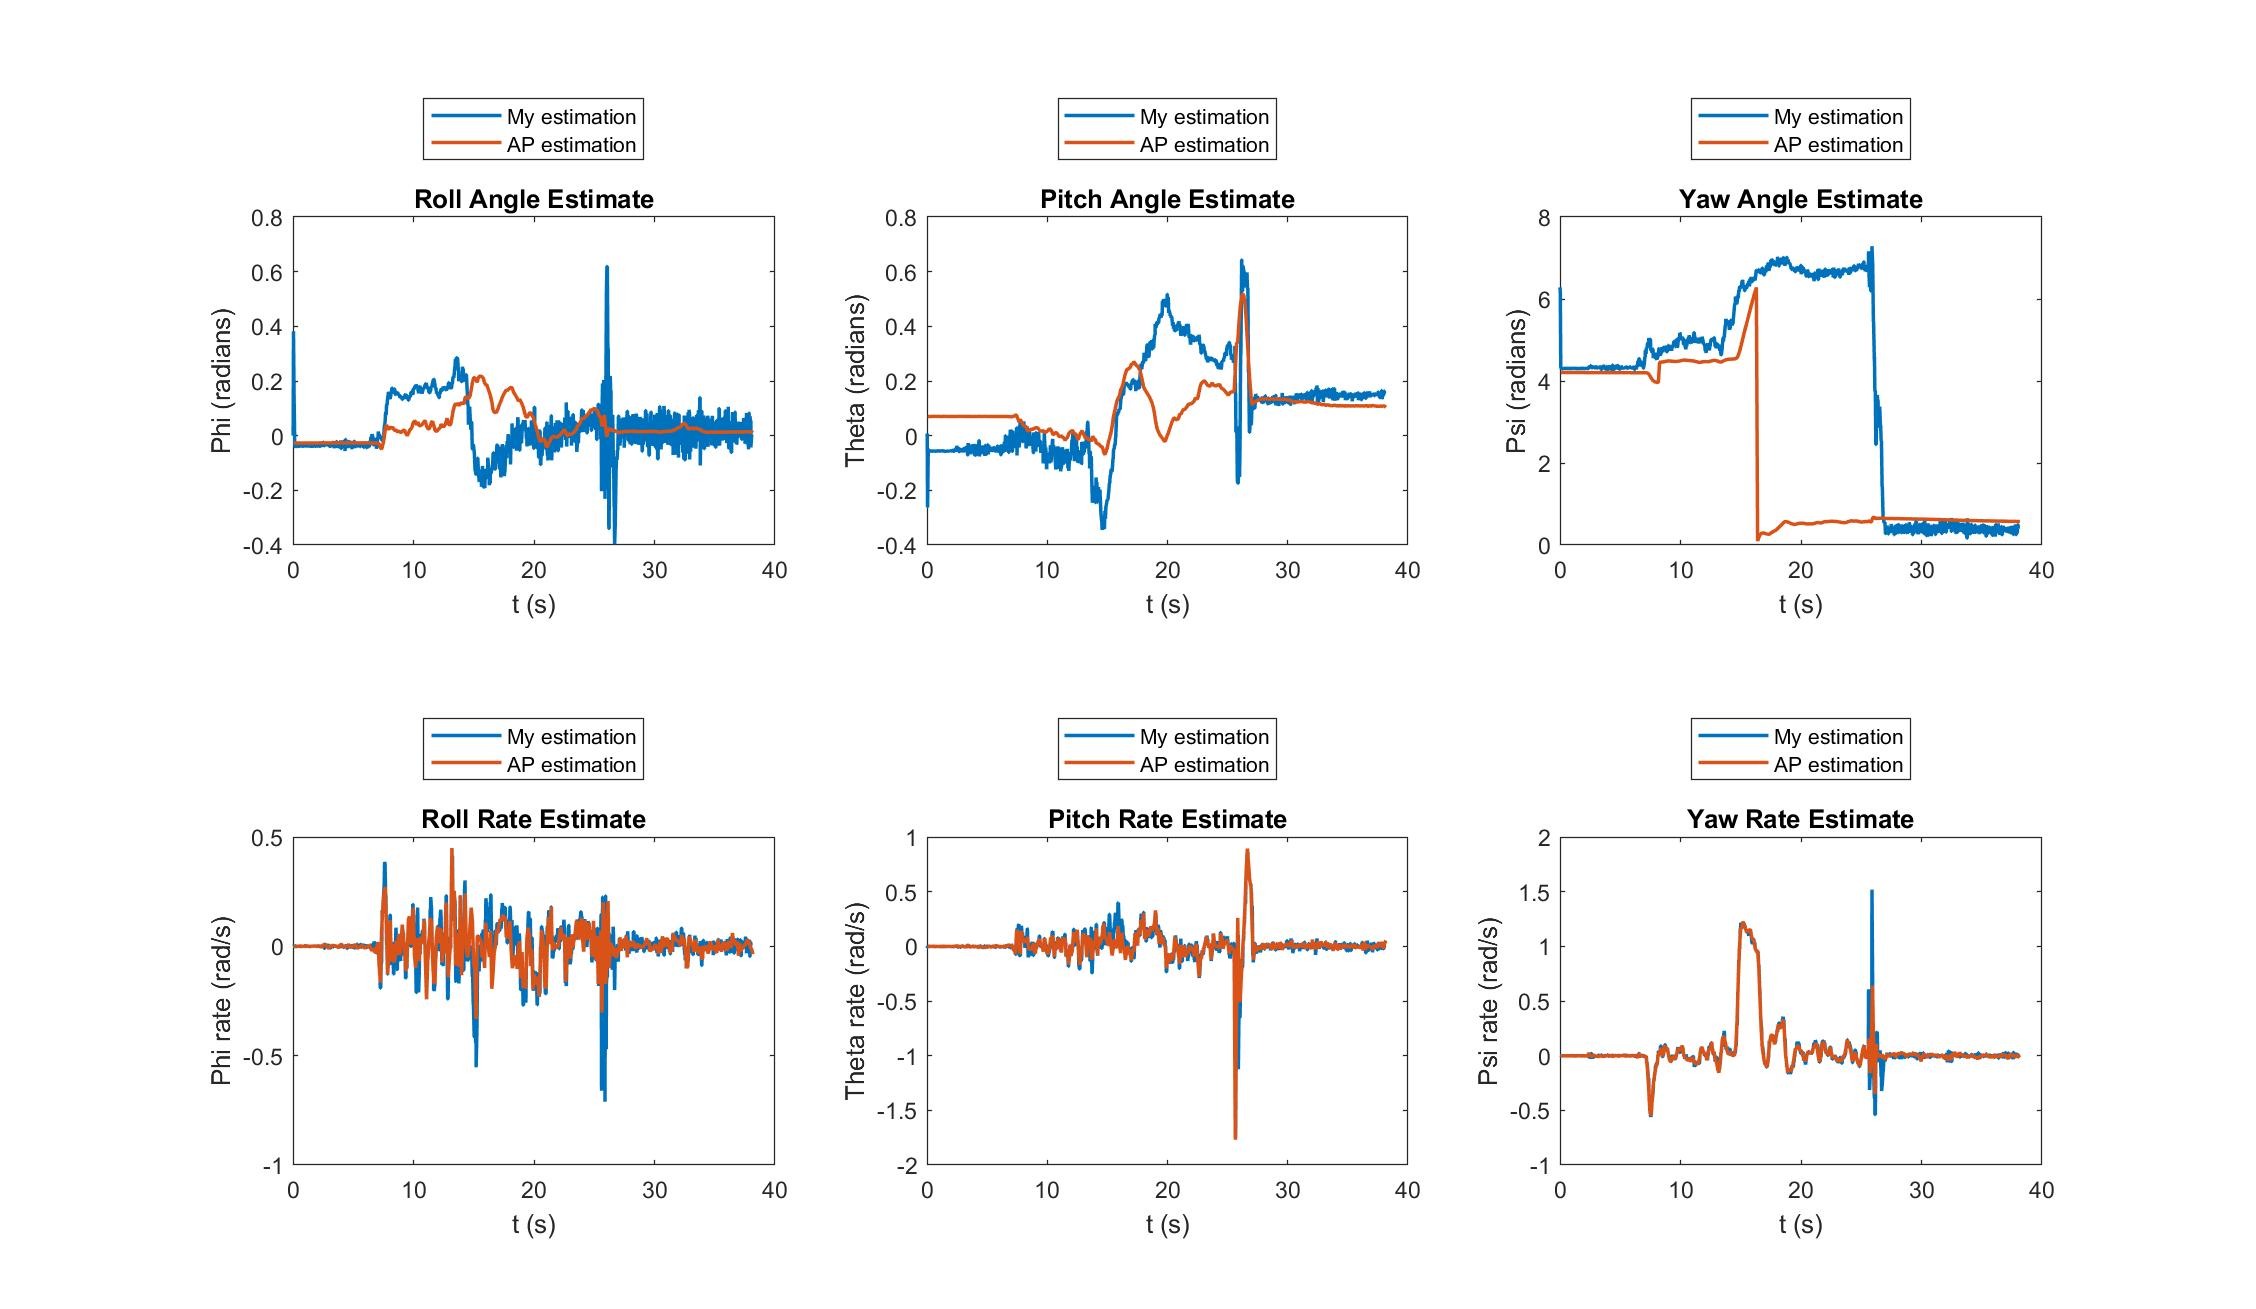
\includegraphics[width=\columnwidth]{EKF_HW/GPS/FlightTest1_Angle.jpg}%
	\caption{The EKF angular estimates compared with the ArduPilot EKF estimates for flight test \#1.}%
	\label{fig:HW_GPS_Ang}%
\end{figure}

A flight test was then repeated with the optical flow sensor installed to evaluate the effectiveness of the EKF in the absence of GPS data. This flight involved taking off to a height off approximately 1.5 m, hovering at that point for approximately 10 seconds and then landing at the same point. The results of the EKF are shown in \figref{fig:HW_OFS_Pos}, compared with the AP estimation (which uses GPS data). The position and velocity estimates are not extremely accurate, however it can be seen that there is no significant drift in the position estimates over this time period.

\begin{figure}[htb]
	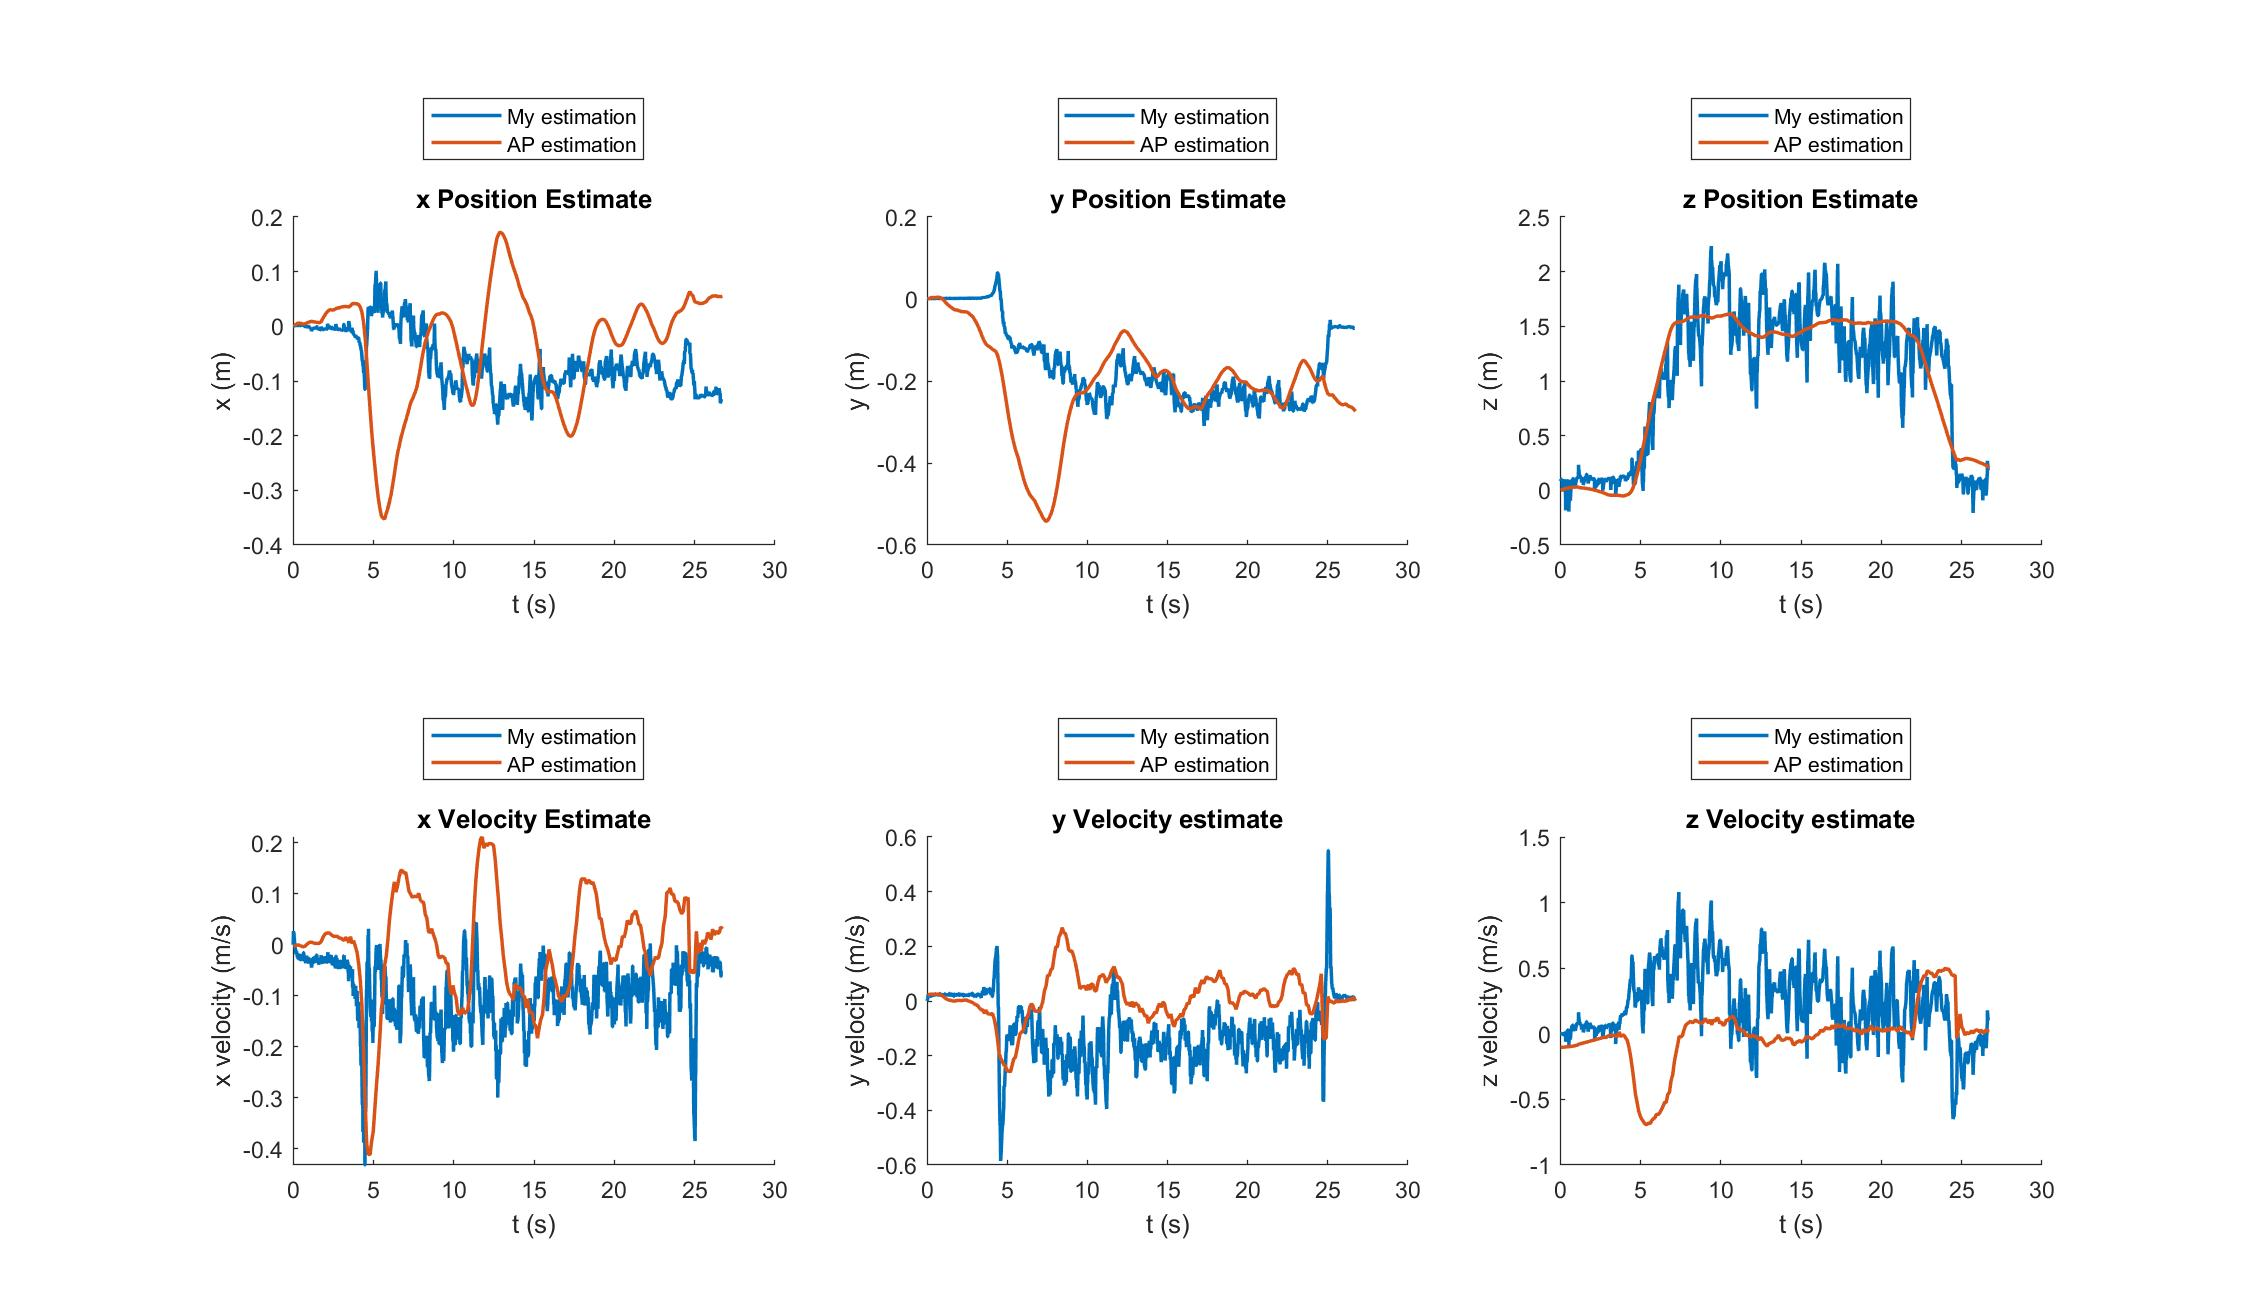
\includegraphics[width=\columnwidth]{EKF_HW/OFS/FlightTest2_Pos.jpg}%
	\caption{The OFS EKF position and velocity estimates compared with the ArduPilot EKF estimates for flight test \#2.}%
	\label{fig:HW_OFS_Pos}%
\end{figure}

A third flight was undertaken in which the aircraft was programmed to take off to 1.5m, hover in place for 10 seconds, then travel some distance to land at another waypoint. This flight resulted in a collision with the ground- likely due to unreliable lidar data. However the first 25 seconds of data was able to be used for analysis. Using this data, it could be seen that using the OFS data alone was insufficient for tracking positional change. The y velocity estimate did not show any significant motion despite the vehicle travelling approximately 12 metres within four seconds. These results are shown in \figref{fig:HW_OFS_Pos_2}.

\begin{figure}[htb]
	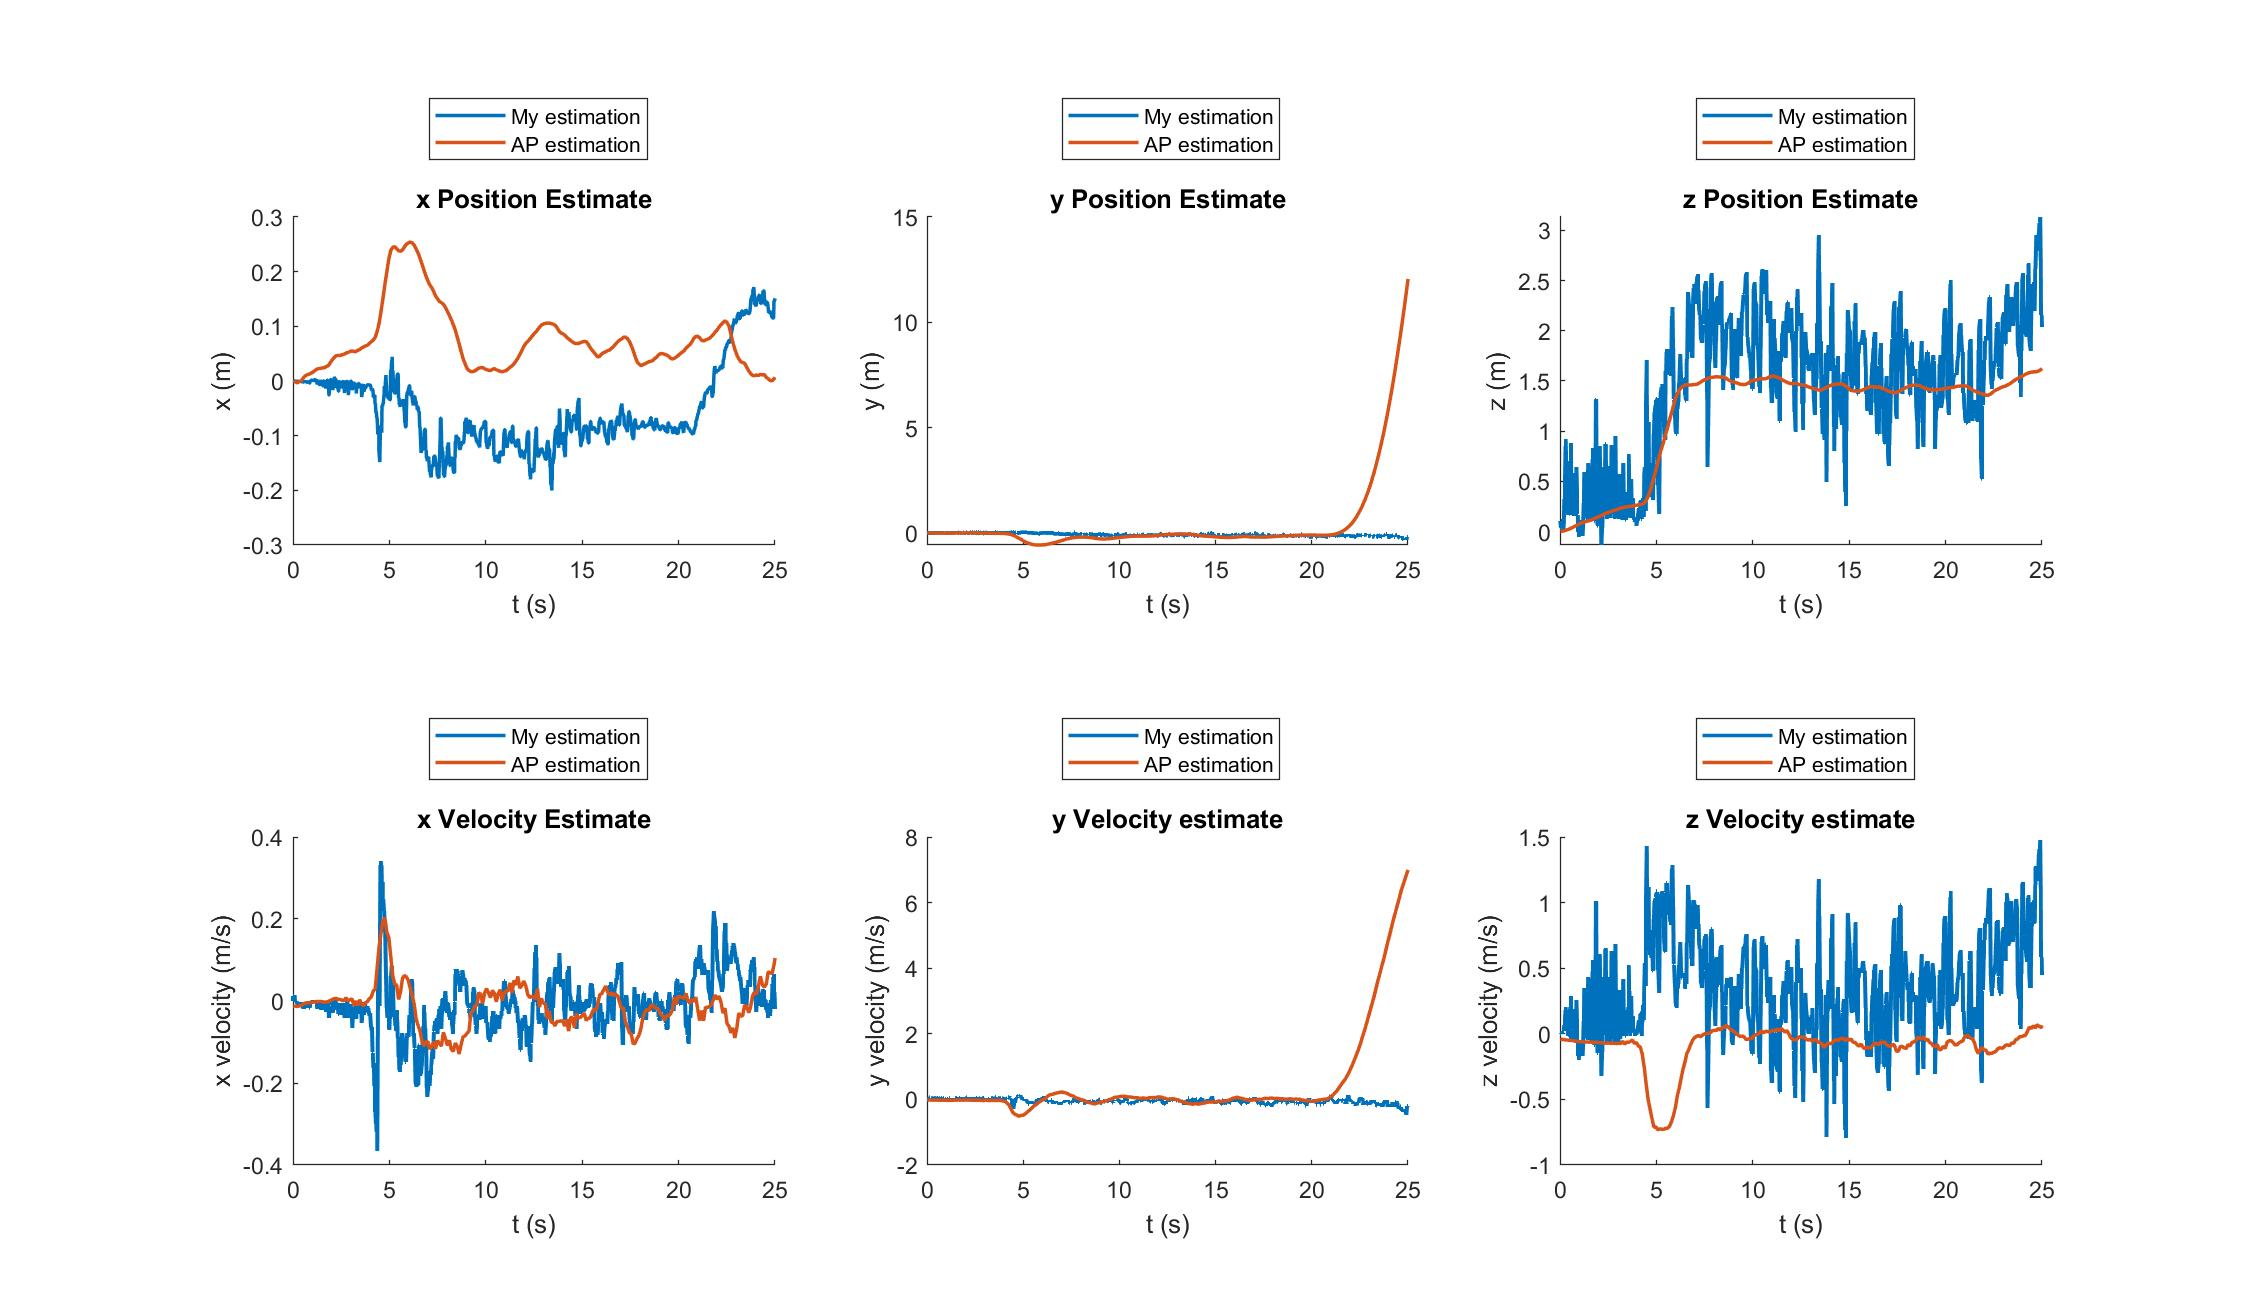
\includegraphics[width=\columnwidth]{EKF_HW/OFS/Flight_Test3_Pos.jpg}%
	\caption{The OFS EKF position and velocity estimates compared with the ArduPilot EKF estimates for flight test \#3.}%
	\label{fig:HW_OFS_Pos_2}%
\end{figure}

\FloatBarrier
\section{Discussion of Results}
To produce these results, the sensor data that was recorded on the SD card was processed post-flight in MATLAB. It is important to note that the data which is recorded on the SD card is not representative of all the sensor data available to the flight controller. That is, the flight controller samples the sensors at a faster rate and not all data is logged. This severely limits the accuracy of the estimated states which are based upon this data. For example, the IMU is sampled at a rate of at least 1 kHz, however the data is logged at a rate of approximately 25 Hz. This issue was particularly prominent for the optical flow sensor data, which was logged at a rate of only 10 Hz but has a capability of 121 Hz. If the EKF was run directly on the hardware it may prove to be more accurate. \\

Another issue that arose was the unreliability of the lidar data. The datasheet states that the sensor only has an operating range of 2 m. Although, the flight test was conducted at 1.5 m above the ground, the angle of the vehicle during translational motion presumably caused the lidar line-of-sight distance to ground to exceed 2 m. This resulted in the lidar being unable to record data and therefore impacting the accuracy of the results - since the optical flow velocity estimates rely on knowledge of the scene depth. The operating range of this sensor makes it essentially useless for practical flights. However there are many other commercially available lidar sensors with larger operating ranges. Alternatively, many optical flow sensors are instead paired with sonar (ultrasonic) sensors for scene depth information.\\

It is also worth noting that sensors generally have significant biases and there are a number of models to describe the behaviour of sensor bias. A common model used in Kalman filter techniques is the random-walk model \cite{Sabatini2011}. Errors were likely introduced into the data due to this effect and the developed algorithms do not account for this.



\section{Chapter Summary}
This chapter introduced the hexacopter platform's hardware and software architecture. A number of flight tests were carried out and the data was processed post-flight using the previously developed EKF algorithms. It is shown that with the particular optical flow sensor that was chosen, position data was not able to be accurately estimated during motion.

\clearpage




\chapter{Conclusion and Extensions}

\section{Conclusion}

\section{Future Extensions}
There are many possible extensions to this project, for example:

\begin{itemize}
\item Implement the backstepping control system on the hardware platform.\\
\item Account for motor/propeller failure events during flight.\\
\item Extend sensor fusion algorithm to handle sensor failure.\\
\item Implement obstacle avoidance.\\
\item Analyse the usefulness of additional sensors.\\
\item Consider the impacts of other effects e.g air resistance and gyroscopic effects.\\
\item Consider slew rates of actuators, propeller inertia, etc.\\
\item Use quaternions to avoid singularities.


\end{itemize}

\clearpage







%%%%%%%%%%%%%%%%%%%%%%%%%%%%%%%%%%%%%%%%%%%%%%%%%%%%%%%%%%%%%
%% BIBLIOGRAPHY AND OTHER LISTS
%%%%%%%%%%%%%%%%%%%%%%%%%%%%%%%%%%%%%%%%%%%%%%%%%%%%%%%%%%%%%
%% A small distance to the other stuff in the table of contents (toc)
\addtocontents{toc}{\protect\vspace*{\baselineskip}}



%%%%%%%%%%%%%%%%%%%%%%%%%%%%%%%%%%%%%%%%%%%%%%%%%%%%
%%%%%%%%%        BIBLIOGRAPHY        %%%%%%%%%%%%%%%
%%%%%%%%%%%%%%%%%%%%%%%%%%%%%%%%%%%%%%%%%%%%%%%%%%%%%
\addcontentsline{toc}{chapter}{Bibliography}%'Bibliography' into toc
%\nocite{*} %Even non-cited BibTeX-Entries will be shown.
\bibliographystyle{ieeetran}
\bibliography{References}

 




%% The List of Figures
%\clearpage
%\addcontentsline{toc}{chapter}{List of Figures}
%\listoffigures

%% The List of Tables
%\clearpage
%\addcontentsline{toc}{chapter}{List of Tables}
%\listoftables


%%%%%%%%%%%%%%%%%%%%%%%%%%%%%%%%%%%%%%%%%%%%%%%%%%%%%%%%%%%%%
%% APPENDICES
%%%%%%%%%%%%%%%%%%%%%%%%%%%%%%%%%%%%%%%%%%%%%%%%%%%%%%%%%%%%%

\begin{appendices}

\pagenumbering{arabic}% resets `page` counter to 1
\renewcommand*{\thepage}{A-\arabic{page}}

\chapter{Simulink Models}\label{appendix:Simulink}

\section{Plant Model}\label{section:Simu_Plant}
\begin{figure}[htb]
\begin{center}
	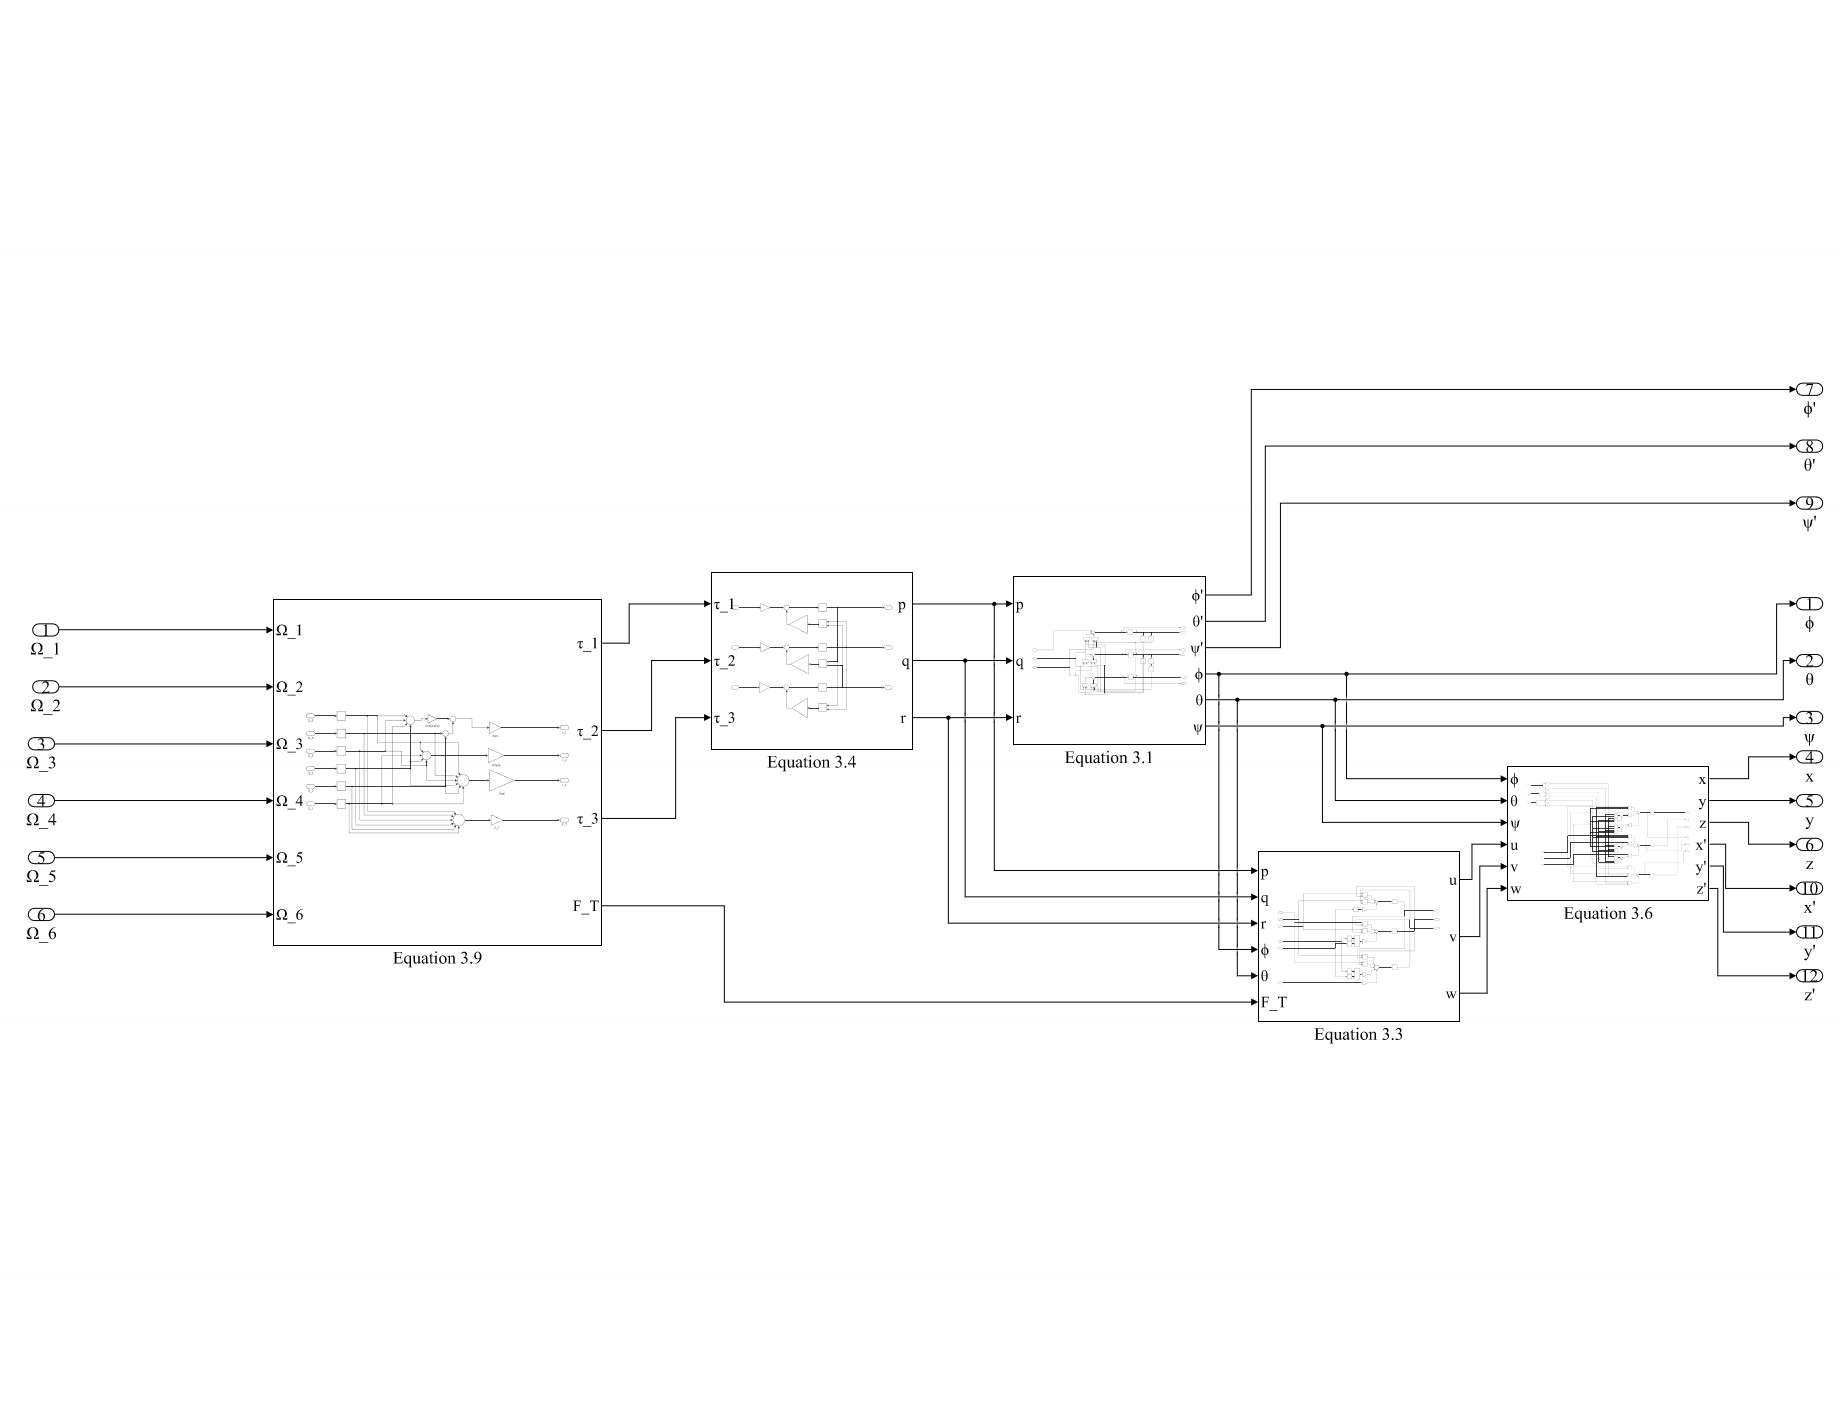
\includegraphics[width=\columnwidth]{/SimulinkModels/Plant/Plant.jpg}%
	\end{center}
	\caption{Hexacopter plant Simulink model overview.}%
\end{figure}

\begin{figure}[htb]
\begin{center}
	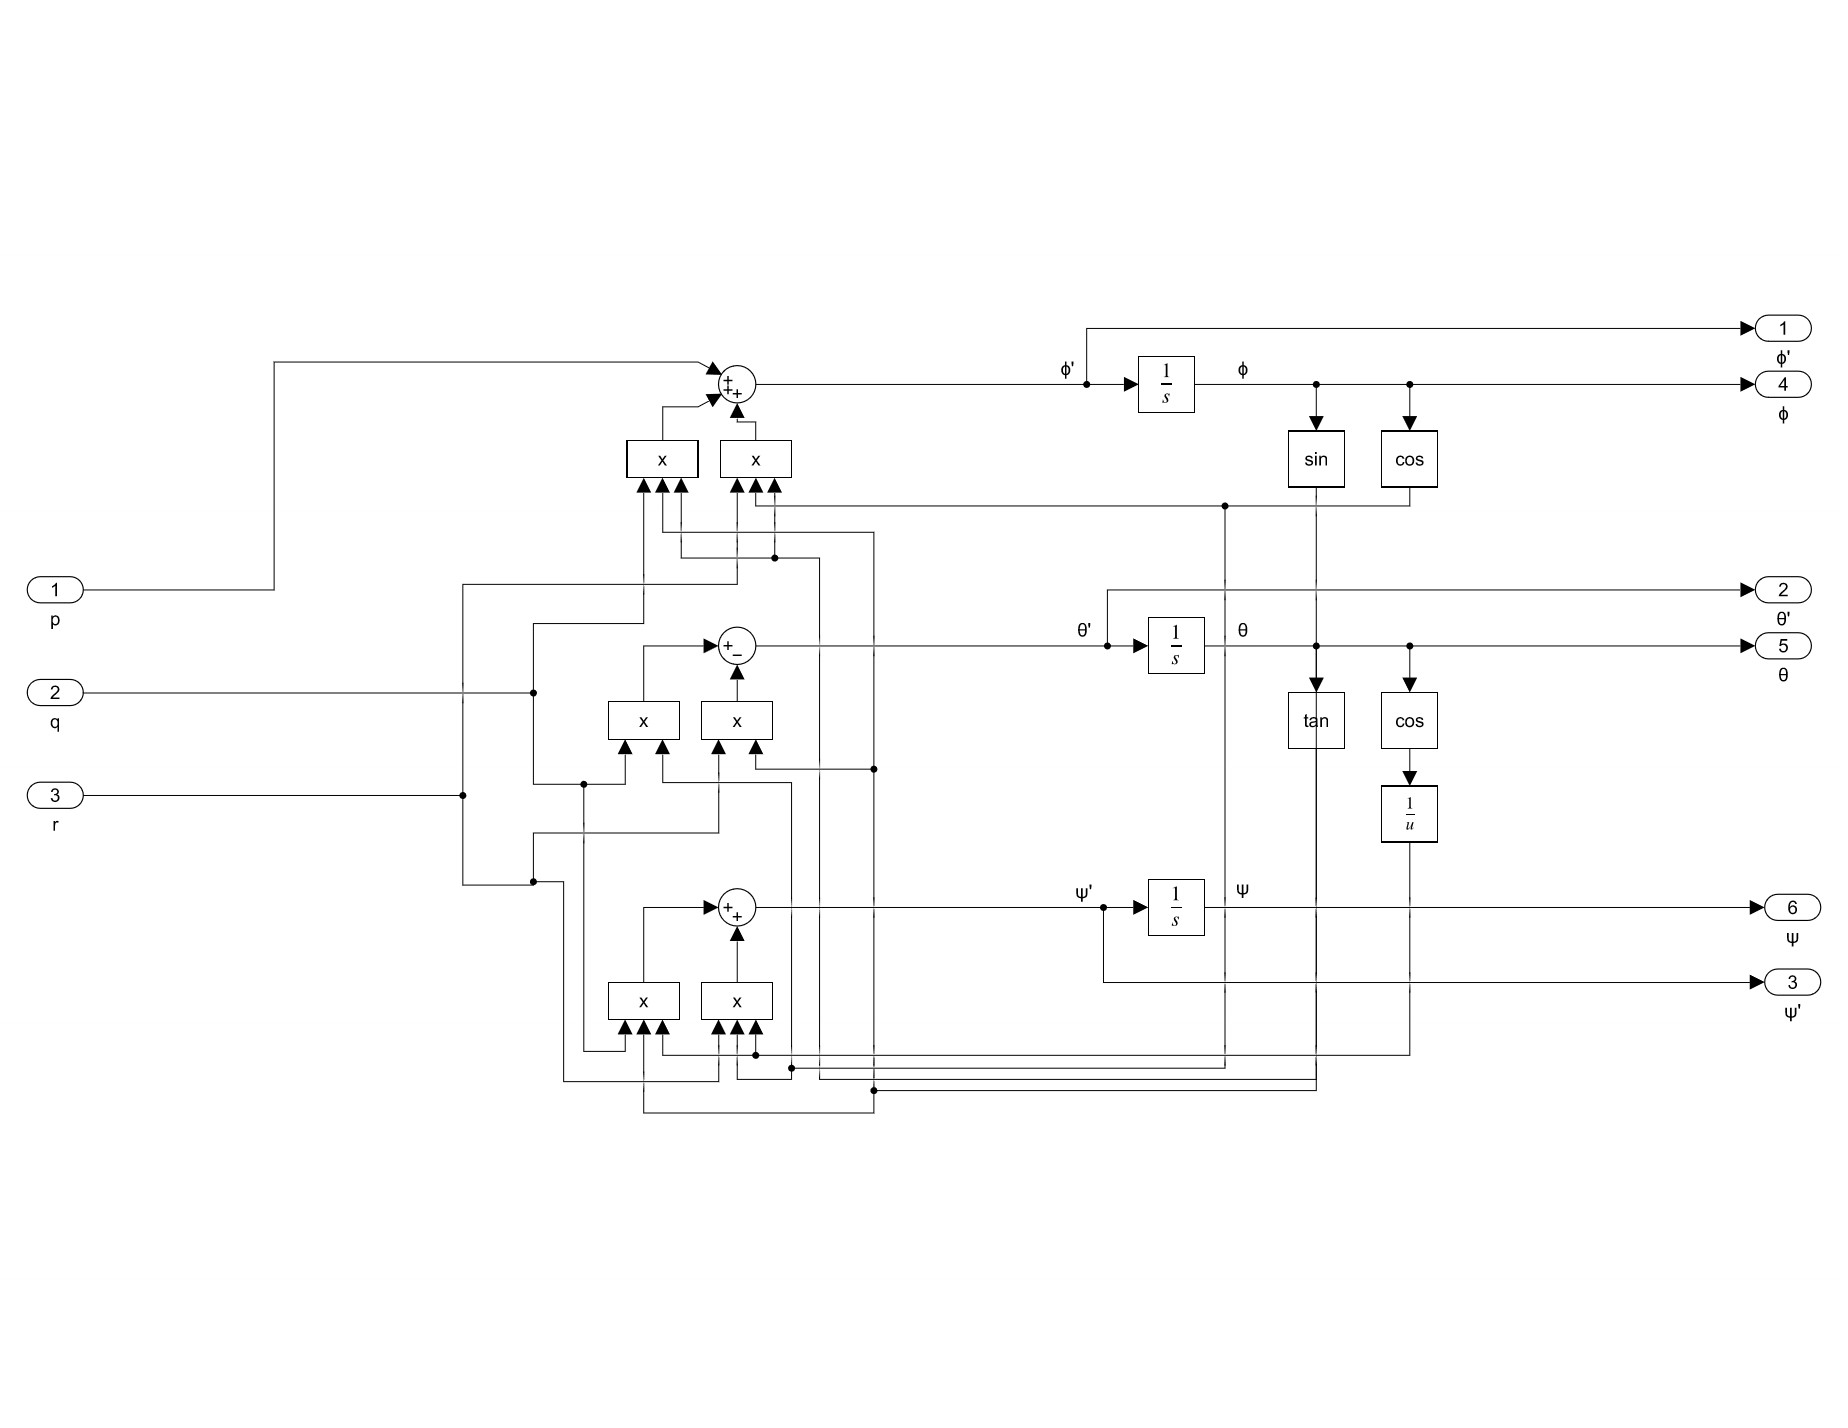
\includegraphics[width=\columnwidth]{/SimulinkModels/Plant/Eq3.1.jpg}%
	\end{center}
	\caption{Equation 3.1 Simulink subsystem.}%
\end{figure}

\begin{figure}[htb]
\begin{center}
	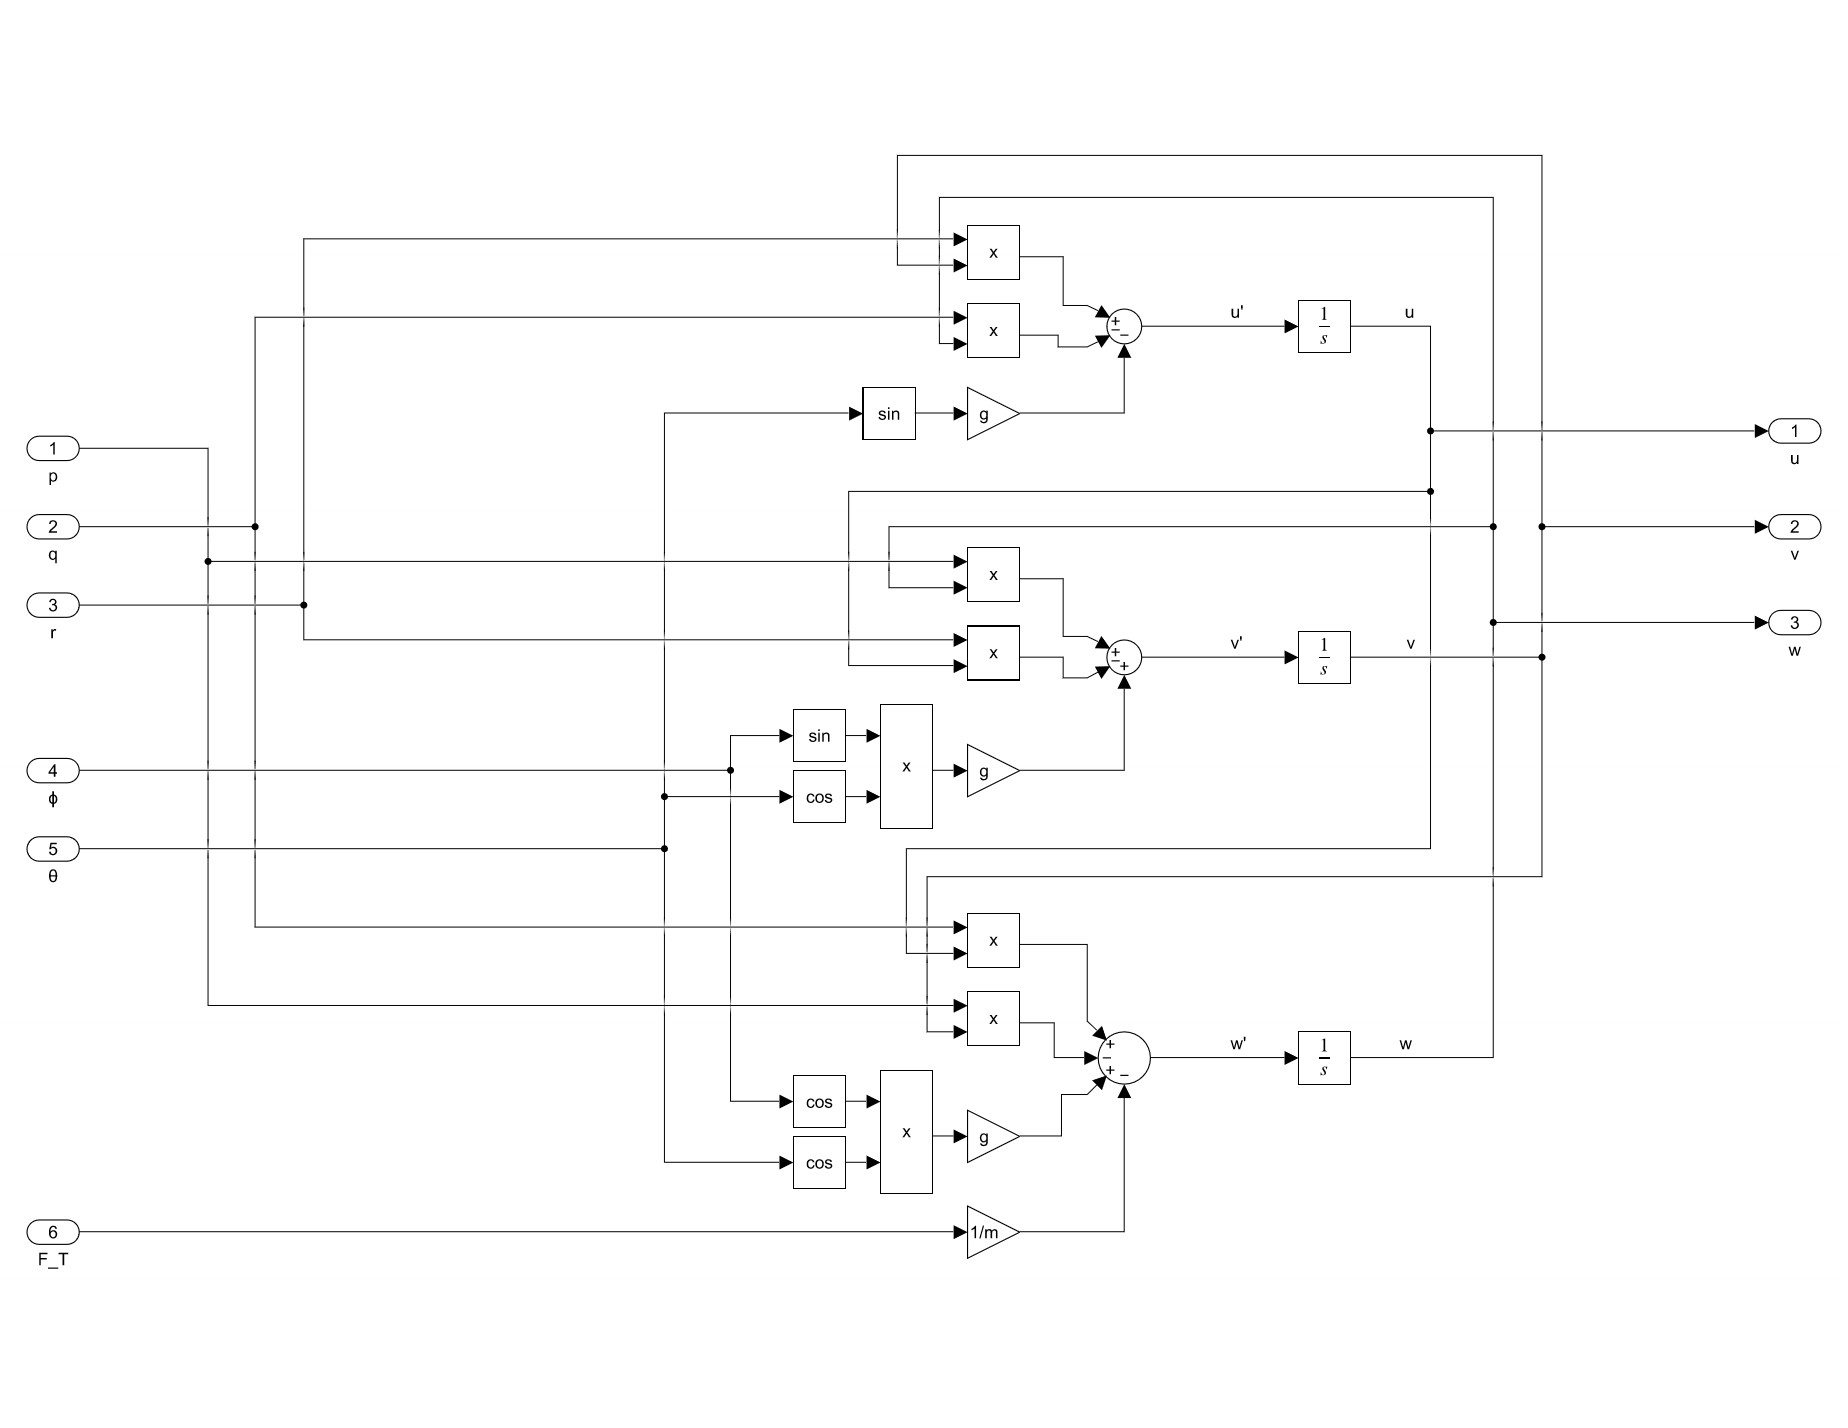
\includegraphics[width=\columnwidth]{/SimulinkModels/Plant/Eq3.3.jpg}%
	\end{center}
	\caption{Equation 3.3 Simulink subsystem.}%
\end{figure}

\begin{figure}[htb]
\begin{center}
	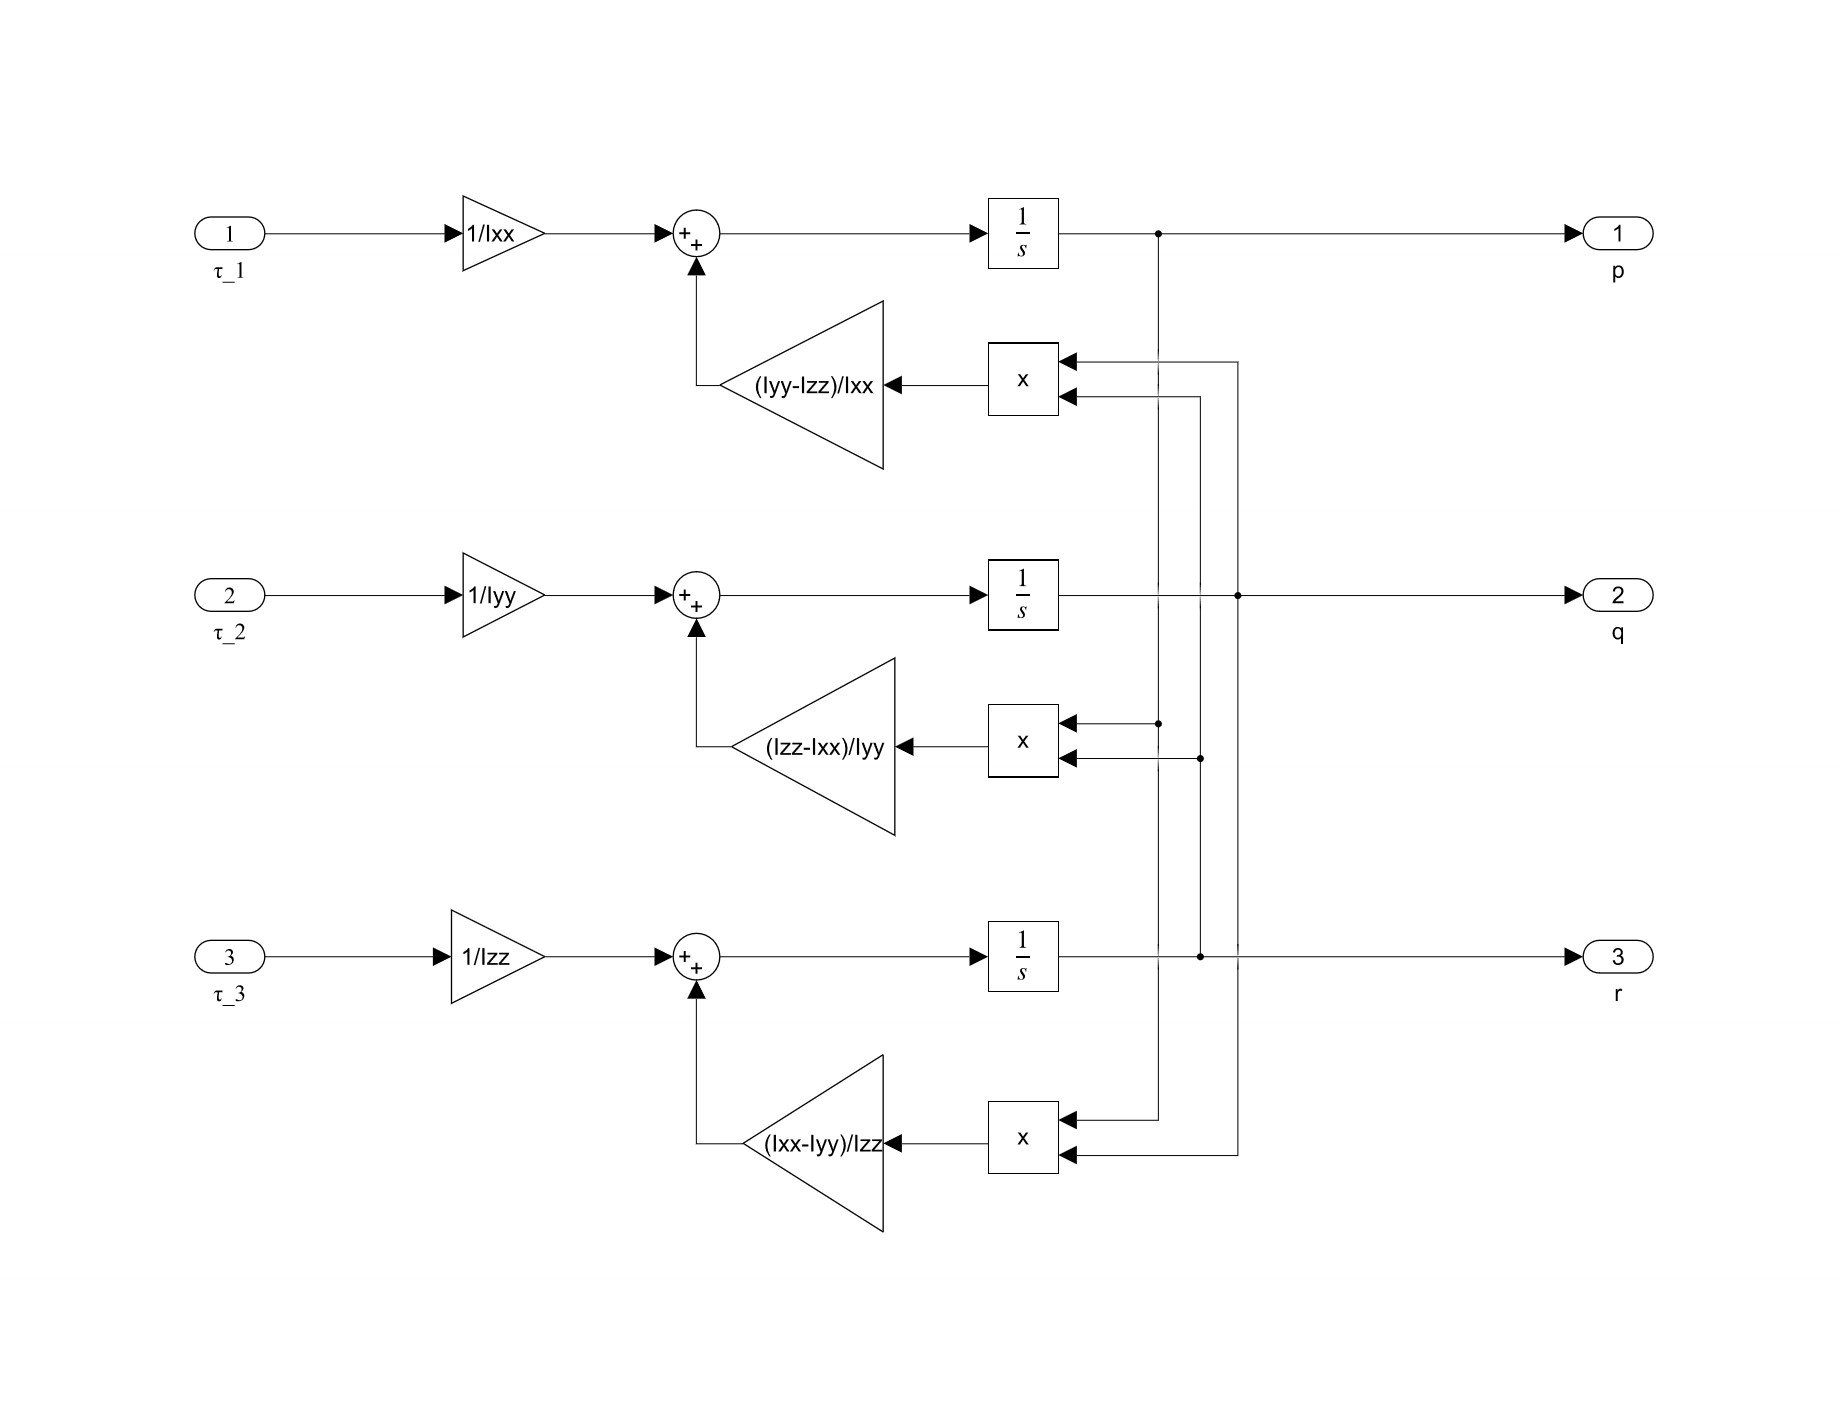
\includegraphics[width=\columnwidth]{/SimulinkModels/Plant/Eq3.4.jpg}%
	\end{center}
	\caption{Equation 3.4 Simulink subsystem.}%
\end{figure}

\begin{figure}[htb]
\begin{center}
	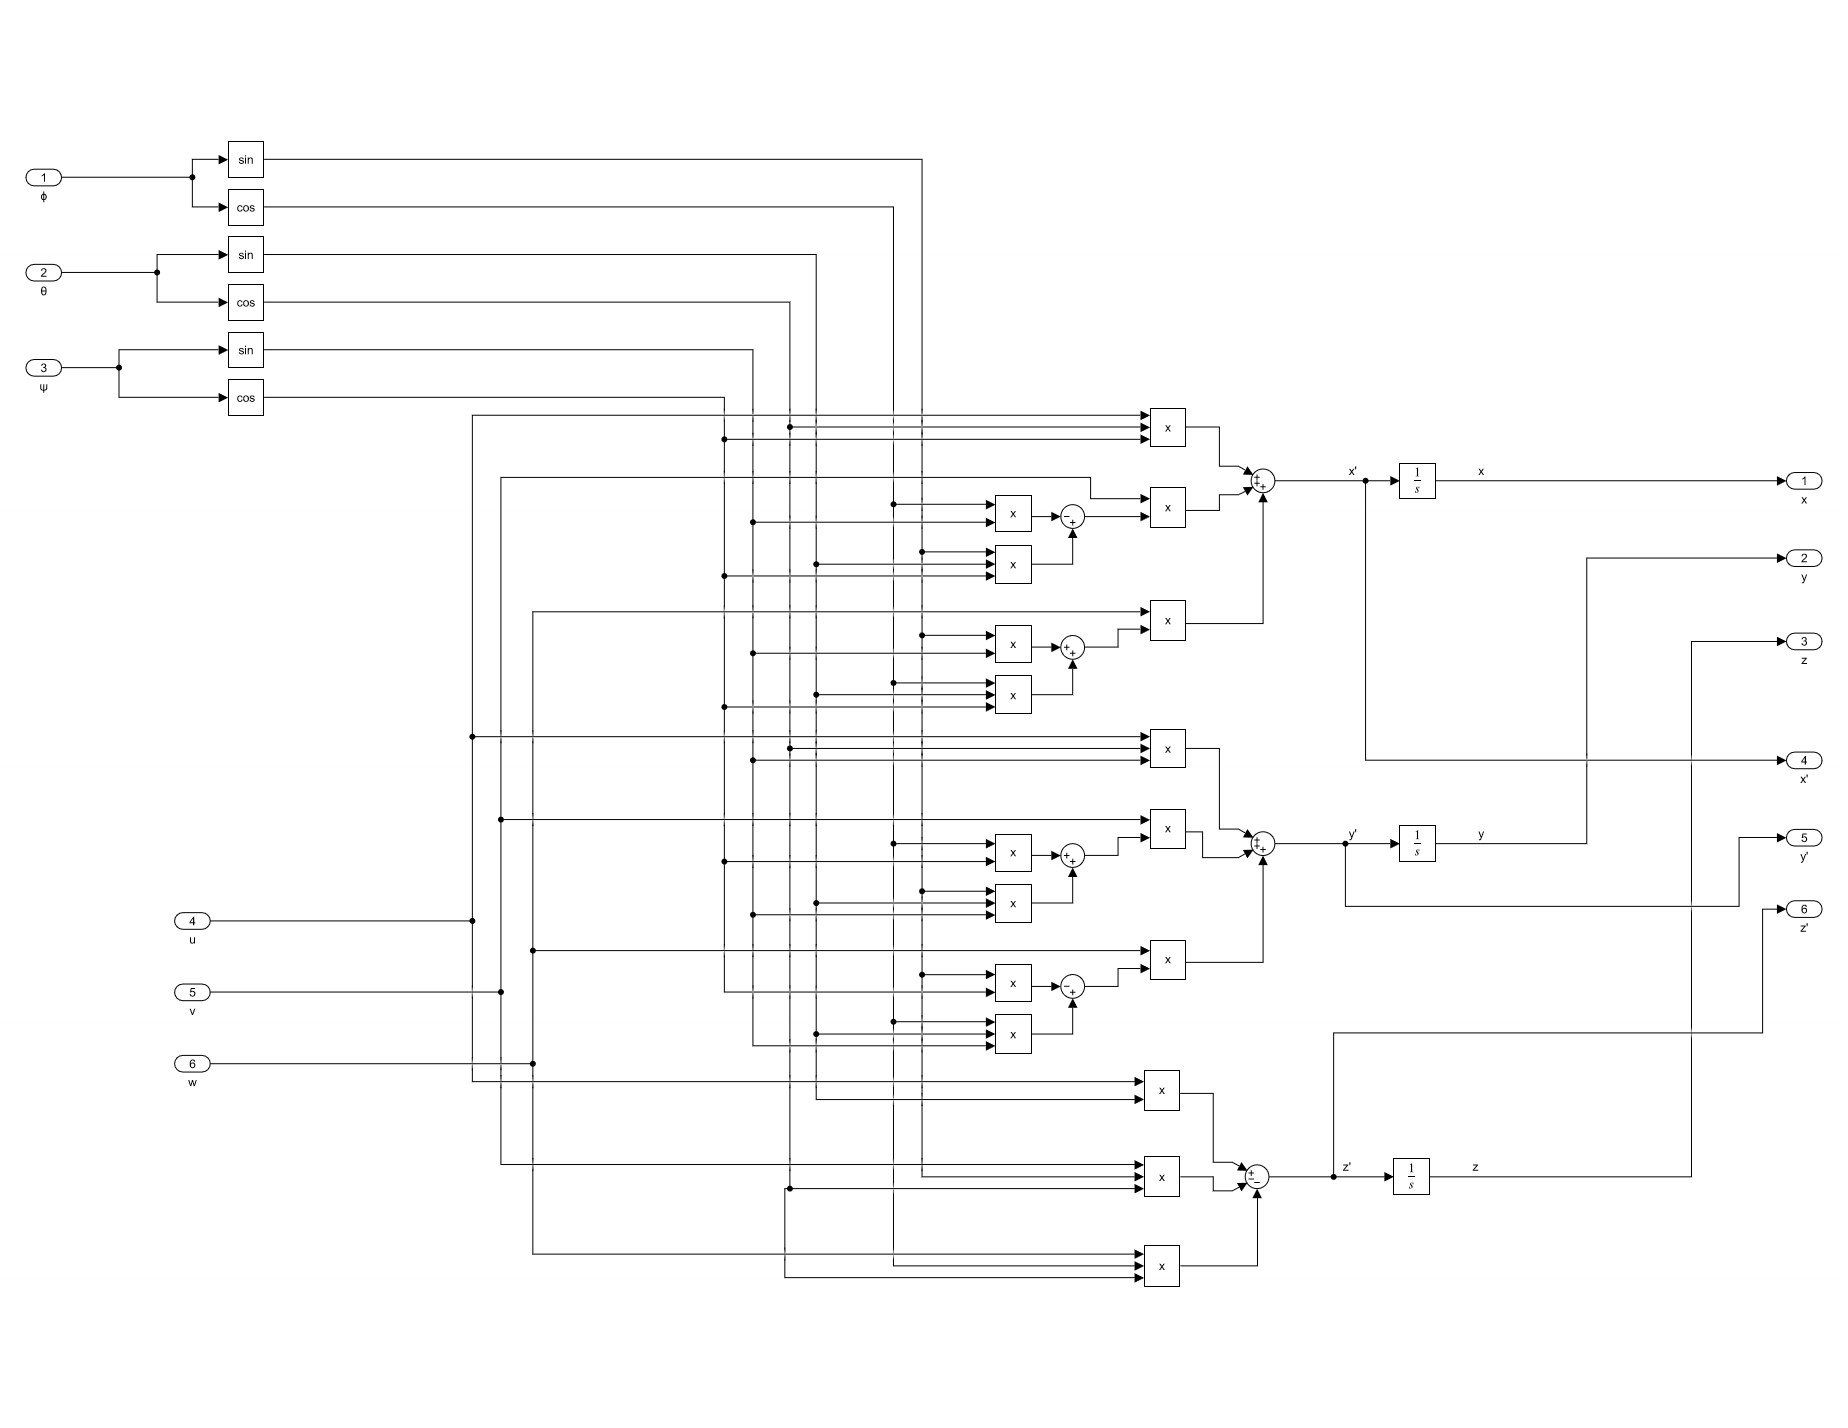
\includegraphics[width=\columnwidth]{/SimulinkModels/Plant/Eq3.6.jpg}%
	\end{center}
	\caption{Equation 3.6 Simulink subsystem.}%	
\end{figure}

\begin{figure}[htb]
\begin{center}
	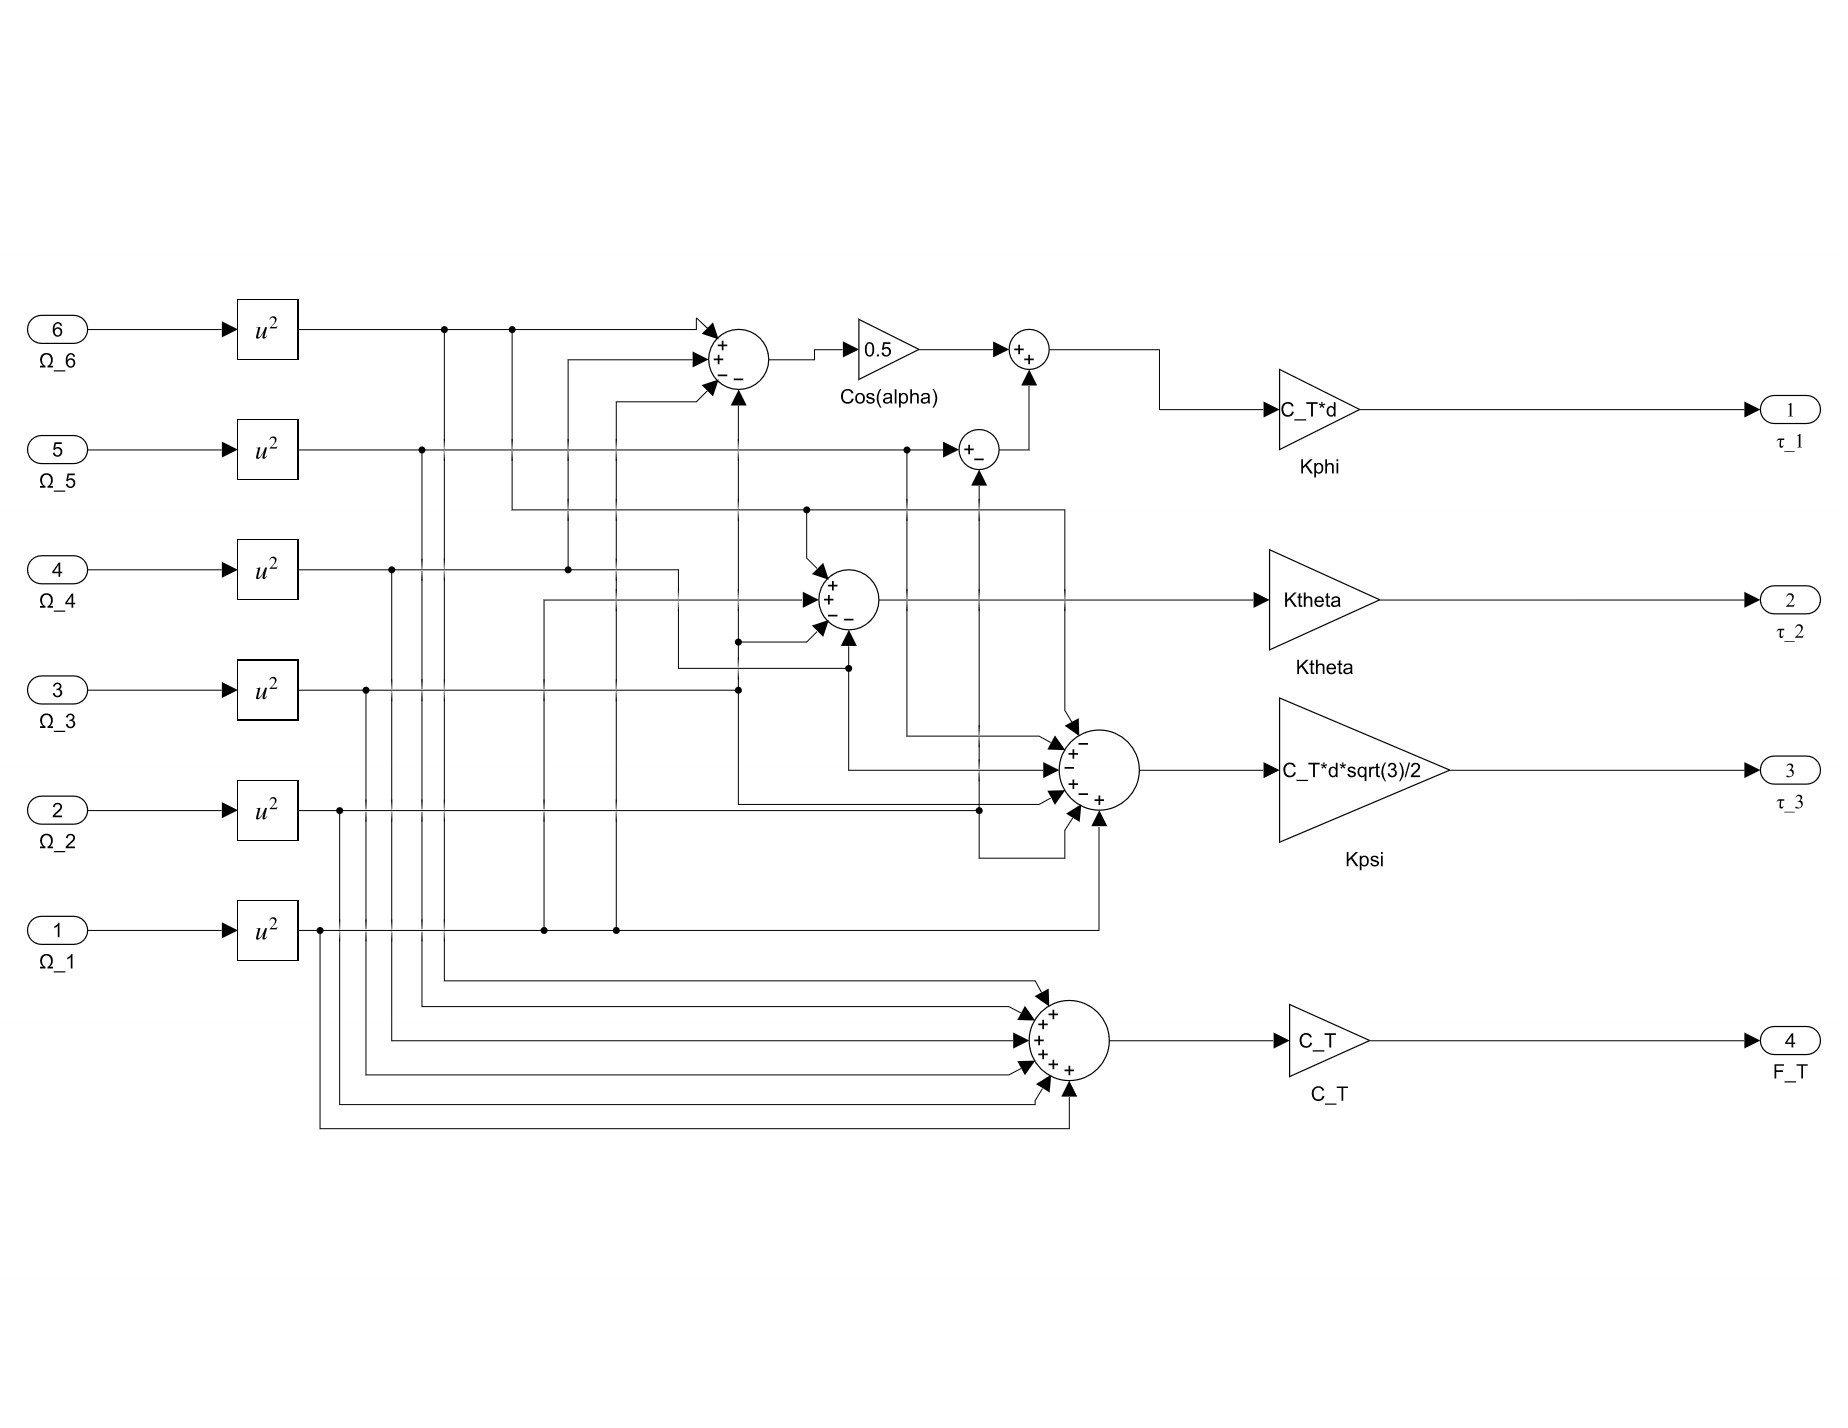
\includegraphics[width=\columnwidth]{/SimulinkModels/Plant/Eq3.9.jpg}%
	\end{center}
	\caption{Equation 3.9 Simulink subsystem.}%	
\end{figure}


\FloatBarrier
\clearpage
\section{Control Inputs to Motor Speeds}

\begin{figure}[htb]
\begin{center}
	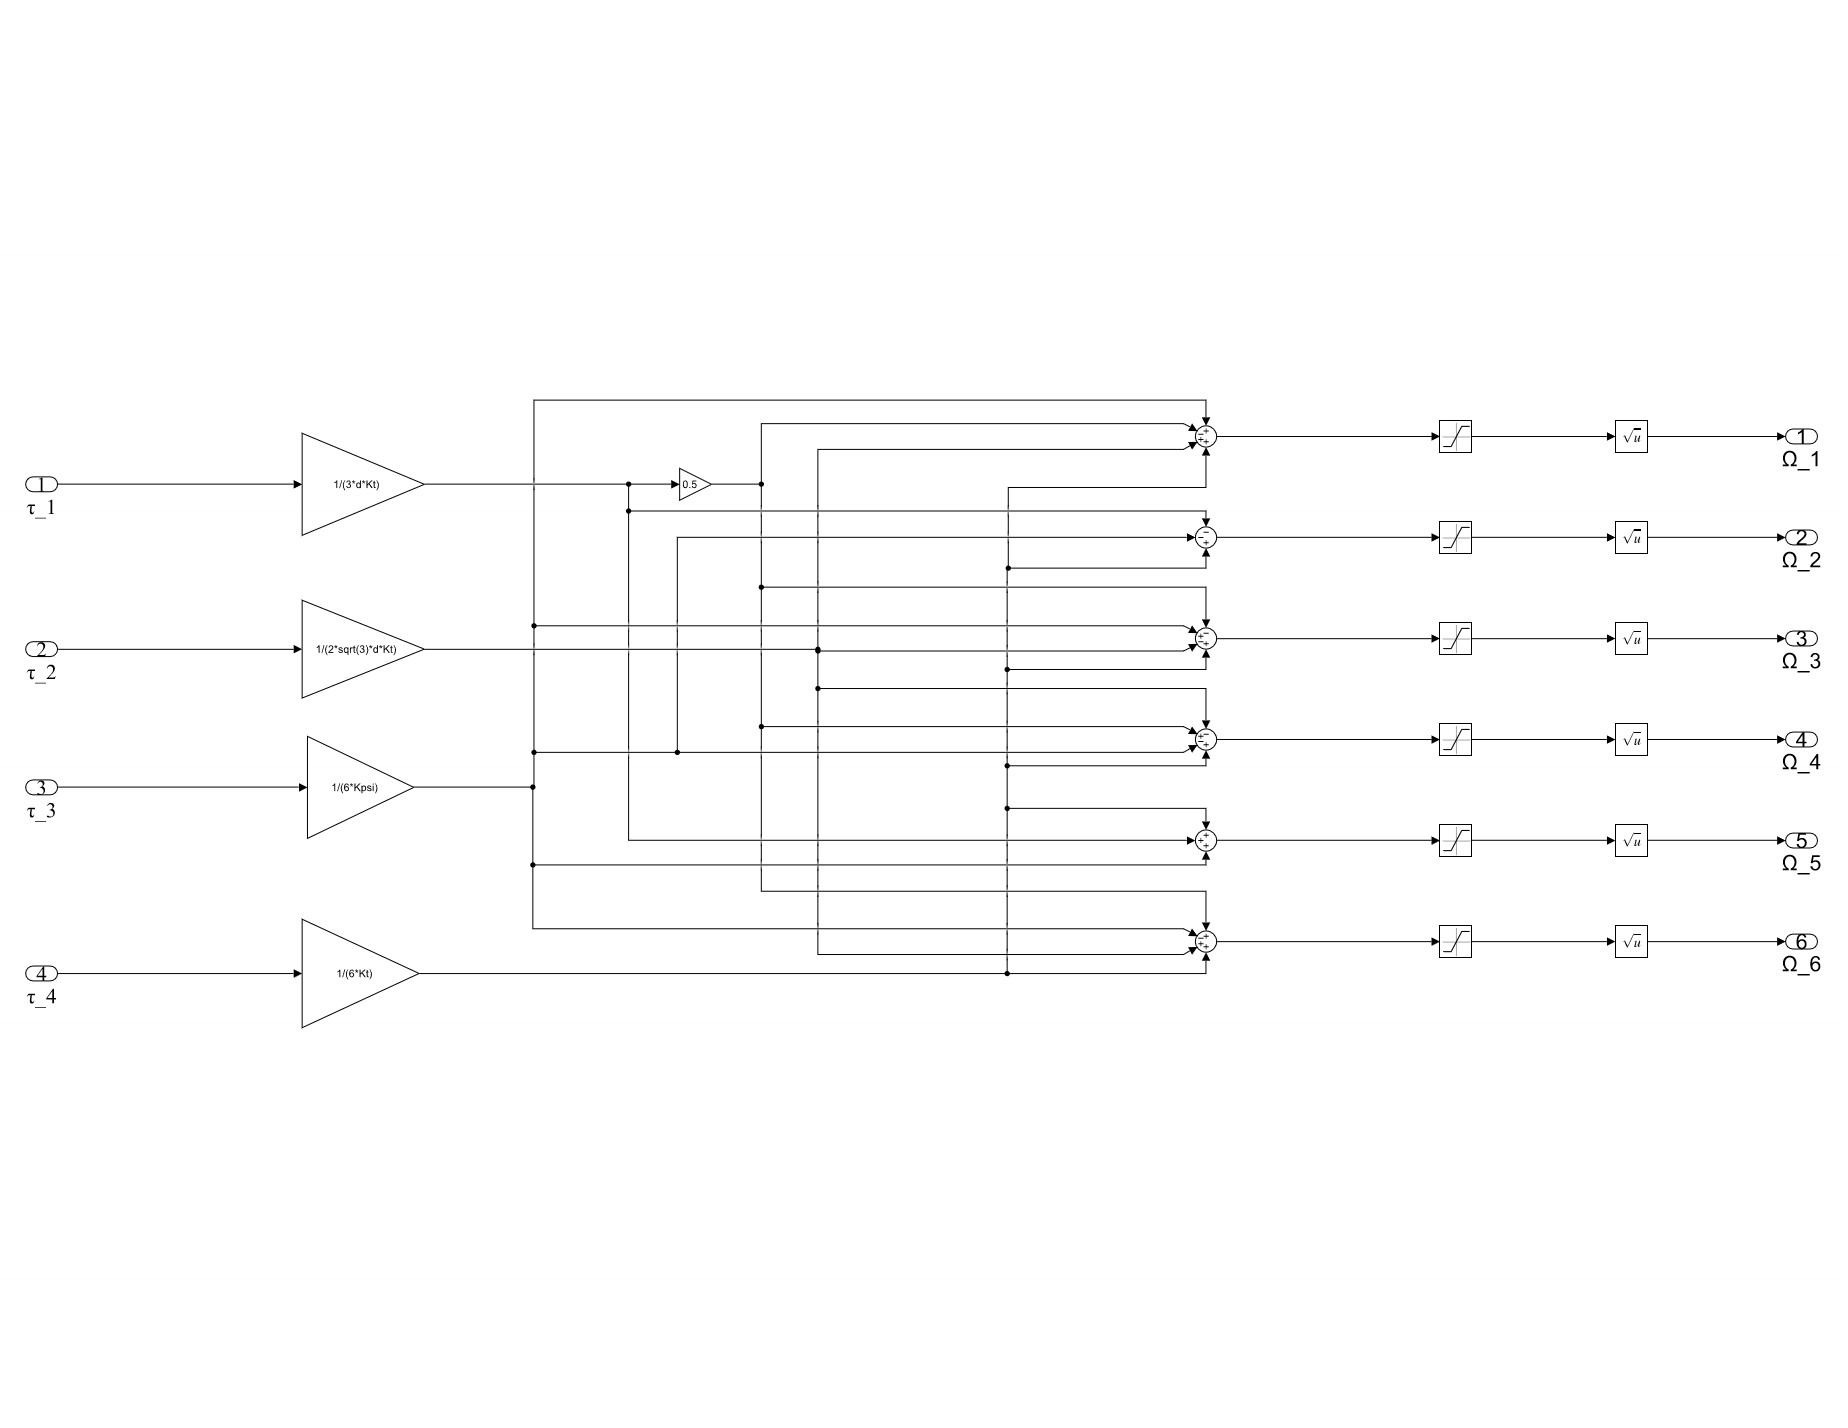
\includegraphics[width=\columnwidth]{/SimulinkModels/InputsToSpeeds.jpg}%
	\end{center}
	\caption{Equation 3.9 Simulink subsystem.}%	
\end{figure}
\FloatBarrier
\clearpage

\section{Control System}

\begin{figure}[htb]
\begin{center}
	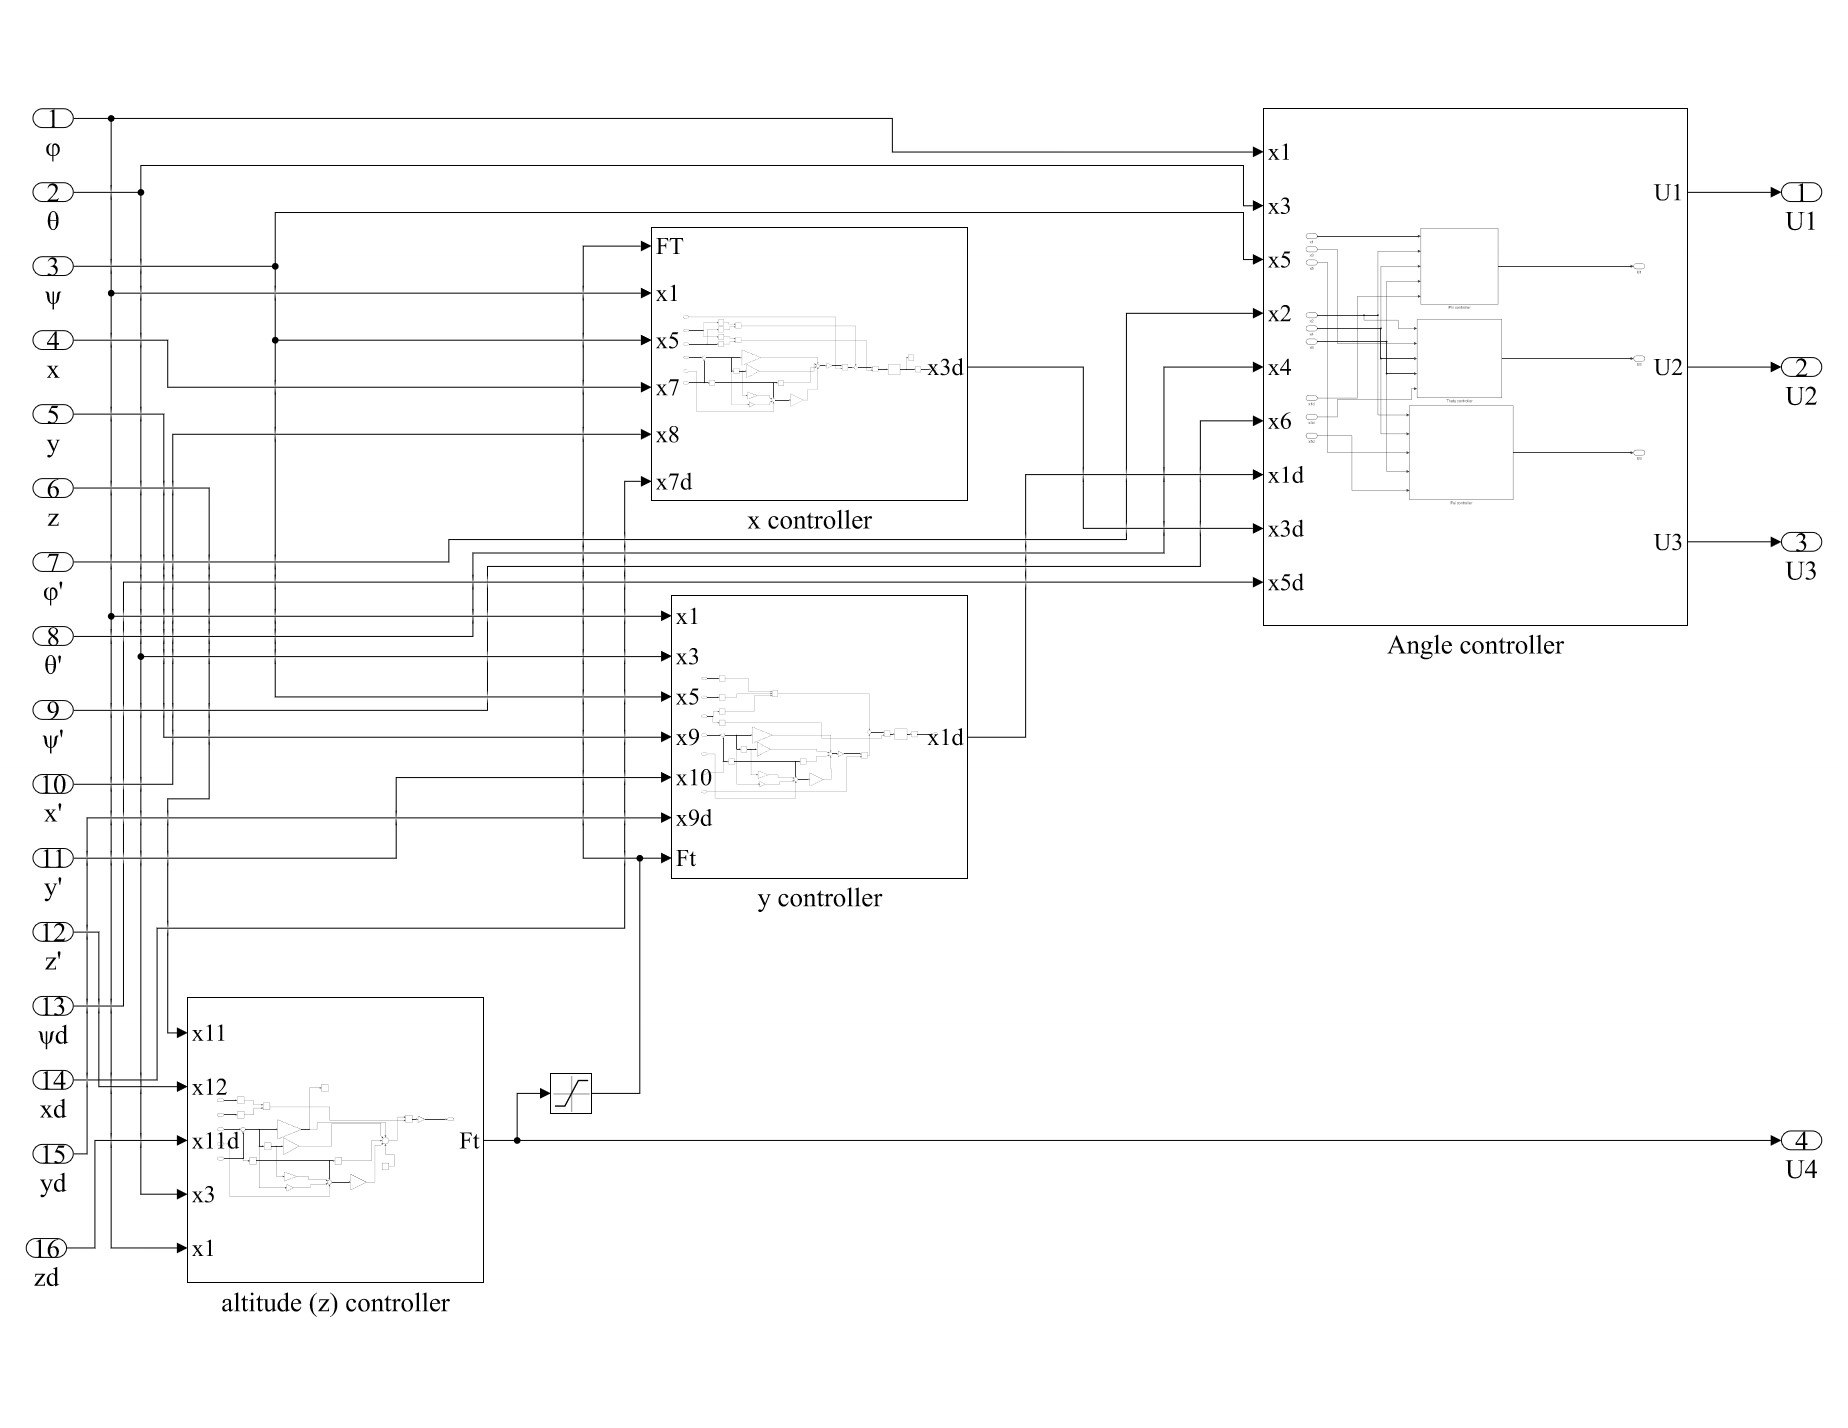
\includegraphics[width=\columnwidth]{/SimulinkModels/Controller/Controller.jpg}%
	\end{center}
	\caption{Control system Simulink model overview.}%
\end{figure}

\begin{figure}[htb]
\begin{center}
	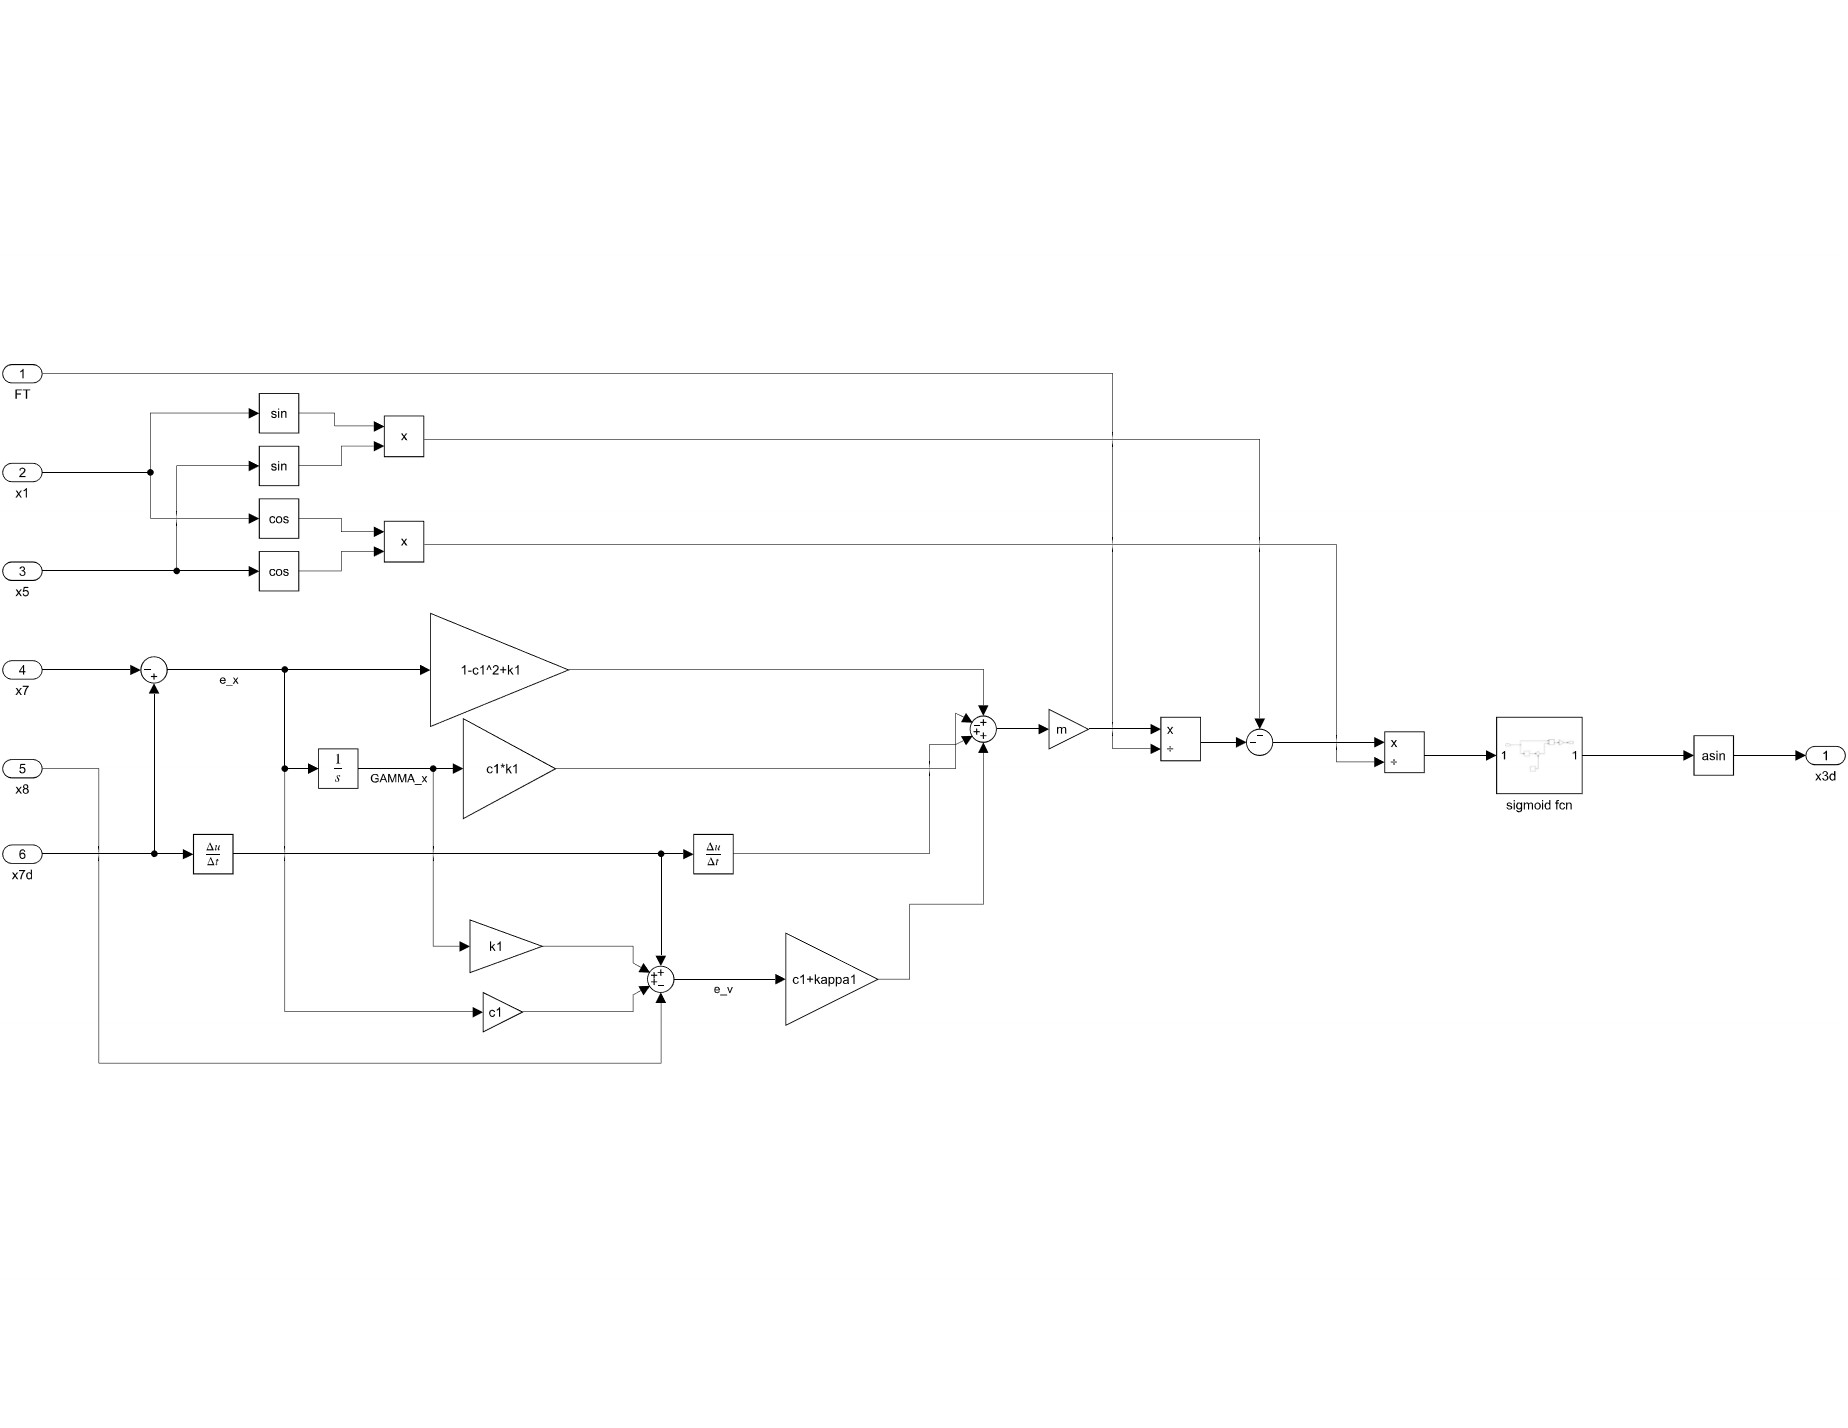
\includegraphics[width=\columnwidth]{/SimulinkModels/Controller/x.jpg}%
	\end{center}
	\caption{X position controller Simulink subsystem.}%
\end{figure}

\begin{figure}[htb]
\begin{center}
	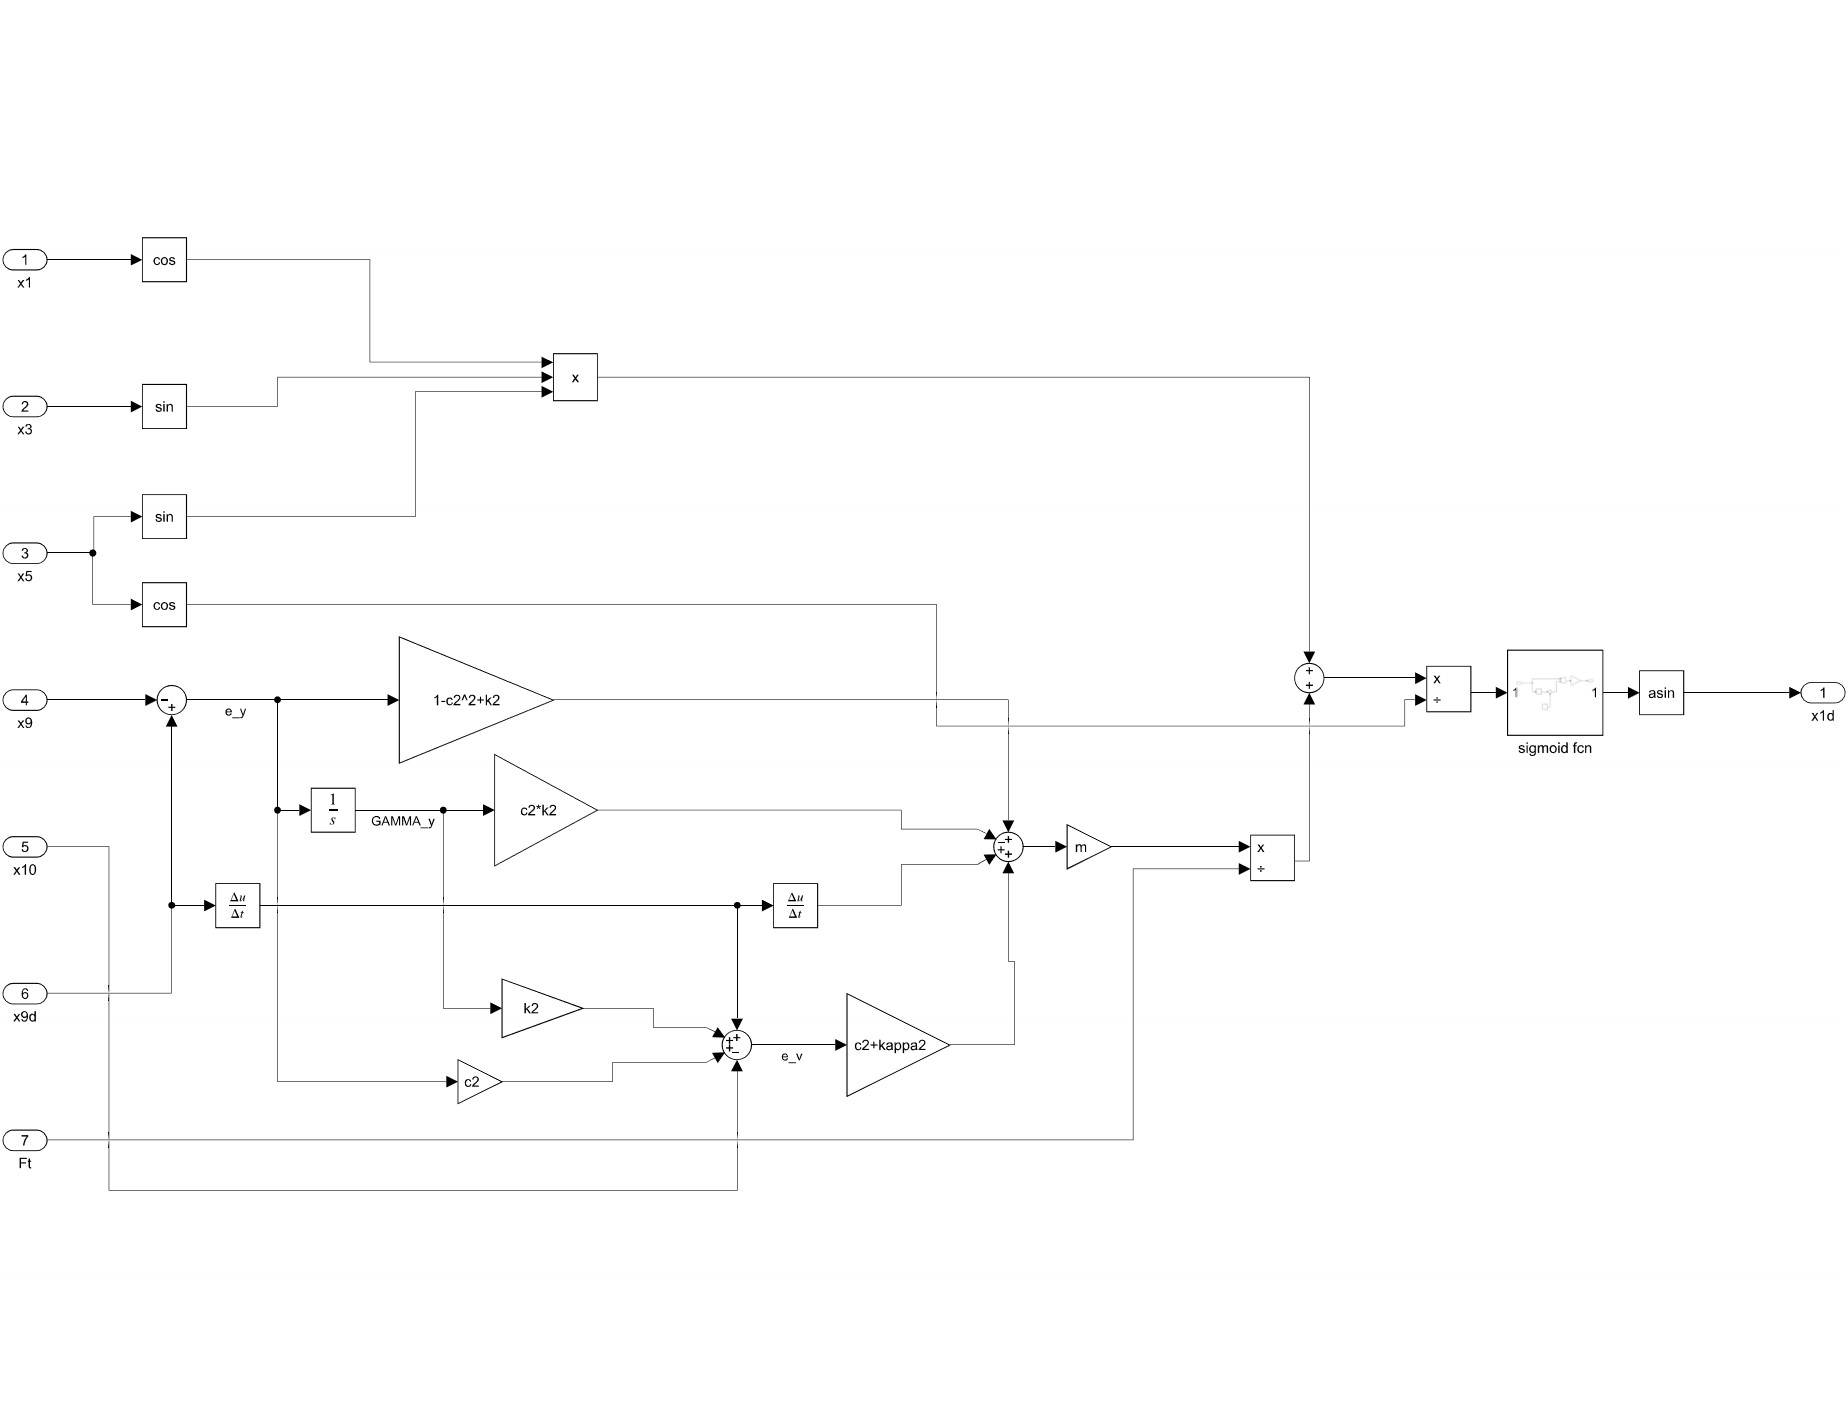
\includegraphics[width=\columnwidth]{/SimulinkModels/Controller/y.jpg}%
	\end{center}
	\caption{Y position controller Simulink subsystem.}%
\end{figure}

\begin{figure}[htb]
\begin{center}
	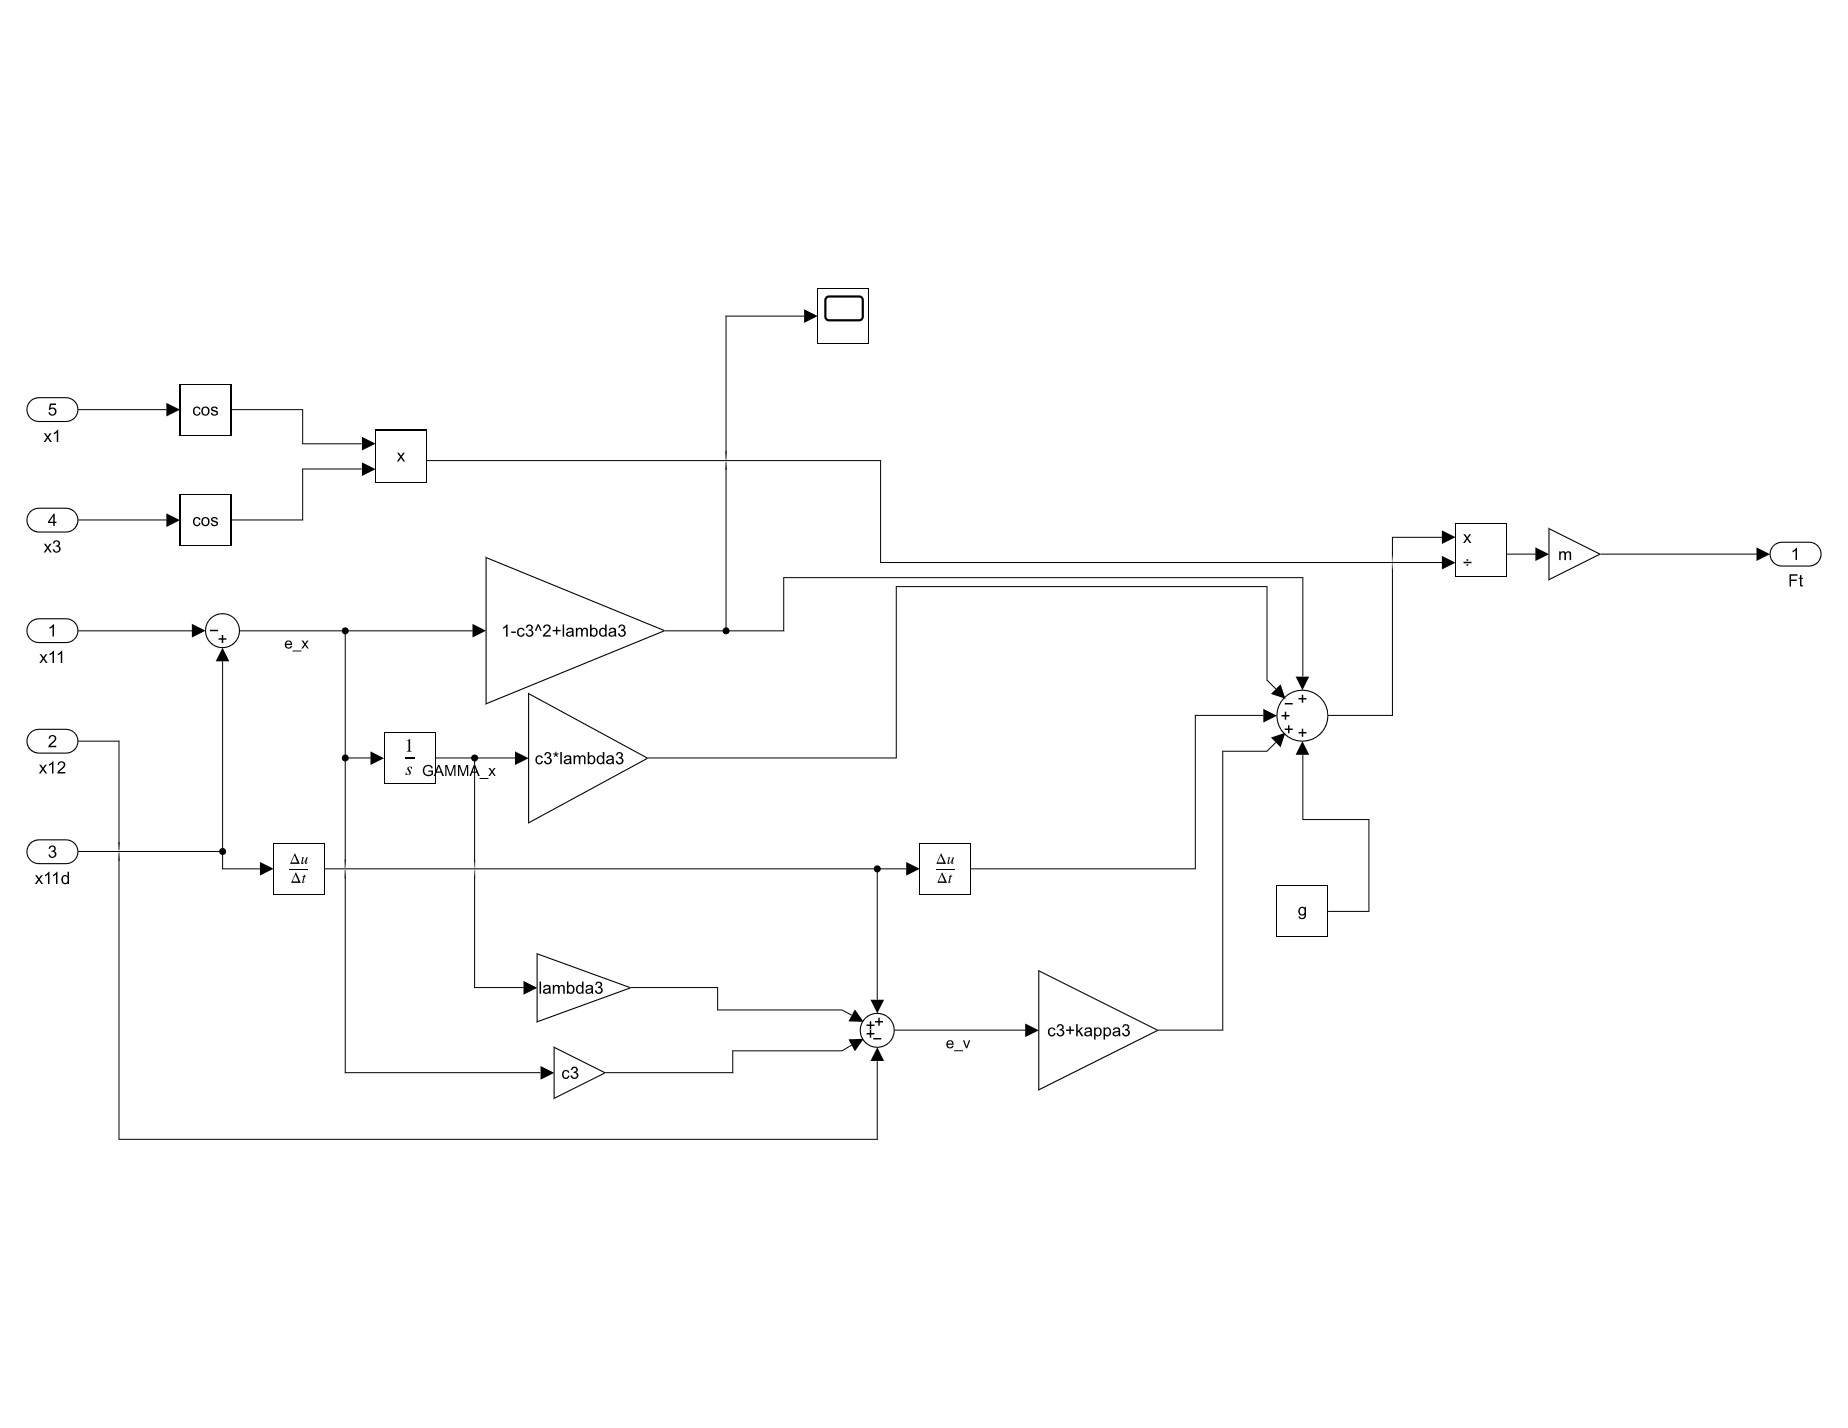
\includegraphics[width=\columnwidth]{/SimulinkModels/Controller/z.jpg}%
	\end{center}
	\caption{Z position controller Simulink subsystem.}%
\end{figure}

\begin{figure}[htb]
\begin{center}
	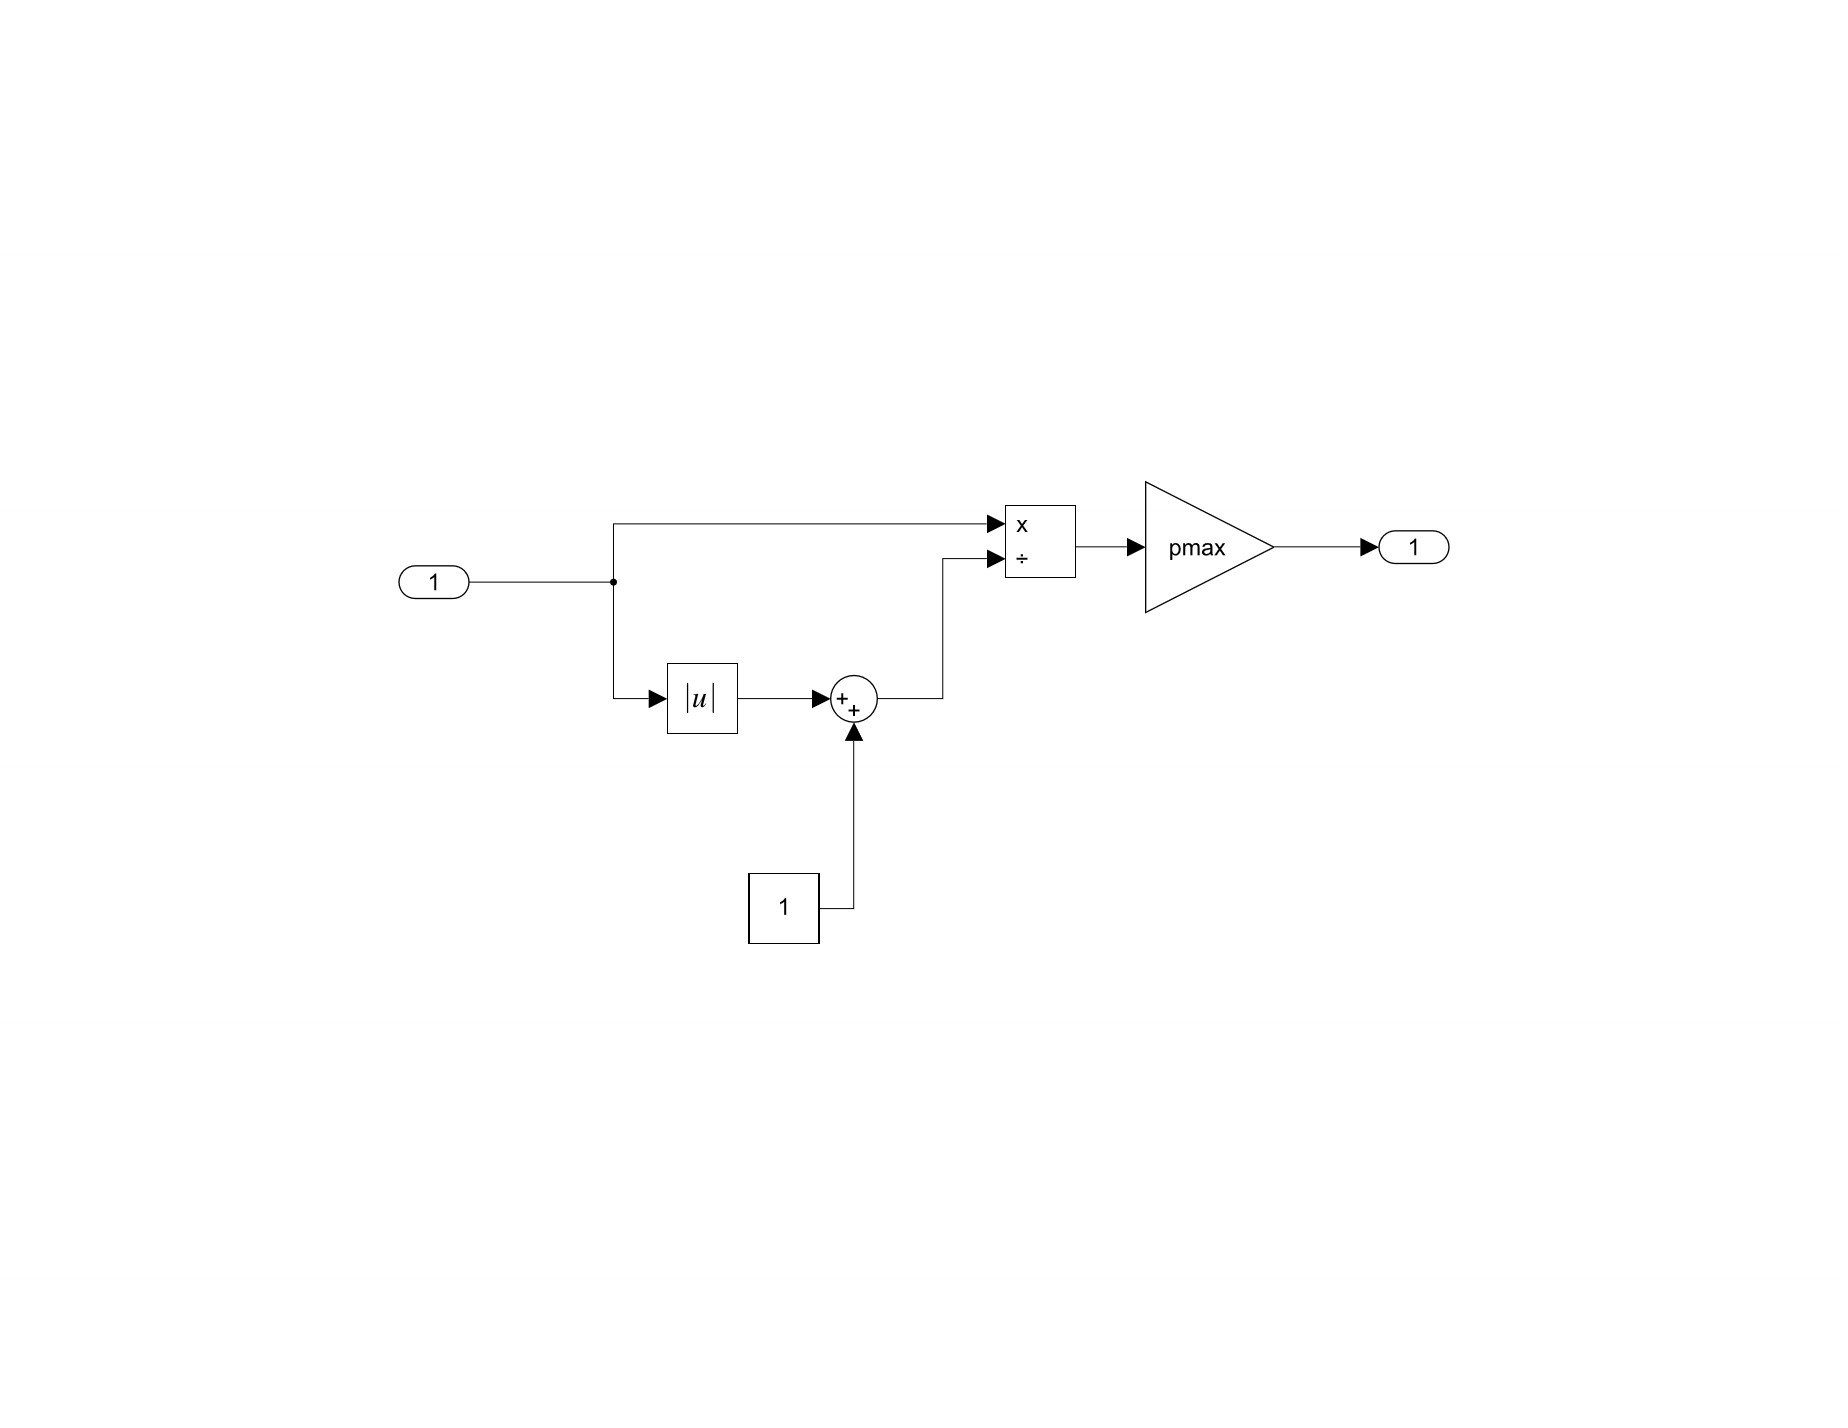
\includegraphics[width=\columnwidth]{/SimulinkModels/Controller/sigmoidal.jpg}%
	\end{center}
	\caption{Sigmoidal function Simulink subsystem.}%
\end{figure}

\begin{figure}[htb]
\begin{center}
	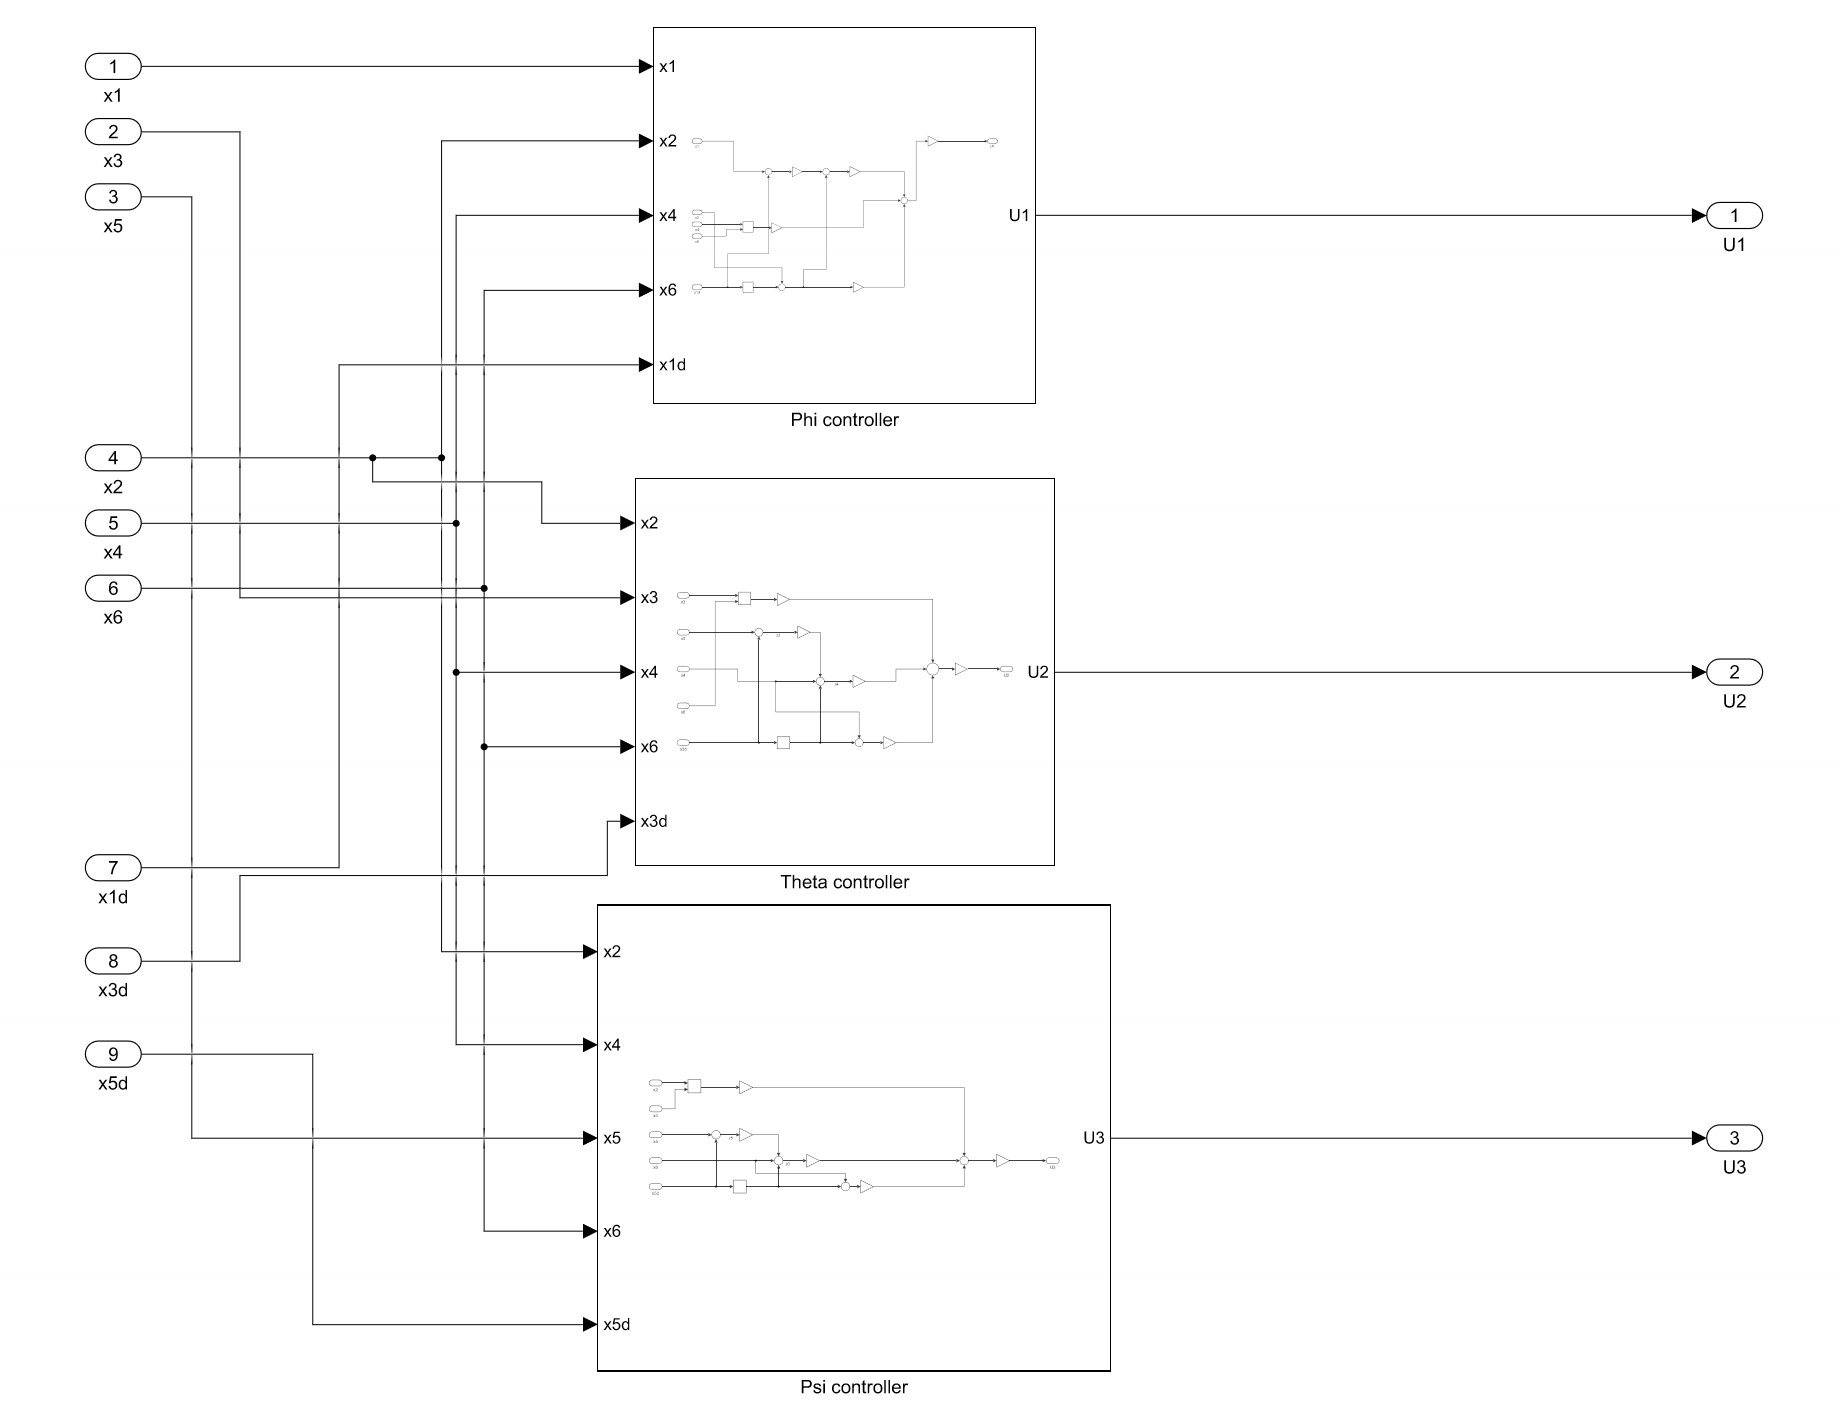
\includegraphics[width=\columnwidth]{/SimulinkModels/Controller/Angle.jpg}%
	\end{center}
	\caption{Angle controller Simulink subsystem.}%
\end{figure}

\begin{figure}[htb]
\begin{center}
	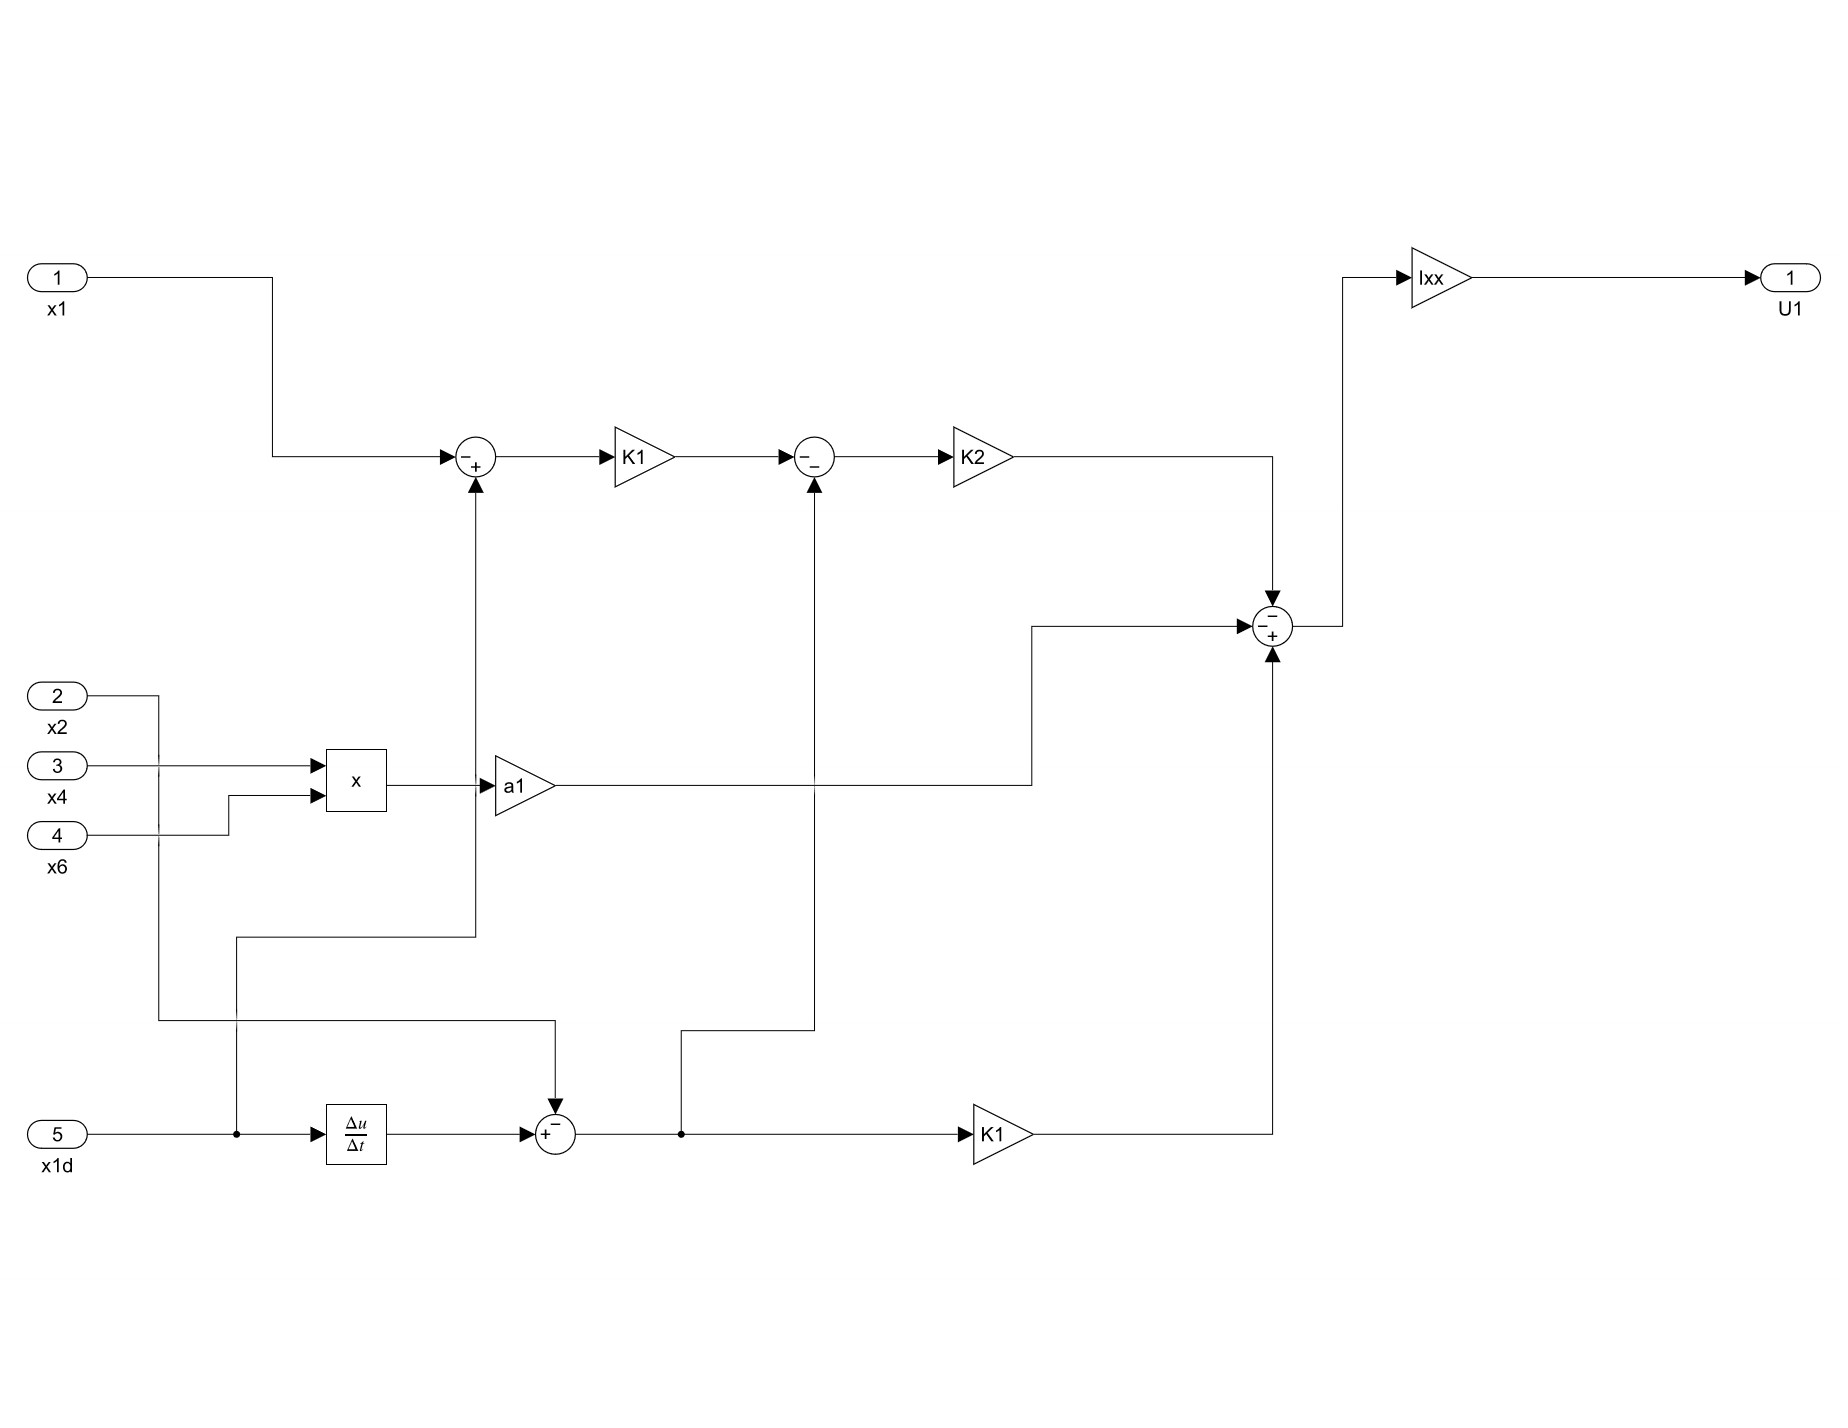
\includegraphics[width=\columnwidth]{/SimulinkModels/Controller/phi.jpg}%
	\end{center}
	\caption{Roll angle controller Simulink subsystem.}%
\end{figure}

\begin{figure}[htb]
\begin{center}
	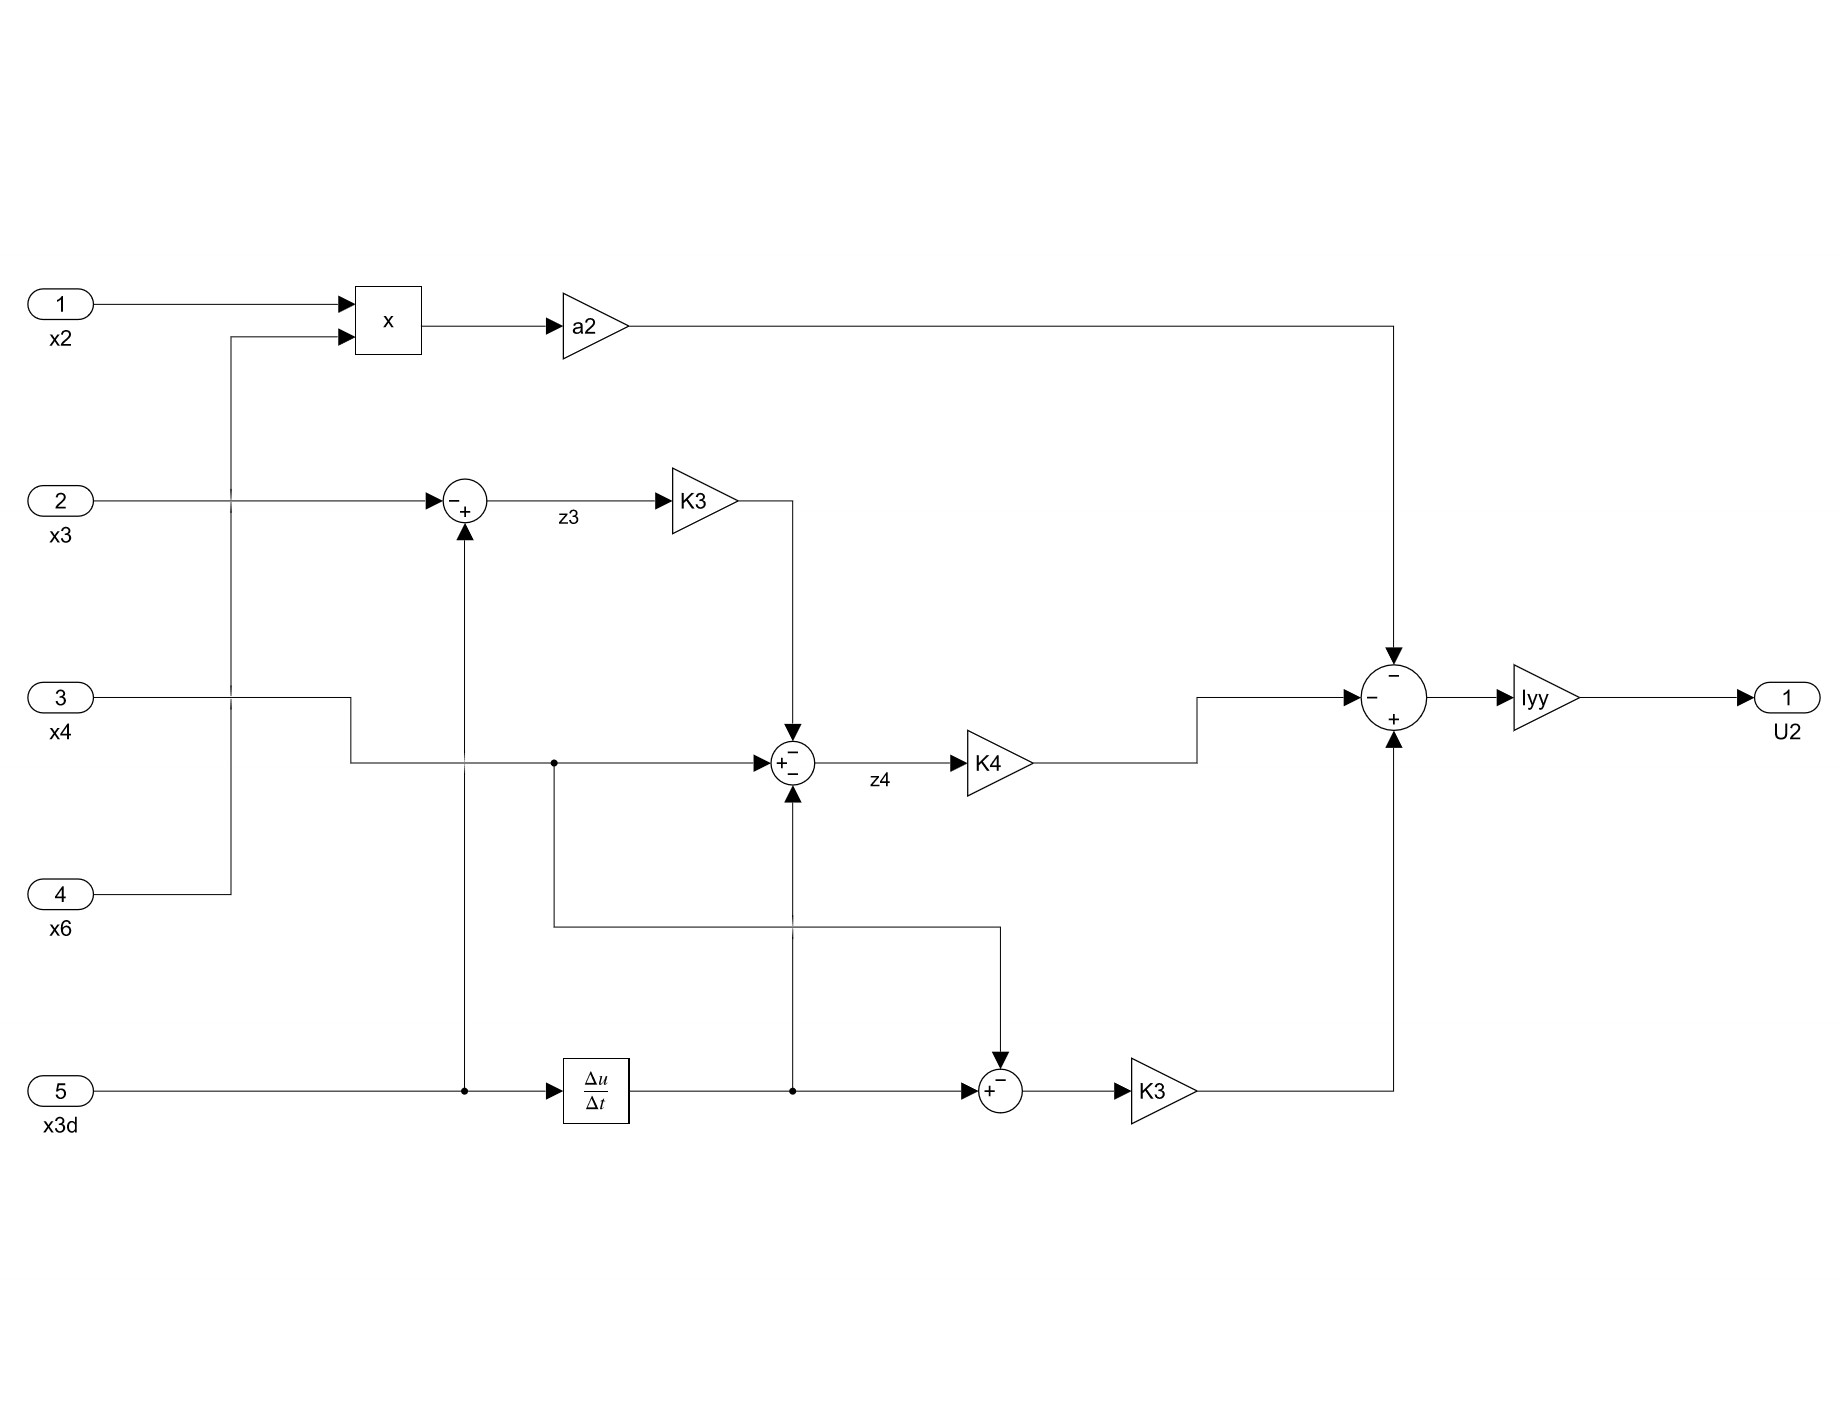
\includegraphics[width=\columnwidth]{/SimulinkModels/Controller/theta.jpg}%
	\end{center}
	\caption{Pitch angle controller Simulink subsystem.}%
\end{figure}

\begin{figure}[htb]
\begin{center}
	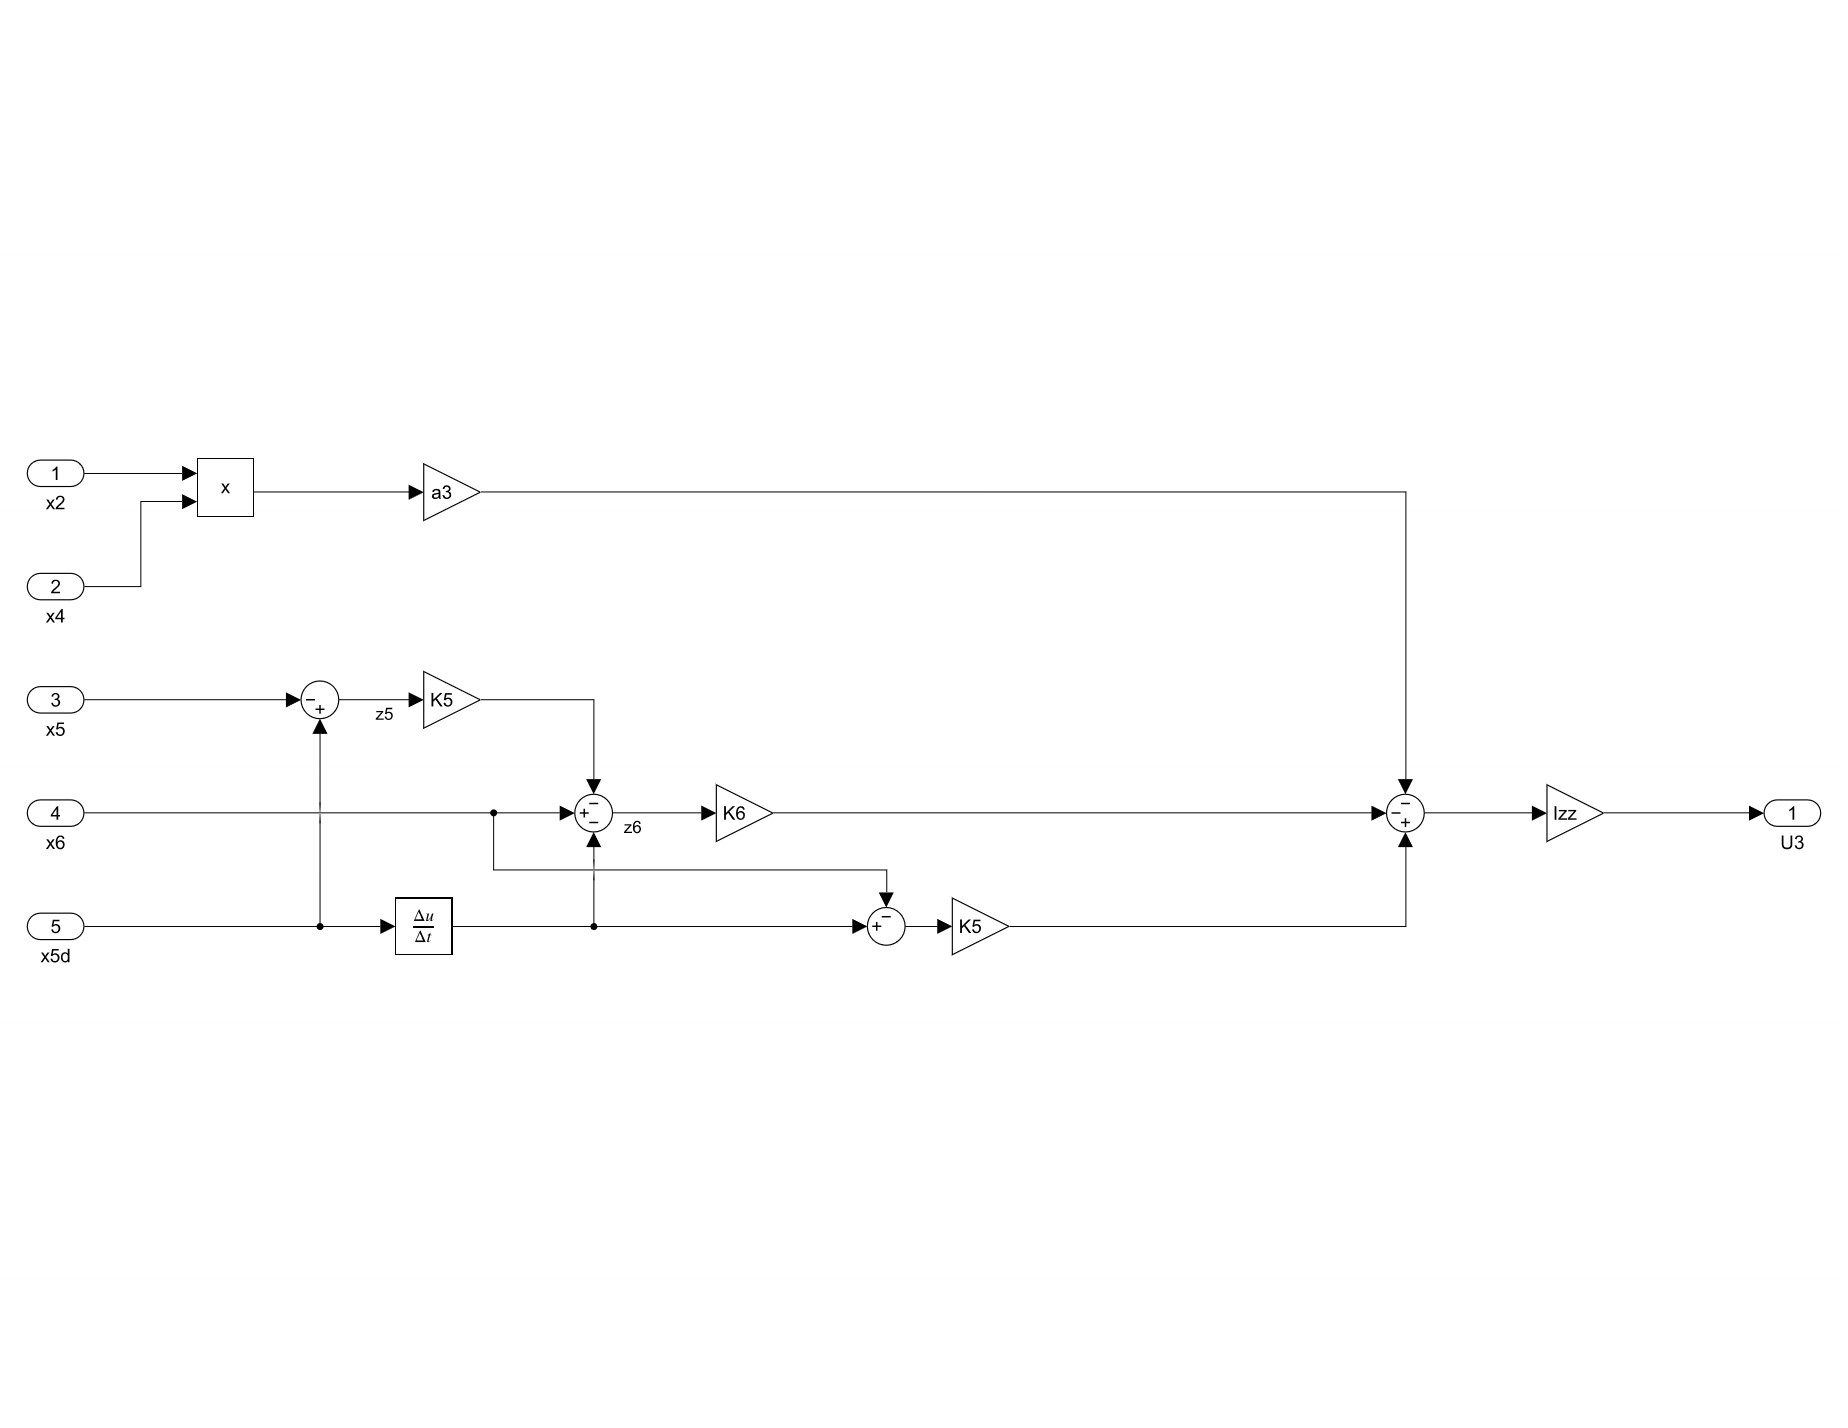
\includegraphics[width=\columnwidth]{/SimulinkModels/Controller/psi.jpg}%
	\end{center}
	\caption{Yaw angle controller Simulink subsystem.}%
\end{figure}

\clearpage
\pagenumbering{arabic}% resets `page` counter to 1
\renewcommand*{\thepage}{B-\arabic{page}}
\chapter{Software Algorithms}
\section{GPS EKF Matlab Code}
\subsection{Script}

% This LaTeX was auto-generated from MATLAB code.
% To make changes, update the MATLAB code and republish this document.


%\usepackage{graphicx}
%\usepackage{color}

%\sloppy
%\definecolor{lightgray}{gray}{0.5}
%\setlength{\parindent}{0pt}

%\begin{document}

    
    \begin{verbatim}
for time=1:(MissionEnd_uS-MissionStart_uS)
    if time==IMU_Data(IMU_count,1)

        x_k_prev=x_k;
        u_k_prev=u_k;
        P_prev=P_k;
        u_k=IMU_Data(IMU_count,2:7);

        %Predict
        x_k=StateTransitionFcn_HW_GPS(x_k_prev,u_k, Ts_IMU);
        F_k=StateJacobian_HW_GPS(x_k_prev,u_k_prev, Ts_IMU);
        P_k=F_k*P_prev*F_k'+Q_k;

        %Update IMU
        z_k=[IMU_Data(IMU_count,2:7)'; z_k(7:16)];
        y_k=z_k-MeasurementFcn_HW_GPS(x_k);
        H_k=MeasurementJacobian_HW_GPS(x_k);
        S_k=H_k*P_k*(H_k')+R_k;
        K_k=(P_k*(H_k'))/S_k;
        x_k=x_k+K_k*y_k;
        P_k=(eye(12)-K_k*H_k)*P_k;

        IMU_count=IMU_count+1;

    end


    if time==Mag_Data(Mag_count,1)
        %Update Mag
        z_k=[z_k(1:6);  Mag_Data(Mag_count,2:4)';z_k(10:16)];
        y_k=z_k-MeasurementFcn_HW_GPS(x_k);
        H_k=MeasurementJacobian_HW_GPS(x_k);
        S_k=H_k*P_k*(H_k')+R_k;
        K_k=(P_k*(H_k'))/S_k;
        x_k=x_k+K_k*y_k;
        P_k=(eye(12)-K_k*H_k)*P_k;

        Mag_count=Mag_count+1;
    end

    if time==GPS_Data(GPS_count,1)
        %Update GPS
        z_k=[z_k(1:9); GPS_Data(GPS_count, 2:7)';z_k(16)];
        y_k=z_k-MeasurementFcn_HW_GPS(x_k);
        H_k=MeasurementJacobian_HW_GPS(x_k);
        S_k=H_k*P_k*(H_k')+R_k;
        K_k=(P_k*(H_k'))/S_k;
        x_k=x_k+K_k*y_k;
        P_k=(eye(12)-K_k*H_k)*P_k;

        GPS_count=GPS_count+1;
    end

    if time==Bar_Data(Bar_count,1)
        %Update Baro
        z_k=[z_k(1:15);Bar_Data(Bar_count, 2)];
        y_k=z_k-MeasurementFcn_HW_GPS(x_k);
        H_k=MeasurementJacobian_HW_GPS(x_k);
        S_k=H_k*P_k*(H_k')+R_k;
        K_k=(P_k*(H_k'))/S_k;
        x_k=x_k+K_k*y_k;
        P_k=(eye(12)-K_k*H_k)*P_k;

        Bar_count=Bar_count+1;
    end

    x_estimated(time, :)=x_k';
end
\end{verbatim}



%\end{document}



\subsection{State Transition Function}

% This LaTeX was auto-generated from MATLAB code.
% To make changes, update the MATLAB code and republish this document.



    
    \begin{verbatim}
function x= StateTransitionFcn_HW_GPS(x,u, Ts)
%Predicts the states of the discretised hexacopter state model at the given x
%and u values

global g;

measAcc=[u(1);u(2);u(3)];
measRate=[u(4);u(5);u(6)];

p=[x(1);x(2);x(3)];
v=[x(4);x(5);x(6)];
PHI=[x(7);x(8);x(9)];
omega=[x(10);x(11);x(12)];

p_new=p+Ts*v;
v_new=v+Ts*([cos(PHI(2))*cos(PHI(3)) (sin(PHI(1))*sin(PHI(2))*cos(PHI(3))-cos(PHI(1))*sin(PHI(3))) (cos(PHI(1))*sin(PHI(2))*cos(PHI(3))+sin(PHI(1))*sin(PHI(3)));
cos(PHI(2))*sin(PHI(3)) (sin(PHI(1))*sin(PHI(2))*sin(PHI(3))+cos(PHI(1))*cos(PHI(3))) (cos(PHI(1))*sin(PHI(2))*sin(PHI(3))-sin(PHI(1))*cos(PHI(3)));
sin(PHI(2)) -sin(PHI(1))*cos(PHI(2)) -cos(PHI(1))*cos(PHI(2))]*(measAcc)+[0;0;g]);

v_new(3)=(p_new(3)-p(3))/Ts;

PHI_new=PHI+Ts*omega;
omega_new=[1 sin(PHI(1))*tan(PHI(2)) cos(PHI(1))*tan(PHI(2));
0 cos(PHI(1)) -sin(PHI(1));
0 sin(PHI(1))*sec(PHI(2)) cos(PHI(1))*sec(PHI(2))]*(measRate);

x=[p_new;v_new;PHI_new;omega_new];

end
\end{verbatim}



\subsection{State Transition Jacobian Function}

% This LaTeX was auto-generated from MATLAB code.
% To make changes, update the MATLAB code and republish this document.



    
    \begin{verbatim}
function F=StateJacobian_HW_GPS(x,u, Ts)
%Evaluates the Jacobian of the discretised hexacopter state model at the given x
%and u values

F =[1, 0, 0, Ts,  0,  0,                                                                                                                     0,                                                                                                         0,                                                                                                                                                  0,  0,  0,  0;
0, 1, 0,  0, Ts,  0,                                                                                                                     0,                                                                                                         0,                                                                                                                                                  0,  0,  0,  0;
0, 0, 1,  0,  0, Ts,                                                                                                                     0,                                                                                                         0,                                                                                                                                                  0,  0,  0,  0;
0, 0, 0,  1,  0,  0,  Ts*((sin(x(7))*sin(x(9)) + cos(x(7))*cos(x(9))*sin(x(8)))*(u(2) ) + (cos(x(7))*sin(x(9)) - cos(x(9))*sin(x(7))*sin(x(8)))*(u(3))), Ts*(cos(x(7))*cos(x(8))*cos(x(9))*(u(3)) - cos(x(9))*sin(x(8))*(u(1)) + cos(x(8))*cos(x(9))*sin(x(7))*(u(2))), -Ts*((cos(x(7))*cos(x(9)) + sin(x(7))*sin(x(8))*sin(x(9)))*(u(2)) - (cos(x(9))*sin(x(7)) - cos(x(7))*sin(x(8))*sin(x(9)))*(u(3)) + cos(x(8))*sin(x(9))*(u(1) )),  0,  0,  0;
0, 0, 0,  0,  1,  0, -Ts*((cos(x(9))*sin(x(7)) - cos(x(7))*sin(x(8))*sin(x(9)))*(u(2) ) + (cos(x(7))*cos(x(9)) + sin(x(7))*sin(x(8))*sin(x(9)))*(u(3))), Ts*(cos(x(7))*cos(x(8))*sin(x(9))*(u(3) ) - sin(x(8))*sin(x(9))*(u(1) ) + cos(x(8))*sin(x(7))*sin(x(9))*(u(2))),  Ts*((sin(x(7))*sin(x(9)) + cos(x(7))*cos(x(9))*sin(x(8)))*(u(3) ) - (cos(x(7))*sin(x(9)) - cos(x(9))*sin(x(7))*sin(x(8)))*(u(2)) + cos(x(8))*cos(x(9))*(u(1))),  0,  0,  0;
0, 0, 0,  0,  0,  1,                                                         -Ts*(cos(x(7))*cos(x(8))*(u(2) ) - cos(x(8))*sin(x(7))*(u(3))),                         Ts*(cos(x(8))*(u(1) ) + cos(x(7))*sin(x(8))*(u(3)) + sin(x(7))*sin(x(8))*(u(2))),                                                                                                                                                  0,  0,  0,  0;
0, 0, 0,  0,  0,  0,                                                                                                                     1,                                                                                                         0,                                                                                                                                                  0, Ts,  0,  0;
0, 0, 0,  0,  0,  0,                                                                                                                     0,                                                                                                         1,                                                                                                                                                  0,  0, Ts,  0;
0, 0, 0,  0,  0,  0,                                                                                                                     0,                                                                                                         0,                                                                                                                                                  1,  0,  0, Ts;
0, 0, 0,  0,  0,  0,                                                               cos(x(7))*tan(x(8))*(u(5) ) - sin(x(7))*tan(x(8))*(u(6)),                                   cos(x(7))*(tan(x(8))^2 + 1)*(u(6)) + sin(x(7))*(tan(x(8))^2 + 1)*(u(5) ),                                                                                                                                                  0,  0,  0,  0;
0, 0, 0,  0,  0,  0,                                                                             - cos(x(7))*(u(6) ) - sin(x(7))*(u(5) ),                                                                                                         0,                                                                                                                                                  0,  0,  0,  0;
0, 0, 0,  0,  0,  0,                                                           (cos(x(7))*(u(5) ))/cos(x(8)) - (sin(x(7))*(u(6)))/cos(x(8)),                           (cos(x(7))*sin(x(8))*(u(6)))/cos(x(8))^2 + (sin(x(7))*sin(x(8))*(u(5) ))/cos(x(8))^2,                                                                                                                                                  0,  0,  0,  0;];


end
\end{verbatim}
   


\subsection{Measurement Function}

% This LaTeX was auto-generated from MATLAB code.
% To make changes, update the MATLAB code and republish this document.


    
    \begin{verbatim}
function h=MeasurementFcn_HW_GPS(x)
%Uses the given state to predict the current measurements

global g mag_x mag_y mag_z;


%IMU measurements

a=[-sin(x(8))*g;sin(x(7))*cos(x(8))*g;-cos(x(7))*cos(x(8))*g];

omega=[1 0 -sin(x(8));
       0 cos(x(7)) sin(x(7))*cos(x(8));
       0 -sin(x(7)) cos(x(7))*cos(x(8))]*[x(10);x(11);x(12)];
%Magnetometer
mag=[cos(x(8))*cos(x(9)) cos(x(8))*sin(x(9)) sin(x(8));
sin(x(7))*sin(x(8))*cos(x(9))-cos(x(7))*sin(x(9)) sin(x(7))*sin(x(8))*sin(x(9))+cos(x(7))*cos(x(9)) -sin(x(7))*cos(x(8));
cos(x(7))*sin(x(8))*cos(x(9))+sin(x(7))*sin(x(9)) cos(x(7))*sin(x(8))*sin(x(9))-sin(x(7))*cos(x(9)) -cos(x(7))*cos(x(8))]*[mag_x;mag_y;mag_z];

%GPS/baro
position=[x(1); x(2);x(3)];
velocity=[x(4);x(5);x(6)];

z_bar=x(3);

h=[a;omega;mag;position;velocity; z_bar];

end
\end{verbatim}

      

\subsection{Measurement Jacobian Function}

% This LaTeX was auto-generated from MATLAB code.
% To make changes, update the MATLAB code and republish this document.


    
    \begin{verbatim}
function H=MeasurementJacobian_HW_GPS(x)
%Evaluates the systems measurement Jacobian at the given x

global g mag_x mag_y mag_z;
H=[0, 0, 0, 0, 0, 0,                                                                                                                                                                                                                       0,                                                                                                                                  -cos(conj(x(8)))*conj(g),                                                                                                                                                                               0, 0,              0,                           0;
0, 0, 0, 0, 0, 0,                                                                                                                                                                                     cos(conj(x(7)))*cos(conj(x(8)))*conj(g),                                                                                                                    -sin(conj(x(7)))*sin(conj(x(8)))*conj(g),                                                                                                                                                                               0, 0,              0,                           0;
0, 0, 0, 0, 0, 0,                                                                                                                                                                                     cos(conj(x(8)))*sin(conj(x(7)))*conj(g),                                                                                                                     cos(conj(x(7)))*sin(conj(x(8)))*conj(g),                                                                                                                                                                               0, 0,              0,                           0;
0, 0, 0, 0, 0, 0,                                                                                                                                                                                                                       0,                                                                                                                                -cos(conj(x(8)))*conj(x(12)),                                                                                                                                                                               0, 1,              0,              -sin(conj(x(8)));
0, 0, 0, 0, 0, 0,                                                                                                                                                         cos(conj(x(7)))*cos(conj(x(8)))*conj(x(12)) - sin(conj(x(7)))*conj(x(11)),                                                                                                                  -sin(conj(x(7)))*sin(conj(x(8)))*conj(x(12)),                                                                                                                                                                               0, 0,  cos(conj(x(7))), cos(conj(x(8)))*sin(conj(x(7)));
0, 0, 0, 0, 0, 0,                                                                                                                                                       - cos(conj(x(7)))*conj(x(11)) - cos(conj(x(8)))*sin(conj(x(7)))*conj(x(12)),                                                                                                                  -cos(conj(x(7)))*sin(conj(x(8)))*conj(x(12)),                                                                                                                                                                               0, 0, -sin(conj(x(7))), cos(conj(x(7)))*cos(conj(x(8)));
0, 0, 0, 0, 0, 0,                                                                                                                                                                                                                       0,                                           cos(conj(x(8)))*conj(mag_z) - cos(conj(x(9)))*sin(conj(x(8)))*conj(mag_x) - sin(conj(x(8)))*sin(conj(x(9)))*conj(mag_y),                                                                                               cos(conj(x(8)))*cos(conj(x(9)))*conj(mag_y) - cos(conj(x(8)))*sin(conj(x(9)))*conj(mag_x), 0,              0,                           0;
0, 0, 0, 0, 0, 0, conj(mag_x)*(sin(conj(x(7)))*sin(conj(x(9))) + cos(conj(x(7)))*cos(conj(x(9)))*sin(conj(x(8)))) - conj(mag_y)*(cos(conj(x(9)))*sin(conj(x(7))) - cos(conj(x(7)))*sin(conj(x(8)))*sin(conj(x(9)))) - cos(conj(x(7)))*cos(conj(x(8)))*conj(mag_z), sin(conj(x(7)))*sin(conj(x(8)))*conj(mag_z) + cos(conj(x(8)))*sin(conj(x(7)))*sin(conj(x(9)))*conj(mag_y) + cos(conj(x(8)))*cos(conj(x(9)))*sin(conj(x(7)))*conj(mag_x), - conj(mag_x)*(cos(conj(x(7)))*cos(conj(x(9))) + sin(conj(x(7)))*sin(conj(x(8)))*sin(conj(x(9)))) - conj(mag_y)*(cos(conj(x(7)))*sin(conj(x(9))) - cos(conj(x(9)))*sin(conj(x(7)))*sin(conj(x(8)))), 0,              0,                           0;
0, 0, 0, 0, 0, 0, conj(mag_x)*(cos(conj(x(7)))*sin(conj(x(9))) - cos(conj(x(9)))*sin(conj(x(7)))*sin(conj(x(8)))) - conj(mag_y)*(cos(conj(x(7)))*cos(conj(x(9))) + sin(conj(x(7)))*sin(conj(x(8)))*sin(conj(x(9)))) + cos(conj(x(8)))*sin(conj(x(7)))*conj(mag_z), cos(conj(x(7)))*sin(conj(x(8)))*conj(mag_z) + cos(conj(x(7)))*cos(conj(x(8)))*cos(conj(x(9)))*conj(mag_x) + cos(conj(x(7)))*cos(conj(x(8)))*sin(conj(x(9)))*conj(mag_y),   conj(mag_x)*(cos(conj(x(9)))*sin(conj(x(7))) - cos(conj(x(7)))*sin(conj(x(8)))*sin(conj(x(9)))) + conj(mag_y)*(sin(conj(x(7)))*sin(conj(x(9))) + cos(conj(x(7)))*cos(conj(x(9)))*sin(conj(x(8)))), 0,              0,                           0;
1, 0, 0, 0, 0, 0,                                                                                                                                                                                                                       0,                                                                                                                                                       0,                                                                                                                                                                               0, 0,              0,                           0;
0, 1, 0, 0, 0, 0,                                                                                                                                                                                                                       0,                                                                                                                                                       0,                                                                                                                                                                               0, 0,              0,                           0;
0, 0, 1, 0, 0, 0,                                                                                                                                                                                                                       0,                                                                                                                                                       0,                                                                                                                                                                               0, 0,              0,                           0;
0, 0, 0, 1, 0, 0,                                                                                                                                                                                                                       0,                                                                                                                                                       0,                                                                                                                                                                               0, 0,              0,                           0;
0, 0, 0, 0, 1, 0,                                                                                                                                                                                                                       0,                                                                                                                                                       0,                                                                                                                                                                               0, 0,              0,                           0;
0, 0, 0, 0, 0, 1,                                                                                                                                                                                                                       0,                                                                                                                                                       0,                                                                                                                                                                               0, 0,              0,                           0;
0, 0, 1, 0, 0, 0,                                                                                                                                                                                                                       0,                                                                                                                                                       0,                                                                                                                                                                               0, 0,              0,                           0];
end
\end{verbatim}




\section{OFS EKF Matlab Code}
\subsection{Script}
%
% This LaTeX was auto-generated from MATLAB code.
% To make changes, update the MATLAB code and republish this document.


%\usepackage{graphicx}
%\usepackage{color}

%\sloppy
%\definecolor{lightgray}{gray}{0.5}
%\setlength{\parindent}{0pt}

%\begin{document}

    
    \begin{verbatim}
for time=1:(MissionEnd_uS-MissionStart_uS)
    if time==IMU_Data(IMU_count,1)

        x_k_prev=x_k;
        u_k_prev=u_k;
        P_prev=P_k;
        u_k=IMU_Data(IMU_count,2:7);

        %Predict
        x_k=StateTransitionFcn_HW_GPS(x_k_prev,u_k, Ts_IMU);
        F_k=StateJacobian_HW_GPS(x_k_prev,u_k_prev, Ts_IMU);
        P_k=F_k*P_prev*F_k'+Q_k;

        %Update IMU
        z_k=[IMU_Data(IMU_count,2:7)'; z_k(7:16)];
        y_k=z_k-MeasurementFcn_HW_GPS(x_k);
        H_k=MeasurementJacobian_HW_GPS(x_k);
        S_k=H_k*P_k*(H_k')+R_k;
        K_k=(P_k*(H_k'))/S_k;
        x_k=x_k+K_k*y_k;
        P_k=(eye(12)-K_k*H_k)*P_k;

        IMU_count=IMU_count+1;

    end


    if time==Mag_Data(Mag_count,1)
        %Update Mag
        z_k=[z_k(1:6);  Mag_Data(Mag_count,2:4)';z_k(10:16)];
        y_k=z_k-MeasurementFcn_HW_GPS(x_k);
        H_k=MeasurementJacobian_HW_GPS(x_k);
        S_k=H_k*P_k*(H_k')+R_k;
        K_k=(P_k*(H_k'))/S_k;
        x_k=x_k+K_k*y_k;
        P_k=(eye(12)-K_k*H_k)*P_k;

        Mag_count=Mag_count+1;
    end

    if time==GPS_Data(GPS_count,1)
        %Update GPS
        z_k=[z_k(1:9); GPS_Data(GPS_count, 2:7)';z_k(16)];
        y_k=z_k-MeasurementFcn_HW_GPS(x_k);
        H_k=MeasurementJacobian_HW_GPS(x_k);
        S_k=H_k*P_k*(H_k')+R_k;
        K_k=(P_k*(H_k'))/S_k;
        x_k=x_k+K_k*y_k;
        P_k=(eye(12)-K_k*H_k)*P_k;

        GPS_count=GPS_count+1;
    end

    if time==Bar_Data(Bar_count,1)
        %Update Baro
        z_k=[z_k(1:15);Bar_Data(Bar_count, 2)];
        y_k=z_k-MeasurementFcn_HW_GPS(x_k);
        H_k=MeasurementJacobian_HW_GPS(x_k);
        S_k=H_k*P_k*(H_k')+R_k;
        K_k=(P_k*(H_k'))/S_k;
        x_k=x_k+K_k*y_k;
        P_k=(eye(12)-K_k*H_k)*P_k;

        Bar_count=Bar_count+1;
    end

    x_estimated(time, :)=x_k';
end
\end{verbatim}



%\end{document}


\subsection{State Transition Function}
%
% This LaTeX was auto-generated from MATLAB code.
% To make changes, update the MATLAB code and republish this document.



    
    \begin{verbatim}
function x= StateTransitionFcn_HW_GPS(x,u, Ts)
%Predicts the states of the discretised hexacopter state model at the given x
%and u values

global g;

measAcc=[u(1);u(2);u(3)];
measRate=[u(4);u(5);u(6)];

p=[x(1);x(2);x(3)];
v=[x(4);x(5);x(6)];
PHI=[x(7);x(8);x(9)];
omega=[x(10);x(11);x(12)];

p_new=p+Ts*v;
v_new=v+Ts*([cos(PHI(2))*cos(PHI(3)) (sin(PHI(1))*sin(PHI(2))*cos(PHI(3))-cos(PHI(1))*sin(PHI(3))) (cos(PHI(1))*sin(PHI(2))*cos(PHI(3))+sin(PHI(1))*sin(PHI(3)));
cos(PHI(2))*sin(PHI(3)) (sin(PHI(1))*sin(PHI(2))*sin(PHI(3))+cos(PHI(1))*cos(PHI(3))) (cos(PHI(1))*sin(PHI(2))*sin(PHI(3))-sin(PHI(1))*cos(PHI(3)));
sin(PHI(2)) -sin(PHI(1))*cos(PHI(2)) -cos(PHI(1))*cos(PHI(2))]*(measAcc)+[0;0;g]);

v_new(3)=(p_new(3)-p(3))/Ts;

PHI_new=PHI+Ts*omega;
omega_new=[1 sin(PHI(1))*tan(PHI(2)) cos(PHI(1))*tan(PHI(2));
0 cos(PHI(1)) -sin(PHI(1));
0 sin(PHI(1))*sec(PHI(2)) cos(PHI(1))*sec(PHI(2))]*(measRate);

x=[p_new;v_new;PHI_new;omega_new];

end
\end{verbatim}



\subsection{State Transition Jacobian Function}
%
% This LaTeX was auto-generated from MATLAB code.
% To make changes, update the MATLAB code and republish this document.



    
    \begin{verbatim}
function F=StateJacobian_HW_GPS(x,u, Ts)
%Evaluates the Jacobian of the discretised hexacopter state model at the given x
%and u values

F =[1, 0, 0, Ts,  0,  0,                                                                                                                     0,                                                                                                         0,                                                                                                                                                  0,  0,  0,  0;
0, 1, 0,  0, Ts,  0,                                                                                                                     0,                                                                                                         0,                                                                                                                                                  0,  0,  0,  0;
0, 0, 1,  0,  0, Ts,                                                                                                                     0,                                                                                                         0,                                                                                                                                                  0,  0,  0,  0;
0, 0, 0,  1,  0,  0,  Ts*((sin(x(7))*sin(x(9)) + cos(x(7))*cos(x(9))*sin(x(8)))*(u(2) ) + (cos(x(7))*sin(x(9)) - cos(x(9))*sin(x(7))*sin(x(8)))*(u(3))), Ts*(cos(x(7))*cos(x(8))*cos(x(9))*(u(3)) - cos(x(9))*sin(x(8))*(u(1)) + cos(x(8))*cos(x(9))*sin(x(7))*(u(2))), -Ts*((cos(x(7))*cos(x(9)) + sin(x(7))*sin(x(8))*sin(x(9)))*(u(2)) - (cos(x(9))*sin(x(7)) - cos(x(7))*sin(x(8))*sin(x(9)))*(u(3)) + cos(x(8))*sin(x(9))*(u(1) )),  0,  0,  0;
0, 0, 0,  0,  1,  0, -Ts*((cos(x(9))*sin(x(7)) - cos(x(7))*sin(x(8))*sin(x(9)))*(u(2) ) + (cos(x(7))*cos(x(9)) + sin(x(7))*sin(x(8))*sin(x(9)))*(u(3))), Ts*(cos(x(7))*cos(x(8))*sin(x(9))*(u(3) ) - sin(x(8))*sin(x(9))*(u(1) ) + cos(x(8))*sin(x(7))*sin(x(9))*(u(2))),  Ts*((sin(x(7))*sin(x(9)) + cos(x(7))*cos(x(9))*sin(x(8)))*(u(3) ) - (cos(x(7))*sin(x(9)) - cos(x(9))*sin(x(7))*sin(x(8)))*(u(2)) + cos(x(8))*cos(x(9))*(u(1))),  0,  0,  0;
0, 0, 0,  0,  0,  1,                                                         -Ts*(cos(x(7))*cos(x(8))*(u(2) ) - cos(x(8))*sin(x(7))*(u(3))),                         Ts*(cos(x(8))*(u(1) ) + cos(x(7))*sin(x(8))*(u(3)) + sin(x(7))*sin(x(8))*(u(2))),                                                                                                                                                  0,  0,  0,  0;
0, 0, 0,  0,  0,  0,                                                                                                                     1,                                                                                                         0,                                                                                                                                                  0, Ts,  0,  0;
0, 0, 0,  0,  0,  0,                                                                                                                     0,                                                                                                         1,                                                                                                                                                  0,  0, Ts,  0;
0, 0, 0,  0,  0,  0,                                                                                                                     0,                                                                                                         0,                                                                                                                                                  1,  0,  0, Ts;
0, 0, 0,  0,  0,  0,                                                               cos(x(7))*tan(x(8))*(u(5) ) - sin(x(7))*tan(x(8))*(u(6)),                                   cos(x(7))*(tan(x(8))^2 + 1)*(u(6)) + sin(x(7))*(tan(x(8))^2 + 1)*(u(5) ),                                                                                                                                                  0,  0,  0,  0;
0, 0, 0,  0,  0,  0,                                                                             - cos(x(7))*(u(6) ) - sin(x(7))*(u(5) ),                                                                                                         0,                                                                                                                                                  0,  0,  0,  0;
0, 0, 0,  0,  0,  0,                                                           (cos(x(7))*(u(5) ))/cos(x(8)) - (sin(x(7))*(u(6)))/cos(x(8)),                           (cos(x(7))*sin(x(8))*(u(6)))/cos(x(8))^2 + (sin(x(7))*sin(x(8))*(u(5) ))/cos(x(8))^2,                                                                                                                                                  0,  0,  0,  0;];


end
\end{verbatim}
   


\subsection{Measurement Function}
%
% This LaTeX was auto-generated from MATLAB code.
% To make changes, update the MATLAB code and republish this document.


    
    \begin{verbatim}
function h=MeasurementFcn_HW_GPS(x)
%Uses the given state to predict the current measurements

global g mag_x mag_y mag_z;


%IMU measurements

a=[-sin(x(8))*g;sin(x(7))*cos(x(8))*g;-cos(x(7))*cos(x(8))*g];

omega=[1 0 -sin(x(8));
       0 cos(x(7)) sin(x(7))*cos(x(8));
       0 -sin(x(7)) cos(x(7))*cos(x(8))]*[x(10);x(11);x(12)];
%Magnetometer
mag=[cos(x(8))*cos(x(9)) cos(x(8))*sin(x(9)) sin(x(8));
sin(x(7))*sin(x(8))*cos(x(9))-cos(x(7))*sin(x(9)) sin(x(7))*sin(x(8))*sin(x(9))+cos(x(7))*cos(x(9)) -sin(x(7))*cos(x(8));
cos(x(7))*sin(x(8))*cos(x(9))+sin(x(7))*sin(x(9)) cos(x(7))*sin(x(8))*sin(x(9))-sin(x(7))*cos(x(9)) -cos(x(7))*cos(x(8))]*[mag_x;mag_y;mag_z];

%GPS/baro
position=[x(1); x(2);x(3)];
velocity=[x(4);x(5);x(6)];

z_bar=x(3);

h=[a;omega;mag;position;velocity; z_bar];

end
\end{verbatim}

      

\subsection{Measurement Jacobian Function}
%
% This LaTeX was auto-generated from MATLAB code.
% To make changes, update the MATLAB code and republish this document.


    
    \begin{verbatim}
function H=MeasurementJacobian_HW_GPS(x)
%Evaluates the systems measurement Jacobian at the given x

global g mag_x mag_y mag_z;
H=[0, 0, 0, 0, 0, 0,                                                                                                                                                                                                                       0,                                                                                                                                  -cos(conj(x(8)))*conj(g),                                                                                                                                                                               0, 0,              0,                           0;
0, 0, 0, 0, 0, 0,                                                                                                                                                                                     cos(conj(x(7)))*cos(conj(x(8)))*conj(g),                                                                                                                    -sin(conj(x(7)))*sin(conj(x(8)))*conj(g),                                                                                                                                                                               0, 0,              0,                           0;
0, 0, 0, 0, 0, 0,                                                                                                                                                                                     cos(conj(x(8)))*sin(conj(x(7)))*conj(g),                                                                                                                     cos(conj(x(7)))*sin(conj(x(8)))*conj(g),                                                                                                                                                                               0, 0,              0,                           0;
0, 0, 0, 0, 0, 0,                                                                                                                                                                                                                       0,                                                                                                                                -cos(conj(x(8)))*conj(x(12)),                                                                                                                                                                               0, 1,              0,              -sin(conj(x(8)));
0, 0, 0, 0, 0, 0,                                                                                                                                                         cos(conj(x(7)))*cos(conj(x(8)))*conj(x(12)) - sin(conj(x(7)))*conj(x(11)),                                                                                                                  -sin(conj(x(7)))*sin(conj(x(8)))*conj(x(12)),                                                                                                                                                                               0, 0,  cos(conj(x(7))), cos(conj(x(8)))*sin(conj(x(7)));
0, 0, 0, 0, 0, 0,                                                                                                                                                       - cos(conj(x(7)))*conj(x(11)) - cos(conj(x(8)))*sin(conj(x(7)))*conj(x(12)),                                                                                                                  -cos(conj(x(7)))*sin(conj(x(8)))*conj(x(12)),                                                                                                                                                                               0, 0, -sin(conj(x(7))), cos(conj(x(7)))*cos(conj(x(8)));
0, 0, 0, 0, 0, 0,                                                                                                                                                                                                                       0,                                           cos(conj(x(8)))*conj(mag_z) - cos(conj(x(9)))*sin(conj(x(8)))*conj(mag_x) - sin(conj(x(8)))*sin(conj(x(9)))*conj(mag_y),                                                                                               cos(conj(x(8)))*cos(conj(x(9)))*conj(mag_y) - cos(conj(x(8)))*sin(conj(x(9)))*conj(mag_x), 0,              0,                           0;
0, 0, 0, 0, 0, 0, conj(mag_x)*(sin(conj(x(7)))*sin(conj(x(9))) + cos(conj(x(7)))*cos(conj(x(9)))*sin(conj(x(8)))) - conj(mag_y)*(cos(conj(x(9)))*sin(conj(x(7))) - cos(conj(x(7)))*sin(conj(x(8)))*sin(conj(x(9)))) - cos(conj(x(7)))*cos(conj(x(8)))*conj(mag_z), sin(conj(x(7)))*sin(conj(x(8)))*conj(mag_z) + cos(conj(x(8)))*sin(conj(x(7)))*sin(conj(x(9)))*conj(mag_y) + cos(conj(x(8)))*cos(conj(x(9)))*sin(conj(x(7)))*conj(mag_x), - conj(mag_x)*(cos(conj(x(7)))*cos(conj(x(9))) + sin(conj(x(7)))*sin(conj(x(8)))*sin(conj(x(9)))) - conj(mag_y)*(cos(conj(x(7)))*sin(conj(x(9))) - cos(conj(x(9)))*sin(conj(x(7)))*sin(conj(x(8)))), 0,              0,                           0;
0, 0, 0, 0, 0, 0, conj(mag_x)*(cos(conj(x(7)))*sin(conj(x(9))) - cos(conj(x(9)))*sin(conj(x(7)))*sin(conj(x(8)))) - conj(mag_y)*(cos(conj(x(7)))*cos(conj(x(9))) + sin(conj(x(7)))*sin(conj(x(8)))*sin(conj(x(9)))) + cos(conj(x(8)))*sin(conj(x(7)))*conj(mag_z), cos(conj(x(7)))*sin(conj(x(8)))*conj(mag_z) + cos(conj(x(7)))*cos(conj(x(8)))*cos(conj(x(9)))*conj(mag_x) + cos(conj(x(7)))*cos(conj(x(8)))*sin(conj(x(9)))*conj(mag_y),   conj(mag_x)*(cos(conj(x(9)))*sin(conj(x(7))) - cos(conj(x(7)))*sin(conj(x(8)))*sin(conj(x(9)))) + conj(mag_y)*(sin(conj(x(7)))*sin(conj(x(9))) + cos(conj(x(7)))*cos(conj(x(9)))*sin(conj(x(8)))), 0,              0,                           0;
1, 0, 0, 0, 0, 0,                                                                                                                                                                                                                       0,                                                                                                                                                       0,                                                                                                                                                                               0, 0,              0,                           0;
0, 1, 0, 0, 0, 0,                                                                                                                                                                                                                       0,                                                                                                                                                       0,                                                                                                                                                                               0, 0,              0,                           0;
0, 0, 1, 0, 0, 0,                                                                                                                                                                                                                       0,                                                                                                                                                       0,                                                                                                                                                                               0, 0,              0,                           0;
0, 0, 0, 1, 0, 0,                                                                                                                                                                                                                       0,                                                                                                                                                       0,                                                                                                                                                                               0, 0,              0,                           0;
0, 0, 0, 0, 1, 0,                                                                                                                                                                                                                       0,                                                                                                                                                       0,                                                                                                                                                                               0, 0,              0,                           0;
0, 0, 0, 0, 0, 1,                                                                                                                                                                                                                       0,                                                                                                                                                       0,                                                                                                                                                                               0, 0,              0,                           0;
0, 0, 1, 0, 0, 0,                                                                                                                                                                                                                       0,                                                                                                                                                       0,                                                                                                                                                                               0, 0,              0,                           0];
end
\end{verbatim}






\clearpage

\end{appendices}



\end{document}

